% Options for packages loaded elsewhere
\PassOptionsToPackage{unicode}{hyperref}
\PassOptionsToPackage{hyphens}{url}
\PassOptionsToPackage{dvipsnames,svgnames*,x11names*}{xcolor}
%
\documentclass[
]{book}
\usepackage{lmodern}
\usepackage{amssymb,amsmath}
\usepackage{ifxetex,ifluatex}
\ifnum 0\ifxetex 1\fi\ifluatex 1\fi=0 % if pdftex
  \usepackage[T1]{fontenc}
  \usepackage[utf8]{inputenc}
  \usepackage{textcomp} % provide euro and other symbols
\else % if luatex or xetex
  \usepackage{unicode-math}
  \defaultfontfeatures{Scale=MatchLowercase}
  \defaultfontfeatures[\rmfamily]{Ligatures=TeX,Scale=1}
\fi
% Use upquote if available, for straight quotes in verbatim environments
\IfFileExists{upquote.sty}{\usepackage{upquote}}{}
\IfFileExists{microtype.sty}{% use microtype if available
  \usepackage[]{microtype}
  \UseMicrotypeSet[protrusion]{basicmath} % disable protrusion for tt fonts
}{}
\makeatletter
\@ifundefined{KOMAClassName}{% if non-KOMA class
  \IfFileExists{parskip.sty}{%
    \usepackage{parskip}
  }{% else
    \setlength{\parindent}{0pt}
    \setlength{\parskip}{6pt plus 2pt minus 1pt}}
}{% if KOMA class
  \KOMAoptions{parskip=half}}
\makeatother
\usepackage{xcolor}
\IfFileExists{xurl.sty}{\usepackage{xurl}}{} % add URL line breaks if available
\IfFileExists{bookmark.sty}{\usepackage{bookmark}}{\usepackage{hyperref}}
\hypersetup{
  pdftitle={Data Structures and Cloud Services with Python},
  pdfauthor={Fan Wang},
  colorlinks=true,
  linkcolor=Maroon,
  filecolor=Maroon,
  citecolor=Blue,
  urlcolor=blue,
  pdfcreator={LaTeX via pandoc}}
\urlstyle{same} % disable monospaced font for URLs
\usepackage{color}
\usepackage{fancyvrb}
\newcommand{\VerbBar}{|}
\newcommand{\VERB}{\Verb[commandchars=\\\{\}]}
\DefineVerbatimEnvironment{Highlighting}{Verbatim}{commandchars=\\\{\}}
% Add ',fontsize=\small' for more characters per line
\usepackage{framed}
\definecolor{shadecolor}{RGB}{248,248,248}
\newenvironment{Shaded}{\begin{snugshade}}{\end{snugshade}}
\newcommand{\AlertTok}[1]{\textcolor[rgb]{0.94,0.16,0.16}{#1}}
\newcommand{\AnnotationTok}[1]{\textcolor[rgb]{0.56,0.35,0.01}{\textbf{\textit{#1}}}}
\newcommand{\AttributeTok}[1]{\textcolor[rgb]{0.77,0.63,0.00}{#1}}
\newcommand{\BaseNTok}[1]{\textcolor[rgb]{0.00,0.00,0.81}{#1}}
\newcommand{\BuiltInTok}[1]{#1}
\newcommand{\CharTok}[1]{\textcolor[rgb]{0.31,0.60,0.02}{#1}}
\newcommand{\CommentTok}[1]{\textcolor[rgb]{0.56,0.35,0.01}{\textit{#1}}}
\newcommand{\CommentVarTok}[1]{\textcolor[rgb]{0.56,0.35,0.01}{\textbf{\textit{#1}}}}
\newcommand{\ConstantTok}[1]{\textcolor[rgb]{0.00,0.00,0.00}{#1}}
\newcommand{\ControlFlowTok}[1]{\textcolor[rgb]{0.13,0.29,0.53}{\textbf{#1}}}
\newcommand{\DataTypeTok}[1]{\textcolor[rgb]{0.13,0.29,0.53}{#1}}
\newcommand{\DecValTok}[1]{\textcolor[rgb]{0.00,0.00,0.81}{#1}}
\newcommand{\DocumentationTok}[1]{\textcolor[rgb]{0.56,0.35,0.01}{\textbf{\textit{#1}}}}
\newcommand{\ErrorTok}[1]{\textcolor[rgb]{0.64,0.00,0.00}{\textbf{#1}}}
\newcommand{\ExtensionTok}[1]{#1}
\newcommand{\FloatTok}[1]{\textcolor[rgb]{0.00,0.00,0.81}{#1}}
\newcommand{\FunctionTok}[1]{\textcolor[rgb]{0.00,0.00,0.00}{#1}}
\newcommand{\ImportTok}[1]{#1}
\newcommand{\InformationTok}[1]{\textcolor[rgb]{0.56,0.35,0.01}{\textbf{\textit{#1}}}}
\newcommand{\KeywordTok}[1]{\textcolor[rgb]{0.13,0.29,0.53}{\textbf{#1}}}
\newcommand{\NormalTok}[1]{#1}
\newcommand{\OperatorTok}[1]{\textcolor[rgb]{0.81,0.36,0.00}{\textbf{#1}}}
\newcommand{\OtherTok}[1]{\textcolor[rgb]{0.56,0.35,0.01}{#1}}
\newcommand{\PreprocessorTok}[1]{\textcolor[rgb]{0.56,0.35,0.01}{\textit{#1}}}
\newcommand{\RegionMarkerTok}[1]{#1}
\newcommand{\SpecialCharTok}[1]{\textcolor[rgb]{0.00,0.00,0.00}{#1}}
\newcommand{\SpecialStringTok}[1]{\textcolor[rgb]{0.31,0.60,0.02}{#1}}
\newcommand{\StringTok}[1]{\textcolor[rgb]{0.31,0.60,0.02}{#1}}
\newcommand{\VariableTok}[1]{\textcolor[rgb]{0.00,0.00,0.00}{#1}}
\newcommand{\VerbatimStringTok}[1]{\textcolor[rgb]{0.31,0.60,0.02}{#1}}
\newcommand{\WarningTok}[1]{\textcolor[rgb]{0.56,0.35,0.01}{\textbf{\textit{#1}}}}
\usepackage{longtable,booktabs}
% Correct order of tables after \paragraph or \subparagraph
\usepackage{etoolbox}
\makeatletter
\patchcmd\longtable{\par}{\if@noskipsec\mbox{}\fi\par}{}{}
\makeatother
% Allow footnotes in longtable head/foot
\IfFileExists{footnotehyper.sty}{\usepackage{footnotehyper}}{\usepackage{footnote}}
\makesavenoteenv{longtable}
\usepackage{graphicx}
\makeatletter
\def\maxwidth{\ifdim\Gin@nat@width>\linewidth\linewidth\else\Gin@nat@width\fi}
\def\maxheight{\ifdim\Gin@nat@height>\textheight\textheight\else\Gin@nat@height\fi}
\makeatother
% Scale images if necessary, so that they will not overflow the page
% margins by default, and it is still possible to overwrite the defaults
% using explicit options in \includegraphics[width, height, ...]{}
\setkeys{Gin}{width=\maxwidth,height=\maxheight,keepaspectratio}
% Set default figure placement to htbp
\makeatletter
\def\fps@figure{htbp}
\makeatother
\setlength{\emergencystretch}{3em} % prevent overfull lines
\providecommand{\tightlist}{%
  \setlength{\itemsep}{0pt}\setlength{\parskip}{0pt}}
\setcounter{secnumdepth}{5}
\usepackage{bbm}
\usepackage{booktabs}
\usepackage{longtable}
\usepackage{array}
\usepackage{multirow}
\usepackage{wrapfig}
\usepackage{float}
% \floatplacement{figure}{H}
\usepackage[labelformat = empty]{caption}
\usepackage{colortbl}
\usepackage{pdflscape}
\usepackage{tabu}
\usepackage{threeparttable}
\usepackage{threeparttablex}
\usepackage[normalem]{ulem}
\usepackage{makecell}
\usepackage{xcolor}
\usepackage{geometry}
\geometry{
	a4paper,
	left=1.0in,
	right=1.0in,
	top=1.0in,
	bottom=1.0in,
}
\setcounter{secnumdepth}{5}
\setcounter{tocdepth}{5}
\ifluatex
  \usepackage{selnolig}  % disable illegal ligatures
\fi
\usepackage[]{natbib}
\bibliographystyle{apalike}

\title{Data Structures and Cloud Services with Python}
\author{Fan Wang}
\date{2020-11-29}

\begin{document}
\maketitle

{
\hypersetup{linkcolor=}
\setcounter{tocdepth}{2}
\tableofcontents
}
\hypertarget{preface}{%
\chapter*{Preface}\label{preface}}
\addcontentsline{toc}{chapter}{Preface}

The work-in-progress \href{https://github.com/FanWangEcon/pyfan}{pyfan} repository contains:

\begin{enumerate}
\def\labelenumi{\arabic{enumi}.}
\tightlist
\item
  Tutorials and examples for various research tasks: \href{https://fanwangecon.github.io/pyfan/bookdown}{\textbf{bookdown site}} and \href{https://fanwangecon.github.io/pyfan/bookdown/Data-Structures-and-Cloud-Services-with-Python.pdf}{\textbf{bookdown pdf}}.
\item
  A package for basic data, graph and research tasks: \href{https://pyfan.readthedocs.io/en/latest/}{\textbf{readthedocs}} and \href{https://pypi.org/project/pyfan/}{\textbf{pypi}}.
\end{enumerate}

Materials are gathered from various \href{https://fanwangecon.github.io/research}{projects} in which python code is used for research and paper-administrative tasks. Files are from \href{https://fanwangecon.github.io/}{\textbf{Fan}}'s \href{https://github.com/FanWangEcon/pyfan}{pyfan} repository which has an associated \href{https://pypi.org/project/pyfan/}{package}. The package functionalize various tasks tested out in the Rmd files. In addition, the \href{https://github.com/FanWangEcon/pyecon}{pyecon} repository and the associated \href{https://pypi.org/project/pyecon/}{package} (\href{https://pyfan.readthedocs.io/en/latest/autoapi/pyfan/index.html\#module-pyfan}{readthedocs}) contain functions and rmd files related explicitly to solving economic models.

From \href{https://fanwangecon.github.io/}{Fan}'s other repositories: For dynamic borrowing and savings problems, see \href{https://fanwangecon.github.io/CodeDynaAsset/}{Dynamic Asset Repository (Matlab)}; For code examples, see also \href{https://fanwangecon.github.io/M4Econ/}{Matlab Example Code}, \href{https://fanwangecon.github.io/R4Econ/}{R Example Code}, and \href{https://fanwangecon.github.io/Stata4Econ/}{Stata Example Code}; For intro econ with Matlab, see \href{https://fanwangecon.github.io/Math4Econ/}{Intro Mathematics for Economists}, and for intro stat with R, see \href{https://fanwangecon.github.io/Stat4Econ/}{Intro Statistics for Undergraduates}. See \href{https://github.com/FanWangEcon}{here} for all of \href{https://fanwangecon.github.io/}{Fan}'s public repositories.

The site is built using \href{https://bookdown.org/}{Bookdown} \citep{R-bookdown}.

Please contact \href{https://fanwangecon.github.io/}{FanWangEcon} for issues or problems.

\hypertarget{data-structures}{%
\chapter{Data Structures}\label{data-structures}}

\hypertarget{array}{%
\section{Array}\label{array}}

\hypertarget{strings}{%
\subsection{Strings}\label{strings}}

\begin{quote}
Go back to \href{http://fanwangecon.github.io/}{fan}'s \href{https://fanwangecon.github.io/pyfan/}{Python Code Examples} Repository (\href{https://fanwangecon.github.io/pyfan/bookdown}{bookdown site}).
\end{quote}

\begin{Shaded}
\begin{Highlighting}[]
\ImportTok{import}\NormalTok{ numpy }\ImportTok{as}\NormalTok{ np}
\ImportTok{import}\NormalTok{ string }\ImportTok{as}\NormalTok{ string}
\ImportTok{import}\NormalTok{ random }\ImportTok{as}\NormalTok{ random}
\end{Highlighting}
\end{Shaded}

\hypertarget{generate-random-strings}{%
\subsubsection{Generate Random Strings}\label{generate-random-strings}}

Generate some random strings:

\begin{Shaded}
\begin{Highlighting}[]
\NormalTok{random.seed(}\DecValTok{123}\NormalTok{)}
\NormalTok{it\_word\_length }\OperatorTok{=} \DecValTok{5}
\NormalTok{st\_rand\_word }\OperatorTok{=} \StringTok{\textquotesingle{}\textquotesingle{}}\NormalTok{.join(random.choice(string.ascii\_lowercase) }\ControlFlowTok{for}\NormalTok{ i }\KeywordTok{in} \BuiltInTok{range}\NormalTok{(it\_word\_length))}
\NormalTok{st\_rand\_word }\OperatorTok{=}\NormalTok{ st\_rand\_word.capitalize()}
\BuiltInTok{print}\NormalTok{(}\SpecialStringTok{f\textquotesingle{}}\SpecialCharTok{\{}\NormalTok{st\_rand\_word}\OperatorTok{=}\SpecialCharTok{\}}\SpecialStringTok{\textquotesingle{}}\NormalTok{)}
\end{Highlighting}
\end{Shaded}

\begin{verbatim}
## st_rand_word='Bicyn'
\end{verbatim}

Generate a block or random text and then convert it to a one list of strings:

\begin{Shaded}
\begin{Highlighting}[]
\NormalTok{random.seed(}\DecValTok{123}\NormalTok{)}
\NormalTok{it\_words\_count }\OperatorTok{=} \DecValTok{15}
\NormalTok{it\_word\_length }\OperatorTok{=} \DecValTok{5}
\NormalTok{st\_rand\_word\_block }\OperatorTok{=} \StringTok{\textquotesingle{}\textquotesingle{}}\NormalTok{.join(random.choice(string.ascii\_lowercase) }\ControlFlowTok{for}\NormalTok{ ctr }\KeywordTok{in} \BuiltInTok{range}\NormalTok{(it\_word\_length}\OperatorTok{*}\NormalTok{it\_words\_count))}
\NormalTok{ls\_st\_rand\_word }\OperatorTok{=}\NormalTok{ [st\_rand\_word\_block[ctr: ctr }\OperatorTok{+}\NormalTok{ it\_word\_length].capitalize() }
                   \ControlFlowTok{for}\NormalTok{ ctr }\KeywordTok{in} \BuiltInTok{range}\NormalTok{(}\DecValTok{0}\NormalTok{, }\BuiltInTok{len}\NormalTok{(st\_rand\_word\_block), it\_word\_length)]}
\BuiltInTok{print}\NormalTok{(}\SpecialStringTok{f\textquotesingle{}}\SpecialCharTok{\{}\NormalTok{ls\_st\_rand\_word}\OperatorTok{=}\SpecialCharTok{\}}\SpecialStringTok{\textquotesingle{}}\NormalTok{)}
\end{Highlighting}
\end{Shaded}

\begin{verbatim}
## ls_st_rand_word=['Bicyn', 'Idbmr', 'Rkkbf', 'Ekrkw', 'Hfany', 'Ctmca', 'Kxodb', 'Cveez', 'Ajnsp', 'Ipbyj', 'Kqzpg', 'Tuqsz', 'Kamyu', 'Qnvru', 'Zvtpq']
\end{verbatim}

Reshape the array of words to a matrix:

\begin{Shaded}
\begin{Highlighting}[]
\NormalTok{mt\_st\_rand\_word }\OperatorTok{=}\NormalTok{ np.reshape(ls\_st\_rand\_word, [}\DecValTok{3}\NormalTok{,}\DecValTok{5}\NormalTok{])}
\BuiltInTok{print}\NormalTok{(}\SpecialStringTok{f\textquotesingle{}}\SpecialCharTok{\{}\NormalTok{mt\_st\_rand\_word}\OperatorTok{=}\SpecialCharTok{\}}\SpecialStringTok{\textquotesingle{}}\NormalTok{)}
\end{Highlighting}
\end{Shaded}

\begin{verbatim}
## mt_st_rand_word=array([['Bicyn', 'Idbmr', 'Rkkbf', 'Ekrkw', 'Hfany'],
##        ['Ctmca', 'Kxodb', 'Cveez', 'Ajnsp', 'Ipbyj'],
##        ['Kqzpg', 'Tuqsz', 'Kamyu', 'Qnvru', 'Zvtpq']], dtype='<U5')
\end{verbatim}

\begin{Shaded}
\begin{Highlighting}[]
\BuiltInTok{print}\NormalTok{(}\SpecialStringTok{f\textquotesingle{}}\SpecialCharTok{\{}\NormalTok{mt\_st\_rand\_word}\SpecialCharTok{.}\NormalTok{shape}\OperatorTok{=}\SpecialCharTok{\}}\SpecialStringTok{\textquotesingle{}}\NormalTok{)}
\end{Highlighting}
\end{Shaded}

\begin{verbatim}
## mt_st_rand_word.shape=(3, 5)
\end{verbatim}

\begin{Shaded}
\begin{Highlighting}[]
\BuiltInTok{print}\NormalTok{(}\SpecialStringTok{f\textquotesingle{}}\SpecialCharTok{\{}\BuiltInTok{type}\NormalTok{(mt\_st\_rand\_word)}\OperatorTok{=}\SpecialCharTok{\}}\SpecialStringTok{\textquotesingle{}}\NormalTok{)}
\end{Highlighting}
\end{Shaded}

\begin{verbatim}
## type(mt_st_rand_word)=<class 'numpy.ndarray'>
\end{verbatim}

\hypertarget{print-strings-with-numeric-values-and-other-strings}{%
\subsubsection{Print Strings with Numeric Values and Other Strings}\label{print-strings-with-numeric-values-and-other-strings}}

After some code segment, print some outputs declaring the end of operation and print results.

\begin{Shaded}
\begin{Highlighting}[]
\NormalTok{dc\_invoke\_main\_args }\OperatorTok{=}\NormalTok{ \{}\StringTok{\textquotesingle{}speckey\textquotesingle{}}\NormalTok{: }\StringTok{\textquotesingle{}ng\_s\_t\textquotesingle{}}\NormalTok{,}
                       \StringTok{\textquotesingle{}numeric\textquotesingle{}}\NormalTok{: }\FloatTok{1.46}\NormalTok{,}
                       \StringTok{\textquotesingle{}ge\textquotesingle{}}\NormalTok{: }\VariableTok{False}\NormalTok{,}
                       \StringTok{\textquotesingle{}multiprocess\textquotesingle{}}\NormalTok{: }\VariableTok{False}\NormalTok{\}}
                       
\BuiltInTok{print}\NormalTok{(}\SpecialStringTok{f\textquotesingle{}speckey in dc\_invoke\_main\_args is }\SpecialCharTok{\{}\NormalTok{dc\_invoke\_main\_args[}\StringTok{"speckey"}\NormalTok{]}\SpecialCharTok{\}}\SpecialStringTok{.\textquotesingle{}}\NormalTok{)}
\end{Highlighting}
\end{Shaded}

\begin{verbatim}
## speckey in dc_invoke_main_args is ng_s_t.
\end{verbatim}

\begin{Shaded}
\begin{Highlighting}[]
\BuiltInTok{print}\NormalTok{(}\SpecialStringTok{f\textquotesingle{}numeric in dc\_invoke\_main\_args is }\SpecialCharTok{\{}\NormalTok{dc\_invoke\_main\_args[}\StringTok{"numeric"}\NormalTok{]}\SpecialCharTok{\}}\SpecialStringTok{.\textquotesingle{}}\NormalTok{)}
\end{Highlighting}
\end{Shaded}

\begin{verbatim}
## numeric in dc_invoke_main_args is 1.46.
\end{verbatim}

\begin{Shaded}
\begin{Highlighting}[]
\BuiltInTok{print}\NormalTok{(}\SpecialStringTok{f\textquotesingle{}speckey in dc\_invoke\_main\_args is }\SpecialCharTok{\{}\NormalTok{dc\_invoke\_main\_args}\SpecialCharTok{\}}\SpecialStringTok{.\textquotesingle{}}\NormalTok{)}
\end{Highlighting}
\end{Shaded}

\begin{verbatim}
## speckey in dc_invoke_main_args is {'speckey': 'ng_s_t', 'numeric': 1.46, 'ge': False, 'multiprocess': False}.
\end{verbatim}

\hypertarget{add-string-suffix-to-numeric-array}{%
\subsubsection{Add String Suffix to Numeric Array}\label{add-string-suffix-to-numeric-array}}

Given an numeric array, add string, for example to generate sequencial column names with suffix c:

\begin{Shaded}
\begin{Highlighting}[]
\NormalTok{ar\_st\_colnames }\OperatorTok{=}\NormalTok{ [ }\StringTok{\textquotesingle{}s\textquotesingle{}} \OperatorTok{+} \BuiltInTok{str}\NormalTok{(it\_col) }\ControlFlowTok{for}\NormalTok{ it\_col }\KeywordTok{in}\NormalTok{ np.array(}\BuiltInTok{range}\NormalTok{(}\DecValTok{1}\NormalTok{, }\DecValTok{3}\NormalTok{))]}
\BuiltInTok{print}\NormalTok{(ar\_st\_colnames)}
\end{Highlighting}
\end{Shaded}

\begin{verbatim}
## ['s1', 's2']
\end{verbatim}

\hypertarget{search-if-names-include-strings}{%
\subsubsection{Search if Names Include Strings}\label{search-if-names-include-strings}}

Given a list of strings, loop but skip if string contains elements string list.

\begin{Shaded}
\begin{Highlighting}[]
\CommentTok{\# define string}
\NormalTok{ls\_st\_ignore }\OperatorTok{=}\NormalTok{ [}\StringTok{\textquotesingle{}abc\textquotesingle{}}\NormalTok{, }\StringTok{\textquotesingle{}efg\textquotesingle{}}\NormalTok{, }\StringTok{\textquotesingle{}xyz\textquotesingle{}}\NormalTok{]}
\NormalTok{ls\_st\_loop }\OperatorTok{=}\NormalTok{ [}\StringTok{\textquotesingle{}ab cefg sdf\textquotesingle{}}\NormalTok{, }\StringTok{\textquotesingle{}12345\textquotesingle{}}\NormalTok{, }\StringTok{\textquotesingle{}xyz\textquotesingle{}}\NormalTok{, }\StringTok{\textquotesingle{}abc xyz\textquotesingle{}}\NormalTok{, }\StringTok{\textquotesingle{}good morning\textquotesingle{}}\NormalTok{]}

\CommentTok{\# zip and loop and replace}
\ControlFlowTok{for}\NormalTok{ st\_loop }\KeywordTok{in}\NormalTok{ ls\_st\_loop:}
  \ControlFlowTok{if} \BuiltInTok{sum}\NormalTok{([st\_ignore }\KeywordTok{in}\NormalTok{ st\_loop }\ControlFlowTok{for}\NormalTok{ st\_ignore }\KeywordTok{in}\NormalTok{ ls\_st\_ignore]):}
    \BuiltInTok{print}\NormalTok{(}\StringTok{\textquotesingle{}skip:\textquotesingle{}}\NormalTok{, st\_loop)}
  \ControlFlowTok{else}\NormalTok{:}
    \BuiltInTok{print}\NormalTok{(}\StringTok{\textquotesingle{}not skip:\textquotesingle{}}\NormalTok{, st\_loop)}
\end{Highlighting}
\end{Shaded}

\begin{verbatim}
## skip: ab cefg sdf
## not skip: 12345
## skip: xyz
## skip: abc xyz
## not skip: good morning
\end{verbatim}

\hypertarget{replace-a-set-of-strings-in-string}{%
\subsubsection{Replace a Set of Strings in String}\label{replace-a-set-of-strings-in-string}}

Replace terms in string

\begin{Shaded}
\begin{Highlighting}[]
\CommentTok{\# define string}
\NormalTok{st\_full }\OperatorTok{=} \StringTok{"""}
\StringTok{abc is a great efg, probably xyz. Yes, xyz is great, like efg. }
\StringTok{eft good, EFG capitalized, efg good again. }
\StringTok{A B C or abc or ABC. Interesting xyz. }
\StringTok{"""}

\CommentTok{\# define new and old}
\NormalTok{ls\_st\_old }\OperatorTok{=}\NormalTok{ [}\StringTok{\textquotesingle{}abc\textquotesingle{}}\NormalTok{, }\StringTok{\textquotesingle{}efg\textquotesingle{}}\NormalTok{, }\StringTok{\textquotesingle{}xyz\textquotesingle{}}\NormalTok{]}
\NormalTok{ls\_st\_new }\OperatorTok{=}\NormalTok{ [}\StringTok{\textquotesingle{}123\textquotesingle{}}\NormalTok{, }\StringTok{\textquotesingle{}456\textquotesingle{}}\NormalTok{, }\StringTok{\textquotesingle{}789\textquotesingle{}}\NormalTok{]}

\CommentTok{\# zip and loop and replace}
\ControlFlowTok{for}\NormalTok{ old, new }\KeywordTok{in} \BuiltInTok{zip}\NormalTok{(ls\_st\_old, ls\_st\_new):}
\NormalTok{  st\_full }\OperatorTok{=}\NormalTok{ st\_full.replace(old, new)}

\CommentTok{\# print}
\BuiltInTok{print}\NormalTok{(st\_full)}
\end{Highlighting}
\end{Shaded}

\begin{verbatim}
## 
## 123 is a great 456, probably 789. Yes, 789 is great, like 456. 
## eft good, EFG capitalized, 456 good again. 
## A B C or 123 or ABC. Interesting 789.
\end{verbatim}

\hypertarget{wrap-string-with-fixed-width}{%
\subsubsection{Wrap String with Fixed Width}\label{wrap-string-with-fixed-width}}

Given a long string, wrap it into multiple lines with fixed width.

\begin{Shaded}
\begin{Highlighting}[]
\ImportTok{import}\NormalTok{ textwrap}

\CommentTok{\# A long Path}
\NormalTok{st\_path }\OperatorTok{=} \StringTok{"""}
\StringTok{C:/Users/fan/Documents/Dropbox (UH{-}ECON)/Project Emily Minority Survey/EthLang/reg\_lang\_abi\_cls\_mino/tab3\_fm/attain\_m\_vs\_f/tab3\_mand\_talk\_m2c\_hfracle02.tex}
\StringTok{"""}

\CommentTok{\# Wrap text with tight width}
\NormalTok{st\_wrapped }\OperatorTok{=}\NormalTok{ textwrap.fill(st\_path, width }\OperatorTok{=} \DecValTok{20}\NormalTok{)}
\BuiltInTok{print}\NormalTok{(st\_wrapped)}
\end{Highlighting}
\end{Shaded}

\begin{verbatim}
##  C:/Users/fan/Docume
## nts/Dropbox (UH-
## ECON)/Project Emily
## Minority Survey/EthL
## ang/reg_lang_abi_cls
## _mino/tab3_fm/attain
## _m_vs_f/tab3_mand_ta
## lk_m2c_hfracle02.tex
\end{verbatim}

Combine Strings that are wrapped and not Wrapped

\begin{Shaded}
\begin{Highlighting}[]

\CommentTok{\# Paths}
\NormalTok{st\_path\_a }\OperatorTok{=} \StringTok{"C:/Users/fan/Documents/Dropbox (UH{-}ECON)/Project Emily Minority Survey/EthLang/reg\_lang\_abi\_cls\_mino/tab3\_fm/attain\_m\_vs\_f/tab3\_mand\_talk\_m2c\_hfracle02.tex"}
\NormalTok{st\_path\_b }\OperatorTok{=} \StringTok{\textquotesingle{}C:/Users/fan/R4Econ/support/development/fs\_packaging.html\textquotesingle{}}

\CommentTok{\# Combine Strings and Wrap}
\NormalTok{str\_dc\_records }\OperatorTok{=} \StringTok{\textquotesingle{}First Path:\textquotesingle{}}\NormalTok{.upper() }\OperatorTok{+} \StringTok{\textquotesingle{}}\CharTok{\textbackslash{}n}\StringTok{\textquotesingle{}} \OperatorTok{+} \OperatorTok{\textbackslash{}}
\NormalTok{                 textwrap.fill(st\_path\_a, width}\OperatorTok{=}\DecValTok{25}\NormalTok{) }\OperatorTok{+} \StringTok{\textquotesingle{}}\CharTok{\textbackslash{}n\textbackslash{}n}\StringTok{\textquotesingle{}} \OperatorTok{+} \OperatorTok{\textbackslash{}}
                 \CommentTok{\textquotesingle{}Second Path:\textquotesingle{}}\NormalTok{.upper() }\OperatorTok{+} \StringTok{\textquotesingle{}}\CharTok{\textbackslash{}n}\StringTok{\textquotesingle{}} \OperatorTok{+} \OperatorTok{\textbackslash{}}
\NormalTok{                 textwrap.fill(st\_path\_b, width}\OperatorTok{=}\DecValTok{25}\NormalTok{)}
              
\CommentTok{\# Print}
\BuiltInTok{print}\NormalTok{(str\_dc\_records)                 }
\end{Highlighting}
\end{Shaded}

\begin{verbatim}
## FIRST PATH:
## C:/Users/fan/Documents/Dr
## opbox (UH-ECON)/Project
## Emily Minority Survey/Eth
## Lang/reg_lang_abi_cls_min
## o/tab3_fm/attain_m_vs_f/t
## ab3_mand_talk_m2c_hfracle
## 02.tex
## 
## SECOND PATH:
## C:/Users/fan/R4Econ/suppo
## rt/development/fs_packagi
## ng.html
\end{verbatim}

\hypertarget{list}{%
\subsection{List}\label{list}}

\begin{quote}
Go back to \href{http://fanwangecon.github.io/}{fan}'s \href{https://fanwangecon.github.io/pyfan/}{Python Code Examples} Repository (\href{https://fanwangecon.github.io/pyfan/bookdown}{bookdown site}).
\end{quote}

\begin{Shaded}
\begin{Highlighting}[]
\ImportTok{import}\NormalTok{ numpy }\ImportTok{as}\NormalTok{ np}
\end{Highlighting}
\end{Shaded}

\hypertarget{check-if-any-element-of-a-list-is-another-list}{%
\subsubsection{Check if Any Element of a List is another List}\label{check-if-any-element-of-a-list-is-another-list}}

There is a list with two elements, there is another list with say four elements. Check if any of the two element is in the list with four elements.

\begin{Shaded}
\begin{Highlighting}[]
\NormalTok{ar\_int\_list\_a1 }\OperatorTok{=}\NormalTok{ [}\DecValTok{1}\NormalTok{,}\DecValTok{2}\NormalTok{]}
\NormalTok{ar\_int\_list\_a2 }\OperatorTok{=}\NormalTok{ [}\DecValTok{2}\NormalTok{,}\DecValTok{1111}\NormalTok{]}
\NormalTok{ar\_int\_list\_a3 }\OperatorTok{=}\NormalTok{ [}\DecValTok{2111}\NormalTok{,}\DecValTok{1111}\NormalTok{]}
\NormalTok{ar\_int\_list\_b }\OperatorTok{=}\NormalTok{ [}\DecValTok{1}\NormalTok{,}\DecValTok{2}\NormalTok{,}\DecValTok{3}\NormalTok{,}\DecValTok{11}\NormalTok{,}\DecValTok{999}\NormalTok{]}
\NormalTok{ar\_int\_list\_c }\OperatorTok{=}\NormalTok{ [}\DecValTok{2}\NormalTok{]}

\NormalTok{check\_any\_a1\_in\_b }\OperatorTok{=}  \BuiltInTok{any}\NormalTok{(item }\KeywordTok{in}\NormalTok{ ar\_int\_list\_a1 }\ControlFlowTok{for}\NormalTok{ item }\KeywordTok{in}\NormalTok{ ar\_int\_list\_b)}
\NormalTok{check\_any\_a2\_in\_b }\OperatorTok{=}  \BuiltInTok{any}\NormalTok{(item }\KeywordTok{in}\NormalTok{ ar\_int\_list\_a2 }\ControlFlowTok{for}\NormalTok{ item }\KeywordTok{in}\NormalTok{ ar\_int\_list\_b)}
\NormalTok{check\_any\_a3\_in\_b }\OperatorTok{=}  \BuiltInTok{any}\NormalTok{(item }\KeywordTok{in}\NormalTok{ ar\_int\_list\_a3 }\ControlFlowTok{for}\NormalTok{ item }\KeywordTok{in}\NormalTok{ ar\_int\_list\_b)}
\NormalTok{check\_any\_a1\_in\_c }\OperatorTok{=}  \BuiltInTok{any}\NormalTok{(item }\KeywordTok{in}\NormalTok{ ar\_int\_list\_a1 }\ControlFlowTok{for}\NormalTok{ item }\KeywordTok{in}\NormalTok{ ar\_int\_list\_c)}

\BuiltInTok{print}\NormalTok{(}\SpecialStringTok{f\textquotesingle{}}\SpecialCharTok{\{}\NormalTok{check\_any\_a1\_in\_b}\OperatorTok{=}\SpecialCharTok{\}}\SpecialStringTok{\textquotesingle{}}\NormalTok{)}
\end{Highlighting}
\end{Shaded}

\begin{verbatim}
## check_any_a1_in_b=True
\end{verbatim}

\begin{Shaded}
\begin{Highlighting}[]
\BuiltInTok{print}\NormalTok{(}\SpecialStringTok{f\textquotesingle{}}\SpecialCharTok{\{}\NormalTok{check\_any\_a2\_in\_b}\OperatorTok{=}\SpecialCharTok{\}}\SpecialStringTok{\textquotesingle{}}\NormalTok{)}
\end{Highlighting}
\end{Shaded}

\begin{verbatim}
## check_any_a2_in_b=True
\end{verbatim}

\begin{Shaded}
\begin{Highlighting}[]
\BuiltInTok{print}\NormalTok{(}\SpecialStringTok{f\textquotesingle{}}\SpecialCharTok{\{}\NormalTok{check\_any\_a3\_in\_b}\OperatorTok{=}\SpecialCharTok{\}}\SpecialStringTok{\textquotesingle{}}\NormalTok{)}
\end{Highlighting}
\end{Shaded}

\begin{verbatim}
## check_any_a3_in_b=False
\end{verbatim}

\begin{Shaded}
\begin{Highlighting}[]
\BuiltInTok{print}\NormalTok{(}\SpecialStringTok{f\textquotesingle{}}\SpecialCharTok{\{}\NormalTok{check\_any\_a1\_in\_c}\OperatorTok{=}\SpecialCharTok{\}}\SpecialStringTok{\textquotesingle{}}\NormalTok{)}
\end{Highlighting}
\end{Shaded}

\begin{verbatim}
## check_any_a1_in_c=True
\end{verbatim}

\hypertarget{convert-a-list-to-a-string-list}{%
\subsubsection{Convert a List to a String List}\label{convert-a-list-to-a-string-list}}

Given a list of string and numeric values, convert to a list of string values. The MAP function is like \href{https://fanwangecon.github.io/R4Econ/function/noloop/htmlpdfr/fs_apply.html}{apply} in R.

\begin{itemize}
\tightlist
\item
  \href{https://stackoverflow.com/a/34011944/8280804}{How to concatenate items in a list to a single string?}
\end{itemize}

\begin{Shaded}
\begin{Highlighting}[]
\NormalTok{ls\_spec\_key }\OperatorTok{=}\NormalTok{ [}\StringTok{\textquotesingle{}ng\_s\_d\textquotesingle{}}\NormalTok{, }\StringTok{\textquotesingle{}esti\_test\_11\_simu\textquotesingle{}}\NormalTok{, }\DecValTok{2}\NormalTok{, }\DecValTok{3}\NormalTok{]}
\NormalTok{ls\_st\_spec\_key }\OperatorTok{=} \BuiltInTok{list}\NormalTok{(}\BuiltInTok{map}\NormalTok{(}\BuiltInTok{str}\NormalTok{, ls\_spec\_key))}
\BuiltInTok{print}\NormalTok{(ls\_st\_spec\_key)}
\end{Highlighting}
\end{Shaded}

\begin{verbatim}
## ['ng_s_d', 'esti_test_11_simu', '2', '3']
\end{verbatim}

Additionally, append some common element to each element of the string using MAP.

\begin{Shaded}
\begin{Highlighting}[]
\NormalTok{ls\_spec\_key }\OperatorTok{=}\NormalTok{ [}\StringTok{\textquotesingle{}ng\_s\_d\textquotesingle{}}\NormalTok{, }\StringTok{\textquotesingle{}esti\_test\_11\_simu\textquotesingle{}}\NormalTok{, }\DecValTok{2}\NormalTok{, }\DecValTok{3}\NormalTok{]}
\NormalTok{ls\_st\_spec\_key }\OperatorTok{=} \BuiltInTok{list}\NormalTok{(}\BuiltInTok{map}\NormalTok{(}\KeywordTok{lambda}\NormalTok{ x: }\StringTok{\textquotesingle{}add++\textquotesingle{}} \OperatorTok{+} \BuiltInTok{str}\NormalTok{(x), ls\_spec\_key))}
\BuiltInTok{print}\NormalTok{(ls\_st\_spec\_key)}
\end{Highlighting}
\end{Shaded}

\begin{verbatim}
## ['add++ng_s_d', 'add++esti_test_11_simu', 'add++2', 'add++3']
\end{verbatim}

Equivalently, via list comprehension

\begin{Shaded}
\begin{Highlighting}[]
\NormalTok{ls\_spec\_key }\OperatorTok{=}\NormalTok{ [}\StringTok{\textquotesingle{}ng\_s\_d\textquotesingle{}}\NormalTok{, }\StringTok{\textquotesingle{}esti\_test\_11\_simu\textquotesingle{}}\NormalTok{, }\DecValTok{2}\NormalTok{, }\DecValTok{3}\NormalTok{]}
\NormalTok{ls\_st\_spec\_key }\OperatorTok{=}\NormalTok{ [}\StringTok{\textquotesingle{}list\_comprehension\textquotesingle{}} \OperatorTok{+} \BuiltInTok{str}\NormalTok{(spec\_key) }\ControlFlowTok{for}\NormalTok{ spec\_key }\KeywordTok{in}\NormalTok{ ls\_spec\_key]}
\BuiltInTok{print}\NormalTok{(ls\_st\_spec\_key)}
\end{Highlighting}
\end{Shaded}

\begin{verbatim}
## ['list_comprehensionng_s_d', 'list_comprehensionesti_test_11_simu', 'list_comprehension2', 'list_comprehension3']
\end{verbatim}

\hypertarget{concatenate-a-list-to-a-string-with-separator}{%
\subsubsection{Concatenate a List to a String with Separator}\label{concatenate-a-list-to-a-string-with-separator}}

Given a list of strings and numeric data types, concatenate list to a string with some separator. Also in reverse, generate a list by breaking a string joined by some separator.

\begin{Shaded}
\begin{Highlighting}[]
\NormalTok{ls\_spec\_key }\OperatorTok{=}\NormalTok{ [}\StringTok{\textquotesingle{}ng\_s\_d\textquotesingle{}}\NormalTok{, }\StringTok{\textquotesingle{}esti\_test\_11\_simu\textquotesingle{}}\NormalTok{, }\DecValTok{2}\NormalTok{, }\DecValTok{3}\NormalTok{]}
\NormalTok{st\_separator }\OperatorTok{=} \StringTok{\textquotesingle{}=\textquotesingle{}}
\NormalTok{st\_spec\_key }\OperatorTok{=}\NormalTok{ st\_separator.join(}\BuiltInTok{list}\NormalTok{(}\BuiltInTok{map}\NormalTok{(}\KeywordTok{lambda}\NormalTok{ x : }\BuiltInTok{str}\NormalTok{(x), ls\_spec\_key)))}
\BuiltInTok{print}\NormalTok{(st\_spec\_key)}
\end{Highlighting}
\end{Shaded}

\begin{verbatim}
## ng_s_d=esti_test_11_simu=2=3
\end{verbatim}

Now break string apart:

\begin{Shaded}
\begin{Highlighting}[]
\NormalTok{st\_spec\_key }\OperatorTok{=} \StringTok{\textquotesingle{}=\textquotesingle{}}\NormalTok{.join(}\BuiltInTok{list}\NormalTok{(}\BuiltInTok{map}\NormalTok{(}\KeywordTok{lambda}\NormalTok{ x : }\StringTok{\textquotesingle{}$\textquotesingle{}} \OperatorTok{+} \BuiltInTok{str}\NormalTok{(x) }\OperatorTok{+} \StringTok{\textquotesingle{}$\textquotesingle{}}\NormalTok{, [}\StringTok{\textquotesingle{}ng\_s\_d\textquotesingle{}}\NormalTok{, }\StringTok{\textquotesingle{}esti\_test\_11\_simu\textquotesingle{}}\NormalTok{, }\DecValTok{2}\NormalTok{, }\DecValTok{3}\NormalTok{])))}
\BuiltInTok{print}\NormalTok{(st\_spec\_key.split(}\StringTok{\textquotesingle{}=\textquotesingle{}}\NormalTok{))}
\end{Highlighting}
\end{Shaded}

\begin{verbatim}
## ['$ng_s_d$', '$esti_test_11_simu$', '$2$', '$3$']
\end{verbatim}

\hypertarget{add-nth-element-to-list-when-nth-element-does-not-exist}{%
\subsubsection{Add Nth Element to List when Nth Element Does not Exist}\label{add-nth-element-to-list-when-nth-element-does-not-exist}}

There is a list with 2 elements, check if the list has 3 elements, if not, add another element.

\begin{Shaded}
\begin{Highlighting}[]
\NormalTok{ls\_string\_A }\OperatorTok{=}\NormalTok{ [}\StringTok{\textquotesingle{}c\textquotesingle{}}\NormalTok{, }\StringTok{\textquotesingle{}20180918\textquotesingle{}}\NormalTok{]}
\NormalTok{ls\_string\_B }\OperatorTok{=}\NormalTok{ [}\StringTok{\textquotesingle{}c\textquotesingle{}}\NormalTok{, }\StringTok{\textquotesingle{}20180918\textquotesingle{}}\NormalTok{, [}\StringTok{\textquotesingle{}esti\_param.alpha\_k\textquotesingle{}}\NormalTok{]]}

\ControlFlowTok{for}\NormalTok{ ls\_string }\KeywordTok{in}\NormalTok{ [ls\_string\_A, ls\_string\_B]:}
  \ControlFlowTok{if} \BuiltInTok{len}\NormalTok{(ls\_string) }\OperatorTok{==} \DecValTok{2}\NormalTok{:}
\NormalTok{    ls\_string.insert(}\DecValTok{2}\NormalTok{, }\VariableTok{None}\NormalTok{)}
    
  \BuiltInTok{print}\NormalTok{(ls\_string)}
  
\end{Highlighting}
\end{Shaded}

\begin{verbatim}
## ['c', '20180918', None]
## ['c', '20180918', ['esti_param.alpha_k']]
\end{verbatim}

\hypertarget{check-if-list-has-n-elements-of-none-for-some-elements}{%
\subsubsection{Check If List Has N Elements of None for Some Elements}\label{check-if-list-has-n-elements-of-none-for-some-elements}}

In the example below, for A, B and C, do something, for D and E do something else.

\begin{Shaded}
\begin{Highlighting}[]
\NormalTok{ls\_string\_A }\OperatorTok{=}\NormalTok{ [}\StringTok{\textquotesingle{}c\textquotesingle{}}\NormalTok{, }\StringTok{\textquotesingle{}20180918\textquotesingle{}}\NormalTok{]}
\NormalTok{ls\_string\_B }\OperatorTok{=}\NormalTok{ [}\StringTok{\textquotesingle{}c\textquotesingle{}}\NormalTok{, }\StringTok{\textquotesingle{}20180918\textquotesingle{}}\NormalTok{, }\VariableTok{None}\NormalTok{]}
\NormalTok{ls\_string\_C }\OperatorTok{=}\NormalTok{ [}\StringTok{\textquotesingle{}c\textquotesingle{}}\NormalTok{, }\StringTok{\textquotesingle{}20180918\textquotesingle{}}\NormalTok{, }\VariableTok{None}\NormalTok{, }\VariableTok{None}\NormalTok{]}
\NormalTok{ls\_string\_D }\OperatorTok{=}\NormalTok{ [}\StringTok{\textquotesingle{}c\textquotesingle{}}\NormalTok{, }\StringTok{\textquotesingle{}20180918\textquotesingle{}}\NormalTok{, [}\StringTok{\textquotesingle{}esti\_param.alpha\_k\textquotesingle{}}\NormalTok{], }\VariableTok{None}\NormalTok{]}
\NormalTok{ls\_string\_E }\OperatorTok{=}\NormalTok{ [}\StringTok{\textquotesingle{}c\textquotesingle{}}\NormalTok{, }\StringTok{\textquotesingle{}20180918\textquotesingle{}}\NormalTok{, [}\StringTok{\textquotesingle{}esti\_param.alpha\_k\textquotesingle{}}\NormalTok{], }\DecValTok{5}\NormalTok{]}

\ControlFlowTok{for}\NormalTok{ ls\_string }\KeywordTok{in}\NormalTok{ [ls\_string\_A, ls\_string\_B, ls\_string\_C, ls\_string\_D, ls\_string\_E]:}
  \ControlFlowTok{if} \BuiltInTok{len}\NormalTok{(ls\_string) }\OperatorTok{\textgreater{}=} \DecValTok{3} \KeywordTok{and}\NormalTok{ ls\_string[}\DecValTok{2}\NormalTok{] }\KeywordTok{is} \KeywordTok{not} \VariableTok{None}\NormalTok{:}
    \BuiltInTok{print}\NormalTok{(ls\_string)}
  \ControlFlowTok{else}\NormalTok{:}
    \BuiltInTok{print}\NormalTok{(ls\_string[}\DecValTok{0}\NormalTok{:}\DecValTok{2}\NormalTok{])}
  
\end{Highlighting}
\end{Shaded}

\begin{verbatim}
## ['c', '20180918']
## ['c', '20180918']
## ['c', '20180918']
## ['c', '20180918', ['esti_param.alpha_k'], None]
## ['c', '20180918', ['esti_param.alpha_k'], 5]
\end{verbatim}

\hypertarget{add-a-default-value-to-nth-element-of-list}{%
\subsubsection{Add a Default Value to Nth Element of List}\label{add-a-default-value-to-nth-element-of-list}}

There is a string list with potential potentially three elements. But sometimes the input only has two elements. Provide default third element value if third element is NONE or if the string list only has two elements.

\begin{Shaded}
\begin{Highlighting}[]

\NormalTok{ls\_string\_A }\OperatorTok{=}\NormalTok{ [}\StringTok{\textquotesingle{}c\textquotesingle{}}\NormalTok{, }\StringTok{\textquotesingle{}20180918\textquotesingle{}}\NormalTok{]}
\NormalTok{ls\_string\_B }\OperatorTok{=}\NormalTok{ [}\StringTok{\textquotesingle{}c\textquotesingle{}}\NormalTok{, }\StringTok{\textquotesingle{}20180918\textquotesingle{}}\NormalTok{, }\VariableTok{None}\NormalTok{]}
\NormalTok{ls\_string\_C }\OperatorTok{=}\NormalTok{ [}\StringTok{\textquotesingle{}c\textquotesingle{}}\NormalTok{, }\StringTok{\textquotesingle{}20180918\textquotesingle{}}\NormalTok{, [}\StringTok{\textquotesingle{}esti\_param.alpha\_k\textquotesingle{}}\NormalTok{]]}

\ControlFlowTok{for}\NormalTok{ ls\_string }\KeywordTok{in}\NormalTok{ [ls\_string\_A, ls\_string\_B, ls\_string\_C]:}

  \ControlFlowTok{if} \BuiltInTok{len}\NormalTok{(ls\_string) }\OperatorTok{\textless{}=} \DecValTok{2}\NormalTok{:}
    \CommentTok{\# Deals with situation A}
\NormalTok{    ls\_string.append([}\StringTok{\textquotesingle{}esti\_param.alpha\_k\textquotesingle{}}\NormalTok{])}
  \ControlFlowTok{elif}\NormalTok{ ls\_string[}\DecValTok{2}\NormalTok{] }\KeywordTok{is} \VariableTok{None}\NormalTok{:}
    \CommentTok{\# Deals with situation B}
\NormalTok{    ls\_string[}\DecValTok{2}\NormalTok{] }\OperatorTok{=}\NormalTok{ [}\StringTok{\textquotesingle{}esti\_param.alpha\_k\textquotesingle{}}\NormalTok{]}
  \ControlFlowTok{else}\NormalTok{:}
    \CommentTok{\# Situation C}
    \ControlFlowTok{pass}

  \BuiltInTok{print}\NormalTok{(ls\_string)}
\end{Highlighting}
\end{Shaded}

\begin{verbatim}
## ['c', '20180918', ['esti_param.alpha_k']]
## ['c', '20180918', ['esti_param.alpha_k']]
## ['c', '20180918', ['esti_param.alpha_k']]
\end{verbatim}

Now do the same thing for a numeric list:

\begin{Shaded}
\begin{Highlighting}[]

\NormalTok{ls\_string\_A }\OperatorTok{=}\NormalTok{ [}\DecValTok{11}\NormalTok{, }\DecValTok{22}\NormalTok{]}
\NormalTok{ls\_string\_B }\OperatorTok{=}\NormalTok{ [}\DecValTok{11}\NormalTok{, }\DecValTok{22}\NormalTok{, }\VariableTok{None}\NormalTok{]}
\NormalTok{ls\_string\_C }\OperatorTok{=}\NormalTok{ [}\DecValTok{11}\NormalTok{, }\DecValTok{22}\NormalTok{, }\DecValTok{33}\NormalTok{]}

\ControlFlowTok{for}\NormalTok{ ls\_string }\KeywordTok{in}\NormalTok{ [ls\_string\_A, ls\_string\_B, ls\_string\_C]:}

  \ControlFlowTok{if} \BuiltInTok{len}\NormalTok{(ls\_string) }\OperatorTok{\textless{}=} \DecValTok{2}\NormalTok{:}
    \CommentTok{\# Deals with situation A}
\NormalTok{    ls\_string.append(}\DecValTok{33}\NormalTok{)}
  \ControlFlowTok{elif}\NormalTok{ ls\_string[}\DecValTok{2}\NormalTok{] }\KeywordTok{is} \VariableTok{None}\NormalTok{:}
    \CommentTok{\# Deals with situation B}
\NormalTok{    ls\_string[}\DecValTok{2}\NormalTok{] }\OperatorTok{=} \DecValTok{33}
  \ControlFlowTok{else}\NormalTok{:}
    \CommentTok{\# Situation C}
    \ControlFlowTok{pass}

  \BuiltInTok{print}\NormalTok{(ls\_string)}
\end{Highlighting}
\end{Shaded}

\begin{verbatim}
## [11, 22, 33]
## [11, 22, 33]
## [11, 22, 33]
\end{verbatim}

\hypertarget{dictionary}{%
\section{Dictionary}\label{dictionary}}

\hypertarget{dictionary-1}{%
\subsection{Dictionary}\label{dictionary-1}}

\begin{quote}
Go back to \href{http://fanwangecon.github.io/}{fan}'s \href{https://fanwangecon.github.io/pyfan/}{Python Code Examples} Repository (\href{https://fanwangecon.github.io/pyfan/bookdown}{bookdown site}).
\end{quote}

\begin{Shaded}
\begin{Highlighting}[]
\ImportTok{import}\NormalTok{ pprint}
\ImportTok{import}\NormalTok{ copy }\ImportTok{as}\NormalTok{ copy}
\end{Highlighting}
\end{Shaded}

\hypertarget{loop-through-a-dictionary}{%
\subsubsection{Loop Through a Dictionary}\label{loop-through-a-dictionary}}

Given a dictionary, loop through all of its elements

\begin{Shaded}
\begin{Highlighting}[]
\NormalTok{dc\_speckey\_dict }\OperatorTok{=}\NormalTok{ \{}\DecValTok{0}\NormalTok{: }\StringTok{\textquotesingle{}mpoly\_1\textquotesingle{}}\NormalTok{,}
                   \DecValTok{1}\NormalTok{: }\StringTok{\textquotesingle{}ng\_s\_t\textquotesingle{}}\NormalTok{,}
                   \DecValTok{2}\NormalTok{: }\StringTok{\textquotesingle{}ng\_s\_d\textquotesingle{}}\NormalTok{,}
                   \DecValTok{3}\NormalTok{: }\StringTok{\textquotesingle{}ng\_p\_t\textquotesingle{}}\NormalTok{,}
                   \DecValTok{4}\NormalTok{: }\StringTok{\textquotesingle{}ng\_p\_d\textquotesingle{}}\NormalTok{\}}
\ControlFlowTok{for}\NormalTok{ speckey\_key, speckey\_val }\KeywordTok{in}\NormalTok{ dc\_speckey\_dict.items():}
    \BuiltInTok{print}\NormalTok{(}\StringTok{\textquotesingle{}speckey\_key:\textquotesingle{}} \OperatorTok{+} \BuiltInTok{str}\NormalTok{(speckey\_key) }\OperatorTok{+} \StringTok{\textquotesingle{}, speckey\_val:\textquotesingle{}} \OperatorTok{+}\NormalTok{ speckey\_val)}
\end{Highlighting}
\end{Shaded}

\begin{verbatim}
## speckey_key:0, speckey_val:mpoly_1
## speckey_key:1, speckey_val:ng_s_t
## speckey_key:2, speckey_val:ng_s_d
## speckey_key:3, speckey_val:ng_p_t
## speckey_key:4, speckey_val:ng_p_d
\end{verbatim}

\hypertarget{select-one-key-value-pair}{%
\subsubsection{Select One Key-value Pair}\label{select-one-key-value-pair}}

Given a dictionary, select a single key-value pair, based on either the key or the value.

\begin{Shaded}
\begin{Highlighting}[]
\CommentTok{\# select by key}
\NormalTok{ls\_it\_keys }\OperatorTok{=}\NormalTok{ [}\DecValTok{0}\NormalTok{, }\DecValTok{4}\NormalTok{]}
\NormalTok{dc\_speckey\_dict\_select\_by\_key }\OperatorTok{=}\NormalTok{ \{it\_key: dc\_speckey\_dict[it\_key] }\ControlFlowTok{for}\NormalTok{ it\_key }\KeywordTok{in}\NormalTok{ ls\_it\_keys\}}
\BuiltInTok{print}\NormalTok{(}\SpecialStringTok{f\textquotesingle{}}\SpecialCharTok{\{}\NormalTok{dc\_speckey\_dict\_select\_by\_key}\OperatorTok{=}\SpecialCharTok{\}}\SpecialStringTok{\textquotesingle{}}\NormalTok{)}
\CommentTok{\# select by value}
\end{Highlighting}
\end{Shaded}

\begin{verbatim}
## dc_speckey_dict_select_by_key={0: 'mpoly_1', 4: 'ng_p_d'}
\end{verbatim}

\begin{Shaded}
\begin{Highlighting}[]
\NormalTok{ls\_st\_keys }\OperatorTok{=}\NormalTok{ [}\StringTok{\textquotesingle{}ng\_s\_d\textquotesingle{}}\NormalTok{, }\StringTok{\textquotesingle{}ng\_p\_d\textquotesingle{}}\NormalTok{]}
\NormalTok{dc\_speckey\_dict\_select\_by\_val }\OperatorTok{=}\NormalTok{ \{it\_key: st\_val }\ControlFlowTok{for}\NormalTok{ it\_key, st\_val }\KeywordTok{in}\NormalTok{ dc\_speckey\_dict.items() }
                                 \ControlFlowTok{if}\NormalTok{ st\_val }\KeywordTok{in}\NormalTok{ ls\_st\_keys\}}
\BuiltInTok{print}\NormalTok{(}\SpecialStringTok{f\textquotesingle{}}\SpecialCharTok{\{}\NormalTok{dc\_speckey\_dict\_select\_by\_val}\OperatorTok{=}\SpecialCharTok{\}}\SpecialStringTok{\textquotesingle{}}\NormalTok{)}
\end{Highlighting}
\end{Shaded}

\begin{verbatim}
## dc_speckey_dict_select_by_val={2: 'ng_s_d', 4: 'ng_p_d'}
\end{verbatim}

See \href{https://stackoverflow.com/questions/8023306/get-key-by-value-in-dictionary}{Get key by value in dictionary}.

\hypertarget{copying-dictionary-and-updating-copied-dictionary}{%
\subsubsection{Copying Dictionary and Updating Copied Dictionary}\label{copying-dictionary-and-updating-copied-dictionary}}

First, below, it looks as if the default dictionary has been copied, and that the updates to the dictionary will only impact the \emph{dc\_invoke\_main\_args}, but that is not the case:

\begin{Shaded}
\begin{Highlighting}[]
\CommentTok{\# list update}
\NormalTok{dc\_invoke\_main\_args\_default }\OperatorTok{=}\NormalTok{ \{}\StringTok{\textquotesingle{}speckey\textquotesingle{}}\NormalTok{: }\StringTok{\textquotesingle{}ng\_s\_t\textquotesingle{}}\NormalTok{,}
                               \StringTok{\textquotesingle{}ge\textquotesingle{}}\NormalTok{: }\VariableTok{False}\NormalTok{,}
                               \StringTok{\textquotesingle{}multiprocess\textquotesingle{}}\NormalTok{: }\VariableTok{False}\NormalTok{,}
                               \StringTok{\textquotesingle{}estimate\textquotesingle{}}\NormalTok{: }\VariableTok{False}\NormalTok{,}
                               \StringTok{\textquotesingle{}graph\_panda\_list\_name\textquotesingle{}}\NormalTok{: }\StringTok{\textquotesingle{}min\_graphs\textquotesingle{}}\NormalTok{,}
                               \StringTok{\textquotesingle{}save\_directory\_main\textquotesingle{}}\NormalTok{: }\StringTok{\textquotesingle{}simu\textquotesingle{}}\NormalTok{,}
                               \StringTok{\textquotesingle{}log\_file\textquotesingle{}}\NormalTok{: }\VariableTok{False}\NormalTok{,}
                               \StringTok{\textquotesingle{}log\_file\_suffix\textquotesingle{}}\NormalTok{: }\StringTok{\textquotesingle{}\textquotesingle{}}\NormalTok{\}}
\NormalTok{dc\_invoke\_main\_args }\OperatorTok{=}\NormalTok{ dc\_invoke\_main\_args\_default}
\NormalTok{dc\_invoke\_main\_args[}\StringTok{\textquotesingle{}speckey\textquotesingle{}}\NormalTok{] }\OperatorTok{=} \StringTok{\textquotesingle{}b\_ge\_s\_t\_bis\textquotesingle{}}
\NormalTok{dc\_invoke\_main\_args[}\StringTok{\textquotesingle{}ge\textquotesingle{}}\NormalTok{] }\OperatorTok{=} \VariableTok{True}
\BuiltInTok{print}\NormalTok{(}\SpecialStringTok{f\textquotesingle{}speckey in dc\_invoke\_main\_args is }\SpecialCharTok{\{}\NormalTok{dc\_invoke\_main\_args[}\StringTok{"speckey"}\NormalTok{]}\SpecialCharTok{\}}\SpecialStringTok{.\textquotesingle{}}\NormalTok{)}
\end{Highlighting}
\end{Shaded}

\begin{verbatim}
## speckey in dc_invoke_main_args is b_ge_s_t_bis.
\end{verbatim}

\begin{Shaded}
\begin{Highlighting}[]
\BuiltInTok{print}\NormalTok{(}\SpecialStringTok{f\textquotesingle{}speckey in dc\_invoke\_main\_args\_default is }\SpecialCharTok{\{}\NormalTok{dc\_invoke\_main\_args\_default[}\StringTok{"speckey"}\NormalTok{]}\SpecialCharTok{\}}\SpecialStringTok{.\textquotesingle{}}\NormalTok{)}
\end{Highlighting}
\end{Shaded}

\begin{verbatim}
## speckey in dc_invoke_main_args_default is b_ge_s_t_bis.
\end{verbatim}

Now this has the intended result. After updating the deep-copied dictionary, the key-values in the original dictionary are preserved:

\begin{Shaded}
\begin{Highlighting}[]
\CommentTok{\# list update}
\NormalTok{dc\_invoke\_main\_args\_default }\OperatorTok{=}\NormalTok{ \{}\StringTok{\textquotesingle{}speckey\textquotesingle{}}\NormalTok{: }\StringTok{\textquotesingle{}ng\_s\_t\textquotesingle{}}\NormalTok{,}
                               \StringTok{\textquotesingle{}ge\textquotesingle{}}\NormalTok{: }\VariableTok{False}\NormalTok{,}
                               \StringTok{\textquotesingle{}multiprocess\textquotesingle{}}\NormalTok{: }\VariableTok{False}\NormalTok{,}
                               \StringTok{\textquotesingle{}estimate\textquotesingle{}}\NormalTok{: }\VariableTok{False}\NormalTok{,}
                               \StringTok{\textquotesingle{}graph\_panda\_list\_name\textquotesingle{}}\NormalTok{: }\StringTok{\textquotesingle{}min\_graphs\textquotesingle{}}\NormalTok{,}
                               \StringTok{\textquotesingle{}save\_directory\_main\textquotesingle{}}\NormalTok{: }\StringTok{\textquotesingle{}simu\textquotesingle{}}\NormalTok{,}
                               \StringTok{\textquotesingle{}log\_file\textquotesingle{}}\NormalTok{: }\VariableTok{False}\NormalTok{,}
                               \StringTok{\textquotesingle{}log\_file\_suffix\textquotesingle{}}\NormalTok{: }\StringTok{\textquotesingle{}\textquotesingle{}}\NormalTok{\}}
\CommentTok{\# deep copy and update}
\NormalTok{dc\_invoke\_main\_args }\OperatorTok{=}\NormalTok{ copy.deepcopy(dc\_invoke\_main\_args\_default)}
\NormalTok{dc\_invoke\_main\_args[}\StringTok{\textquotesingle{}speckey\textquotesingle{}}\NormalTok{] }\OperatorTok{=} \StringTok{\textquotesingle{}b\_ge\_s\_t\_bis\textquotesingle{}}
\NormalTok{dc\_invoke\_main\_args[}\StringTok{\textquotesingle{}ge\textquotesingle{}}\NormalTok{] }\OperatorTok{=} \VariableTok{True}
\BuiltInTok{print}\NormalTok{(}\SpecialStringTok{f\textquotesingle{}speckey in dc\_invoke\_main\_args\_default is }\SpecialCharTok{\{}\NormalTok{dc\_invoke\_main\_args\_default[}\StringTok{"speckey"}\NormalTok{]}\SpecialCharTok{\}}\SpecialStringTok{.\textquotesingle{}}\NormalTok{)}
\end{Highlighting}
\end{Shaded}

\begin{verbatim}
## speckey in dc_invoke_main_args_default is ng_s_t.
\end{verbatim}

\begin{Shaded}
\begin{Highlighting}[]
\BuiltInTok{print}\NormalTok{(}\SpecialStringTok{f\textquotesingle{}speckey in dc\_invoke\_main\_args is }\SpecialCharTok{\{}\NormalTok{dc\_invoke\_main\_args[}\StringTok{"speckey"}\NormalTok{]}\SpecialCharTok{\}}\SpecialStringTok{.\textquotesingle{}}\NormalTok{)}
\CommentTok{\# deep copy and update again}
\end{Highlighting}
\end{Shaded}

\begin{verbatim}
## speckey in dc_invoke_main_args is b_ge_s_t_bis.
\end{verbatim}

\begin{Shaded}
\begin{Highlighting}[]
\NormalTok{dc\_invoke\_main\_args }\OperatorTok{=}\NormalTok{ copy.deepcopy(dc\_invoke\_main\_args\_default)}
\NormalTok{dc\_invoke\_main\_args[}\StringTok{\textquotesingle{}speckey\textquotesingle{}}\NormalTok{] }\OperatorTok{=} \StringTok{\textquotesingle{}b\_ge\_s\_t\_bis\_new\textquotesingle{}}
\NormalTok{dc\_invoke\_main\_args[}\StringTok{\textquotesingle{}ge\textquotesingle{}}\NormalTok{] }\OperatorTok{=} \VariableTok{False}
\BuiltInTok{print}\NormalTok{(}\SpecialStringTok{f\textquotesingle{}speckey in dc\_invoke\_main\_args is }\SpecialCharTok{\{}\NormalTok{dc\_invoke\_main\_args[}\StringTok{"speckey"}\NormalTok{]}\SpecialCharTok{\}}\SpecialStringTok{.\textquotesingle{}}\NormalTok{)}
\end{Highlighting}
\end{Shaded}

\begin{verbatim}
## speckey in dc_invoke_main_args is b_ge_s_t_bis_new.
\end{verbatim}

\begin{itemize}
\tightlist
\item
  \href{https://docs.python.org/2/library/copy.html}{copy and deepcopy}
\item
  \href{https://stackoverflow.com/questions/5105517/deep-copy-of-a-dict-in-python}{Deep copy of a dict in python}
\end{itemize}

\hypertarget{create-a-list-of-dictionaries}{%
\subsubsection{Create a List of Dictionaries}\label{create-a-list-of-dictionaries}}

\begin{Shaded}
\begin{Highlighting}[]
\ImportTok{import}\NormalTok{ datetime}
\ImportTok{import}\NormalTok{ pprint}
\NormalTok{ls\_dc\_exa }\OperatorTok{=}\NormalTok{  [}
\NormalTok{    \{}\StringTok{"file"}\NormalTok{: }\StringTok{"mat\_matlab"}\NormalTok{,}
     \StringTok{"title"}\NormalTok{: }\StringTok{"One Variable Graphs and Tables"}\NormalTok{,}
     \StringTok{"description"}\NormalTok{: }\StringTok{"Frequency table, bar chart and histogram"}\NormalTok{,}
     \StringTok{"val"}\NormalTok{: }\DecValTok{1}\NormalTok{,}
     \StringTok{"date"}\NormalTok{: datetime.date(}\DecValTok{2020}\NormalTok{, }\DecValTok{5}\NormalTok{, }\DecValTok{2}\NormalTok{)\},}
\NormalTok{    \{}\StringTok{"file"}\NormalTok{: }\StringTok{"mat\_two"}\NormalTok{,}
     \StringTok{"title"}\NormalTok{: }\StringTok{"Second file"}\NormalTok{,}
     \StringTok{"description"}\NormalTok{: }\StringTok{"Second file."}\NormalTok{,}
     \StringTok{"val"}\NormalTok{: [}\DecValTok{1}\NormalTok{, }\DecValTok{2}\NormalTok{, }\DecValTok{3}\NormalTok{],}
     \StringTok{"date"}\NormalTok{: datetime.date(}\DecValTok{2020}\NormalTok{, }\DecValTok{5}\NormalTok{, }\DecValTok{2}\NormalTok{)\},}
\NormalTok{    \{}\StringTok{"file"}\NormalTok{: }\StringTok{"mat\_algebra\_rules"}\NormalTok{,}
     \StringTok{"title"}\NormalTok{: }\StringTok{"Opening a Dataset"}\NormalTok{,}
     \StringTok{"description"}\NormalTok{: }\StringTok{"Opening a Dataset."}\NormalTok{,}
     \StringTok{"val"}\NormalTok{: }\FloatTok{1.1}\NormalTok{,}
     \StringTok{"date"}\NormalTok{: datetime.date(}\DecValTok{2018}\NormalTok{, }\DecValTok{12}\NormalTok{, }\DecValTok{1}\NormalTok{)\}}
\NormalTok{]}
\NormalTok{pprint.pprint(ls\_dc\_exa, width}\OperatorTok{=}\DecValTok{1}\NormalTok{)}
\end{Highlighting}
\end{Shaded}

\begin{verbatim}
## [{'date': datetime.date(2020, 5, 2),
##   'description': 'Frequency '
##                  'table, '
##                  'bar '
##                  'chart '
##                  'and '
##                  'histogram',
##   'file': 'mat_matlab',
##   'title': 'One '
##            'Variable '
##            'Graphs '
##            'and '
##            'Tables',
##   'val': 1},
##  {'date': datetime.date(2020, 5, 2),
##   'description': 'Second '
##                  'file.',
##   'file': 'mat_two',
##   'title': 'Second '
##            'file',
##   'val': [1,
##           2,
##           3]},
##  {'date': datetime.date(2018, 12, 1),
##   'description': 'Opening '
##                  'a '
##                  'Dataset.',
##   'file': 'mat_algebra_rules',
##   'title': 'Opening '
##            'a '
##            'Dataset',
##   'val': 1.1}]
\end{verbatim}

\hypertarget{iteratively-add-to-a-dictionary}{%
\subsubsection{Iteratively Add to A Dictionary}\label{iteratively-add-to-a-dictionary}}

Iteratively add additional Key and Value pairs to a dictionary.

\begin{Shaded}
\begin{Highlighting}[]
\NormalTok{ls\_snm\_tex }\OperatorTok{=}\NormalTok{ [}\StringTok{"file1.tex"}\NormalTok{, }\StringTok{"file2.tex"}\NormalTok{, }\StringTok{"file3.tex"}\NormalTok{]}
\NormalTok{ls\_snm\_pdf }\OperatorTok{=}\NormalTok{ [}\StringTok{"file1.pdf"}\NormalTok{, }\StringTok{"file2.pdf"}\NormalTok{, }\StringTok{"file3.pdf"}\NormalTok{]}

\NormalTok{dc\_tex\_pdf }\OperatorTok{=}\NormalTok{ \{\}}
\ControlFlowTok{for}\NormalTok{ tex, pdf }\KeywordTok{in} \BuiltInTok{zip}\NormalTok{(ls\_snm\_tex, ls\_snm\_pdf):}
\NormalTok{  dc\_tex\_pdf[tex] }\OperatorTok{=}\NormalTok{ pdf}

\NormalTok{pprint.pprint(dc\_tex\_pdf, width}\OperatorTok{=}\DecValTok{1}\NormalTok{)}
\end{Highlighting}
\end{Shaded}

\begin{verbatim}
## {'file1.tex': 'file1.pdf',
##  'file2.tex': 'file2.pdf',
##  'file3.tex': 'file3.pdf'}
\end{verbatim}

\hypertarget{select-by-keys-dictionaries-from-list-of-dictionaries}{%
\subsubsection{Select by Keys Dictionaries from list of Dictionaries}\label{select-by-keys-dictionaries-from-list-of-dictionaries}}

Given a list of dictionary, search if key name is in list:

\begin{Shaded}
\begin{Highlighting}[]
\CommentTok{\# string to search through}
\NormalTok{ls\_str\_file\_ids }\OperatorTok{=}\NormalTok{ [}\StringTok{\textquotesingle{}mat\_matlab\textquotesingle{}}\NormalTok{, }\StringTok{\textquotesingle{}mat\_algebra\_rules\textquotesingle{}}\NormalTok{]}
\CommentTok{\# select subset}
\NormalTok{ls\_dc\_selected }\OperatorTok{=}\NormalTok{ [dc\_exa}
                  \ControlFlowTok{for}\NormalTok{ dc\_exa }\KeywordTok{in}\NormalTok{ ls\_dc\_exa}
                  \ControlFlowTok{if}\NormalTok{ dc\_exa[}\StringTok{\textquotesingle{}file\textquotesingle{}}\NormalTok{] }\KeywordTok{in}\NormalTok{ ls\_str\_file\_ids]}
\CommentTok{\# print}
\NormalTok{pprint.pprint(ls\_dc\_selected, width}\OperatorTok{=}\DecValTok{1}\NormalTok{)}
\end{Highlighting}
\end{Shaded}

\begin{verbatim}
## [{'date': datetime.date(2020, 5, 2),
##   'description': 'Frequency '
##                  'table, '
##                  'bar '
##                  'chart '
##                  'and '
##                  'histogram',
##   'file': 'mat_matlab',
##   'title': 'One '
##            'Variable '
##            'Graphs '
##            'and '
##            'Tables',
##   'val': 1},
##  {'date': datetime.date(2018, 12, 1),
##   'description': 'Opening '
##                  'a '
##                  'Dataset.',
##   'file': 'mat_algebra_rules',
##   'title': 'Opening '
##            'a '
##            'Dataset',
##   'val': 1.1}]
\end{verbatim}

Search and Select by Multiple Keys in Dictionary. Using two keys below:

\begin{Shaded}
\begin{Highlighting}[]
\CommentTok{\# string to search through}
\NormalTok{ls\_str\_file\_ids }\OperatorTok{=}\NormalTok{ [}\StringTok{\textquotesingle{}mat\_matlab\textquotesingle{}}\NormalTok{, }\StringTok{\textquotesingle{}mat\_algebra\_rules\textquotesingle{}}\NormalTok{]}
\CommentTok{\# select subset}
\NormalTok{ls\_dc\_selected }\OperatorTok{=}\NormalTok{ [dc\_exa}
                  \ControlFlowTok{for}\NormalTok{ dc\_exa }\KeywordTok{in}\NormalTok{ ls\_dc\_exa}
                  \ControlFlowTok{if}\NormalTok{ ((dc\_exa[}\StringTok{\textquotesingle{}file\textquotesingle{}}\NormalTok{] }\KeywordTok{in}\NormalTok{ ls\_str\_file\_ids)}
                      \KeywordTok{and}
\NormalTok{                      (dc\_exa[}\StringTok{\textquotesingle{}val\textquotesingle{}}\NormalTok{]}\OperatorTok{==} \DecValTok{1}\NormalTok{))]}
\CommentTok{\# print}
\NormalTok{pprint.pprint(ls\_dc\_selected, width}\OperatorTok{=}\DecValTok{1}\NormalTok{)}
\end{Highlighting}
\end{Shaded}

\begin{verbatim}
## [{'date': datetime.date(2020, 5, 2),
##   'description': 'Frequency '
##                  'table, '
##                  'bar '
##                  'chart '
##                  'and '
##                  'histogram',
##   'file': 'mat_matlab',
##   'title': 'One '
##            'Variable '
##            'Graphs '
##            'and '
##            'Tables',
##   'val': 1}]
\end{verbatim}

\hypertarget{drop-element-of-dictionary}{%
\subsubsection{Drop Element of Dictionary}\label{drop-element-of-dictionary}}

Drop element of a dictionary inside a list:

\begin{Shaded}
\begin{Highlighting}[]
\CommentTok{\# Dictionary}
\NormalTok{dc\_test }\OperatorTok{=}\NormalTok{ [\{}\StringTok{"file"}\NormalTok{: }\StringTok{"mat\_matlab\_1"}\NormalTok{,}
           \StringTok{"title"}\NormalTok{: }\StringTok{"One Variable Graphs and Tables"}\NormalTok{,}
           \StringTok{"description"}\NormalTok{: }\StringTok{"Frequency table, bar chart and histogram"}\NormalTok{,}
           \StringTok{"val"}\NormalTok{: }\DecValTok{1}\NormalTok{,}
           \StringTok{"date"}\NormalTok{: datetime.date(}\DecValTok{2020}\NormalTok{, }\DecValTok{5}\NormalTok{, }\DecValTok{2}\NormalTok{)\},}
\NormalTok{           \{}\StringTok{"file"}\NormalTok{: }\StringTok{"mat\_matlab\_2"}\NormalTok{, }
            \StringTok{"val"}\NormalTok{: }\StringTok{"mat\_matlab\_2"}\NormalTok{\}]}

\CommentTok{\# Drop           }
\KeywordTok{del}\NormalTok{ dc\_test[}\DecValTok{0}\NormalTok{][}\StringTok{\textquotesingle{}val\textquotesingle{}}\NormalTok{]}
\KeywordTok{del}\NormalTok{ dc\_test[}\DecValTok{0}\NormalTok{][}\StringTok{\textquotesingle{}file\textquotesingle{}}\NormalTok{]}
\KeywordTok{del}\NormalTok{ dc\_test[}\DecValTok{0}\NormalTok{][}\StringTok{\textquotesingle{}description\textquotesingle{}}\NormalTok{]}
\KeywordTok{del}\NormalTok{ dc\_test[}\DecValTok{1}\NormalTok{][}\StringTok{\textquotesingle{}val\textquotesingle{}}\NormalTok{]}

\CommentTok{\# Print}
\NormalTok{pprint.pprint(dc\_test, width}\OperatorTok{=}\DecValTok{1}\NormalTok{)}
\end{Highlighting}
\end{Shaded}

\begin{verbatim}
## [{'date': datetime.date(2020, 5, 2),
##   'title': 'One '
##            'Variable '
##            'Graphs '
##            'and '
##            'Tables'},
##  {'file': 'mat_matlab_2'}]
\end{verbatim}

\hypertarget{matrix}{%
\section{Matrix}\label{matrix}}

\hypertarget{generate-matrix-from-arrays}{%
\subsection{Generate Matrix from Arrays}\label{generate-matrix-from-arrays}}

\begin{quote}
Go back to \href{http://fanwangecon.github.io/}{fan}'s \href{https://fanwangecon.github.io/pyfan/}{Python Code Examples} Repository (\href{https://fanwangecon.github.io/pyfan/bookdown}{bookdown site}).
\end{quote}

\begin{Shaded}
\begin{Highlighting}[]
\ImportTok{import}\NormalTok{ numpy }\ImportTok{as}\NormalTok{ np}
\end{Highlighting}
\end{Shaded}

\hypertarget{generate-a-random-matrix}{%
\subsubsection{Generate a Random Matrix}\label{generate-a-random-matrix}}

Generate a matrix with random numbers and arbitrary number of rows and columns. Several types of matrix below:

\begin{enumerate}
\def\labelenumi{\arabic{enumi}.}
\tightlist
\item
  uniform random
\item
  integer random
\item
  integer random resorted (shuffled)
\item
  integer random redrawn (with replacements)
\end{enumerate}

Set size:

\begin{Shaded}
\begin{Highlighting}[]
\NormalTok{it\_rows }\OperatorTok{=} \DecValTok{2}\OperatorTok{;}
\NormalTok{it\_cols }\OperatorTok{=} \DecValTok{3}\OperatorTok{;}
\NormalTok{np.random.seed(}\DecValTok{123}\NormalTok{)}
\end{Highlighting}
\end{Shaded}

uniform random:

\begin{Shaded}
\begin{Highlighting}[]
\CommentTok{\# A random matrix of uniform draws}
\NormalTok{mt\_rand\_unif }\OperatorTok{=}\NormalTok{ np.random.rand(it\_rows, it\_cols)}
\BuiltInTok{print}\NormalTok{(mt\_rand\_unif)}
\end{Highlighting}
\end{Shaded}

\begin{verbatim}
## [[0.69646919 0.28613933 0.22685145]
##  [0.55131477 0.71946897 0.42310646]]
\end{verbatim}

integer random:

\begin{Shaded}
\begin{Highlighting}[]
\CommentTok{\# A random matrix of integers}
\NormalTok{it\_max\_int }\OperatorTok{=} \DecValTok{10}
\NormalTok{mt\_rand\_integer }\OperatorTok{=}\NormalTok{ np.random.randint(it\_max\_int, size}\OperatorTok{=}\NormalTok{(it\_rows, it\_cols))}
\BuiltInTok{print}\NormalTok{(mt\_rand\_integer)}
\end{Highlighting}
\end{Shaded}

\begin{verbatim}
## [[6 1 0]
##  [1 9 0]]
\end{verbatim}

integer random resorted (shuffled):

\begin{Shaded}
\begin{Highlighting}[]
\CommentTok{\# A sequence of numbers, 1 to matrix size, resorted, unique}
\NormalTok{it\_mat\_size }\OperatorTok{=}\NormalTok{ it\_rows}\OperatorTok{*}\NormalTok{it\_cols}
\NormalTok{ar\_seq }\OperatorTok{=}\NormalTok{ np.arange(it\_mat\_size)}
\NormalTok{ar\_idx\_resort }\OperatorTok{=}\NormalTok{ np.random.choice(np.arange(it\_mat\_size), it\_mat\_size, replace }\OperatorTok{=} \VariableTok{False}\NormalTok{)}
\NormalTok{ar\_seq\_rand\_sorted }\OperatorTok{=}\NormalTok{ ar\_seq[ar\_idx\_resort]}
\NormalTok{mt\_seq\_rand\_sorted }\OperatorTok{=}\NormalTok{ ar\_seq\_rand\_sorted.reshape((it\_rows, it\_cols))}
\BuiltInTok{print}\NormalTok{(mt\_seq\_rand\_sorted)}
\CommentTok{\# achieve the same objective with a shuffle}
\end{Highlighting}
\end{Shaded}

\begin{verbatim}
## [[5 4 2]
##  [3 1 0]]
\end{verbatim}

\begin{Shaded}
\begin{Highlighting}[]
\NormalTok{np.random.shuffle(ar\_seq)}
\NormalTok{mt\_seq\_rand\_shuffle }\OperatorTok{=}\NormalTok{ ar\_seq.reshape((it\_rows, it\_cols))}
\BuiltInTok{print}\NormalTok{(mt\_seq\_rand\_shuffle)}
\end{Highlighting}
\end{Shaded}

\begin{verbatim}
## [[2 1 3]
##  [5 0 4]]
\end{verbatim}

integer random redrawn (with replacements):

\begin{Shaded}
\begin{Highlighting}[]
\CommentTok{\# A sequence of numbers, 1 to matrix size, resorted, nonunique, REPLACE = TRUE}
\NormalTok{it\_mat\_size }\OperatorTok{=}\NormalTok{ it\_rows}\OperatorTok{*}\NormalTok{it\_cols}
\NormalTok{ar\_seq }\OperatorTok{=}\NormalTok{ np.arange(it\_mat\_size)}
\NormalTok{ar\_idx\_resort\_withreplacement }\OperatorTok{=}\NormalTok{ np.random.choice(np.arange(it\_mat\_size), it\_mat\_size, replace }\OperatorTok{=} \VariableTok{True}\NormalTok{)}
\NormalTok{ar\_seq\_rand\_sorted\_withreplacement }\OperatorTok{=}\NormalTok{ ar\_seq[ar\_idx\_resort\_withreplacement]}
\NormalTok{mt\_seq\_rand\_sorted\_withreplacement }\OperatorTok{=}\NormalTok{ ar\_seq\_rand\_sorted\_withreplacement.reshape((it\_rows, it\_cols))}
\BuiltInTok{print}\NormalTok{(mt\_seq\_rand\_sorted\_withreplacement)}
\end{Highlighting}
\end{Shaded}

\begin{verbatim}
## [[3 2 4]
##  [2 4 0]]
\end{verbatim}

\hypertarget{stack-arrays-to-matrix}{%
\subsubsection{Stack Arrays to Matrix}\label{stack-arrays-to-matrix}}

Given various arrays, generate a matrix by stacking equi-length arrays as columns

\begin{Shaded}
\begin{Highlighting}[]
\CommentTok{\# three arrays}
\NormalTok{ar\_a }\OperatorTok{=}\NormalTok{ [}\DecValTok{1}\NormalTok{,}\DecValTok{2}\NormalTok{,}\DecValTok{3}\NormalTok{]}
\NormalTok{ar\_b }\OperatorTok{=}\NormalTok{ [}\DecValTok{3}\NormalTok{,}\DecValTok{4}\NormalTok{,}\DecValTok{5}\NormalTok{]}
\NormalTok{ar\_c }\OperatorTok{=}\NormalTok{ [}\DecValTok{11}\NormalTok{,}\DecValTok{4}\NormalTok{,}\DecValTok{1}\NormalTok{]}

\CommentTok{\# Concatenate to matrix}
\NormalTok{mt\_abc }\OperatorTok{=}\NormalTok{ np.column\_stack([ar\_a, ar\_b, ar\_c])}
\BuiltInTok{print}\NormalTok{(mt\_abc)}
\end{Highlighting}
\end{Shaded}

\begin{verbatim}
## [[ 1  3 11]
##  [ 2  4  4]
##  [ 3  5  1]]
\end{verbatim}

\hypertarget{pandas}{%
\chapter{Pandas}\label{pandas}}

\hypertarget{panda-basics}{%
\section{Panda Basics}\label{panda-basics}}

\hypertarget{generate-matrix-from-arrays-1}{%
\subsection{Generate Matrix from Arrays}\label{generate-matrix-from-arrays-1}}

\begin{quote}
Go back to \href{http://fanwangecon.github.io/}{fan}'s \href{https://fanwangecon.github.io/pyfan/}{Python Code Examples} Repository (\href{https://fanwangecon.github.io/pyfan/bookdown}{bookdown site}).
\end{quote}

\begin{Shaded}
\begin{Highlighting}[]
\ImportTok{import}\NormalTok{ numpy }\ImportTok{as}\NormalTok{ np}
\ImportTok{import}\NormalTok{ pandas }\ImportTok{as}\NormalTok{ pd}
\ImportTok{import}\NormalTok{ random }\ImportTok{as}\NormalTok{ random}
\ImportTok{import}\NormalTok{ string }\ImportTok{as}\NormalTok{ string}
\end{Highlighting}
\end{Shaded}

\hypertarget{single-arrays-to-matrix}{%
\subsubsection{Single Arrays to Matrix}\label{single-arrays-to-matrix}}

Given various arrays, generate a matrix

\begin{Shaded}
\begin{Highlighting}[]
\NormalTok{np.random.seed(}\DecValTok{123}\NormalTok{)}
\CommentTok{\# Concatenate to matrix}
\NormalTok{mt\_abc }\OperatorTok{=}\NormalTok{ np.column\_stack(np.random.randint(}\DecValTok{10}\NormalTok{, size}\OperatorTok{=}\NormalTok{(}\DecValTok{5}\NormalTok{, }\DecValTok{3}\NormalTok{)))}
\CommentTok{\# Matrix to data frame with columns and row names}
\NormalTok{df\_abc }\OperatorTok{=}\NormalTok{ pd.DataFrame(data}\OperatorTok{=}\NormalTok{mt\_abc,}
\NormalTok{            index}\OperatorTok{=}\NormalTok{[ }\StringTok{\textquotesingle{}r\textquotesingle{}} \OperatorTok{+} \BuiltInTok{str}\NormalTok{(it\_col) }\ControlFlowTok{for}\NormalTok{ it\_col }\KeywordTok{in}\NormalTok{ np.array(}\BuiltInTok{range}\NormalTok{(}\DecValTok{1}\NormalTok{, mt\_abc.shape[}\DecValTok{0}\NormalTok{]}\OperatorTok{+}\DecValTok{1}\NormalTok{))],}
\NormalTok{            columns}\OperatorTok{=}\NormalTok{[ }\StringTok{\textquotesingle{}c\textquotesingle{}} \OperatorTok{+} \BuiltInTok{str}\NormalTok{(it\_col) }\ControlFlowTok{for}\NormalTok{ it\_col }\KeywordTok{in}\NormalTok{ np.array(}\BuiltInTok{range}\NormalTok{(}\DecValTok{1}\NormalTok{, mt\_abc.shape[}\DecValTok{1}\NormalTok{]}\OperatorTok{+}\DecValTok{1}\NormalTok{))])}
\CommentTok{\# Print}
\BuiltInTok{print}\NormalTok{(df\_abc)}
\end{Highlighting}
\end{Shaded}

\begin{verbatim}
##     c1  c2  c3  c4  c5
## r1   2   1   6   1   0
## r2   2   3   1   9   9
## r3   6   9   0   0   3
\end{verbatim}

\hypertarget{generate-a-testing-dataframe-with-string-and-numeric-values}{%
\subsubsection{Generate a Testing Dataframe with String and Numeric Values}\label{generate-a-testing-dataframe-with-string-and-numeric-values}}

Generate a test dataframe with string and numeric variables. For testing purposes.

\begin{Shaded}
\begin{Highlighting}[]
\CommentTok{\# Seed}
\NormalTok{np.random.seed(}\DecValTok{456}\NormalTok{)}
\NormalTok{random.seed(}\DecValTok{456}\NormalTok{)}

\CommentTok{\# Numeric matrix 3 rows 4 columns}
\NormalTok{mt\_numeric }\OperatorTok{=}\NormalTok{ np.random.randint(}\DecValTok{10}\NormalTok{, size}\OperatorTok{=}\NormalTok{(}\DecValTok{3}\NormalTok{, }\DecValTok{4}\NormalTok{))}

\CommentTok{\# String block 5 letters per word, 3 rows and 3 columns of words}
\NormalTok{st\_rand\_word\_block }\OperatorTok{=} \StringTok{\textquotesingle{}\textquotesingle{}}\NormalTok{.join(random.choice(string.ascii\_lowercase) }\ControlFlowTok{for}\NormalTok{ ctr }\KeywordTok{in} \BuiltInTok{range}\NormalTok{(}\DecValTok{5}\OperatorTok{*}\DecValTok{3}\OperatorTok{*}\DecValTok{3}\NormalTok{))}
\NormalTok{ls\_st\_rand\_word }\OperatorTok{=}\NormalTok{ [st\_rand\_word\_block[ctr: ctr }\OperatorTok{+} \DecValTok{5}\NormalTok{].capitalize() }\ControlFlowTok{for}\NormalTok{ ctr }\KeywordTok{in} \BuiltInTok{range}\NormalTok{(}\DecValTok{0}\NormalTok{, }\BuiltInTok{len}\NormalTok{(st\_rand\_word\_block), }\DecValTok{5}\NormalTok{)]}
\NormalTok{mt\_string }\OperatorTok{=}\NormalTok{ np.reshape(ls\_st\_rand\_word, [}\DecValTok{3}\NormalTok{,}\DecValTok{3}\NormalTok{])}

\CommentTok{\# Combine string and numeric matrix}
\NormalTok{mt\_data }\OperatorTok{=}\NormalTok{ np.column\_stack([mt\_numeric, mt\_string])}

\CommentTok{\# Matrix to dataframe}
\NormalTok{df\_data }\OperatorTok{=}\NormalTok{ pd.DataFrame(data}\OperatorTok{=}\NormalTok{mt\_data,}
\NormalTok{                       index}\OperatorTok{=}\NormalTok{[ }\StringTok{\textquotesingle{}r\textquotesingle{}} \OperatorTok{+} \BuiltInTok{str}\NormalTok{(it\_col) }\ControlFlowTok{for}\NormalTok{ it\_col }\KeywordTok{in}\NormalTok{ np.array(}\BuiltInTok{range}\NormalTok{(}\DecValTok{1}\NormalTok{, mt\_data.shape[}\DecValTok{0}\NormalTok{]}\OperatorTok{+}\DecValTok{1}\NormalTok{))],}
\NormalTok{                       columns}\OperatorTok{=}\NormalTok{[ }\StringTok{\textquotesingle{}c\textquotesingle{}} \OperatorTok{+} \BuiltInTok{str}\NormalTok{(it\_col) }\ControlFlowTok{for}\NormalTok{ it\_col }\KeywordTok{in}\NormalTok{ np.array(}\BuiltInTok{range}\NormalTok{(}\DecValTok{1}\NormalTok{, mt\_data.shape[}\DecValTok{1}\NormalTok{]}\OperatorTok{+}\DecValTok{1}\NormalTok{))])}
            
\CommentTok{\# Print table}
\BuiltInTok{print}\NormalTok{(df\_data)}
\end{Highlighting}
\end{Shaded}

\begin{verbatim}
##    c1 c2 c3 c4     c5     c6     c7
## r1  5  9  4  5  Xoonm  Zubtx  Zqdkp
## r2  7  1  8  3  Ydcpw  Obiee  Gfxmq
## r3  5  2  4  2  Tzrwu  Srwvp  Kcsrb
\end{verbatim}

\hypertarget{select-rows-and-columns-from-dataframe}{%
\subsection{Select Rows and Columns from Dataframe}\label{select-rows-and-columns-from-dataframe}}

\begin{quote}
Go back to \href{http://fanwangecon.github.io/}{fan}'s \href{https://fanwangecon.github.io/pyfan/}{Python Code Examples} Repository (\href{https://fanwangecon.github.io/pyfan/bookdown}{bookdown site}).
\end{quote}

\begin{Shaded}
\begin{Highlighting}[]
\ImportTok{import}\NormalTok{ numpy }\ImportTok{as}\NormalTok{ np}
\ImportTok{import}\NormalTok{ pandas }\ImportTok{as}\NormalTok{ pd}
\ImportTok{import}\NormalTok{ random }\ImportTok{as}\NormalTok{ random}
\ImportTok{import}\NormalTok{ string }\ImportTok{as}\NormalTok{ string}
\end{Highlighting}
\end{Shaded}

\hypertarget{generate-a-testing-dataframe}{%
\subsubsection{Generate a Testing Dataframe}\label{generate-a-testing-dataframe}}

Generate a testing dataframe for selection and other tests.

\begin{Shaded}
\begin{Highlighting}[]
\CommentTok{\# Seed}
\NormalTok{np.random.seed(}\DecValTok{999}\NormalTok{)}
\NormalTok{random.seed(}\DecValTok{999}\NormalTok{)}
\CommentTok{\# Numeric matrix 3 rows 4 columns}
\NormalTok{mt\_numeric }\OperatorTok{=}\NormalTok{ np.random.randint(}\DecValTok{10}\NormalTok{, size}\OperatorTok{=}\NormalTok{(}\DecValTok{5}\NormalTok{, }\DecValTok{4}\NormalTok{))}
\NormalTok{st\_rand\_word\_block }\OperatorTok{=} \StringTok{\textquotesingle{}\textquotesingle{}}\NormalTok{.join(random.choice(string.ascii\_lowercase) }\ControlFlowTok{for}\NormalTok{ ctr }\KeywordTok{in} \BuiltInTok{range}\NormalTok{(}\DecValTok{5}\OperatorTok{*}\DecValTok{5}\OperatorTok{*}\DecValTok{3}\NormalTok{))}
\NormalTok{mt\_string }\OperatorTok{=}\NormalTok{ np.reshape([st\_rand\_word\_block[ctr: ctr }\OperatorTok{+} \DecValTok{5}\NormalTok{].capitalize() }\ControlFlowTok{for}\NormalTok{ ctr }\KeywordTok{in} \BuiltInTok{range}\NormalTok{(}\DecValTok{0}\NormalTok{, }\BuiltInTok{len}\NormalTok{(st\_rand\_word\_block), }\DecValTok{5}\NormalTok{)], [}\DecValTok{5}\NormalTok{,}\DecValTok{3}\NormalTok{])}
\NormalTok{mt\_data }\OperatorTok{=}\NormalTok{ np.column\_stack([mt\_numeric, mt\_string])}

\CommentTok{\# Matrix to dataframe}
\NormalTok{df\_data }\OperatorTok{=}\NormalTok{ pd.DataFrame(data}\OperatorTok{=}\NormalTok{mt\_data,}
\NormalTok{                       index}\OperatorTok{=}\NormalTok{[ }\StringTok{\textquotesingle{}r\textquotesingle{}} \OperatorTok{+} \BuiltInTok{str}\NormalTok{(it\_col) }\ControlFlowTok{for}\NormalTok{ it\_col }\KeywordTok{in}\NormalTok{ np.array(}\BuiltInTok{range}\NormalTok{(}\DecValTok{1}\NormalTok{, mt\_data.shape[}\DecValTok{0}\NormalTok{]}\OperatorTok{+}\DecValTok{1}\NormalTok{))],}
\NormalTok{                       columns}\OperatorTok{=}\NormalTok{[ }\StringTok{\textquotesingle{}c\textquotesingle{}} \OperatorTok{+} \BuiltInTok{str}\NormalTok{(it\_col) }\ControlFlowTok{for}\NormalTok{ it\_col }\KeywordTok{in}\NormalTok{ np.array(}\BuiltInTok{range}\NormalTok{(}\DecValTok{1}\NormalTok{, mt\_data.shape[}\DecValTok{1}\NormalTok{]}\OperatorTok{+}\DecValTok{1}\NormalTok{))])}

\CommentTok{\# Replace values}
\NormalTok{df\_data }\OperatorTok{=}\NormalTok{ df\_data.replace([}\StringTok{\textquotesingle{}Zvcss\textquotesingle{}}\NormalTok{, }\StringTok{\textquotesingle{}Dugei\textquotesingle{}}\NormalTok{, }\StringTok{\textquotesingle{}Ciagu\textquotesingle{}}\NormalTok{], }\StringTok{\textquotesingle{}Zqovt\textquotesingle{}}\NormalTok{)}

\CommentTok{\# Print table}
\BuiltInTok{print}\NormalTok{(df\_data)}
\end{Highlighting}
\end{Shaded}

\begin{verbatim}
##    c1 c2 c3 c4     c5     c6     c7
## r1  0  5  1  8  Zqovt  Rppez  Ukuzu
## r2  1  9  3  0  Zqovt  Sbwyi  Mzhum
## r3  5  8  8  0  Zqovt  Qgfvk  Fcrto
## r4  5  2  5  7  Wxlev  Upoax  Bhdxu
## r5  4  6  2  7  Hmziq  Lbyfo  Dntrz
\end{verbatim}

\hypertarget{select-rows-based-on-columnvariable-values}{%
\subsubsection{Select Rows Based on Column/Variable Values}\label{select-rows-based-on-columnvariable-values}}

There is a dataframe with many rows, select a subset of rows where a particular column/variable's value is equal to some value.

\begin{Shaded}
\begin{Highlighting}[]
\CommentTok{\# Concatenate to matrix}
\NormalTok{df\_data\_subset }\OperatorTok{=}\NormalTok{ df\_data.loc[df\_data[}\StringTok{\textquotesingle{}c5\textquotesingle{}}\NormalTok{] }\OperatorTok{==} \StringTok{\textquotesingle{}Zqovt\textquotesingle{}}\NormalTok{]}
\CommentTok{\# Print}
\BuiltInTok{print}\NormalTok{(df\_data\_subset)}
\end{Highlighting}
\end{Shaded}

\begin{verbatim}
##    c1 c2 c3 c4     c5     c6     c7
## r1  0  5  1  8  Zqovt  Rppez  Ukuzu
## r2  1  9  3  0  Zqovt  Sbwyi  Mzhum
## r3  5  8  8  0  Zqovt  Qgfvk  Fcrto
\end{verbatim}

See \href{https://stackoverflow.com/a/17071908/8280804}{How to select rows from a DataFrame based on column values}.

\hypertarget{functions}{%
\chapter{Functions}\label{functions}}

\hypertarget{function-arguments}{%
\section{Function Arguments}\label{function-arguments}}

\hypertarget{function-arguments-1}{%
\subsection{Function Arguments}\label{function-arguments-1}}

\begin{quote}
Go back to \href{http://fanwangecon.github.io/}{fan}'s \href{https://fanwangecon.github.io/pyfan/}{Python Code Examples} Repository (\href{https://fanwangecon.github.io/pyfan/bookdown}{bookdown site}).
\end{quote}

\begin{Shaded}
\begin{Highlighting}[]
\ImportTok{import}\NormalTok{ pprint}
\end{Highlighting}
\end{Shaded}

\hypertarget{python-dictionary-as-argument-via-kwargs}{%
\subsubsection{Python Dictionary As Argument via kwargs}\label{python-dictionary-as-argument-via-kwargs}}

There is a python function that outputs a dictionary with key and value pairs that specify key aspects of how a model should be solved. For example, one of the parameters could specify the \emph{vcpu} requirement. This \emph{vcpu} requirement might change, and so it should be easy to update this key with alternative values.

These are accomplished in the following manner. Define the full key-value pair list, with default values for several dictionaries, with model simulation, support, and compute parameters for example. These lists could be updated with some default alternative combinations, or alternatively, it could be updated with externally provided dictionary with both updated values for existing keys, or even additional key value pairs.

First, we create a function that processes and outputs default parameters, it has two inputs, \emph{it\_default\_group} to specify pre-fixed adjustments from defaults, and \emph{kwargs} that allows for arbitrarily modifications and additions to parameter dictionary.

\begin{Shaded}
\begin{Highlighting}[]
\KeywordTok{def}\NormalTok{ gen\_compesti\_spec(it\_default\_group}\OperatorTok{=}\VariableTok{None}\NormalTok{, }\OperatorTok{**}\NormalTok{kwargs):}
    \CommentTok{\# A. Define the default parameter keys and values}
\NormalTok{    esti\_specs }\OperatorTok{=}\NormalTok{ \{}\StringTok{\textquotesingle{}esti\_method\textquotesingle{}}\NormalTok{: }\StringTok{\textquotesingle{}MomentsSimuStates\textquotesingle{}}\NormalTok{,}
                  \StringTok{\textquotesingle{}momsets\_type\textquotesingle{}}\NormalTok{: [}\StringTok{\textquotesingle{}a\textquotesingle{}}\NormalTok{, }\StringTok{\textquotesingle{}20180805a\textquotesingle{}}\NormalTok{],}
                  \StringTok{\textquotesingle{}esti\_param\_vec\_count\textquotesingle{}}\NormalTok{: }\DecValTok{1}\NormalTok{,}
                  \StringTok{\textquotesingle{}esti\_max\_func\_eval\textquotesingle{}}\NormalTok{: }\DecValTok{10}\NormalTok{,}
                  \StringTok{\textquotesingle{}graph\_frequncy\textquotesingle{}}\NormalTok{: }\DecValTok{20}\NormalTok{\}}
\NormalTok{    compute\_specs }\OperatorTok{=}\NormalTok{ \{}\StringTok{\textquotesingle{}cpu\textquotesingle{}}\NormalTok{: }\BuiltInTok{str}\NormalTok{(}\DecValTok{1024} \OperatorTok{*} \DecValTok{1}\NormalTok{),}
                     \StringTok{\textquotesingle{}memory\textquotesingle{}}\NormalTok{: }\BuiltInTok{str}\NormalTok{(}\DecValTok{517}\NormalTok{),  }\CommentTok{\# only need about 160 mb in reality}
                     \StringTok{\textquotesingle{}workers\textquotesingle{}}\NormalTok{: }\DecValTok{1}\NormalTok{,}
                     \StringTok{\textquotesingle{}aws\_fargate\textquotesingle{}}\NormalTok{: }\VariableTok{False}\NormalTok{\}}

    \CommentTok{\# B. For different}
\NormalTok{    compesti\_specs }\OperatorTok{=}\NormalTok{ \{}\OperatorTok{**}\NormalTok{compute\_specs, }\OperatorTok{**}\NormalTok{esti\_specs\}}

    \CommentTok{\# C. Update dictionaries with parameter group values}
    \ControlFlowTok{if}\NormalTok{ it\_default\_group }\OperatorTok{==} \DecValTok{1}\NormalTok{:}
\NormalTok{        compesti\_specs\_updates }\OperatorTok{=}\NormalTok{ \{}\StringTok{\textquotesingle{}memory\textquotesingle{}}\NormalTok{: }\BuiltInTok{str}\NormalTok{(}\DecValTok{1024} \OperatorTok{*} \DecValTok{55}\NormalTok{),}
                                  \StringTok{\textquotesingle{}compute\_param\_vec\_count\textquotesingle{}}\NormalTok{: }\DecValTok{6}\NormalTok{,}
                                  \StringTok{\textquotesingle{}esti\_param\_vec\_count\textquotesingle{}}\NormalTok{: }\DecValTok{640}\NormalTok{\}}
\NormalTok{        compesti\_specs.update(compesti\_specs\_updates)}

    \CommentTok{\# D. Update with kward, could append new}
\NormalTok{    compesti\_specs.update(kwargs)}

    \ControlFlowTok{return}\NormalTok{ compesti\_specs}
\end{Highlighting}
\end{Shaded}

Second, we test the defaults:

\begin{Shaded}
\begin{Highlighting}[]
\NormalTok{compesti\_specs }\OperatorTok{=}\NormalTok{ gen\_compesti\_spec()}
\NormalTok{pprint.pprint(compesti\_specs, width}\OperatorTok{=}\DecValTok{1}\NormalTok{)}
\end{Highlighting}
\end{Shaded}

\begin{verbatim}
## {'aws_fargate': False,
##  'cpu': '1024',
##  'esti_max_func_eval': 10,
##  'esti_method': 'MomentsSimuStates',
##  'esti_param_vec_count': 1,
##  'graph_frequncy': 20,
##  'memory': '517',
##  'momsets_type': ['a',
##                   '20180805a'],
##  'workers': 1}
\end{verbatim}

Third, we test using default group 1, pre-fixed changes to defaults:

\begin{Shaded}
\begin{Highlighting}[]
\NormalTok{compesti\_specs }\OperatorTok{=}\NormalTok{ gen\_compesti\_spec(it\_default\_group}\OperatorTok{=}\DecValTok{1}\NormalTok{)}
\NormalTok{pprint.pprint(compesti\_specs, width}\OperatorTok{=}\DecValTok{1}\NormalTok{)}
\end{Highlighting}
\end{Shaded}

\begin{verbatim}
## {'aws_fargate': False,
##  'compute_param_vec_count': 6,
##  'cpu': '1024',
##  'esti_max_func_eval': 10,
##  'esti_method': 'MomentsSimuStates',
##  'esti_param_vec_count': 640,
##  'graph_frequncy': 20,
##  'memory': '56320',
##  'momsets_type': ['a',
##                   '20180805a'],
##  'workers': 1}
\end{verbatim}

Fourth, we use kwargs to feed in arbitrary dictionary to update and append to existing parameter dictionary:

\begin{Shaded}
\begin{Highlighting}[]
\NormalTok{compesti\_specs\_updates }\OperatorTok{=}\NormalTok{ \{}\StringTok{\textquotesingle{}esti\_method\textquotesingle{}}\NormalTok{: }\StringTok{\textquotesingle{}MomentsSimuStateszzz\textquotesingle{}}\NormalTok{,}
                          \StringTok{\textquotesingle{}moments\_type\textquotesingle{}}\NormalTok{: [}\StringTok{\textquotesingle{}a\textquotesingle{}}\NormalTok{, }\StringTok{\textquotesingle{}20180805azzz\textquotesingle{}}\NormalTok{],}
                          \StringTok{\textquotesingle{}momsets\_type\textquotesingle{}}\NormalTok{: [}\StringTok{\textquotesingle{}a\textquotesingle{}}\NormalTok{, }\StringTok{\textquotesingle{}20180805azzz\textquotesingle{}}\NormalTok{],}
                          \StringTok{\textquotesingle{}momsets\_type\_uuu\textquotesingle{}}\NormalTok{: [}\StringTok{\textquotesingle{}a\textquotesingle{}}\NormalTok{, }\StringTok{\textquotesingle{}20180805azzz\textquotesingle{}}\NormalTok{]\}}
\NormalTok{compesti\_specs }\OperatorTok{=}\NormalTok{ gen\_compesti\_spec(it\_default\_group}\OperatorTok{=}\VariableTok{None}\NormalTok{, }\OperatorTok{**}\NormalTok{compesti\_specs\_updates)}
\NormalTok{pprint.pprint(compesti\_specs, width}\OperatorTok{=}\DecValTok{1}\NormalTok{)}
\end{Highlighting}
\end{Shaded}

\begin{verbatim}
## {'aws_fargate': False,
##  'cpu': '1024',
##  'esti_max_func_eval': 10,
##  'esti_method': 'MomentsSimuStateszzz',
##  'esti_param_vec_count': 1,
##  'graph_frequncy': 20,
##  'memory': '517',
##  'moments_type': ['a',
##                   '20180805azzz'],
##  'momsets_type': ['a',
##                   '20180805azzz'],
##  'momsets_type_uuu': ['a',
##                       '20180805azzz'],
##  'workers': 1}
\end{verbatim}

\hypertarget{named-argument-list-and-dictionary}{%
\subsubsection{Named Argument List and Dictionary}\label{named-argument-list-and-dictionary}}

Define a function with named and unnamed arguments:

\begin{Shaded}
\begin{Highlighting}[]
\KeywordTok{def}\NormalTok{ gen\_compesti\_spec\_named(it\_default\_group, esti\_method, memory}\OperatorTok{=}\DecValTok{123}\NormalTok{, graph\_frequncy}\OperatorTok{=}\DecValTok{10}\NormalTok{):}
    \CommentTok{\# A. Define the default parameter keys and values}
\NormalTok{    esti\_specs }\OperatorTok{=}\NormalTok{ \{}\StringTok{\textquotesingle{}esti\_method\textquotesingle{}}\NormalTok{: }\StringTok{\textquotesingle{}MomentsSimuStates\textquotesingle{}}\NormalTok{,}
                  \StringTok{\textquotesingle{}momsets\_type\textquotesingle{}}\NormalTok{: [}\StringTok{\textquotesingle{}a\textquotesingle{}}\NormalTok{, }\StringTok{\textquotesingle{}20180805a\textquotesingle{}}\NormalTok{],}
                  \StringTok{\textquotesingle{}it\_default\_group\textquotesingle{}}\NormalTok{: it\_default\_group,}
                  \StringTok{\textquotesingle{}esti\_param\_vec\_count\textquotesingle{}}\NormalTok{: }\DecValTok{1}\NormalTok{,}
                  \StringTok{\textquotesingle{}esti\_max\_func\_eval\textquotesingle{}}\NormalTok{: }\DecValTok{10}\NormalTok{,}
                  \StringTok{\textquotesingle{}graph\_frequncy\textquotesingle{}}\NormalTok{: graph\_frequncy\}}
\NormalTok{    compute\_specs }\OperatorTok{=}\NormalTok{ \{}\StringTok{\textquotesingle{}cpu\textquotesingle{}}\NormalTok{: }\BuiltInTok{str}\NormalTok{(}\DecValTok{1024} \OperatorTok{*} \DecValTok{1}\NormalTok{),}
                     \StringTok{\textquotesingle{}memory\textquotesingle{}}\NormalTok{: }\BuiltInTok{str}\NormalTok{(memory),  }\CommentTok{\# only need about 160 mb in reality}
                     \StringTok{\textquotesingle{}workers\textquotesingle{}}\NormalTok{: }\DecValTok{1}\NormalTok{,}
                     \StringTok{\textquotesingle{}aws\_fargate\textquotesingle{}}\NormalTok{: }\VariableTok{False}\NormalTok{\}}

    \CommentTok{\# B. For different}
\NormalTok{    compesti\_specs }\OperatorTok{=}\NormalTok{ \{}\OperatorTok{**}\NormalTok{compute\_specs, }\OperatorTok{**}\NormalTok{esti\_specs\}}

    \ControlFlowTok{return}\NormalTok{ compesti\_specs}
\end{Highlighting}
\end{Shaded}

Provide inputs for the first two unnamed parameters explicitly. Then provided the two named parameters via a dictionary:

\begin{Shaded}
\begin{Highlighting}[]
\NormalTok{dc\_inputs }\OperatorTok{=}\NormalTok{ \{}\StringTok{\textquotesingle{}memory\textquotesingle{}}\NormalTok{:}\DecValTok{12345}\NormalTok{, }\StringTok{\textquotesingle{}graph\_frequncy\textquotesingle{}}\NormalTok{:}\DecValTok{2}\NormalTok{\}}
\NormalTok{compesti\_specs }\OperatorTok{=}\NormalTok{ gen\_compesti\_spec\_named(}\VariableTok{None}\NormalTok{, }\StringTok{\textquotesingle{}MomentsSimuStates\textquotesingle{}}\NormalTok{, }\OperatorTok{**}\NormalTok{dc\_inputs)}
\NormalTok{pprint.pprint(compesti\_specs, width}\OperatorTok{=}\DecValTok{1}\NormalTok{)}
\end{Highlighting}
\end{Shaded}

\begin{verbatim}
## {'aws_fargate': False,
##  'cpu': '1024',
##  'esti_max_func_eval': 10,
##  'esti_method': 'MomentsSimuStates',
##  'esti_param_vec_count': 1,
##  'graph_frequncy': 2,
##  'it_default_group': None,
##  'memory': '12345',
##  'momsets_type': ['a',
##                   '20180805a'],
##  'workers': 1}
\end{verbatim}

\hypertarget{data-types}{%
\subsection{Data Types}\label{data-types}}

\begin{quote}
Go back to \href{http://fanwangecon.github.io/}{fan}'s \href{https://fanwangecon.github.io/pyfan/}{Python Code Examples} Repository (\href{https://fanwangecon.github.io/pyfan/bookdown}{bookdown site}).
\end{quote}

\hypertarget{check-parameter-type}{%
\subsubsection{Check Parameter Type}\label{check-parameter-type}}

There are parameters of a function, depending on the parameter type, execute the program differently. If integer, behave one way if string behave in another way.

\begin{Shaded}
\begin{Highlighting}[]
\CommentTok{\# define the function}
\KeywordTok{def}\NormalTok{ get\_speckey\_dict(gn\_speckey}\OperatorTok{=}\VariableTok{None}\NormalTok{):}
    \ControlFlowTok{if} \BuiltInTok{isinstance}\NormalTok{(gn\_speckey, }\BuiltInTok{str}\NormalTok{):}
        \BuiltInTok{print}\NormalTok{(}\SpecialStringTok{f\textquotesingle{}}\SpecialCharTok{\{}\NormalTok{gn\_speckey}\OperatorTok{=}\SpecialCharTok{\}}\SpecialStringTok{ is a string\textquotesingle{}}\NormalTok{)}
    \ControlFlowTok{elif} \BuiltInTok{isinstance}\NormalTok{(gn\_speckey, }\BuiltInTok{int}\NormalTok{):}
        \BuiltInTok{print}\NormalTok{(}\SpecialStringTok{f\textquotesingle{}}\SpecialCharTok{\{}\NormalTok{gn\_speckey}\OperatorTok{=}\SpecialCharTok{\}}\SpecialStringTok{ is an integer\textquotesingle{}}\NormalTok{)}
    \ControlFlowTok{else}\NormalTok{:}
        \ControlFlowTok{raise} \PreprocessorTok{TypeError}\NormalTok{(}\SpecialStringTok{f\textquotesingle{}}\SpecialCharTok{\{}\NormalTok{gn\_speckey}\OperatorTok{=}\SpecialCharTok{\}}\SpecialStringTok{ was not a string or an integer\textquotesingle{}}\NormalTok{)}
\CommentTok{\# Call function with integer}
\NormalTok{get\_speckey\_dict(}\DecValTok{1}\NormalTok{)}
\CommentTok{\# Call function with string}
\end{Highlighting}
\end{Shaded}

\begin{verbatim}
## gn_speckey=1 is an integer
\end{verbatim}

\begin{Shaded}
\begin{Highlighting}[]
\NormalTok{get\_speckey\_dict(}\StringTok{\textquotesingle{}abc\textquotesingle{}}\NormalTok{)}
\CommentTok{\# Call function with a list}
\end{Highlighting}
\end{Shaded}

\begin{verbatim}
## gn_speckey='abc' is a string
\end{verbatim}

\begin{Shaded}
\begin{Highlighting}[]
\ControlFlowTok{try}\NormalTok{: }
\NormalTok{    get\_speckey\_dict([}\StringTok{\textquotesingle{}abc\textquotesingle{}}\NormalTok{])}
\ControlFlowTok{except} \PreprocessorTok{TypeError} \ImportTok{as}\NormalTok{ e: }
    \BuiltInTok{print}\NormalTok{(}\SpecialStringTok{f\textquotesingle{}Exception}\SpecialCharTok{\{e}\OperatorTok{=}\SpecialCharTok{\}}\SpecialStringTok{\textquotesingle{}}\NormalTok{)}
\end{Highlighting}
\end{Shaded}

\begin{verbatim}
## Exceptione=TypeError("gn_speckey=['abc'] was not a string or an integer")
\end{verbatim}

\hypertarget{check-if-parameter-is-string-or-integer-in-interval}{%
\subsubsection{Check if Parameter is String or Integer In Interval}\label{check-if-parameter-is-string-or-integer-in-interval}}

There is a function that takes a string or an integer between certain values. Execute if either of these two conditions are satisfied, do not if neither is satisfied. Below, print if string or an int between 1 and 11.

\begin{Shaded}
\begin{Highlighting}[]
\CommentTok{\# condition check function}
\KeywordTok{def}\NormalTok{ check\_condition(gn\_invoke\_set):}

\NormalTok{  bl\_is\_str }\OperatorTok{=} \BuiltInTok{isinstance}\NormalTok{(gn\_invoke\_set, }\BuiltInTok{str}\NormalTok{)}
\NormalTok{  bl\_is\_int }\OperatorTok{=} \BuiltInTok{isinstance}\NormalTok{(gn\_invoke\_set, }\BuiltInTok{int}\NormalTok{)}
  \ControlFlowTok{if}\NormalTok{ bl\_is\_int:}
\NormalTok{    bl\_between }\OperatorTok{=}\NormalTok{ (gn\_invoke\_set }\OperatorTok{\textgreater{}=} \DecValTok{1} \KeywordTok{and}\NormalTok{ gn\_invoke\_set }\OperatorTok{\textless{}=} \DecValTok{11}\NormalTok{)}
  \ControlFlowTok{else}\NormalTok{: }
\NormalTok{    bl\_between }\OperatorTok{=} \VariableTok{False}
    
  \ControlFlowTok{if}\NormalTok{ bl\_between }\KeywordTok{or}\NormalTok{ bl\_is\_str:}
      \BuiltInTok{print}\NormalTok{(}\SpecialStringTok{f\textquotesingle{}}\SpecialCharTok{\{}\NormalTok{gn\_invoke\_set}\OperatorTok{=}\SpecialCharTok{\}}\SpecialStringTok{\textquotesingle{}}\NormalTok{)}
  \ControlFlowTok{else}\NormalTok{:}
      \BuiltInTok{print}\NormalTok{(}\SpecialStringTok{f\textquotesingle{}}\SpecialCharTok{\{}\NormalTok{gn\_invoke\_set}\OperatorTok{=}\SpecialCharTok{\}}\SpecialStringTok{ is not string or an integer between 1 and 11\textquotesingle{}}\NormalTok{)}
      
\CommentTok{\# call with string or integer}
\NormalTok{check\_condition(}\StringTok{\textquotesingle{}string\textquotesingle{}}\NormalTok{)}
\end{Highlighting}
\end{Shaded}

\begin{verbatim}
## gn_invoke_set='string'
\end{verbatim}

\begin{Shaded}
\begin{Highlighting}[]
\NormalTok{check\_condition(}\DecValTok{11}\NormalTok{)}
\end{Highlighting}
\end{Shaded}

\begin{verbatim}
## gn_invoke_set=11
\end{verbatim}

\begin{Shaded}
\begin{Highlighting}[]
\NormalTok{check\_condition(}\DecValTok{1}\NormalTok{)}
\end{Highlighting}
\end{Shaded}

\begin{verbatim}
## gn_invoke_set=1
\end{verbatim}

\begin{Shaded}
\begin{Highlighting}[]
\NormalTok{check\_condition(}\DecValTok{199}\NormalTok{)}
\end{Highlighting}
\end{Shaded}

\begin{verbatim}
## gn_invoke_set=199 is not string or an integer between 1 and 11
\end{verbatim}

\begin{Shaded}
\begin{Highlighting}[]
\NormalTok{check\_condition([}\StringTok{\textquotesingle{}abc\textquotesingle{}}\NormalTok{])}
\end{Highlighting}
\end{Shaded}

\begin{verbatim}
## gn_invoke_set=['abc'] is not string or an integer between 1 and 11
\end{verbatim}

\hypertarget{exceptions}{%
\section{Exceptions}\label{exceptions}}

\hypertarget{exception-handling}{%
\subsection{Exception Handling}\label{exception-handling}}

\begin{quote}
Go back to \href{http://fanwangecon.github.io/}{fan}'s \href{https://fanwangecon.github.io/pyfan/}{Python Code Examples} Repository (\href{https://fanwangecon.github.io/pyfan/bookdown}{bookdown site}).
\end{quote}

\hypertarget{a-function-that-raises-an-error-with-try-statement-catching-it}{%
\subsubsection{A function That Raises an Error with Try Statement Catching it}\label{a-function-that-raises-an-error-with-try-statement-catching-it}}

Below, we have a function that will raise a \emph{TypeError} unless we provide an integer input. The function is called with integer input and then called with a string input. The string input is wrapped in a try and except call, where the exception catches the TypeError and prints it.

\begin{Shaded}
\begin{Highlighting}[]
\CommentTok{\# define the function}
\KeywordTok{def}\NormalTok{ error\_test(gn\_speckey}\OperatorTok{=}\VariableTok{None}\NormalTok{):}
    \ControlFlowTok{if} \BuiltInTok{isinstance}\NormalTok{(gn\_speckey, }\BuiltInTok{int}\NormalTok{):}
        \BuiltInTok{print}\NormalTok{(}\SpecialStringTok{f\textquotesingle{}}\SpecialCharTok{\{}\NormalTok{gn\_speckey}\OperatorTok{=}\SpecialCharTok{\}}\SpecialStringTok{ is an integer\textquotesingle{}}\NormalTok{)}
    \ControlFlowTok{else}\NormalTok{:}
        \ControlFlowTok{raise} \PreprocessorTok{TypeError}\NormalTok{(}\SpecialStringTok{f\textquotesingle{}}\SpecialCharTok{\{}\NormalTok{gn\_speckey}\OperatorTok{=}\SpecialCharTok{\}}\SpecialStringTok{ is not an integer\textquotesingle{}}\NormalTok{)}
\CommentTok{\# Call function with integer}
\NormalTok{error\_test(}\DecValTok{1}\NormalTok{)}
\CommentTok{\# Call function with string}
\end{Highlighting}
\end{Shaded}

\begin{verbatim}
## gn_speckey=1 is an integer
\end{verbatim}

\begin{Shaded}
\begin{Highlighting}[]
\ControlFlowTok{try}\NormalTok{:}
\NormalTok{    error\_test(}\StringTok{\textquotesingle{}abc\textquotesingle{}}\NormalTok{)}
\ControlFlowTok{except} \PreprocessorTok{TypeError} \ImportTok{as}\NormalTok{ error:}
    \BuiltInTok{print}\NormalTok{(}\StringTok{\textquotesingle{}Caught this error: \textquotesingle{}} \OperatorTok{+} \BuiltInTok{repr}\NormalTok{(error))}
\end{Highlighting}
\end{Shaded}

\begin{verbatim}
## Caught this error: TypeError("gn_speckey='abc' is not an integer")
\end{verbatim}

\hypertarget{handle-parameters-when-conditions-not-satisfied}{%
\subsubsection{Handle Parameters When Conditions Not Satisfied}\label{handle-parameters-when-conditions-not-satisfied}}

There is a function, that can estimate or simulate, under both functionalities, there is a common string parameter, that requires specifying estimation or simulation conditions. The common string parameter should be a simple string without special separators in the case of simulation, and should be four strings concatenated together with equal sign for estimation. Generate an exception if the function is called for estimation but the string parameter does not have the required structure.

\begin{itemize}
\tightlist
\item
  \href{https://docs.python.org/3/library/exceptions.html\#TypeError}{Python 3 TypeError}
\item
  \href{https://stackoverflow.com/a/30317038/8280804}{Manually raising (throwing) an exception in Python}
\end{itemize}

\begin{Shaded}
\begin{Highlighting}[]
\CommentTok{\# ls\_st\_spec\_key\_dict = [\textquotesingle{}NG\_S\_D\textquotesingle{}, \textquotesingle{}NG\_S\_D=KAP\_M0\_NLD\_M\_SIMU=2=3\textquotesingle{}]}
\CommentTok{\# st\_connector = \textquotesingle{}=\textquotesingle{}}
\CommentTok{\# ls\_st\_esti\_simu = [\textquotesingle{}esti\textquotesingle{}, \textquotesingle{}simu\textquotesingle{}]}
\CommentTok{\# for st\_spec\_key\_dict in ls\_st\_spec\_key\_dict:}
\CommentTok{\#   for st\_esti\_simu in ls\_st\_esti\_simu:}
\CommentTok{\#     if st\_esti\_simu == \textquotesingle{}simu\textquotesingle{}:}
\CommentTok{\#       if len(st\_spec\_key\_dict.split(st\_connector)) and}
\CommentTok{\#         print(\textquotesingle{}simulate with \textquotesingle{} + st\_spec\_key\_dict)}

\ControlFlowTok{if}\NormalTok{ estimate }\KeywordTok{and} \KeywordTok{not} \BuiltInTok{isinstance}\NormalTok{(spec\_key\_dict, }\BuiltInTok{str}\NormalTok{):}
    \ControlFlowTok{pass}
\ControlFlowTok{elif}\NormalTok{ (estimate }\KeywordTok{is} \VariableTok{False} \KeywordTok{and} \BuiltInTok{isinstance}\NormalTok{(spec\_key\_dict, }\BuiltInTok{str}\NormalTok{)) }\KeywordTok{or}\NormalTok{ (estimate }\KeywordTok{is} \VariableTok{False} \KeywordTok{and} \BuiltInTok{isinstance}\NormalTok{(spec\_key\_dict, }\BuiltInTok{dict}\NormalTok{)):}
    \ControlFlowTok{pass}
\ControlFlowTok{else}\NormalTok{:}
\NormalTok{    st\_error }\OperatorTok{=} \StringTok{\textquotesingle{}speckey=\textquotesingle{}} \OperatorTok{+}\NormalTok{ speckey }\OperatorTok{+} \StringTok{\textquotesingle{} and estimate=\textquotesingle{}} \OperatorTok{+} \BuiltInTok{str}\NormalTok{(estimate)}
    \ControlFlowTok{raise} \PreprocessorTok{ValueError}\NormalTok{(st\_error)}
\end{Highlighting}
\end{Shaded}

\hypertarget{proceed-despite-error}{%
\subsubsection{Proceed Despite Error}\label{proceed-despite-error}}

Sometimes, code should proceed despite error, to finish a loop for example:

\begin{Shaded}
\begin{Highlighting}[]
\CommentTok{\# estimate at each initial random points}
\ControlFlowTok{for}\NormalTok{ it\_esti\_ctr }\KeywordTok{in} \BuiltInTok{range}\NormalTok{(esti\_param\_vec\_count):}
    \CommentTok{\# Update the 3rd element of combo\_type, which determines which draw index to use}
\NormalTok{    combo\_type[}\DecValTok{3}\NormalTok{] }\OperatorTok{=}\NormalTok{ it\_esti\_ctr}
    \ControlFlowTok{try}\NormalTok{:}
\NormalTok{        invoke\_run\_main.invoke\_main(combo\_type, }\OperatorTok{**}\NormalTok{dc\_invoke\_main\_args)}
    \ControlFlowTok{except} \PreprocessorTok{Exception}\NormalTok{:}
\NormalTok{        logging.critical(}\SpecialStringTok{f\textquotesingle{}Finished this }\SpecialCharTok{\{}\NormalTok{it\_esti\_ctr}\OperatorTok{=}\SpecialCharTok{\}}\SpecialStringTok{ of }\SpecialCharTok{\{}\BuiltInTok{range}\NormalTok{(esti\_param\_vec\_count)}\OperatorTok{=}\SpecialCharTok{\}}\SpecialStringTok{\textquotesingle{}}\NormalTok{)}
\end{Highlighting}
\end{Shaded}

\hypertarget{tables-and-graphs}{%
\chapter{Tables and Graphs}\label{tables-and-graphs}}

\hypertarget{matplotlib-base-plots}{%
\section{Matplotlib Base Plots}\label{matplotlib-base-plots}}

\hypertarget{line-and-scatter-plots}{%
\subsection{Line and Scatter Plots}\label{line-and-scatter-plots}}

\begin{quote}
Go back to \href{http://fanwangecon.github.io/}{fan}'s \href{https://fanwangecon.github.io/pyfan/}{Python Code Examples} Repository (\href{https://fanwangecon.github.io/pyfan/bookdown}{bookdown site}).
\end{quote}

\hypertarget{plot-random-walk-and-white-noise-jointly}{%
\subsubsection{Plot Random Walk and White Noise Jointly}\label{plot-random-walk-and-white-noise-jointly}}

Given x and y coordinates, plot out two lines. see \href{https://matplotlib.org/2.1.1/api/_as_gen/matplotlib.pyplot.plot.html}{matplotlib.pyplot.plot}. Here we will plot out the extremes of AR(1), white noise (no persistence), and random walk (fully persistent shocks).

\begin{Shaded}
\begin{Highlighting}[]
\CommentTok{\# Import Packages}
\ImportTok{import}\NormalTok{ numpy }\ImportTok{as}\NormalTok{ np}
\ImportTok{import}\NormalTok{ matplotlib.pyplot }\ImportTok{as}\NormalTok{ plt}

\CommentTok{\# Generate X and Y}
\NormalTok{np.random.seed(}\DecValTok{123}\NormalTok{)}
\NormalTok{ar\_fl\_y1\_rand }\OperatorTok{=}\NormalTok{ np.random.normal(}\DecValTok{0}\NormalTok{, }\DecValTok{2}\NormalTok{, }\DecValTok{100}\NormalTok{)}
\NormalTok{ar\_fl\_y2\_rand }\OperatorTok{=}\NormalTok{ np.cumsum(np.random.normal(}\DecValTok{0}\NormalTok{, }\DecValTok{1}\NormalTok{, }\DecValTok{100}\NormalTok{))}
\NormalTok{ar\_it\_x\_grid }\OperatorTok{=}\NormalTok{ np.arange(}\DecValTok{1}\NormalTok{,}\BuiltInTok{len}\NormalTok{(ar\_fl\_y1\_rand)}\OperatorTok{+}\DecValTok{1}\NormalTok{)}

\CommentTok{\# Start Figure}
\NormalTok{fig, ax }\OperatorTok{=}\NormalTok{ plt.subplots()}

\CommentTok{\# Graph}
\NormalTok{ax.plot(ar\_it\_x\_grid, ar\_fl\_y1\_rand,}
\NormalTok{                     color}\OperatorTok{=}\StringTok{\textquotesingle{}blue\textquotesingle{}}\NormalTok{, linestyle}\OperatorTok{=}\StringTok{\textquotesingle{}dashed\textquotesingle{}}\NormalTok{,}
\NormalTok{                     label}\OperatorTok{=}\StringTok{\textquotesingle{}sd=2, 0 persistence\textquotesingle{}}\NormalTok{)}
\end{Highlighting}
\end{Shaded}

\begin{verbatim}
## [<matplotlib.lines.Line2D object at 0x0000020F93883460>]
\end{verbatim}

\begin{Shaded}
\begin{Highlighting}[]
\NormalTok{ax.plot(ar\_it\_x\_grid, ar\_fl\_y2\_rand,}
\NormalTok{                     color}\OperatorTok{=}\StringTok{\textquotesingle{}red\textquotesingle{}}\NormalTok{, linestyle}\OperatorTok{=}\StringTok{\textquotesingle{}solid\textquotesingle{}}\NormalTok{,}
\NormalTok{                     label}\OperatorTok{=}\StringTok{\textquotesingle{}sd=1, random walk\textquotesingle{}}\NormalTok{)}
                     
\CommentTok{\# Labeling}
\end{Highlighting}
\end{Shaded}

\begin{verbatim}
## [<matplotlib.lines.Line2D object at 0x0000020F914EABB0>]
\end{verbatim}

\begin{Shaded}
\begin{Highlighting}[]
\NormalTok{ax.legend(loc}\OperatorTok{=}\StringTok{\textquotesingle{}upper left\textquotesingle{}}\NormalTok{)}
\end{Highlighting}
\end{Shaded}

\begin{verbatim}
## <matplotlib.legend.Legend object at 0x0000020F934F5F10>
\end{verbatim}

\begin{Shaded}
\begin{Highlighting}[]
\NormalTok{plt.ylabel(}\StringTok{\textquotesingle{}Random Standard Normal Draws\textquotesingle{}}\NormalTok{)}
\end{Highlighting}
\end{Shaded}

\begin{verbatim}
## Text(0, 0.5, 'Random Standard Normal Draws')
\end{verbatim}

\begin{Shaded}
\begin{Highlighting}[]
\NormalTok{plt.xlabel(}\StringTok{\textquotesingle{}Time Periods\textquotesingle{}}\NormalTok{)}
\end{Highlighting}
\end{Shaded}

\begin{verbatim}
## Text(0.5, 0, 'Time Periods')
\end{verbatim}

\begin{Shaded}
\begin{Highlighting}[]
\NormalTok{plt.title(}\StringTok{\textquotesingle{}White Noise\textquotesingle{}}\NormalTok{)}
\end{Highlighting}
\end{Shaded}

\begin{verbatim}
## Text(0.5, 1.0, 'White Noise')
\end{verbatim}

\begin{Shaded}
\begin{Highlighting}[]
\NormalTok{plt.grid()}
\NormalTok{plt.show()}
\end{Highlighting}
\end{Shaded}

\begin{center}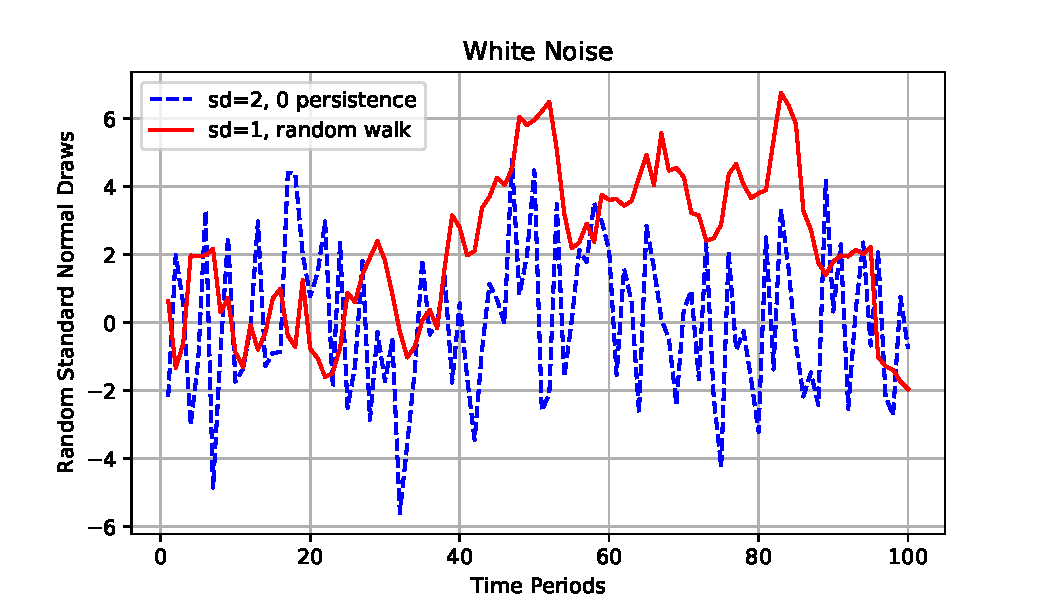
\includegraphics{Data-Structures-and-Cloud-Services-with-Python_files/figure-latex/unnamed-chunk-70-1} \end{center}

\hypertarget{text-plot}{%
\subsection{Text Plot}\label{text-plot}}

\begin{quote}
Go back to \href{http://fanwangecon.github.io/}{fan}'s \href{https://fanwangecon.github.io/pyfan/}{Python Code Examples} Repository (\href{https://fanwangecon.github.io/pyfan/bookdown}{bookdown site}).
\end{quote}

\hypertarget{plot-text}{%
\subsubsection{Plot Text}\label{plot-text}}

Plot Text as Image. \href{https://matplotlib.org/3.1.1/gallery/pyplots/text_layout.html\#sphx-glr-gallery-pyplots-text-layout-py}{Create text with different alignment and rotation.}

\begin{Shaded}
\begin{Highlighting}[]
\CommentTok{\# Import Packages}
\ImportTok{import}\NormalTok{ matplotlib.pyplot }\ImportTok{as}\NormalTok{ plt}
\ImportTok{import}\NormalTok{ textwrap}
\ImportTok{import}\NormalTok{ json}

\CommentTok{\# Dict of String to String}
\NormalTok{dc\_path }\OperatorTok{=}\NormalTok{ \{}\StringTok{\textquotesingle{}C:}\CharTok{\textbackslash{}\textbackslash{}}\StringTok{Users}\CharTok{\textbackslash{}\textbackslash{}}\StringTok{fan}\CharTok{\textbackslash{}\textbackslash{}}\StringTok{Documents}\CharTok{\textbackslash{}\textbackslash{}}\StringTok{Dropbox (UH{-}ECON)}\CharTok{\textbackslash{}\textbackslash{}}\StringTok{repos}\CharTok{\textbackslash{}\textbackslash{}}\StringTok{Tex4Econ}\CharTok{\textbackslash{}\textbackslash{}}\StringTok{\textquotesingle{}}
           \StringTok{\textquotesingle{}\_other}\CharTok{\textbackslash{}\textbackslash{}}\StringTok{equation}\CharTok{\textbackslash{}\textbackslash{}}\StringTok{cases.tex\textquotesingle{}}\NormalTok{:}
               \StringTok{\textquotesingle{}C:/Users/fan/Documents/cases.pdf\textquotesingle{}}\NormalTok{,}
           \StringTok{\textquotesingle{}C:}\CharTok{\textbackslash{}\textbackslash{}}\StringTok{Users}\CharTok{\textbackslash{}\textbackslash{}}\StringTok{fan}\CharTok{\textbackslash{}\textbackslash{}}\StringTok{Documents}\CharTok{\textbackslash{}\textbackslash{}}\StringTok{Dropbox (UH{-}ECON)}\CharTok{\textbackslash{}\textbackslash{}}\StringTok{repos}\CharTok{\textbackslash{}\textbackslash{}}\StringTok{Tex4Econ}\CharTok{\textbackslash{}\textbackslash{}}\StringTok{\textquotesingle{}}
           \StringTok{\textquotesingle{}\_other}\CharTok{\textbackslash{}\textbackslash{}}\StringTok{symbols}\CharTok{\textbackslash{}\textbackslash{}}\StringTok{fs\_symbols.tex\textquotesingle{}}\NormalTok{:}
               \StringTok{\textquotesingle{}C:/Users/fan/Documents/fs\_symbols.pdf\textquotesingle{}}\NormalTok{\}}
\NormalTok{st\_dc\_path }\OperatorTok{=}\NormalTok{ textwrap.fill(json.dumps(dc\_path), width }\OperatorTok{=} \DecValTok{70}\NormalTok{)}

\CommentTok{\# Start Plot}
\NormalTok{fig, ax }\OperatorTok{=}\NormalTok{ plt.subplots()}

\CommentTok{\# Text Plot}
\NormalTok{ax.text(}\FloatTok{0.5}\NormalTok{, }\FloatTok{0.5}\NormalTok{, st\_dc\_path,}
\NormalTok{        horizontalalignment}\OperatorTok{=}\StringTok{\textquotesingle{}center\textquotesingle{}}\NormalTok{,}
\NormalTok{        verticalalignment}\OperatorTok{=}\StringTok{\textquotesingle{}center\textquotesingle{}}\NormalTok{,}
\NormalTok{        fontsize}\OperatorTok{=}\DecValTok{14}\NormalTok{, color}\OperatorTok{=}\StringTok{\textquotesingle{}black\textquotesingle{}}\NormalTok{,}
\NormalTok{        transform}\OperatorTok{=}\NormalTok{ax.transAxes)}

\CommentTok{\# Labeling}
\end{Highlighting}
\end{Shaded}

\begin{verbatim}
## Text(0.5, 0.5, '{"C:\\\\Users\\\\fan\\\\Documents\\\\Dropbox (UH-\nECON)\\\\repos\\\\Tex4Econ\\\\_other\\\\equation\\\\cases.tex":\n"C:/Users/fan/Documents/cases.pdf",\n"C:\\\\Users\\\\fan\\\\Documents\\\\Dropbox (UH-\nECON)\\\\repos\\\\Tex4Econ\\\\_other\\\\symbols\\\\fs_symbols.tex":\n"C:/Users/fan/Documents/fs_symbols.pdf"}')
\end{verbatim}

\begin{Shaded}
\begin{Highlighting}[]
\NormalTok{ax.set\_axis\_off()}
\NormalTok{plt.show()}
\end{Highlighting}
\end{Shaded}

\begin{center}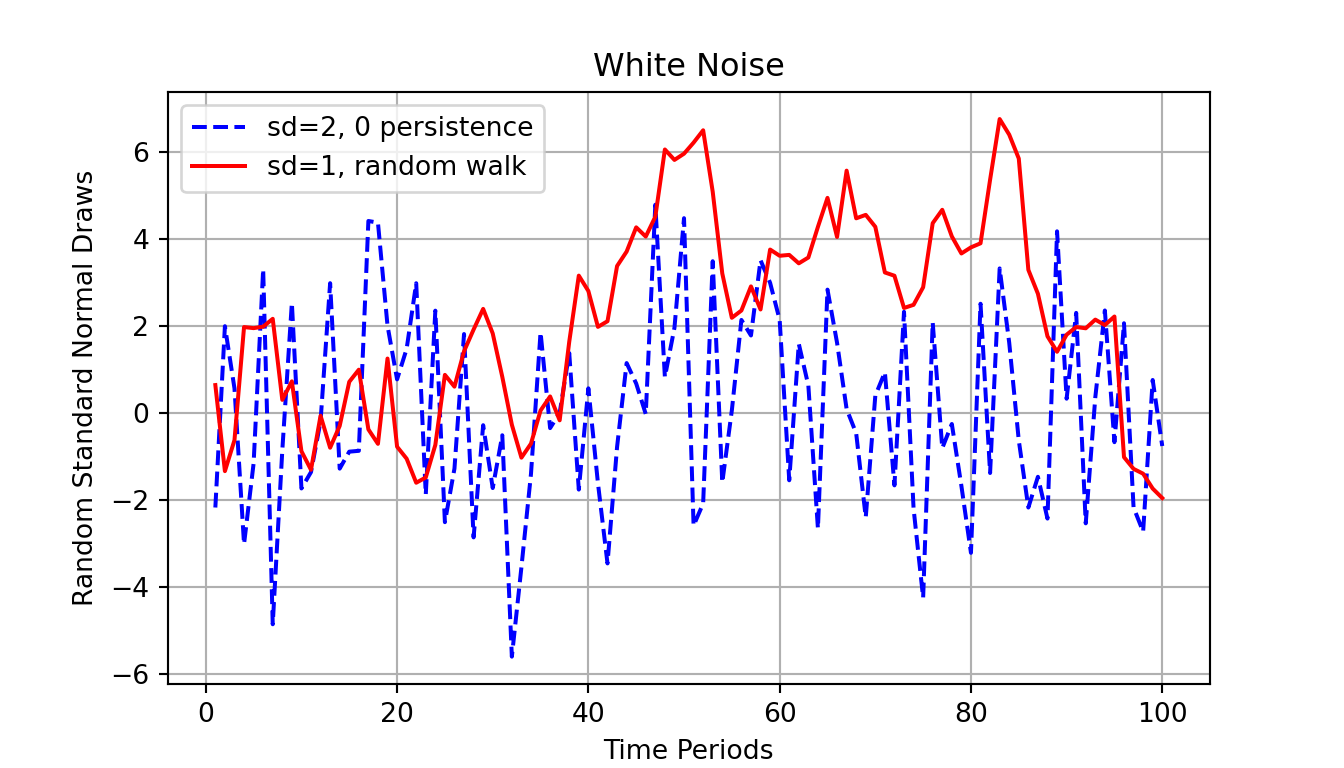
\includegraphics{Data-Structures-and-Cloud-Services-with-Python_files/figure-latex/unnamed-chunk-72-1} \end{center}

\hypertarget{amazon-web-services}{%
\chapter{Amazon Web Services}\label{amazon-web-services}}

\hypertarget{aws-setup}{%
\section{AWS Setup}\label{aws-setup}}

\hypertarget{aws-setup-1}{%
\subsection{AWS Setup}\label{aws-setup-1}}

\begin{quote}
Go back to \href{http://fanwangecon.github.io/}{fan}'s \href{https://fanwangecon.github.io/pyfan/}{Python Code Examples} Repository (\href{https://fanwangecon.github.io/pyfan/bookdown}{bookdown site}).
\end{quote}

\hypertarget{installation-on-local-machine}{%
\subsubsection{Installation on Local Machine}\label{installation-on-local-machine}}

First install \href{https://fanwangecon.github.io/Tex4Econ/nontex/install/windows/fn_installations.html}{anaconda, git, and associated programs}.

\begin{enumerate}
\def\labelenumi{\arabic{enumi}.}
\tightlist
\item
  Putty
\item
  access to .pem key
\item
  conda aws environment below
\end{enumerate}

\hypertarget{conda-aws-environment}{%
\subsubsection{Conda AWS Environment}\label{conda-aws-environment}}

Can Start and Stop instances from Conda Prompt after this.

\begin{verbatim}
conda deactivate
conda list env
conda env remove -n wk_aws
conda create -n wk_aws -y
conda activate wk_aws

# Install External Tools
conda install -c anaconda pip -y

# Command line interface
conda install -c conda-forge awscli -y
# Programmatically send JSON instructions with boto3
conda install -c anaconda boto3 -y
\end{verbatim}

\hypertarget{aws-account-set-up}{%
\subsubsection{AWS Account set-up}\label{aws-account-set-up}}

\begin{enumerate}
\def\labelenumi{\arabic{enumi}.}
\tightlist
\item
  Sign-up for AWS web services account (can be the same as your Amazon shopping account)
\item
  Register for \href{https://aws.amazon.com/education/awseducate/}{AWS Educate} to get student or faculty voucher.
\end{enumerate}

\begin{itemize}
\tightlist
\item
  The University of Houston is a part of AWS Educate, choose educator or student, should hear back within 24 hours with coupon code.
\item
  UH students can get \$100, faculty can get \$200.
\end{itemize}

\hypertarget{start-a-aws-instance-and-link-local-to-remote}{%
\subsubsection{Start a AWS Instance and Link Local to Remote}\label{start-a-aws-instance-and-link-local-to-remote}}

Amazon has a lot of tutorials. Here is an outline.

\begin{enumerate}
\def\labelenumi{\arabic{enumi}.}
\tightlist
\item
  Generate keypair on AWS, \href{https://docs.aws.amazon.com/AWSEC2/latest/UserGuide/ec2-key-pairs.html\#having-ec2-create-your-key-pair}{aws guide}

  \begin{itemize}
  \tightlist
  \item
    this gives you a .pem file which you download and Amazon also remembers
  \item
    local computers with the right .pem file can talk to your AWS instances
  \item
    You might need to invoke the chmod command below to set permission:
  \end{itemize}

\begin{Shaded}
\begin{Highlighting}[]
\FunctionTok{chmod}\NormalTok{ 400 }\StringTok{"C:/Users/fan/Documents/Dropbox (UH{-}ECON)/Programming/AWS/fan\_wang{-}key{-}pair{-}us\_east\_nv.pem"}
\end{Highlighting}
\end{Shaded}
\item
  \emph{Launching Instance}: Go to your console, choose EC2, choose launch instance, select Amazon Linux Instance (review and launch)
\item
  \emph{Instance security}: select VPC security group: I have for example: fan\_wang\_SG\_us\_east\_nv\_VPC (edit security group and submit)

  \begin{itemize}
  \tightlist
  \item
    Security group can allow any IP address to access your instance or just specific ones.
  \item
    AWS has a tool here that just allows your current IP to access the EC2 instance
  \end{itemize}
\item
  \emph{Instance access key}: Select right keypair (your .pem key), fan\_wang-key-pair-us\_east\_nv (prompted after submitting)
\item
  For SSH in, you can use Putty. \href{https://docs.aws.amazon.com/AWSEC2/latest/UserGuide/putty.html}{aws guide}

  \begin{itemize}
  \tightlist
  \item
    tell Putty your AWS instance DNS address and where your pem key is
  \item
    Can use a Putty client to enter an EC2 instance
  \end{itemize}
\item
  For SSH, can also do the process below:

  \begin{itemize}
  \tightlist
  \item
    \href{https://stackoverflow.com/questions/18683092/how-to-run-ssh-add-on-windows}{open git bash} (install putty before)
  \end{itemize}

\begin{Shaded}
\begin{Highlighting}[]
\FunctionTok{ssh{-}agent}\NormalTok{ {-}s}
\BuiltInTok{eval} \VariableTok{$(}\FunctionTok{ssh{-}agent}\NormalTok{ {-}s}\VariableTok{)}
\end{Highlighting}
\end{Shaded}

  \begin{itemize}
  \tightlist
  \item
    Tell SSH where pem key is:
  \end{itemize}

\begin{Shaded}
\begin{Highlighting}[]
\FunctionTok{ssh{-}add} \StringTok{"C:/Users/fan/Documents/Dropbox (UH{-}ECON)/Programming/AWS/fan\_wang{-}key{-}pair{-}us\_east\_nv.pem"}
\end{Highlighting}
\end{Shaded}

  \begin{itemize}
  \tightlist
  \item
    You will find a public DNS address for your aws instance on the AWS user interface page
  \end{itemize}

\begin{Shaded}
\begin{Highlighting}[]
\CommentTok{\# ssh git bash command line}
\CommentTok{\# for ubuntu machine}
\FunctionTok{ssh}\NormalTok{ ubuntu@ec2{-}54{-}197{-}6{-}153.compute{-}1.amazonaws.com}
\CommentTok{\# for aws linux}
\FunctionTok{ssh}\NormalTok{ ec2{-}user@ec2{-}52{-}23{-}218{-}117.compute{-}1.amazonaws.com}
\CommentTok{\# quit aws instance}
\CommentTok{\# ctrl + D}
\end{Highlighting}
\end{Shaded}

  \begin{itemize}
  \tightlist
  \item
    if get: Permission denied (publickey), see:

    \begin{enumerate}
    \def\labelenumii{\arabic{enumii}.}
    \tightlist
    \item
      Trying to connect with the wrong key. Are you sure this instance is using this keypair?
    \item
      Trying to connect with the wrong username. ubuntu is the username for the ubuntu based AWS distribution, but on some others it's ec2-user (or admin on some Debians, according to Bogdan Kulbida's answer)(can also be root, fedora, see below)
    \item
      Trying to connect the wrong host. Is that the right host you are trying to log in to?
    \end{enumerate}
  \item
    You can log in generally like this, note the instance gets new public DNS IP address every time you restart it:
  \end{itemize}

\begin{Shaded}
\begin{Highlighting}[]
\VariableTok{LOCALPEM=}\StringTok{"C:/Users/fan/Documents/Dropbox (UH{-}ECON)/Programming/AWS/fan\_wang{-}key{-}pair{-}us\_east\_nv.pem"}
\VariableTok{IPADD=}\NormalTok{34.207.250.160}
\VariableTok{REMOTEIP=}\NormalTok{ec2{-}user}\ExtensionTok{@}\VariableTok{$IPADD}
\FunctionTok{ssh{-}keygen}\NormalTok{ {-}R }\VariableTok{$IPADD}
\FunctionTok{ssh}\NormalTok{ {-}i }\StringTok{"}\VariableTok{$LOCALPEM}\StringTok{"} \VariableTok{$REMOTEIP}
\end{Highlighting}
\end{Shaded}
\end{enumerate}

\hypertarget{use-awscli-to-start-and-stop-an-instance}{%
\subsubsection{Use AWSCLI to Start and Stop an Instance}\label{use-awscli-to-start-and-stop-an-instance}}

\begin{enumerate}
\def\labelenumi{\arabic{enumi}.}
\tightlist
\item
  Install AWS CLI
\item
  Create individual IAM users
\item
  Follow instructions to \href{https://docs.aws.amazon.com/cli/latest/userguide/cli-chap-getting-started.html}{Configure your awscli}, and profit access key id and secrete access key when prompted.

  \begin{itemize}
  \tightlist
  \item
    do not copy and paste the Key ID and Access Key. They are example, type these in as answers given config prompt:
  \end{itemize}

\begin{Shaded}
\begin{Highlighting}[]
\CommentTok{\# aws configure}
\ExtensionTok{AWS}\NormalTok{ Access Key ID [None]: XXXXIOSFODNN7EXAMPLE}
\ExtensionTok{AWS}\NormalTok{ Secret Access Key [None]: wXalrXXtnXXXX/X7XXXXX/bXxXfiCXXXXXXXXXXX}
\ExtensionTok{Default}\NormalTok{ region name [None]: us{-}west{-}1}
\ExtensionTok{Default}\NormalTok{ output format [None]: json}
\end{Highlighting}
\end{Shaded}

  \begin{itemize}
  \tightlist
  \item
    this creates under a folder like this: C:/Users/fan/.aws, inside the folder these info will be stored in a configuration file.
  \end{itemize}

\begin{Shaded}
\begin{Highlighting}[]
\CommentTok{\# the credentials file}
\NormalTok{[}\ExtensionTok{default}\NormalTok{]}
\ExtensionTok{aws\_access\_key\_id}\NormalTok{ = XXXXIOSFODNN7EXAMPLE}
\ExtensionTok{aws\_secret\_access\_key}\NormalTok{ = wXalrXXtnXXXXX7XXXXXbXxXfiCXXXXXXXXXXX}
\end{Highlighting}
\end{Shaded}

  \begin{itemize}
  \tightlist
  \item
    then when you use aws cli, you will automatically be authenticated
  \end{itemize}
\item
  Start an instance in console first (or directly in command line). Stop it. do not terminate. Now this instance will have a fixed instance ID. Its DNS IP address will change every time you restart it, but its instance ID is fixed. Instance ID is found easily in the EC2 Console.

  \begin{itemize}
  \tightlist
  \item
    \href{https://docs.aws.amazon.com/cli/latest/userguide/cli-ec2-launch.html}{Launch an instance}
  \end{itemize}

\begin{Shaded}
\begin{Highlighting}[]
\ExtensionTok{aws}\NormalTok{ ec2 run{-}instances {-}{-}image{-}id ami{-}xxxxxxxx {-}{-}count 1 {-}{-}instance{-}type t2.micro {-}{-}key{-}name MyKeyPair {-}{-}security{-}group{-}ids sg{-}xxxxxxxx {-}{-}subnet{-}id subnet{-}xxxxxxxx}
\end{Highlighting}
\end{Shaded}

  \begin{itemize}
  \tightlist
  \item
    \href{https://docs.aws.amazon.com/cli/latest/reference/ec2/start-instances.html}{Start} an instance
  \end{itemize}

\begin{Shaded}
\begin{Highlighting}[]
\ExtensionTok{aws}\NormalTok{ ec2 start{-}instances {-}{-}instance{-}ids i{-}XXXXXXXX}
\ExtensionTok{aws}\NormalTok{ ec2 start{-}instances {-}{-}instance{-}ids i{-}040c856530b2619bc}
\end{Highlighting}
\end{Shaded}

  \begin{itemize}
  \tightlist
  \item
    \href{https://docs.aws.amazon.com/cli/latest/reference/ec2/stop-instances.html}{Stop} an instance
  \end{itemize}

\begin{Shaded}
\begin{Highlighting}[]
\ExtensionTok{aws}\NormalTok{ ec2 stop{-}instances {-}{-}instance{-}ids i{-}XXXXXXXX}
\ExtensionTok{aws}\NormalTok{ ec2 stop{-}instances {-}{-}instance{-}ids i{-}040c856530b2619bc}
\end{Highlighting}
\end{Shaded}
\end{enumerate}

\hypertarget{set-up-ssm-on-ec2-instance}{%
\subsubsection{Set-up SSM on EC2 Instance}\label{set-up-ssm-on-ec2-instance}}

To execute commandlines etc remote on EC2, need to set up SSM: AWS Systems Manager Agent (\href{https://docs.aws.amazon.com/systems-manager/latest/userguide/ssm-agent.html}{SSM Agent})

SSM-agent is already installed in Amazon Linux.

\href{https://stackoverflow.com/questions/47034797/invalidinstanceid-an-error-occurred-invalidinstanceid-when-calling-the-sendco}{Error Message regarding InvalidInstanceId}. The following scenarios can result in this error message:

\begin{itemize}
\tightlist
\item
  Instance id is invalid (in the comments you have verified it isn't)
\item
  Instance is in a different region (in the comments you have verified it isn't)
\item
  Instance is not currently in the Running state
\item
  Instance does not have the AWS SSM agent installed and running.
\end{itemize}

``You have to create and attach the policy AmazonSSMFullAccess to the machine (thats maybe more broad than you need) but that was why it wasn't working for me\ldots{} You do that by clicking on (when selected on the ec2 instance) Action \textgreater{} Instance Settings \textgreater{} Attach/Replace IAM Role then create a role for ec2 that has that permission then attach, should take like 5-10 mins to pop up in SYSTEMS MANAGER SHARED RESOURCES - Managed Instances as mark mentions. -- Glen Thompson Sep 20 '18 at 16:31''

\begin{Shaded}
\begin{Highlighting}[]
\CommentTok{\# Start SSM Agent with}
\FunctionTok{sudo}\NormalTok{ systemctl start amazon{-}ssm{-}agent}
\end{Highlighting}
\end{Shaded}

\hypertarget{aws-boto3}{%
\subsection{AWS Boto3}\label{aws-boto3}}

\begin{quote}
Go back to \href{http://fanwangecon.github.io/}{fan}'s \href{https://fanwangecon.github.io/pyfan/}{Python Code Examples} Repository (\href{https://fanwangecon.github.io/pyfan/bookdown}{bookdown site}).
\end{quote}

\hypertarget{basics}{%
\subsubsection{Basics}\label{basics}}

Create local .aws folder under user for example that has credential information, this will be useful for AWS command line operations.

\begin{Shaded}
\begin{Highlighting}[]
\CommentTok{\# IN C:\textbackslash{}Users\textbackslash{}fan\textbackslash{}.aws}
\CommentTok{\# config file}
\NormalTok{[}\ExtensionTok{default}\NormalTok{]}
\ExtensionTok{region}\NormalTok{ = us{-}east{-}1}
\ExtensionTok{output}\NormalTok{ = json}
\CommentTok{\# credentials file}
\NormalTok{[}\ExtensionTok{default}\NormalTok{]}
\ExtensionTok{aws\_access\_key\_id}\NormalTok{ = XKIXXXGSXXXBZXX43XXX}
\ExtensionTok{aws\_secret\_access\_key}\NormalTok{ = xxTgp9r0f4XXXXXXX1XXlG1vTy07wydxXXXXXX11}
\end{Highlighting}
\end{Shaded}

Additionally, or alternatively, for boto3 operations, store in for example a yml file, so that appropriate value could be obtained.

\begin{Shaded}
\begin{Highlighting}[]
\KeywordTok{{-}}\AttributeTok{ }\FunctionTok{main\_aws\_id}\KeywordTok{:}\AttributeTok{ 710673677961,}
\AttributeTok{  }\FunctionTok{aws\_access\_key\_id}\KeywordTok{:}\AttributeTok{ XKIXXXGSXXXBZXX43XXX}
\AttributeTok{  }\FunctionTok{aws\_secret\_access\_key}\KeywordTok{:}\AttributeTok{ xxTgp9r0f4XXXXXXX1XXlG1vTy07wydxXXXXXX11}
\AttributeTok{  }\FunctionTok{region}\KeywordTok{:}\AttributeTok{ us{-}east{-}1}
\AttributeTok{  }\FunctionTok{main\_ec2\_instance\_id}\KeywordTok{:}\AttributeTok{ i{-}YYYxYYYYYYx2619xx}
\AttributeTok{  }\FunctionTok{main\_ec2\_linux\_ami}\KeywordTok{:}\AttributeTok{ ami{-}0xYYYYYxx95x71x9}
\AttributeTok{  }\FunctionTok{main\_ec2\_public\_subnet}\KeywordTok{:}\AttributeTok{ subnet{-}d9xxxxYY}
\AttributeTok{  }\FunctionTok{fargate\_vpc\_name}\KeywordTok{:}\AttributeTok{ FanCluster}
\AttributeTok{  }\FunctionTok{fargate\_vpc\_id}\KeywordTok{:}\AttributeTok{ vpc{-}xxx5xYYY}
\AttributeTok{  }\FunctionTok{fargate\_public\_subnet}\KeywordTok{:}\AttributeTok{ subnet{-}e3dYYYxx}
\AttributeTok{  }\FunctionTok{fargate\_security\_group}\KeywordTok{:}\AttributeTok{ sg{-}17xxxxYx}
\AttributeTok{  }\FunctionTok{fargate\_task\_executionRoleArn}\KeywordTok{:}\AttributeTok{ ecsTaskExecutionRole}
\AttributeTok{  }\FunctionTok{batch\_task\_executionRoleArn}\KeywordTok{:}\AttributeTok{ ecsExecutionRole}
\AttributeTok{  }\FunctionTok{fargate\_route\_table}\KeywordTok{:}\AttributeTok{ rtb{-}5xxxYx25}
\AttributeTok{  }\FunctionTok{date\_start}\KeywordTok{:}\AttributeTok{ }\DecValTok{20180701}
\end{Highlighting}
\end{Shaded}

\hypertarget{start-client-service}{%
\subsubsection{Start Client Service}\label{start-client-service}}

For the various AWS services, could use Boto3 to access and use programmatically. To use any particular service, first start the client for that service: \href{https://boto3.amazonaws.com/v1/documentation/api/latest/reference/core/session.html\#boto3.session.Session.client}{boto3 client}.

We load AWS access key and secret acess key etc in from a \href{https://fanwangecon.github.io/pyfan/vig/support/inout/htmlpdfr/fp_yaml.html}{yaml file} to start boto3 client. We then start the client for \href{https://aws.amazon.com/batch/}{AWS Batch}. And then describe a \href{https://boto3.amazonaws.com/v1/documentation/api/latest/reference/services/batch.html\#Batch.Client.describe_compute_environments}{compute environment}.

\begin{Shaded}
\begin{Highlighting}[]
\ImportTok{import}\NormalTok{ boto3}
\ImportTok{import}\NormalTok{ yaml}
\ImportTok{import}\NormalTok{ pprint}

\CommentTok{\# Load YAML file}
\NormalTok{son\_aws\_yml }\OperatorTok{=} \StringTok{"C:/Users/fan/fanwangecon.github.io/\_data/aws.yml"}
\NormalTok{fl\_yaml }\OperatorTok{=} \BuiltInTok{open}\NormalTok{(son\_aws\_yml)}
\NormalTok{ls\_dict\_yml }\OperatorTok{=}\NormalTok{ yaml.load(fl\_yaml, Loader}\OperatorTok{=}\NormalTok{yaml.BaseLoader)}
\CommentTok{\# Get the first element of the yml list of dicts}
\NormalTok{aws\_yml\_dict\_yml }\OperatorTok{=}\NormalTok{ ls\_dict\_yml[}\DecValTok{0}\NormalTok{]}

\CommentTok{\# Use AWS Personal Access Keys etc to start boto3 client}
\NormalTok{aws\_batch }\OperatorTok{=}\NormalTok{ boto3.client(}\StringTok{\textquotesingle{}batch\textquotesingle{}}\NormalTok{,}
\NormalTok{  aws\_access\_key\_id}\OperatorTok{=}\NormalTok{aws\_yml\_dict\_yml[}\StringTok{\textquotesingle{}aws\_access\_key\_id\textquotesingle{}}\NormalTok{],}
\NormalTok{  aws\_secret\_access\_key}\OperatorTok{=}\NormalTok{aws\_yml\_dict\_yml[}\StringTok{\textquotesingle{}aws\_secret\_access\_key\textquotesingle{}}\NormalTok{],}
\NormalTok{  region\_name}\OperatorTok{=}\NormalTok{aws\_yml\_dict\_yml[}\StringTok{\textquotesingle{}region\textquotesingle{}}\NormalTok{])}

\CommentTok{\# Show a compute environment Delete some Personal Information}
\NormalTok{ob\_response }\OperatorTok{=}\NormalTok{ aws\_batch.describe\_compute\_environments(computeEnvironments}\OperatorTok{=}\NormalTok{[}\StringTok{"SpotEnv2560"}\NormalTok{])}
\NormalTok{ob\_response[}\StringTok{\textquotesingle{}ResponseMetadata\textquotesingle{}}\NormalTok{] }\OperatorTok{=} \StringTok{\textquotesingle{}\textquotesingle{}}
\NormalTok{ob\_response[}\StringTok{\textquotesingle{}computeEnvironments\textquotesingle{}}\NormalTok{][}\DecValTok{0}\NormalTok{][}\StringTok{\textquotesingle{}ecsClusterArn\textquotesingle{}}\NormalTok{] }\OperatorTok{=} \StringTok{\textquotesingle{}\textquotesingle{}}
\NormalTok{ob\_response[}\StringTok{\textquotesingle{}computeEnvironments\textquotesingle{}}\NormalTok{][}\DecValTok{0}\NormalTok{][}\StringTok{\textquotesingle{}serviceRole\textquotesingle{}}\NormalTok{] }\OperatorTok{=} \StringTok{\textquotesingle{}\textquotesingle{}}
\NormalTok{ob\_response[}\StringTok{\textquotesingle{}computeEnvironments\textquotesingle{}}\NormalTok{][}\DecValTok{0}\NormalTok{][}\StringTok{\textquotesingle{}computeResources\textquotesingle{}}\NormalTok{][}\StringTok{\textquotesingle{}instanceRole\textquotesingle{}}\NormalTok{] }\OperatorTok{=} \StringTok{\textquotesingle{}\textquotesingle{}}
\NormalTok{pprint.pprint(ob\_response, width}\OperatorTok{=}\DecValTok{1}\NormalTok{)}
\end{Highlighting}
\end{Shaded}

\begin{verbatim}
## {'ResponseMetadata': '',
##  'computeEnvironments': [{'computeEnvironmentArn': 'arn:aws:batch:us-east-1:710673677961:compute-environment/SpotEnv2560',
##                           'computeEnvironmentName': 'SpotEnv2560',
##                           'computeResources': {'desiredvCpus': 0,
##                                                'ec2KeyPair': 'fan_wang-key-pair-us_east_nv',
##                                                'instanceRole': '',
##                                                'instanceTypes': ['optimal'],
##                                                'maxvCpus': 2560,
##                                                'minvCpus': 0,
##                                                'securityGroupIds': ['sg-e6642399'],
##                                                'spotIamFleetRole': 'arn:aws:iam::710673677961:role/AmazonEC2SpotFleetRole',
##                                                'subnets': ['subnet-d9abbe82'],
##                                                'tags': {},
##                                                'type': 'SPOT'},
##                           'ecsClusterArn': '',
##                           'serviceRole': '',
##                           'state': 'ENABLED',
##                           'status': 'VALID',
##                           'statusReason': 'ComputeEnvironment '
##                                           'Healthy',
##                           'tags': {},
##                           'type': 'MANAGED'}]}
\end{verbatim}

\hypertarget{s3}{%
\section{S3}\label{s3}}

\hypertarget{s3-usages}{%
\subsection{S3 Usages}\label{s3-usages}}

\begin{quote}
Go back to \href{http://fanwangecon.github.io/}{fan}'s \href{https://fanwangecon.github.io/pyfan/}{Python Code Examples} Repository (\href{https://fanwangecon.github.io/pyfan/bookdown}{bookdown site}).
\end{quote}

\hypertarget{upload-local-file-to-s3}{%
\subsubsection{Upload Local File to S3}\label{upload-local-file-to-s3}}

A program runs either locally or on a remote EC2 machine inside a docker container. Upon exit, data does not persist in the docker container and needs to be exported to be saved. The idea is to export program images, csv files, json files, etc to S3 when these are generated, if the program detects that it is been executed on an EC2 machine (in a container).

First, inside the program, detect platform status. For Docker Container on EC2, AWS Linux 2 has platform.release of something like \emph{4.14.193-194.317.amzn2.x86\_64}.

\begin{Shaded}
\begin{Highlighting}[]
\ImportTok{import}\NormalTok{ platform }\ImportTok{as}\NormalTok{ platform}
\BuiltInTok{print}\NormalTok{(platform.release())}
\CommentTok{\# This assums using an EC2 instance where amzn is in platform name}
\end{Highlighting}
\end{Shaded}

\begin{verbatim}
## 10
\end{verbatim}

\begin{Shaded}
\begin{Highlighting}[]
\ControlFlowTok{if} \StringTok{\textquotesingle{}amzn\textquotesingle{}} \KeywordTok{in}\NormalTok{ platform.release():}
\NormalTok{    s3\_status }\OperatorTok{=} \VariableTok{True}
\ControlFlowTok{else}\NormalTok{:}
\NormalTok{    s3\_status }\OperatorTok{=} \VariableTok{False}
\BuiltInTok{print}\NormalTok{(s3\_status)}
\end{Highlighting}
\end{Shaded}

\begin{verbatim}
## False
\end{verbatim}

Second, on s3, create a bucket, \emph{fans3testbucket} for example (no underscore in name allowed). Before doing this, set up AWS Access Key ID and AWS Secrete Acccess KEy in \emph{/Users/fan/.aws} folder so that boto3 can access s3 from computer. Upon successful completion of the push, the file can be accessed at \url{https://fans3testbucket.s3.amazonaws.com/_data/iris_s3.dta}.

\begin{Shaded}
\begin{Highlighting}[]
\ImportTok{import}\NormalTok{ boto3}
\NormalTok{s3 }\OperatorTok{=}\NormalTok{ boto3.client(}\StringTok{\textquotesingle{}s3\textquotesingle{}}\NormalTok{)}
\NormalTok{spn\_local\_path\_file\_name }\OperatorTok{=} \StringTok{"C:/Users/fan/pyfan/vig/aws/setup/\_data/iris\_s3.dta"}
\NormalTok{str\_bucket\_name }\OperatorTok{=} \StringTok{"fans3testbucket"}
\NormalTok{spn\_remote\_path\_file\_name }\OperatorTok{=} \StringTok{"\_data/iris\_s3.dta"}
\NormalTok{s3.upload\_file(spn\_local\_path\_file\_name, str\_bucket\_name, spn\_remote\_path\_file\_name)}
\end{Highlighting}
\end{Shaded}

\hypertarget{batch}{%
\section{Batch}\label{batch}}

\hypertarget{aws-batch-run}{%
\subsection{AWS Batch Run}\label{aws-batch-run}}

\begin{quote}
Go back to \href{http://fanwangecon.github.io/}{fan}'s \href{https://fanwangecon.github.io/pyfan/}{Python Code Examples} Repository (\href{https://fanwangecon.github.io/pyfan/bookdown}{bookdown site}).
\end{quote}

\hypertarget{preparing-a-docker-image-and-a-python-function-for-batch-array-job}{%
\subsubsection{Preparing a Docker Image and a Python Function for Batch Array Job}\label{preparing-a-docker-image-and-a-python-function-for-batch-array-job}}

We want to set-up a function that can be used jointly with \href{https://docs.aws.amazon.com/batch/latest/userguide/array_jobs.html}{AWS Batch Array}. With Batch Array, can run many simulations concurrently. All simulations might only differ in random seed for drawing shocks. This requires setting up the proper dockerfile as well as modifying the python function that we want to invoke slightly.

First, create and push a docker image, see this \href{https://fanwangecon.github.io/pyfan/vig/docker/setup/htmlpdfr/fs_docker_ecr.html\#141_Example_Docker_File_for_AWS}{dockerfile}. Following the AWS ECR instructions, this registers a docker image in AWS ECR with a URI: \emph{XXXX7367XXXX.dkr.ecr.us-east-1.amazonaws.com/fanconda}

The \href{https://fanwangecon.github.io/pyfan/vig/docker/setup/htmlpdfr/fs_docker_ecr.html\#141_Example_Docker_File_for_AWS}{dockerfile} has for CMD: \emph{CMD {[}``python'', ``/pyfan/pyfan/graph/exa/scatterline3.py''{]}}. This runs the function \href{https://github.com/FanWangEcon/pyfan/blob/master/pyfan/graph/exa/scatterline3.py}{scatterline3}.

Second, the \href{https://github.com/FanWangEcon/pyfan/blob/master/pyfan/graph/exa/scatterline3.py}{scatterline3} function checks if \href{https://github.com/FanWangEcon/pyfan/blob/master/pyfan/graph/exa/scatterline3.py\#L167}{\emph{AWS\_BATCH\_JOB\_ARRAY\_INDEX} is in the \emph{os.environ}}. \emph{AWS\_BATCH\_JOB\_ARRAY\_INDEX}, if exists, is used as a random seed to generate data for the graph. When the function is run in a docker container via batch, the function saves the graph output to a bucket in AWS s3. The pushing the s3 is achieved by \href{https://github.com/FanWangEcon/pyfan/blob/master/pyfan/aws/general/path.py}{pyfan.aws.general.path.py}.

In the batch job, when \emph{arrayProperties = \{`size': 10\}}, this will generate \emph{AWS\_BATCH\_JOB\_ARRAY\_INDEX} from 1 through 10 in 10 sub-tasks of a single batch task. These \emph{AWS\_BATCH\_JOB\_ARRAY\_INDEX} could be used as different random seeds, and could be used as folder suffixes.

Here, the \href{https://github.com/FanWangEcon/pyfan/blob/master/pyfan/graph/exa/scatterline3.py}{scatterline3} function generates a graph, that will be stored for testing purpose in \href{https://s3.console.aws.amazon.com/s3/buckets/fans3testbucket/pyfan_gph_scatter_line_rand/?region=us-east-1\&tab=overview}{pyfan\_gph\_scatter\_line\_rand folder of fans3testbucket bucket}, the images saved has \emph{seed\_0.png}, \emph{seed\_1.png}, \ldots, \emph{seed\_10.png} as names when \emph{arrayProperties = \{`size': 10\}}.

\hypertarget{register-a-batch-job-definition}{%
\subsubsection{Register A Batch Job Definition}\label{register-a-batch-job-definition}}

Given the docker image we created: \emph{XXXX7367XXXX.dkr.ecr.us-east-1.amazonaws.com/fanconda}, we can use this to register a batch job.

\begin{enumerate}
\def\labelenumi{\arabic{enumi}.}
\tightlist
\item
  computing requirements: memory and cpu: \emph{vCpus = 1} and \emph{Memory=7168} for example
\item
  which container to pull from (ECR): List the image name: \emph{XXXX7367XXXX.dkr.ecr.us-east-1.amazonaws.com/fanconda} for example
\item
  job role ARN: \emph{arn:aws:iam::XXXX7367XXXX:role/ecsExecutionRole} to allow for proper in and out from and to the container.
\end{enumerate}

These can be registered programmatically by using boto3: \href{https://boto3.amazonaws.com/v1/documentation/api/latest/reference/services/batch.html}{Boto3 Batch Documentation}

In the example below, will register a new job definition, this will add \emph{pyfan-scatterline3-test-rmd} to \href{https://console.aws.amazon.com/batch/v2/home?region=us-east-1\#job-definition}{job definition} as an additional job definition.

Everytime, when the code below is re-run, a new batch revision number is generated. AWS allows per batch job to have potential hundreds of thousands of revisions.

\begin{Shaded}
\begin{Highlighting}[]
\ImportTok{import}\NormalTok{ boto3}
\ImportTok{import}\NormalTok{ yaml}
\ImportTok{import}\NormalTok{ pprint}

\CommentTok{\# Load YAML file with security info}
\NormalTok{srn\_aws\_yml }\OperatorTok{=} \StringTok{"C:/Users/fan/fanwangecon.github.io/\_data/aws.yml"}
\NormalTok{fl\_yaml }\OperatorTok{=} \BuiltInTok{open}\NormalTok{(srn\_aws\_yml)}
\NormalTok{ls\_dict\_yml }\OperatorTok{=}\NormalTok{ yaml.load(fl\_yaml, Loader}\OperatorTok{=}\NormalTok{yaml.BaseLoader)}
\NormalTok{aws\_yml\_dict\_yml }\OperatorTok{=}\NormalTok{ ls\_dict\_yml[}\DecValTok{0}\NormalTok{]}

\CommentTok{\# Dictionary storing job definition related information}
\NormalTok{job\_dict }\OperatorTok{=}\NormalTok{ \{}\StringTok{"jobDefinitionName"}\NormalTok{: }\StringTok{\textquotesingle{}pyfan{-}scatterline3{-}test{-}rmd\textquotesingle{}}\NormalTok{,}
            \StringTok{"type"}\NormalTok{: }\StringTok{"container"}\NormalTok{,}
            \StringTok{"containerProperties"}\NormalTok{: \{}
                \StringTok{"image"}\NormalTok{: aws\_yml\_dict\_yml[}\StringTok{\textquotesingle{}main\_aws\_id\textquotesingle{}}\NormalTok{] }\OperatorTok{+} \StringTok{".dkr.ecr."} \OperatorTok{+}
\NormalTok{                         aws\_yml\_dict\_yml[}\StringTok{\textquotesingle{}region\textquotesingle{}}\NormalTok{] }\OperatorTok{+} \StringTok{".amazonaws.com/fanconda"}\NormalTok{,}
                \StringTok{"vcpus"}\NormalTok{: }\BuiltInTok{int}\NormalTok{(}\DecValTok{1}\NormalTok{),}
                \StringTok{"memory"}\NormalTok{: }\BuiltInTok{int}\NormalTok{(}\DecValTok{1024}\NormalTok{),}
                \StringTok{"command"}\NormalTok{: [}\StringTok{"python"}\NormalTok{,}
                            \StringTok{"/pyfan/pyfan/graph/exa/scatterline3.py"}\NormalTok{,}
                            \StringTok{"{-}A"}\NormalTok{, }\StringTok{"fans3testbucket"}\NormalTok{,}
                            \StringTok{"{-}B"}\NormalTok{, }\StringTok{"111"}\NormalTok{],}
                \StringTok{"jobRoleArn"}\NormalTok{: }\StringTok{"arn:aws:iam::"} \OperatorTok{+}\NormalTok{ aws\_yml\_dict\_yml[}\StringTok{\textquotesingle{}main\_aws\_id\textquotesingle{}}\NormalTok{] }\OperatorTok{+}
                              \StringTok{":role/"} \OperatorTok{+}\NormalTok{ aws\_yml\_dict\_yml[}\StringTok{\textquotesingle{}batch\_task\_executionRoleArn\textquotesingle{}}\NormalTok{]}
\NormalTok{            \},}
            \StringTok{"retryStrategy"}\NormalTok{: \{}
                \StringTok{"attempts"}\NormalTok{: }\DecValTok{1}
\NormalTok{            \}\}}

\CommentTok{\# Use AWS Personal Access Keys etc to start boto3 client}
\NormalTok{aws\_batch }\OperatorTok{=}\NormalTok{ boto3.client(}\StringTok{\textquotesingle{}batch\textquotesingle{}}\NormalTok{,}
\NormalTok{  aws\_access\_key\_id}\OperatorTok{=}\NormalTok{aws\_yml\_dict\_yml[}\StringTok{\textquotesingle{}aws\_access\_key\_id\textquotesingle{}}\NormalTok{],}
\NormalTok{  aws\_secret\_access\_key}\OperatorTok{=}\NormalTok{aws\_yml\_dict\_yml[}\StringTok{\textquotesingle{}aws\_secret\_access\_key\textquotesingle{}}\NormalTok{],}
\NormalTok{  region\_name}\OperatorTok{=}\NormalTok{aws\_yml\_dict\_yml[}\StringTok{\textquotesingle{}region\textquotesingle{}}\NormalTok{])}

\CommentTok{\# Register a job definition}
\NormalTok{response }\OperatorTok{=}\NormalTok{ aws\_batch.register\_job\_definition(}
\NormalTok{        jobDefinitionName }\OperatorTok{=}\NormalTok{ job\_dict[}\StringTok{\textquotesingle{}jobDefinitionName\textquotesingle{}}\NormalTok{],}
        \BuiltInTok{type} \OperatorTok{=}\NormalTok{ job\_dict[}\StringTok{\textquotesingle{}type\textquotesingle{}}\NormalTok{],}
\NormalTok{        containerProperties }\OperatorTok{=}\NormalTok{ job\_dict[}\StringTok{\textquotesingle{}containerProperties\textquotesingle{}}\NormalTok{],}
\NormalTok{        retryStrategy }\OperatorTok{=}\NormalTok{ job\_dict[}\StringTok{\textquotesingle{}retryStrategy\textquotesingle{}}\NormalTok{])}

\CommentTok{\# Print response}
\NormalTok{pprint.pprint(response, width}\OperatorTok{=}\DecValTok{1}\NormalTok{)}
\end{Highlighting}
\end{Shaded}

\begin{verbatim}
## {'ResponseMetadata': {'HTTPHeaders': {'connection': 'keep-alive',
##                                       'content-length': '169',
##                                       'content-type': 'application/json',
##                                       'date': 'Sun, '
##                                               '29 '
##                                               'Nov '
##                                               '2020 '
##                                               '17:52:13 '
##                                               'GMT',
##                                       'x-amz-apigw-id': 'Wx_oKEGhoAMFSxQ=',
##                                       'x-amzn-requestid': '3125542c-4c35-4a6f-90e3-1999d92a8303',
##                                       'x-amzn-trace-id': 'Root=1-5fc3dfcd-10f402af14efabb06b02ec5d;Sampled=0'},
##                       'HTTPStatusCode': 200,
##                       'RequestId': '3125542c-4c35-4a6f-90e3-1999d92a8303',
##                       'RetryAttempts': 0},
##  'jobDefinitionArn': 'arn:aws:batch:us-east-1:710673677961:job-definition/pyfan-scatterline3-test-rmd:38',
##  'jobDefinitionName': 'pyfan-scatterline3-test-rmd',
##  'revision': 38}
\end{verbatim}

\hypertarget{submit-a-batch-array}{%
\subsubsection{Submit a Batch Array}\label{submit-a-batch-array}}

Given the batch job definition that has been created. Create also Job Queues and related compute environments. Then we can run Batch Array. Upon submitting the batch array, you can monitor AWS EC2 instances, should notice potentially many instances of EC2 starting up. AWS is starting EC2 instances to complete the batch array jobs.

create a \href{https://docs.aws.amazon.com/batch/latest/userguide/compute_environments.html}{batch compute environment} that uses \href{https://aws.amazon.com/ec2/pricing/}{spot price instances}, which will be much cheaper than on demand costs. Will need to set proper AMI roles, \emph{arn:aws:iam::XXXX7367XXXX:role/AmazonEC2SpotFleetRole} for \emph{Spot fleet role}, and also proper securities.

When the \emph{array\_size} parameter is equal to 100, that starts 100 child processes, with 1 through 100 for \emph{AWS\_BATCH\_JOB\_ARRAY\_INDEX}, which, could be used directly by the python function by taking in the parameter from the os environment as shown earlier. For demonstration purposes, will only set \emph{array\_size=3} in the example below.

Outputs from the \href{https://github.com/FanWangEcon/pyfan/blob/master/pyfan/graph/exa/scatterline3.py\#L138}{scatterline3} has a timestamp, so each time the code below is run, will generate several new images, with the same set of random seeds, but different date prefix. The output \href{https://s3.console.aws.amazon.com/s3/buckets/fans3testbucket/pyfan_gph_scatter_line_rand/?region=us-east-1\&tab=overview}{s3 folder is public}.

\begin{Shaded}
\begin{Highlighting}[]
\ImportTok{import}\NormalTok{ boto3}
\ImportTok{import}\NormalTok{ yaml}
\ImportTok{import}\NormalTok{ pprint}

\ImportTok{import}\NormalTok{ datetime }\ImportTok{as}\NormalTok{ datetime}

\CommentTok{\# Using the "jobDefinitionName": \textquotesingle{}pyfan{-}scatterline3{-}test{-}rmd\textquotesingle{} from registering}
\NormalTok{jobDefinitionName }\OperatorTok{=} \StringTok{\textquotesingle{}pyfan{-}scatterline3{-}test{-}rmd\textquotesingle{}}

\CommentTok{\# How many child batch processes to start}
\CommentTok{\# child process differ in: AWS\_BATCH\_JOB\_ARRAY\_INDEX}
\NormalTok{array\_size }\OperatorTok{=} \DecValTok{3}

\CommentTok{\# job name}
\NormalTok{timestr }\OperatorTok{=} \StringTok{"\{:\%Y\%m}\SpecialCharTok{\%d}\StringTok{\%H\%M\%S}\SpecialCharTok{\%f}\StringTok{\}"}\NormalTok{.}\BuiltInTok{format}\NormalTok{(datetime.datetime.now())}
\NormalTok{timesufx }\OperatorTok{=} \StringTok{\textquotesingle{}\_\textquotesingle{}} \OperatorTok{+}\NormalTok{ timestr}
\NormalTok{st\_jobName }\OperatorTok{=}\NormalTok{ jobDefinitionName }\OperatorTok{+}\NormalTok{ timesufx}

\CommentTok{\# job queue (needs to design own queue in batch)}
\NormalTok{st\_jobQueue }\OperatorTok{=} \StringTok{\textquotesingle{}Spot\textquotesingle{}}

\CommentTok{\# start batch service}
\CommentTok{\# Load YAML file with security info}
\NormalTok{srn\_aws\_yml }\OperatorTok{=} \StringTok{"C:/Users/fan/fanwangecon.github.io/\_data/aws.yml"}
\NormalTok{fl\_yaml }\OperatorTok{=} \BuiltInTok{open}\NormalTok{(srn\_aws\_yml)}
\NormalTok{ls\_dict\_yml }\OperatorTok{=}\NormalTok{ yaml.load(fl\_yaml, Loader}\OperatorTok{=}\NormalTok{yaml.BaseLoader)}
\NormalTok{aws\_yml\_dict\_yml }\OperatorTok{=}\NormalTok{ ls\_dict\_yml[}\DecValTok{0}\NormalTok{]}
\CommentTok{\# Use AWS Personal Access Keys etc to start boto3 client}
\NormalTok{aws\_batch }\OperatorTok{=}\NormalTok{ boto3.client(}\StringTok{\textquotesingle{}batch\textquotesingle{}}\NormalTok{,}
\NormalTok{                         aws\_access\_key\_id}\OperatorTok{=}\NormalTok{aws\_yml\_dict\_yml[}\StringTok{\textquotesingle{}aws\_access\_key\_id\textquotesingle{}}\NormalTok{],}
\NormalTok{                         aws\_secret\_access\_key}\OperatorTok{=}\NormalTok{aws\_yml\_dict\_yml[}\StringTok{\textquotesingle{}aws\_secret\_access\_key\textquotesingle{}}\NormalTok{],}
\NormalTok{                         region\_name}\OperatorTok{=}\NormalTok{aws\_yml\_dict\_yml[}\StringTok{\textquotesingle{}region\textquotesingle{}}\NormalTok{])}

\CommentTok{\# aws batch submit job}
\NormalTok{response }\OperatorTok{=}\NormalTok{ aws\_batch.submit\_job(}
\NormalTok{    jobName}\OperatorTok{=}\NormalTok{st\_jobName,}
\NormalTok{    jobQueue}\OperatorTok{=}\NormalTok{st\_jobQueue,}
\NormalTok{    arrayProperties}\OperatorTok{=}\NormalTok{\{}\StringTok{\textquotesingle{}size\textquotesingle{}}\NormalTok{: array\_size\},}
\NormalTok{    jobDefinition}\OperatorTok{=}\NormalTok{jobDefinitionName)}
    
\CommentTok{\# Print response}
\NormalTok{pprint.pprint(response, width}\OperatorTok{=}\DecValTok{1}\NormalTok{)}
\end{Highlighting}
\end{Shaded}

\begin{verbatim}
## {'ResponseMetadata': {'HTTPHeaders': {'connection': 'keep-alive',
##                                       'content-length': '198',
##                                       'content-type': 'application/json',
##                                       'date': 'Sun, '
##                                               '29 '
##                                               'Nov '
##                                               '2020 '
##                                               '17:52:14 '
##                                               'GMT',
##                                       'x-amz-apigw-id': 'Wx_oOGCYIAMFVVw=',
##                                       'x-amzn-requestid': '3101ad77-a5fc-4dfe-a220-b3646bf40730',
##                                       'x-amzn-trace-id': 'Root=1-5fc3dfce-51c8e2c40540dd2229a671d7;Sampled=0'},
##                       'HTTPStatusCode': 200,
##                       'RequestId': '3101ad77-a5fc-4dfe-a220-b3646bf40730',
##                       'RetryAttempts': 0},
##  'jobArn': 'arn:aws:batch:us-east-1:710673677961:job/cf3bb897-d5c7-45eb-b3de-b4c960184296',
##  'jobId': 'cf3bb897-d5c7-45eb-b3de-b4c960184296',
##  'jobName': 'pyfan-scatterline3-test-rmd_20201129095213437626'}
\end{verbatim}

\hypertarget{docker-container}{%
\chapter{Docker Container}\label{docker-container}}

\hypertarget{docker-setup}{%
\section{Docker Setup}\label{docker-setup}}

\hypertarget{docker-setup-1}{%
\subsection{Docker Setup}\label{docker-setup-1}}

\begin{quote}
Go back to \href{http://fanwangecon.github.io/}{fan}'s \href{https://fanwangecon.github.io/pyfan/}{Python Code Examples} Repository (\href{https://fanwangecon.github.io/pyfan/bookdown}{bookdown site}).
\end{quote}

\hypertarget{install-docker-on-aws}{%
\subsubsection{Install Docker on AWS}\label{install-docker-on-aws}}

\href{https://docs.aws.amazon.com/AmazonECS/latest/developerguide/docker-basics.html}{Installation Instructions}

\begin{enumerate}
\def\labelenumi{\arabic{enumi}.}
\tightlist
\item
  Putty
\item
  access to .pem key
\item
  conda aws environment below
\end{enumerate}

For Amazon Linux 2:

\begin{Shaded}
\begin{Highlighting}[]
\CommentTok{\# SSH into EC2 Instance}
\FunctionTok{ssh}\NormalTok{ ec2{-}user@ec2{-}52{-}23{-}218{-}117.compute{-}1.amazonaws.com}
\CommentTok{\# Update}
\FunctionTok{sudo}\NormalTok{ yum update {-}y}
\CommentTok{\# install}
\FunctionTok{sudo}\NormalTok{ amazon{-}linux{-}extras install docker {-}y}
\CommentTok{\# start service}
\FunctionTok{sudo}\NormalTok{ service docker start}
\FunctionTok{sudo}\NormalTok{ service docker status}
\CommentTok{\# execute docker commands without sudo}
\FunctionTok{sudo}\NormalTok{ usermod {-}a {-}G docker ec2{-}user}
\CommentTok{\# log out and in reboot does not change public address}
\FunctionTok{sudo}\NormalTok{ reboot}
\CommentTok{\# if docker info does not work, docker start again}
\ExtensionTok{docker}\NormalTok{ info}
\end{Highlighting}
\end{Shaded}

\hypertarget{create-a-dockerfile-and-build-it}{%
\subsubsection{Create a Dockerfile and build it}\label{create-a-dockerfile-and-build-it}}

Create a Dockerfile and build it. Building a dockerfile generates a docker image:

\begin{Shaded}
\begin{Highlighting}[]
\CommentTok{\# docker folder}
\FunctionTok{mkdir}\NormalTok{ \textasciitilde{}/docker}
\CommentTok{\# cd into docker folder}
\BuiltInTok{cd}\NormalTok{ \textasciitilde{}/docker}
\CommentTok{\# create a Dockerfile in the docker folder}
\CommentTok{\# copy the Example Dockerfile below to the Dockerfile}
\ExtensionTok{vim}\NormalTok{ Dockerfile}
\CommentTok{\# in the docker directory build the docker file}
\ExtensionTok{docker}\NormalTok{ build {-}t hello{-}world .}
\end{Highlighting}
\end{Shaded}

Example Dockerfile:

\begin{Shaded}
\begin{Highlighting}[]
\ExtensionTok{FROM}\NormalTok{ ubuntu:12.04}

\CommentTok{\# Install dependencies}
\ExtensionTok{RUN}\NormalTok{ apt{-}get update {-}y}
\ExtensionTok{RUN}\NormalTok{ apt{-}get install {-}y apache2}

\CommentTok{\# Install apache and write hello world message}
\ExtensionTok{RUN}\NormalTok{ echo }\StringTok{"Hello World!"} \OperatorTok{\textgreater{}}\NormalTok{ /var/www/index.html}

\CommentTok{\# Configure apache}
\ExtensionTok{RUN}\NormalTok{ a2enmod rewrite}
\ExtensionTok{RUN}\NormalTok{ chown {-}R www{-}data:www{-}data /var/www}
\ExtensionTok{ENV}\NormalTok{ APACHE\_RUN\_USER www{-}data}
\ExtensionTok{ENV}\NormalTok{ APACHE\_RUN\_GROUP www{-}data}
\ExtensionTok{ENV}\NormalTok{ APACHE\_LOG\_DIR /var/log/apache2}

\ExtensionTok{EXPOSE}\NormalTok{ 80}

\ExtensionTok{CMD}\NormalTok{ [}\StringTok{"/usr/sbin/apache2"}\NormalTok{, }\StringTok{"{-}D"}\NormalTok{,  }\StringTok{"FOREGROUND"}\NormalTok{]}
\end{Highlighting}
\end{Shaded}

\hypertarget{run-enter-and-exit}{%
\subsubsection{Run, Enter and Exit}\label{run-enter-and-exit}}

\emph{docker build} generates a docker image, we start the docker container, run using the image created.

\begin{Shaded}
\begin{Highlighting}[]
\CommentTok{\# list docker images available to run}
\ExtensionTok{docker}\NormalTok{ images}
\end{Highlighting}
\end{Shaded}

\begin{Shaded}
\begin{Highlighting}[]
\ExtensionTok{These}\NormalTok{ could be some images that are shown after running *docker images*:}

\ExtensionTok{REPOSITORY}\NormalTok{                                                     TAG                 IMAGE ID            CREATED             SIZE}
\ExtensionTok{XXXX7367XXXX.dkr.ecr.us{-}east{-}1.amazonaws.com/fanconda}\NormalTok{       latest              5d1a0df0796e        8 days ago          3.52GB}
\ExtensionTok{XXXX7367XXXX.dkr.ecr.us{-}east{-}1.amazonaws.com/fanconda2020}\NormalTok{   latest              2db5e859d70c        2 weeks ago         3.4GB}
\ExtensionTok{fanconda2020}\NormalTok{                                                latest              2db5e859d70c        2 weeks ago         3.4GB}
\ExtensionTok{fanconda5}\NormalTok{                                                   latest              fa55672e7753        2 weeks ago         3.4GB}
\ExtensionTok{fanconda3}\NormalTok{                                                   latest              2083f1124465        2 weeks ago         2.91GB}
\end{Highlighting}
\end{Shaded}

Run the image and enter into it (use an image name) and run commands with programs, upon exit, container is stopped. Entering back into the container, the data was generated before now is no longer there, it is a new container based on the same image.

\begin{Shaded}
\begin{Highlighting}[]
\CommentTok{\# will be inside now the conda image (base)}
\ExtensionTok{docker}\NormalTok{ run {-}t {-}i fanconda /bin/bash}
\CommentTok{\# can run programs inside here that have been loaded into the image}
\ExtensionTok{python}\NormalTok{ /fanProg/invoke/run.py {-}A ng\_s\_t=kap\_m0\_nld\_m\_simu=2=3 {-}B b {-}C 20180814\_beta {-}D esti\_param.beta {-}E None {-}F min\_graphs {-}G simu {-}{-}no{-}ge {-}{-}no{-}multiprocess {-}{-}no{-}esti}
\CommentTok{\# review generated outputs inside docker, results are stored by the run.py program and associated file, to a data folder}
\BuiltInTok{cd}\NormalTok{ /data}
\FunctionTok{ls}
\CommentTok{\# To exit the currently running docker}
\BuiltInTok{exit}
\CommentTok{\# show docker container exited}
\ExtensionTok{docker}\NormalTok{ ps {-}a}
\end{Highlighting}
\end{Shaded}

Root directory in conda docker:
\textgreater{} fanProg bin boot data dev etc home lib lib64 media mnt opt proc pyfan root run sbin srv sys tmp usr var

Run the image with program without entering into it.

\begin{Shaded}
\begin{Highlighting}[]
\ExtensionTok{docker}\NormalTok{ run fancondajmp python /ThaiJMP/invoke/run.py {-}A ng\_s\_t=kap\_m0\_nld\_m\_simu=2=3 {-}B b {-}C 20180814\_beta {-}D esti\_param.beta {-}E None {-}F min\_graphs {-}G simu {-}{-}no{-}ge {-}{-}no{-}multiprocess {-}{-}no{-}esti}
\end{Highlighting}
\end{Shaded}

\begin{itemize}
\tightlist
\item
  \href{https://stackoverflow.com/questions/30209776/docker-container-will-automatically-stop-after-docker-run-d}{Docker container will automatically stop after ``docker run -d''}
\end{itemize}

\hypertarget{status-and-cleaning}{%
\subsubsection{Status and Cleaning}\label{status-and-cleaning}}

\hypertarget{docker-file-and-git-repo}{%
\paragraph{Docker file and Git Repo}\label{docker-file-and-git-repo}}

To have docker file access a git repo without exposing git repo password. Generate a private token, and access as below. See \href{https://stackoverflow.com/a/29464430/8280804}{stackoverflow-23391839}.

\begin{Shaded}
\begin{Highlighting}[]
\ExtensionTok{RUN}\NormalTok{ git clone https://b123451234dfc025a836927PRIVATETOKEND1239@github.com/FanWangEcon/ThaiJMP.git /ThaiJMP/}
\end{Highlighting}
\end{Shaded}

\hypertarget{docker-status-space-and-clean}{%
\paragraph{Docker Status, Space and Clean}\label{docker-status-space-and-clean}}

First, start service:

\begin{Shaded}
\begin{Highlighting}[]
\CommentTok{\# start docker}
\FunctionTok{sudo}\NormalTok{ service docker start}
\CommentTok{\# see status}
\FunctionTok{sudo}\NormalTok{ service docker status}
\end{Highlighting}
\end{Shaded}

Second, list all docker related space usages, containers and images:

\begin{Shaded}
\begin{Highlighting}[]
\CommentTok{\# check disk usage}
\ExtensionTok{docker}\NormalTok{ system df}
\end{Highlighting}
\end{Shaded}

Third, clean containers

\begin{Shaded}
\begin{Highlighting}[]
\CommentTok{\# see docker containers}
\ExtensionTok{docker}\NormalTok{ container ls {-}a}
\CommentTok{\# Remove all stopped docker containers}
\ExtensionTok{docker}\NormalTok{ rm }\VariableTok{$(}\ExtensionTok{docker}\NormalTok{ ps {-}a {-}q}\VariableTok{)}
\end{Highlighting}
\end{Shaded}

Fourth, clean images

\begin{Shaded}
\begin{Highlighting}[]
\CommentTok{\# list all images}
\ExtensionTok{docker}\NormalTok{ images}
\ExtensionTok{docker}\NormalTok{ images {-}{-}all}
\CommentTok{\# Clean all images not referenced by a container}
\ExtensionTok{docker}\NormalTok{ image prune}
\end{Highlighting}
\end{Shaded}

\hypertarget{ecr-setup}{%
\subsection{ECR Setup}\label{ecr-setup}}

\begin{quote}
Go back to \href{http://fanwangecon.github.io/}{fan}'s \href{https://fanwangecon.github.io/pyfan/}{Python Code Examples} Repository (\href{https://fanwangecon.github.io/pyfan/bookdown}{bookdown site}).
\end{quote}

\hypertarget{pull-from-elastic-container-registry-ecr}{%
\subsubsection{Pull from Elastic Container Registry (ECR)}\label{pull-from-elastic-container-registry-ecr}}

Given docker files already on ECR, in EC2, first, get password, then pull.

\begin{Shaded}
\begin{Highlighting}[]
\CommentTok{\# log in}
\CommentTok{\# copy the output from the line below and paste}
\ExtensionTok{aws}\NormalTok{ ecr get{-}login {-}{-}no{-}include{-}email}
\CommentTok{\# this is copied from output of the command above}
\ExtensionTok{docker}\NormalTok{ login {-}u AWS {-}p PASSWORDPASSWORDPASSWORDPASSWORD https://XXXX7367XXXX.dkr.ecr.us{-}east{-}1.amazonaws.com}
\CommentTok{\# pull from docker}
\ExtensionTok{docker}\NormalTok{ pull XXXX7367XXXX.dkr.ecr.us{-}east{-}1.amazonaws.com/fancondaXX}
\end{Highlighting}
\end{Shaded}

\hypertarget{update-elastic-container-registry-ecr}{%
\subsubsection{Update Elastic Container Registry (ECR)}\label{update-elastic-container-registry-ecr}}

There is a local conda file, perhaps some project repo have been updated, need to update docker file on ECR (or create new ones). Controlling EC2 can be done manually, or via \href{https://docs.aws.amazon.com/systems-manager/latest/userguide/prereqs-ssm-agent.html}{SSM}.

\begin{enumerate}
\def\labelenumi{\arabic{enumi}.}
\tightlist
\item
  Start a EC2 Instance
\item
  Create a docker folder on EC2 instance (on remote)
\item
  scp update dockerfile in EC2 docker folder (local to remote)
\item
  build on remote server docker container (on remote)
\item
  push from EC2 updated docker to ECR (on remote)
\end{enumerate}

First, after creating/starting a EC2 instance, create a docker file and scp update:

\begin{Shaded}
\begin{Highlighting}[]
\CommentTok{\# Then a sequences of SSM calls:}
\CommentTok{\# on local machine:}
\FunctionTok{ssh}\NormalTok{ {-}i }\StringTok{"C:/Users/fan/ThaiJMP/boto3aws/aws\_ec2/pem/fan\_wang{-}key{-}pair{-}us\_east\_nv.pem"}\NormalTok{ ec2{-}user@54.161.29.209}

\CommentTok{\# if new instance, create a docker folder under main}
\CommentTok{\# on remote machine}
\FunctionTok{mkdir}\NormalTok{ /home/ec2{-}user/docker}

\CommentTok{\# ssm call to remove current dockerfile}
\CommentTok{\# on remote machine}
\FunctionTok{rm}\NormalTok{ /home/ec2{-}user/docker/Dockerfile}

\CommentTok{\# run local scp command to copy lateste Dockerfile to EC2, local scp generated by ec2managee}
\CommentTok{\# on local machine}
\FunctionTok{scp}\NormalTok{ {-}o StrictHostKeyChecking=accept{-}new {-}i C:/Users/fan/ThaiJMP/boto3aws/aws\_ec2/pem/fan\_wang{-}key{-}pair{-}us\_east\_nv.pem C:/Users/fan/ThaiJMP/boto3aws/aws\_ecr/container/DockerfileInstall ec2{-}user@54.161.29.209:\textasciitilde{}/docker/Dockerfile}
\end{Highlighting}
\end{Shaded}

Second, start container service remotely, and build new container:

\begin{Shaded}
\begin{Highlighting}[]
\CommentTok{\# start docker service on ec2}
\CommentTok{\# on remote machine}
\FunctionTok{sudo}\NormalTok{ service docker start}

\CommentTok{\# On remote machine}
\BuiltInTok{cd}\NormalTok{ /home/ec2{-}user/docker}
\ExtensionTok{docker}\NormalTok{ build {-}t fanconda6 {-}{-}build{-}arg CACHE\_DATE=2020{-}09{-}21{-}22{-}43{-}52 .}
\end{Highlighting}
\end{Shaded}

Third, push new container to ECR (tag, get token, login, push):

\begin{Shaded}
\begin{Highlighting}[]
\CommentTok{\# Start Container Service}
\FunctionTok{sudo}\NormalTok{ service docker start}

\CommentTok{\# CD into folder on remote}
\BuiltInTok{cd}\NormalTok{ /home/ec2{-}user/docker}

\CommentTok{\# tag docker}
\ExtensionTok{docker}\NormalTok{ tag fancondaxxx XXXX7367XXXX.dkr.ecr.us{-}east{-}1.amazonaws.com/fancondaxxx}

\CommentTok{\# ECR Docker Log in}
\CommentTok{\# ssm.get\_authorization\_token(registryIds=[boto3aws.aws\_keys()[\textquotesingle{}main\_aws\_id\textquotesingle{}]])}
\CommentTok{\# Decode authorization token}
\ExtensionTok{docker}\NormalTok{ login {-}u AWS {-}p TOKENX6XXXxXXg1XXg3OX0= https://XXXX7367XXXX.dkr.ecr.us{-}east{-}1.amazonaws.com}

\CommentTok{\# ECR Docker Push to ECR}
\ExtensionTok{docker}\NormalTok{ push XXXX7367XXXX.dkr.ecr.us{-}east{-}1.amazonaws.com/fancondaxxx}
\end{Highlighting}
\end{Shaded}

\hypertarget{pyfan-procedures}{%
\subsubsection{PyFan Procedures}\label{pyfan-procedures}}

\begin{enumerate}
\def\labelenumi{\arabic{enumi}.}
\tightlist
\item
  Start EC2 instance
\item
  Push to ECR
\item
  Get SSH link to EC2, SSH into EC2
\item
  \emph{sudo service docker start} and \emph{docker images} (or see pull earlier)
\item
  start docker image and enter to access via command line: \emph{docker run -t -i fanconda /bin/bash}
\end{enumerate}

\hypertarget{more-example-ecr-code-and-outputs}{%
\subsubsection{More Example ECR Code and Outputs}\label{more-example-ecr-code-and-outputs}}

\hypertarget{example-docker-file-for-aws}{%
\paragraph{Example Docker File for AWS}\label{example-docker-file-for-aws}}

Note that that private git repos are pulled in. Note also that AWS keys are set up to allow for various access to AWS services.

\begin{Shaded}
\begin{Highlighting}[]
\ExtensionTok{FROM}\NormalTok{ continuumio/anaconda3}

\ExtensionTok{VOLUME}\NormalTok{ /data}

\CommentTok{\# Conda update}
\ExtensionTok{RUN}\NormalTok{ conda update conda}

\CommentTok{\# https://github.com/ContinuumIO/docker{-}images/issues/49\#issuecomment{-}311556456}
\ExtensionTok{RUN}\NormalTok{ apt{-}get update }\KeywordTok{\&\&} \KeywordTok{\textbackslash{}}
    \ExtensionTok{apt{-}get}\NormalTok{ install libgl1{-}mesa{-}glx {-}y}

\CommentTok{\# Install Conda additional packages that i use}
\ExtensionTok{RUN}\NormalTok{ conda install {-}c conda{-}forge interpolation}
\ExtensionTok{RUN}\NormalTok{ conda install {-}c conda{-}forge boto3}

\CommentTok{\# see https://github.com/moby/moby/issues/22832, this allows for code below to run without {-}{-}no{-}cache}
\ExtensionTok{ARG}\NormalTok{ CACHE\_DATE=2000{-}01{-}01}

\CommentTok{\# Clone our private GitHub Repository: PyFan}
\ExtensionTok{RUN}\NormalTok{ git clone https://b123451234dfc025a836927PRIVATETOKEND1239@github.com/FanWangEcon/pyfan.git /pyfan/}

\CommentTok{\# Make port 80 available to the world outside this container}
\ExtensionTok{EXPOSE}\NormalTok{ 80}

\CommentTok{\# Install software}
\ExtensionTok{ENV}\NormalTok{ PYTHONPATH /pyfan/}

\ExtensionTok{ENV}\NormalTok{ AWS\_BUCKET\_NAME=BucketName}
\ExtensionTok{ENV}\NormalTok{ AWS\_ACCESS\_KEY\_ID=XKIXXXGSXXXBZXX43XXX}
\ExtensionTok{ENV}\NormalTok{ AWS\_SECRET\_ACCESS\_KEY=xxTgp9r0f4XXXXXXX1XXlG1vTy07wydxXXXXXX11}

\CommentTok{\# Run}
\ExtensionTok{CMD}\NormalTok{ [}\StringTok{"python"}\NormalTok{, }\StringTok{"/pyfan/pyfan/graph/exa/scatterline3.py"}\NormalTok{]}
\end{Highlighting}
\end{Shaded}

\hypertarget{example-ssm-communication}{%
\paragraph{Example SSM communication}\label{example-ssm-communication}}

\begin{Shaded}
\begin{Highlighting}[]
\CommentTok{\# aws\_keys stores keys}
\ExtensionTok{aws\_keys\_dict}\NormalTok{ = aws\_keys()}
\ExtensionTok{ssm}\NormalTok{ = boto3.client(}\StringTok{\textquotesingle{}ssm\textquotesingle{}}\NormalTok{,}
                   \VariableTok{aws\_access\_key\_id=}\NormalTok{aws\_keys\_dict[}\StringTok{\textquotesingle{}aws\_access\_key\_id\textquotesingle{}}\NormalTok{],}
                   \VariableTok{aws\_secret\_access\_key=}\NormalTok{aws\_keys\_dict[}\StringTok{\textquotesingle{}aws\_secret\_access\_key\textquotesingle{}}\NormalTok{],}
                   \VariableTok{region\_name=}\NormalTok{aws\_keys\_dict[}\StringTok{\textquotesingle{}region\textquotesingle{}}\NormalTok{])}
\ExtensionTok{commands}\NormalTok{ = }\StringTok{\textquotesingle{}rm /home/ec2{-}user/docker/Dockerfile\textquotesingle{}}
\ExtensionTok{resp}\NormalTok{ = client.send\_command(}
        \VariableTok{DocumentName=}\StringTok{"AWS{-}RunShellScript"}\NormalTok{, \# }\ExtensionTok{One}\NormalTok{ of AWS}\StringTok{\textquotesingle{} preconfigured documents}
\StringTok{        Parameters=\{\textquotesingle{}}\NormalTok{commands}\StringTok{\textquotesingle{}: commands\},}
\StringTok{        InstanceIds=[instance\_id])}
\end{Highlighting}
\end{Shaded}

\hypertarget{outputs-from-docker-build}{%
\paragraph{Outputs from Docker Build}\label{outputs-from-docker-build}}

outputs from docker build

\begin{Shaded}
\begin{Highlighting}[]
\ExtensionTok{json.py}\NormalTok{ {-} jdump {-} 47 {-}  2020{-}09{-}22 16:04:32,459 {-} INFO list\_command\_invocation{-}cur\_output}
\NormalTok{:[}
    \StringTok{"Sending build context to Docker daemon  3.072kB\textbackslash{}r\textbackslash{}r"}\NormalTok{,}
    \StringTok{"Step 1/16 : FROM continuumio/anaconda3"}\NormalTok{,}
    \StringTok{" {-}{-}{-}\textgreater{} 472a925c4385"}\NormalTok{,}
    \StringTok{"Step 2/16 : VOLUME /data"}\NormalTok{,}
    \StringTok{" {-}{-}{-}\textgreater{} Using cache"}\NormalTok{,}
    \StringTok{" {-}{-}{-}\textgreater{} cf4e6a503f00"}\NormalTok{,}
    \StringTok{"Step 3/16 : RUN conda update conda"}\NormalTok{,}
    \StringTok{" {-}{-}{-}\textgreater{} Using cache"}\NormalTok{,}
    \StringTok{" {-}{-}{-}\textgreater{} 542901f01365"}\NormalTok{,}
    \StringTok{"Step 4/16 : RUN apt{-}get update \&\& apt{-}get install libgl1{-}mesa{-}glx {-}y"}\NormalTok{,}
    \StringTok{" {-}{-}{-}\textgreater{} Using cache"}\NormalTok{,}
    \StringTok{" {-}{-}{-}\textgreater{} 6672960aa00c"}\NormalTok{,}
    \StringTok{"Step 5/16 : RUN conda install {-}c conda{-}forge interpolation"}\NormalTok{,}
    \StringTok{" {-}{-}{-}\textgreater{} Using cache"}\NormalTok{,}
    \StringTok{" {-}{-}{-}\textgreater{} efd86a4259a4"}\NormalTok{,}
    \StringTok{"Step 6/16 : RUN conda install {-}c conda{-}forge boto3"}\NormalTok{,}
    \StringTok{" {-}{-}{-}\textgreater{} Using cache"}\NormalTok{,}
    \StringTok{" {-}{-}{-}\textgreater{} bd0146dac9b3"}\NormalTok{,}
    \StringTok{"Step 7/16 : ARG CACHE\_DATE=2000{-}01{-}01"}\NormalTok{,}
    \StringTok{" {-}{-}{-}\textgreater{} Using cache"}\NormalTok{,}
    \StringTok{" {-}{-}{-}\textgreater{} dc40688e3720"}\NormalTok{,}
    \StringTok{"Step 8/16 : RUN git clone https://XXXX@github.com/FanWangEcon/pyfan.git /pyfan/"}\NormalTok{,}
    \StringTok{" {-}{-}{-}\textgreater{} Running in 9c0c2a444540"}\NormalTok{,}
    \StringTok{"\textbackslash{}u001b[91mCloning into \textquotesingle{}/pyfan\textquotesingle{}..."}\NormalTok{,}
    \StringTok{"\textbackslash{}u001b[0mRemoving intermediate container 9c0c2a444540"}\NormalTok{,}
    \StringTok{" {-}{-}{-}\textgreater{} c80480cc51a1"}\NormalTok{,}
    \StringTok{"Step 9/16 : RUN git clone https://XXXX@github.com/FanWangEcon/CondaProg.git /CondaProg/"}\NormalTok{,}
    \StringTok{" {-}{-}{-}\textgreater{} Running in 07d9f665b760"}\NormalTok{,}
    \StringTok{"\textbackslash{}u001b[91mCloning into \textquotesingle{}/CondaProg\textquotesingle{}..."}\NormalTok{,}
    \StringTok{"\textbackslash{}u001b[0mRemoving intermediate container 07d9f665b760"}\NormalTok{,}
    \StringTok{" {-}{-}{-}\textgreater{} a5ac6c6e1458"}\NormalTok{,}
    \StringTok{"Step 10/16 : EXPOSE 80"}\NormalTok{,}
    \StringTok{" {-}{-}{-}\textgreater{} Running in 1a8ef516e236"}\NormalTok{,}
    \StringTok{"Removing intermediate container 1a8ef516e236"}\NormalTok{,}
    \StringTok{" {-}{-}{-}\textgreater{} 13ab2965e892"}\NormalTok{,}
    \StringTok{"Step 11/16 : ENV PYTHONPATH /pyfan/"}\NormalTok{,}
    \StringTok{" {-}{-}{-}\textgreater{} Running in 2d9e4b68164b"}\NormalTok{,}
    \StringTok{"Removing intermediate container 2d9e4b68164b"}\NormalTok{,}
    \StringTok{" {-}{-}{-}\textgreater{} 0a74e69ce1c8"}\NormalTok{,}
    \StringTok{"Step 12/16 : ENV PYTHONPATH }\VariableTok{$PYTHONPATH}\StringTok{:/CondaProg/"}\NormalTok{,}
    \StringTok{" {-}{-}{-}\textgreater{} Running in ba59f1273f51"}\NormalTok{,}
    \StringTok{"Removing intermediate container ba59f1273f51"}\NormalTok{,}
    \StringTok{" {-}{-}{-}\textgreater{} 11fd9d732e2e"}\NormalTok{,}
    \StringTok{"Step 13/16 : ENV AWS\_BUCKET\_NAME=BucketName"}\NormalTok{,}
    \StringTok{" {-}{-}{-}\textgreater{} Running in e7a052d3eacf"}\NormalTok{,}
    \StringTok{"Removing intermediate container e7a052d3eacf"}\NormalTok{,}
    \StringTok{" {-}{-}{-}\textgreater{} 5e294f562838"}\NormalTok{,}
    \StringTok{"Step 14/16 : ENV AWS\_ACCESS\_KEY\_ID=XXXXX5GSDZSXXXX43XXX"}\NormalTok{,}
    \StringTok{" {-}{-}{-}\textgreater{} Running in 60d810a8514f"}\NormalTok{,}
    \StringTok{"Removing intermediate container 60d810a8514f"}\NormalTok{,}
    \StringTok{" {-}{-}{-}\textgreater{} 2fa1ac4e7d3b"}\NormalTok{,}
    \StringTok{"Step 15/16 : ENV AWS\_SECRET\_ACCESS\_KEY=XXXXXXXXXXXXX"}\NormalTok{,}
    \StringTok{" {-}{-}{-}\textgreater{} Running in 8b34126cee5d"}\NormalTok{,}
    \StringTok{"Removing intermediate container 8b34126cee5d"}\NormalTok{,}
    \StringTok{" {-}{-}{-}\textgreater{} 93bd8b521d61"}\NormalTok{,}
    \StringTok{"Step 16/16 : CMD [}\DataTypeTok{\textbackslash{}"}\StringTok{python}\DataTypeTok{\textbackslash{}"}\StringTok{, }\DataTypeTok{\textbackslash{}"}\StringTok{/ThaiJMP/invoke/invoke.py}\DataTypeTok{\textbackslash{}"}\StringTok{]"}\NormalTok{,}
    \StringTok{" {-}{-}{-}\textgreater{} Running in dd3ed44dcca7"}\NormalTok{,}
    \StringTok{"Removing intermediate container dd3ed44dcca7"}\NormalTok{,}
    \StringTok{" {-}{-}{-}\textgreater{} 506f92a794cd"}\NormalTok{,}
    \StringTok{"Successfully built 506f92a794cd"}\NormalTok{,}
    \StringTok{"Successfully tagged fanconda:latest"}\NormalTok{,}
    \StringTok{"Total reclaimed space: 0B"}\NormalTok{,}
    \StringTok{""}
\NormalTok{]}
\end{Highlighting}
\end{Shaded}

\hypertarget{output-from-docker-push}{%
\paragraph{Output from Docker Push}\label{output-from-docker-push}}

\begin{Shaded}
\begin{Highlighting}[]
\ExtensionTok{json.py}\NormalTok{ {-} jdump {-} 47 {-}  2020{-}09{-}22 16:05:32,986 {-} INFO list\_command\_invocation{-}cur\_output}
\NormalTok{:[}
    \StringTok{"The push refers to repository [XXXX7367XXXX.dkr.ecr.us{-}east{-}1.amazonaws.com/fanconda]"}\NormalTok{,}
    \StringTok{"63cc929545c3: Preparing"}\NormalTok{,}
    \StringTok{"d849f5d67bbb: Preparing"}\NormalTok{,}
    \StringTok{"f9c77b2e4c5f: Preparing"}\NormalTok{,}
    \StringTok{"7ffd6385ae0e: Preparing"}\NormalTok{,}
    \StringTok{"2fc88e09d363: Preparing"}\NormalTok{,}
    \StringTok{"50e089036495: Preparing"}\NormalTok{,}
    \StringTok{"6637031dbcc2: Preparing"}\NormalTok{,}
    \StringTok{"68d0bdfd0715: Preparing"}\NormalTok{,}
    \StringTok{"d0f104dc0a1f: Preparing"}\NormalTok{,}
    \StringTok{"50e089036495: Waiting"}\NormalTok{,}
    \StringTok{"6637031dbcc2: Waiting"}\NormalTok{,}
    \StringTok{"68d0bdfd0715: Waiting"}\NormalTok{,}
    \StringTok{"d0f104dc0a1f: Waiting"}\NormalTok{,}
    \StringTok{"2fc88e09d363: Layer already exists"}\NormalTok{,}
    \StringTok{"7ffd6385ae0e: Layer already exists"}\NormalTok{,}
    \StringTok{"50e089036495: Layer already exists"}\NormalTok{,}
    \StringTok{"6637031dbcc2: Layer already exists"}\NormalTok{,}
    \StringTok{"68d0bdfd0715: Layer already exists"}\NormalTok{,}
    \StringTok{"d0f104dc0a1f: Layer already exists"}\NormalTok{,}
    \StringTok{"d849f5d67bbb: Pushed"}\NormalTok{,}
    \StringTok{"f9c77b2e4c5f: Pushed"}\NormalTok{,}
    \StringTok{"63cc929545c3: Pushed"}\NormalTok{,}
    \StringTok{"latest: digest: sha256:XXXXXXXXXXXXXXXXXXXXXXXXXXXXXXX size: 2226"}\NormalTok{,}
    \StringTok{""}
\NormalTok{]}
\end{Highlighting}
\end{Shaded}

\hypertarget{aws-ecr-instructions}{%
\paragraph{AWS ECR Instructions}\label{aws-ecr-instructions}}

Under repositories listed under ECR, click on \emph{View push command}, which shows:

\begin{Shaded}
\begin{Highlighting}[]
\CommentTok{\# Retrieve an authentication token and authenticate your Docker client to your registry.}
\CommentTok{\# Use the AWS CLI:}

\ExtensionTok{aws}\NormalTok{ ecr get{-}login{-}password {-}{-}region us{-}east{-}1 }\KeywordTok{|} \ExtensionTok{docker}\NormalTok{ login {-}{-}username AWS {-}{-}password{-}stdin XXXX7367XXXX.dkr.ecr.us{-}east{-}1.amazonaws.com}

\CommentTok{\# Note: If you receive an error using the AWS CLI, make sure that you have the latest version of the AWS CLI and Docker installed.}
\CommentTok{\# Build your Docker image using the following command. For information on building a Docker file from scratch see the instructions here . You can skip this step if your image is already built:}
\ExtensionTok{docker}\NormalTok{ build {-}t fanconda .}

\CommentTok{\# After the build completes, tag your image so you can push the image to this repository:}
\ExtensionTok{docker}\NormalTok{ tag fanconda:latest XXXX7367XXXX.dkr.ecr.us{-}east{-}1.amazonaws.com/fanconda:latest}
\end{Highlighting}
\end{Shaded}

\hypertarget{get-data}{%
\chapter{Get Data}\label{get-data}}

\hypertarget{environmental-data}{%
\section{Environmental Data}\label{environmental-data}}

\hypertarget{ecmwf-era5-data}{%
\subsection{ECMWF ERA5 Data}\label{ecmwf-era5-data}}

\begin{quote}
Go back to \href{http://fanwangecon.github.io/}{fan}'s \href{https://fanwangecon.github.io/pyfan/}{Python Code Examples} Repository (\href{https://fanwangecon.github.io/pyfan/bookdown}{bookdown site}).
\end{quote}

\hypertarget{basic-conda-setup}{%
\subsubsection{Basic Conda Setup}\label{basic-conda-setup}}

\begin{enumerate}
\def\labelenumi{\arabic{enumi}.}
\item
  Download \href{https://www.anaconda.com/products/individual}{Anaconda} for Python 3. For more involved conda instructions see \href{https://fanwangecon.github.io/Tex4Econ/nontex/install/windows/fn_installations.html}{here}
\item
  Open up \emph{anaconda prompt} with admin rights (right click choose as admin).

\begin{Shaded}
\begin{Highlighting}[]
\CommentTok{\# Inside anaconda prompt}
\ExtensionTok{where}\NormalTok{ python}
\ExtensionTok{where}\NormalTok{ anaconda}
\CommentTok{\# C:/ProgramData/Anaconda3/Scripts/anaconda.exe}
\CommentTok{\# C:/ProgramData/Anaconda3/python.exe}
\end{Highlighting}
\end{Shaded}
\item
  Add to Path
\item
  Install cdsapi and eccodes

\begin{Shaded}
\begin{Highlighting}[]
\ExtensionTok{conda}\NormalTok{ config {-}{-}add channels conda{-}forge}
\ExtensionTok{conda}\NormalTok{ install {-}c anaconda pandas}
\ExtensionTok{conda}\NormalTok{ install {-}c conda{-}forge eccodes {-}y}
\ExtensionTok{conda}\NormalTok{ install {-}c conda{-}forge cfgrib {-}y}
\ExtensionTok{conda}\NormalTok{ install {-}c anaconda xarray}
\end{Highlighting}
\end{Shaded}
\end{enumerate}

\hypertarget{account-registration}{%
\subsubsection{Account Registration}\label{account-registration}}

\begin{enumerate}
\def\labelenumi{\arabic{enumi}.}
\item
  Register for an \href{cds.climate.copernicus.eu}{account}
\item
  \href{https://cds.climate.copernicus.eu/cdsapp/\#!/terms/licence-to-use-copernicus-products}{Agree to Licence}
\item
  Go to your CDS user page copy the url and key: \href{https://cds.climate.copernicus.eu/user}{Get url and key}

  \begin{itemize}
  \tightlist
  \item
    this has UID, 4XXXX, and API KEY, 4XXXfXXX-XXXf-4XXX-9XXX-7XXXebXXfdXX
  \item
    together they should look like: 4XXXX:4XXXfXXX-XXXf-4XXX-9XXX-7XXXebXXfdXX
  \end{itemize}
\item
  Open up an editor (notepad++ for example), create an empty file, paste the url and your UID:APIKEY into the file as below. Save file as: \emph{C:/Users/fan/.cdsapirc}. Under user root, as \emph{.cdsapirc} file. Note \emph{.cdsapirc} is the file name, you are saving that under the directory \emph{C:/Users/fan/}.

\begin{Shaded}
\begin{Highlighting}[]
\ExtensionTok{url}\NormalTok{: https://cds.climate.copernicus.eu/api/v2}
\ExtensionTok{key}\NormalTok{: 4XXXX:4XXXfXXX{-}XXXf{-}4XXX{-}9XXX{-}7XXXebXXfdXX}
\end{Highlighting}
\end{Shaded}
\end{enumerate}

\hypertarget{run-api-request-via-jupyter-notebook}{%
\subsubsection{Run API Request via Jupyter Notebook}\label{run-api-request-via-jupyter-notebook}}

\begin{enumerate}
\def\labelenumi{\arabic{enumi}.}
\item
  open up Jupyter Notebook (this opens up a browser page)

  \begin{itemize}
  \tightlist
  \item
    cd ``C:/Users/fan/Downloads''
  \item
    jupyter notebook
  \end{itemize}
\item
  create a new \emph{python3} file somewhere you like
\item
  name the file \emph{cdstest} (saved as ipynb file)
\item
  paste the code below inside the \emph{ipynb} file you opened (modify \emph{spt\_root}):

\begin{Shaded}
\begin{Highlighting}[]
\ImportTok{import}\NormalTok{ cdsapi}
\ImportTok{import}\NormalTok{ urllib.request}
\CommentTok{\# download folder}
\NormalTok{spt\_root }\OperatorTok{=} \StringTok{"C:/Users/fan/downloads/\_data/"}
\NormalTok{spn\_dl\_test\_grib }\OperatorTok{=}\NormalTok{ spt\_root }\OperatorTok{+} \StringTok{"test\_china\_temp.grib"}
\CommentTok{\# request}
\NormalTok{c }\OperatorTok{=}\NormalTok{ cdsapi.Client()}
\NormalTok{res }\OperatorTok{=}\NormalTok{ c.retrieve(}\StringTok{"reanalysis{-}era5{-}pressure{-}levels"}\NormalTok{,}
\NormalTok{  \{}
    \StringTok{\textquotesingle{}product\_type\textquotesingle{}}\NormalTok{: }\StringTok{\textquotesingle{}reanalysis\textquotesingle{}}\NormalTok{,}
    \StringTok{\textquotesingle{}variable\textquotesingle{}}\NormalTok{: }\StringTok{\textquotesingle{}temperature\textquotesingle{}}\NormalTok{,}
    \StringTok{\textquotesingle{}pressure\_level\textquotesingle{}}\NormalTok{: }\StringTok{\textquotesingle{}1000\textquotesingle{}}\NormalTok{,}
    \StringTok{\textquotesingle{}year\textquotesingle{}}\NormalTok{: }\StringTok{\textquotesingle{}2008\textquotesingle{}}\NormalTok{,}
    \StringTok{\textquotesingle{}month\textquotesingle{}}\NormalTok{: }\StringTok{\textquotesingle{}01\textquotesingle{}}\NormalTok{,}
    \StringTok{\textquotesingle{}day\textquotesingle{}}\NormalTok{: }\StringTok{\textquotesingle{}01\textquotesingle{}}\NormalTok{,}
    \StringTok{\textquotesingle{}time\textquotesingle{}}\NormalTok{: }\StringTok{\textquotesingle{}12:00\textquotesingle{}}\NormalTok{,}
    \StringTok{\textquotesingle{}format\textquotesingle{}}\NormalTok{: }\StringTok{\textquotesingle{}netcdf\textquotesingle{}}\NormalTok{,}
    \StringTok{\textquotesingle{}area\textquotesingle{}}\NormalTok{          : [}\FloatTok{53.31}\NormalTok{, }\DecValTok{73}\NormalTok{, }\FloatTok{4.15}\NormalTok{, }\DecValTok{135}\NormalTok{],}
    \StringTok{\textquotesingle{}grid\textquotesingle{}}\NormalTok{          : [}\FloatTok{1.0}\NormalTok{, }\FloatTok{1.0}\NormalTok{],}
    \StringTok{"format"}\NormalTok{: }\StringTok{"grib"}
\NormalTok{  \},}
\NormalTok{  spn\_dl\_test\_grib}
\NormalTok{)}
\CommentTok{\# show results}
\BuiltInTok{print}\NormalTok{(}\StringTok{\textquotesingle{}print results\textquotesingle{}}\NormalTok{)}
\BuiltInTok{print}\NormalTok{(res)}
\BuiltInTok{print}\NormalTok{(}\BuiltInTok{type}\NormalTok{(res))}
\end{Highlighting}
\end{Shaded}
\item
  click run
\end{enumerate}

\hypertarget{run-api-request-via-ipython}{%
\subsubsection{Run API request via Ipython}\label{run-api-request-via-ipython}}

\begin{enumerate}
\def\labelenumi{\arabic{enumi}.}
\tightlist
\item
  In Anaconda Prompt: \emph{ipython}
\item
  Open a file in notepad++ or elsewhere, copy the code above over and edit the spt\_root to reflect your directories
\item
  Select the entire code in the notepad++ page, and copy all lines
\item
  Now inside ipython, type percentage and paste: \%paste
\item
  This should run the file above and save the grib file in the folder you specified with the name you specified.
\end{enumerate}

\hypertarget{convert-crib-data-to-csv}{%
\subsubsection{Convert CRIB data to CSV}\label{convert-crib-data-to-csv}}

\begin{enumerate}
\def\labelenumi{\arabic{enumi}.}
\item
  inside conda prompt cd into the folder where you downloaded the grib file
\item
  \emph{grib\_ls} shows what is in the grib file
\item
  \emph{grib\_get\_data} translates grib to csv

\begin{Shaded}
\begin{Highlighting}[]
\BuiltInTok{cd} \StringTok{"C:/Users/fan/downloads/\_data/"}
\ExtensionTok{grib\_ls}\NormalTok{ test\_china\_temp.grib}
\ExtensionTok{grib\_get\_data}\NormalTok{ test\_china\_temp.grib }\OperatorTok{\textgreater{}}\NormalTok{ test\_china\_temp\_raw.csv}
\end{Highlighting}
\end{Shaded}
\end{enumerate}

\hypertarget{more-advanced-download-setup-and-instructions}{%
\subsubsection{More Advanced Download Setup and Instructions}\label{more-advanced-download-setup-and-instructions}}

\hypertarget{conda-enviornment-and-installation}{%
\paragraph{Conda Enviornment and Installation}\label{conda-enviornment-and-installation}}

In conda, set up a conda environment for downloading ECMWF data using the ECMWF API. (\href{https://fanwangecon.github.io/Tex4Econ/nontex/install/windows/fn_installations.html}{Conda Set-up})

\begin{Shaded}
\begin{Highlighting}[]
\CommentTok{\# Set up}
\ExtensionTok{conda}\NormalTok{ deactivate}
\ExtensionTok{conda}\NormalTok{ list env}
\ExtensionTok{conda}\NormalTok{ env remove {-}n wk\_ecmwf}
\ExtensionTok{conda}\NormalTok{ create {-}n wk\_ecmwf {-}y}
\ExtensionTok{conda}\NormalTok{ activate wk\_ecmwf}

\CommentTok{\# Add conda{-}forge to channel in env}
\ExtensionTok{conda}\NormalTok{ config {-}{-}env {-}{-}add channels conda{-}forge}
\ExtensionTok{conda}\NormalTok{ config {-}{-}get channels}
\ExtensionTok{conda}\NormalTok{ config {-}{-}get channels {-}{-}env}

\CommentTok{\# Install}
\ExtensionTok{conda}\NormalTok{ install cdsapi {-}y}
\ExtensionTok{conda}\NormalTok{ install {-}c anaconda pandas}
\ExtensionTok{conda}\NormalTok{ install {-}c conda{-}forge eccodes {-}y}
\ExtensionTok{conda}\NormalTok{ install {-}c conda{-}forge cfgrib {-}y}
\ExtensionTok{conda}\NormalTok{ install {-}c anaconda xarray}
\end{Highlighting}
\end{Shaded}

This creates the conda env that we are using here for python.

\hypertarget{config-file-.cdsapirc}{%
\paragraph{Config File .cdsapirc}\label{config-file-.cdsapirc}}

Open up the \emph{cdsapirc}, create new if does note exist. Below, open up the file and save the text. See \href{https://fanwangecon.github.io/pyfan/vig/support/inout/htmlpdfr/fp_files.html}{Python Reading and Writing to File Examples}.

First, get the text for the config file:

\begin{Shaded}
\begin{Highlighting}[]
\NormalTok{stf\_cds\_cdsapirc }\OperatorTok{=} \StringTok{"""\textbackslash{}}
\StringTok{url: https://cds.climate.copernicus.eu/api/v2}
\StringTok{key: 4XXXX:4XXXfXXX{-}XXXf{-}4XXX{-}9XXX{-}7XXXebXXfdXX\textbackslash{}}
\StringTok{"""}
\BuiltInTok{print}\NormalTok{(stf\_cds\_cdsapirc)}
\end{Highlighting}
\end{Shaded}

Second save text to file:

\begin{Shaded}
\begin{Highlighting}[]
\CommentTok{\# Relative file name}
\NormalTok{spt\_file\_cds }\OperatorTok{=} \StringTok{"C:/Users/fan/"}
\NormalTok{snm\_file\_cds }\OperatorTok{=} \StringTok{".cdsapirc"}
\NormalTok{spn\_file\_cds }\OperatorTok{=}\NormalTok{ spt\_file\_cds }\OperatorTok{+}\NormalTok{ snm\_file\_cds}
\CommentTok{\# Open new file}
\NormalTok{fl\_cdsapirc\_contents }\OperatorTok{=} \BuiltInTok{open}\NormalTok{(spn\_file\_cds, }\StringTok{\textquotesingle{}w\textquotesingle{}}\NormalTok{)}
\CommentTok{\# Write to File}
\NormalTok{fl\_cdsapirc\_contents.write(stf\_cds\_cdsapirc)}
\CommentTok{\# Close}
\NormalTok{fl\_cdsapirc\_contents.close()}
\end{Highlighting}
\end{Shaded}

\begin{Shaded}
\begin{Highlighting}[]
\CommentTok{\# Open the config file to check}
\ExtensionTok{code} \StringTok{"C:/Users/fan/.cdsapirc"}
\end{Highlighting}
\end{Shaded}

\hypertarget{generate-api-requests}{%
\subsubsection{Generate API Requests}\label{generate-api-requests}}

Go to the sites below, choose download data, pick what is needed, and then select \emph{Show API request} at the bottom of page:

\textbf{ERA5 pressure levels from 1979 to present}

\begin{itemize}
\tightlist
\item
  \href{https://cds.climate.copernicus.eu/cdsapp\#!/dataset/reanalysis-era5-pressure-levels}{ERA5 hourly pressure}
\item
  \href{https://cds.climate.copernicus.eu/cdsapp\#!/dataset/reanalysis-era5-pressure-levels-monthly-means}{ERA5 monthly pressure}
\end{itemize}

\textbf{ERA5 single levels from 1979 to present}

\begin{itemize}
\tightlist
\item
  \href{https://cds.climate.copernicus.eu/cdsapp\#!/dataset/reanalysis-era5-single-levels}{ERA5 hourly pressure}
\item
  \href{https://cds.climate.copernicus.eu/cdsapp\#!/dataset/reanalysis-era5-single-levels-monthly-means}{ERA5 monthly pressure}
\end{itemize}

\hypertarget{api-request-china-temp-test}{%
\paragraph{API Request China Temp Test}\label{api-request-china-temp-test}}

API function is \href{https://github.com/ecmwf/cdsapi/blob/master/cdsapi/api.py}{here}.

Select based on China's area, some testing data and download grib file. The data is from 2008, Jan 1st, at 12 noon?

Open up Jupyter notebook: \emph{jupyter notebook}

\begin{Shaded}
\begin{Highlighting}[]
\CommentTok{\# import module in conda env wk\_ecmwf}
\ImportTok{import}\NormalTok{ cdsapi}
\ImportTok{import}\NormalTok{ urllib.request}

\CommentTok{\# download folder}
\NormalTok{spt\_root }\OperatorTok{=} \StringTok{"C:/Users/fan/pyfan/vig/getdata/envir/"}
\NormalTok{spn\_dl\_test\_grib }\OperatorTok{=}\NormalTok{ spt\_root }\OperatorTok{+} \StringTok{"\_data/test/test\_china\_temp.grib"}

\CommentTok{\# request}
\NormalTok{c }\OperatorTok{=}\NormalTok{ cdsapi.Client()}
\NormalTok{res }\OperatorTok{=}\NormalTok{ c.retrieve(}\StringTok{"reanalysis{-}era5{-}pressure{-}levels"}\NormalTok{,}
\NormalTok{  \{}
    \StringTok{\textquotesingle{}product\_type\textquotesingle{}}\NormalTok{: }\StringTok{\textquotesingle{}reanalysis\textquotesingle{}}\NormalTok{,}
    \StringTok{\textquotesingle{}variable\textquotesingle{}}\NormalTok{: }\StringTok{\textquotesingle{}temperature\textquotesingle{}}\NormalTok{,}
    \StringTok{\textquotesingle{}pressure\_level\textquotesingle{}}\NormalTok{: }\StringTok{\textquotesingle{}1000\textquotesingle{}}\NormalTok{,}
    \StringTok{\textquotesingle{}year\textquotesingle{}}\NormalTok{: }\StringTok{\textquotesingle{}2008\textquotesingle{}}\NormalTok{,}
    \StringTok{\textquotesingle{}month\textquotesingle{}}\NormalTok{: }\StringTok{\textquotesingle{}01\textquotesingle{}}\NormalTok{,}
    \StringTok{\textquotesingle{}day\textquotesingle{}}\NormalTok{: }\StringTok{\textquotesingle{}01\textquotesingle{}}\NormalTok{,}
    \StringTok{\textquotesingle{}time\textquotesingle{}}\NormalTok{: }\StringTok{\textquotesingle{}12:00\textquotesingle{}}\NormalTok{,}
    \StringTok{\textquotesingle{}format\textquotesingle{}}\NormalTok{: }\StringTok{\textquotesingle{}netcdf\textquotesingle{}}\NormalTok{,}
    \StringTok{\textquotesingle{}area\textquotesingle{}}\NormalTok{          : [}\FloatTok{53.31}\NormalTok{, }\DecValTok{73}\NormalTok{, }\FloatTok{4.15}\NormalTok{, }\DecValTok{135}\NormalTok{],}
    \StringTok{\textquotesingle{}grid\textquotesingle{}}\NormalTok{          : [}\FloatTok{1.0}\NormalTok{, }\FloatTok{1.0}\NormalTok{],}
    \StringTok{"format"}\NormalTok{: }\StringTok{"grib"}
\NormalTok{  \},}
\NormalTok{  spn\_dl\_test\_grib}
\NormalTok{)}
\CommentTok{\# show results}
\BuiltInTok{print}\NormalTok{(}\StringTok{\textquotesingle{}print results\textquotesingle{}}\NormalTok{)}
\BuiltInTok{print}\NormalTok{(res)}
\BuiltInTok{print}\NormalTok{(}\BuiltInTok{type}\NormalTok{(res))}

\CommentTok{\# download}
\CommentTok{\# response = urllib.request.urlopen(\textquotesingle{}http://www.example.com/\textquotesingle{})}
\CommentTok{\# html = response.read()}
\end{Highlighting}
\end{Shaded}

\begin{quote}
2020-06-17 23:51:35,107 INFO Welcome to the CDS
2020-06-17 23:51:35,107 INFO Sending request to \url{https://cds.climate.copernicus.eu/api/v2/resources/reanalysis-era5-pressure-levels}
2020-06-17 23:51:36,441 INFO Request is queued
2020-06-17 23:51:39,183 INFO Request is running
2020-06-17 23:51:45,059 INFO Request is completed
2020-06-17 23:51:45,060 INFO Downloading \textgreater{} \url{http://136.156.133.25/cache-compute-0008/cache/data2/adaptor.mars.internal-1592455900.8655114-11162-11-68e1ea23-8985-4926-95e6-9f181cc7792}\textgreater{} 7.grib to C:/Users/fan/pyfan/vig/getdata/envir/\_data/test/test\_china\_temp.grib (6.3K)
2020-06-17 23:51:45,441 INFO Download rate 16.6K/s
print results
Result(content\_length=6480,content\_type=application/x-grib,location=\url{http://136.156.133.25/cache-compute-0008/cache/data2/adaptor.mars.inte}\textgreater{} rnal-1592455900.8655114-11162-11-68e1ea23-8985-4926-95e6-9f181cc77927.grib)
\textless class `cdsapi.api.Result'\textgreater{}
\end{quote}

Convert grib to raw csv, open up command line:

\begin{Shaded}
\begin{Highlighting}[]
\BuiltInTok{cd} \StringTok{"C:/Users/fan/pyfan/vig/getdata/envir/\_data/test/"}
\ExtensionTok{grib\_ls}\NormalTok{ test\_china\_temp.grib}
\ExtensionTok{grib\_get\_data}\NormalTok{ test\_china\_temp.grib }\OperatorTok{\textgreater{}}\NormalTok{ test\_china\_temp\_raw.csv}
\end{Highlighting}
\end{Shaded}

Format the CSV file (is not comma separated)

\begin{Shaded}
\begin{Highlighting}[]
\NormalTok{spt\_root }\OperatorTok{=} \StringTok{"C:/Users/fan/pyfan/vig/getdata/envir/\_data/test/"}
\NormalTok{spn\_csv\_raw }\OperatorTok{=}\NormalTok{ spt\_root }\OperatorTok{+} \StringTok{"test\_china\_temp\_raw.csv"}
\NormalTok{spn\_csv\_edi }\OperatorTok{=}\NormalTok{ spt\_root }\OperatorTok{+} \StringTok{"test\_china\_temp.csv"}

\ControlFlowTok{with} \BuiltInTok{open}\NormalTok{(spn\_csv\_raw, }\StringTok{\textquotesingle{}r\textquotesingle{}}\NormalTok{) }\ImportTok{as}\NormalTok{ f\_in, }\BuiltInTok{open}\NormalTok{(spn\_csv\_edi, }\StringTok{\textquotesingle{}w\textquotesingle{}}\NormalTok{) }\ImportTok{as}\NormalTok{ f\_out:}
\NormalTok{    f\_out.write(}\BuiltInTok{next}\NormalTok{(f\_in))}
\NormalTok{    [f\_out.write(}\StringTok{\textquotesingle{},\textquotesingle{}}\NormalTok{.join(line.split()) }\OperatorTok{+} \StringTok{\textquotesingle{}}\CharTok{\textbackslash{}n}\StringTok{\textquotesingle{}}\NormalTok{) }\ControlFlowTok{for}\NormalTok{ line }\KeywordTok{in}\NormalTok{ f\_in]}
\end{Highlighting}
\end{Shaded}

Show CSV results:

\begin{Shaded}
\begin{Highlighting}[]
\CommentTok{\# Path and Read}
\NormalTok{spt\_root }\OtherTok{=} \StringTok{"C:/Users/fan/pyfan/vig/getdata/envir/"}
\NormalTok{spn\_dl\_test\_csv }\OtherTok{=} \FunctionTok{paste0}\NormalTok{(spt\_root, }\StringTok{"\_data/test/test\_china\_temp.csv"}\NormalTok{)}
\NormalTok{china\_weather\_data }\OtherTok{\textless{}{-}} \FunctionTok{read.csv}\NormalTok{(spn\_dl\_test\_csv)}

\CommentTok{\# Top 50 rows}
\FunctionTok{kable}\NormalTok{(}\FunctionTok{head}\NormalTok{(china\_weather\_data, }\DecValTok{50}\NormalTok{),}
      \AttributeTok{caption=}\StringTok{"Chinese Long and Lat, Temperature Pressure, 2008 Jan 1st at 12 noon?"}\NormalTok{) }\SpecialCharTok{\%\textgreater{}\%}
  \FunctionTok{kable\_styling\_fc}\NormalTok{()}
\end{Highlighting}
\end{Shaded}

\begin{table}[!h]

\caption{\label{tab:unnamed-chunk-118}Chinese Long and Lat, Temperature Pressure, 2008 Jan 1st at 12 noon?}
\centering
\begin{tabular}[t]{l|r|r|r|r|r|r|r|r}
\hline
time & latitude & longitude & u10 & v10 & d2m & t2m & msl & sp\\
\hline
\cellcolor{gray!6}{2008-01-01 02:00:00} & \cellcolor{gray!6}{23.25} & \cellcolor{gray!6}{113} & \cellcolor{gray!6}{-2.6031342} & \cellcolor{gray!6}{-4.829605} & \cellcolor{gray!6}{265.4314} & \cellcolor{gray!6}{284.8363} & \cellcolor{gray!6}{102918.8} & \cellcolor{gray!6}{102616.0}\\
\hline
2008-01-01 02:00:00 & 23.25 & 114 & -2.7173920 & -3.808121 & 262.7693 & 284.2719 & 102862.1 & 101628.0\\
\hline
\cellcolor{gray!6}{2008-01-01 02:00:00} & \cellcolor{gray!6}{22.25} & \cellcolor{gray!6}{113} & \cellcolor{gray!6}{-2.6246185} & \cellcolor{gray!6}{-6.311050} & \cellcolor{gray!6}{266.9294} & \cellcolor{gray!6}{284.2602} & \cellcolor{gray!6}{102796.6} & \cellcolor{gray!6}{102059.0}\\
\hline
2008-01-01 02:00:00 & 22.25 & 114 & -2.6285248 & -6.152847 & 267.4978 & 285.3168 & 102710.1 & 102201.0\\
\hline
\cellcolor{gray!6}{2008-01-01 12:00:00} & \cellcolor{gray!6}{23.25} & \cellcolor{gray!6}{113} & \cellcolor{gray!6}{-1.1495056} & \cellcolor{gray!6}{-2.728592} & \cellcolor{gray!6}{265.8091} & \cellcolor{gray!6}{286.1729} & \cellcolor{gray!6}{102588.9} & \cellcolor{gray!6}{102290.7}\\
\hline
2008-01-01 12:00:00 & 23.25 & 114 & -1.4454040 & -2.477615 & 265.3033 & 285.0987 & 102591.6 & 101374.7\\
\hline
\cellcolor{gray!6}{2008-01-01 12:00:00} & \cellcolor{gray!6}{22.25} & \cellcolor{gray!6}{113} & \cellcolor{gray!6}{-0.6924744} & \cellcolor{gray!6}{-4.270584} & \cellcolor{gray!6}{268.0396} & \cellcolor{gray!6}{286.5753} & \cellcolor{gray!6}{102482.9} & \cellcolor{gray!6}{101757.7}\\
\hline
2008-01-01 12:00:00 & 22.25 & 114 & -1.9668884 & -4.906326 & 266.7486 & 288.0030 & 102440.1 & 101940.7\\
\hline
\end{tabular}
\end{table}

``ERA5 is a comprehensive reanalysis, from 1979 (soon to be backdated to 1950) to near real time, which assimilates as many observations as possible in the upper air and near surface. The ERA5 atmospheric model is coupled with a land surface model and a wave model.''

\begin{enumerate}
\def\labelenumi{\arabic{enumi}.}
\tightlist
\item
  Register for an \href{cds.climate.copernicus.eu}{account}
\item
  \href{https://cds.climate.copernicus.eu/cdsapp/\#!/terms/licence-to-use-copernicus-products}{Agree to Licence}
\end{enumerate}

\hypertarget{learning}{%
\subsubsection{Learning}\label{learning}}

\hypertarget{terminologies}{%
\paragraph{Terminologies}\label{terminologies}}

\textbf{Links}:

\begin{itemize}
\tightlist
\item
  \href{https://cds.climate.copernicus.eu/live/queue}{status of the CDS queue}.
\end{itemize}

\textbf{Terminologies}:

\begin{itemize}
\tightlist
\item
  \href{}{single level parameters}
\end{itemize}

\hypertarget{single-level-parameters}{%
\paragraph{Single Level Parameters}\label{single-level-parameters}}

\href{https://confluence.ecmwf.int/display/CKB/ERA5?src=breadcrumbs-parent}{ERA5 Variables}?

\begin{enumerate}
\def\labelenumi{\arabic{enumi}.}
\tightlist
\item
  \href{https://confluence.ecmwf.int/pages/viewpage.action?pageId=82870405\#ERA5:datadocumentation-Table1}{Table 1: surface and single level parameters: invariants}
\item
  \href{https://confluence.ecmwf.int/pages/viewpage.action?pageId=82870405\#ERA5:datadocumentation-Table9}{Table 9: pressure level parameters: instantaneous}
\end{enumerate}

\begin{itemize}
\tightlist
\item
  Temperature
\end{itemize}

\href{https://confluence.ecmwf.int/display/CKB/How+to+download+ERA5}{ER5 Data Download Instructions}.

\hypertarget{utci-nc-format-data-download-unzip-convert-to-combined-csv}{%
\subsubsection{UTCI, NC Format Data, Download, Unzip, Convert to combined CSV}\label{utci-nc-format-data-download-unzip-convert-to-combined-csv}}

The data downloaded from CDS climate could become very large in size. We want to process parts of the data one part at a time, summarize and aggregate over each part, and generate a file output file with aggregate statistics over the entire time period of interest.

This code below accompalishes the following tasks:

\begin{enumerate}
\def\labelenumi{\arabic{enumi}.}
\tightlist
\item
  download data from derived-utci-historical as ZIP: \href{../ecmwf_scripts/ecmef_pressure_utci_historical.py}{API request by itself}
\item
  unzip
\item
  convert \emph{nc} files to \emph{csv} files
\item
  individual csv files are half year groups
\end{enumerate}

Parameter Control for the code below:

\begin{enumerate}
\def\labelenumi{\arabic{enumi}.}
\tightlist
\item
  \emph{spt\_root}: root folder where everything will be at
\item
  \emph{spth\_conda\_env}: the conda virtual environment python path, eccodes and cdsapi packages are installed in the conda virtual environment. In the example below, the first env is: wk\_ecmwf
\item
  \emph{st\_nc\_prefix}: the downloaded individual nc files have dates and prefix before and after the date string in the nc file names. This is the string before that.
\item
  \emph{st\_nc\_suffix}: see (3), this is the suffix
\item
  \emph{ar\_years}: array of years to download and aggregate over
\item
  \emph{ar\_months\_g1}: months to download in first half year
\item
  \emph{ar\_months\_g2}: months to download in second half year
\end{enumerate}

\begin{Shaded}
\begin{Highlighting}[]
\DocumentationTok{\#\#\#\#\#\#\#\#\#\#\#\#\#\#\#\#\#\#\#\#\#\#\#\#\#\#\#\#\#\#\#\#\#\#\#\#\#\#\#\#\#\#\#\#\#\#\#\#\#}
\CommentTok{\# {-}{-}{-}{-}{-}{-}{-}{-}{-}{-}{-}{-} Parameters}
\DocumentationTok{\#\#\#\#\#\#\#\#\#\#\#\#\#\#\#\#\#\#\#\#\#\#\#\#\#\#\#\#\#\#\#\#\#\#\#\#\#\#\#\#\#\#\#\#\#\#\#\#\#}

\CommentTok{\# Where to store everything}
\NormalTok{spt\_root }\OtherTok{\textless{}{-}} \StringTok{"C:/Users/fan/Downloads/\_data/"}
\NormalTok{spth\_conda\_env }\OtherTok{\textless{}{-}} \StringTok{"C:/ProgramData/Anaconda3/envs/wk\_ecmwf/python.exe"}
\CommentTok{\# nc name prefix}
\NormalTok{st\_nc\_prefix }\OtherTok{\textless{}{-}} \StringTok{"ECMWF\_utci\_"}
\NormalTok{st\_nc\_suffix }\OtherTok{\textless{}{-}} \StringTok{"\_v1.0\_con.nc"}
\CommentTok{\# Years list}
\CommentTok{\# ar\_years \textless{}{-} 2001:2019}
\NormalTok{ar\_years }\OtherTok{\textless{}{-}} \FunctionTok{c}\NormalTok{(}\DecValTok{2005}\NormalTok{, }\DecValTok{2015}\NormalTok{)}
\CommentTok{\# ar\_months\_g1 \textless{}{-} c(\textquotesingle{}01\textquotesingle{},\textquotesingle{}02\textquotesingle{},\textquotesingle{}03\textquotesingle{},\textquotesingle{}04\textquotesingle{},\textquotesingle{}05\textquotesingle{},\textquotesingle{}06\textquotesingle{})}
\NormalTok{ar\_months\_g1 }\OtherTok{\textless{}{-}} \FunctionTok{c}\NormalTok{(}\StringTok{\textquotesingle{}01\textquotesingle{}}\NormalTok{, }\StringTok{\textquotesingle{}03\textquotesingle{}}\NormalTok{)}
\CommentTok{\# ar\_months\_g2 \textless{}{-} c(\textquotesingle{}07\textquotesingle{},\textquotesingle{}08\textquotesingle{},\textquotesingle{}09\textquotesingle{},\textquotesingle{}10\textquotesingle{},\textquotesingle{}11\textquotesingle{},\textquotesingle{}12\textquotesingle{})}
\NormalTok{ar\_months\_g2 }\OtherTok{\textless{}{-}} \FunctionTok{c}\NormalTok{(}\StringTok{\textquotesingle{}07\textquotesingle{}}\NormalTok{, }\StringTok{\textquotesingle{}09\textquotesingle{}}\NormalTok{)}


\CommentTok{\# folder to download any nc zips to}
\NormalTok{nczippath }\OtherTok{\textless{}{-}}\NormalTok{ spt\_root}
\CommentTok{\# we are changing the python api file with different requests stirngs and storing it here}
\NormalTok{pyapipath }\OtherTok{\textless{}{-}}\NormalTok{ spt\_root}
\CommentTok{\# output directory for AGGREGATE CSV with all DATES from this search}
\NormalTok{csvpath }\OtherTok{\textless{}{-}}\NormalTok{ spt\_root}

\DocumentationTok{\#\#\#\#\#\#\#\#\#\#\#\#\#\#\#\#\#\#\#\#\#\#\#\#\#\#\#\#\#\#\#\#\#\#\#\#\#\#\#\#\#\#\#\#\#\#\#\#\#}
\CommentTok{\# {-}{-}{-}{-}{-}{-}{-}{-}{-}{-}{-}{-} Packages}
\DocumentationTok{\#\#\#\#\#\#\#\#\#\#\#\#\#\#\#\#\#\#\#\#\#\#\#\#\#\#\#\#\#\#\#\#\#\#\#\#\#\#\#\#\#\#\#\#\#\#\#\#\#}

\FunctionTok{library}\NormalTok{(}\StringTok{"ncdf4"}\NormalTok{)}
\FunctionTok{library}\NormalTok{(}\StringTok{"chron"}\NormalTok{)}
\FunctionTok{library}\NormalTok{(}\StringTok{"lattice"}\NormalTok{)}
\FunctionTok{library}\NormalTok{(}\StringTok{"RColorBrewer"}\NormalTok{)}
\FunctionTok{library}\NormalTok{(}\StringTok{"stringr"}\NormalTok{)}
\FunctionTok{library}\NormalTok{(}\StringTok{"tibble"}\NormalTok{)}
\FunctionTok{library}\NormalTok{(}\StringTok{"dplyr"}\NormalTok{)}
\FunctionTok{Sys.setenv}\NormalTok{(}\AttributeTok{RETICULATE\_PYTHON =}\NormalTok{ spth\_conda\_env)}
\FunctionTok{library}\NormalTok{(}\StringTok{"reticulate"}\NormalTok{)}

\DocumentationTok{\#\#\#\#\#\#\#\#\#\#\#\#\#\#\#\#\#\#\#\#\#\#\#\#\#\#\#\#\#\#\#\#\#\#\#\#\#\#\#\#\#\#\#\#\#\#\#\#\#}
\CommentTok{\# {-}{-}{-}{-}{-}{-}{-}{-}{-}{-}{-}{-} Define Loops}
\DocumentationTok{\#\#\#\#\#\#\#\#\#\#\#\#\#\#\#\#\#\#\#\#\#\#\#\#\#\#\#\#\#\#\#\#\#\#\#\#\#\#\#\#\#\#\#\#\#\#\#\#\#}
\ControlFlowTok{for}\NormalTok{ (it\_yr }\ControlFlowTok{in}\NormalTok{ ar\_years) \{}
  \ControlFlowTok{for}\NormalTok{ (it\_mth\_group }\ControlFlowTok{in} \FunctionTok{c}\NormalTok{(}\DecValTok{1}\NormalTok{,}\DecValTok{2}\NormalTok{)) \{}
    \ControlFlowTok{if}\NormalTok{(it\_mth\_group }\SpecialCharTok{==} \DecValTok{1}\NormalTok{) \{}
\NormalTok{      ar\_months }\OtherTok{=}\NormalTok{ ar\_months\_g1}
\NormalTok{    \}}
    \ControlFlowTok{if}\NormalTok{(it\_mth\_group }\SpecialCharTok{==} \DecValTok{2}\NormalTok{) \{}
\NormalTok{      ar\_months }\OtherTok{=}\NormalTok{ ar\_months\_g2}
\NormalTok{    \}}

    \DocumentationTok{\#\#\#\#\#\#\#\#\#\#\#\#\#\#\#\#\#\#\#\#\#\#\#\#\#\#\#\#\#\#\#\#\#\#\#\#\#\#\#\#\#\#\#\#\#\#\#\#\#}
    \CommentTok{\# {-}{-}{-}{-}{-}{-}{-}{-}{-}{-}{-}{-} Define Python API Call}
    \DocumentationTok{\#\#\#\#\#\#\#\#\#\#\#\#\#\#\#\#\#\#\#\#\#\#\#\#\#\#\#\#\#\#\#\#\#\#\#\#\#\#\#\#\#\#\#\#\#\#\#\#\#}

    \CommentTok{\# name of zip file}
\NormalTok{    nczipname }\OtherTok{\textless{}{-}} \StringTok{"derived\_utci\_2010\_2.zip"}
\NormalTok{    unzipfolder }\OtherTok{\textless{}{-}} \StringTok{"derived\_utci\_2010\_2"}

\NormalTok{    st\_file }\OtherTok{\textless{}{-}} \FunctionTok{paste0}\NormalTok{(}\StringTok{"import cdsapi}
\StringTok{import urllib.request}
\StringTok{\# download folder}
\StringTok{spt\_root = \textquotesingle{}"}\NormalTok{, nczippath, }\StringTok{"\textquotesingle{}}
\StringTok{spn\_dl\_test\_grib = spt\_root + \textquotesingle{}"}\NormalTok{, nczipname, }\StringTok{"\textquotesingle{}}
\StringTok{\# request}
\StringTok{c = cdsapi.Client()}
\StringTok{res = c.retrieve(}
\StringTok{    \textquotesingle{}derived{-}utci{-}historical\textquotesingle{},}
\StringTok{    \{}
\StringTok{        \textquotesingle{}format\textquotesingle{}: \textquotesingle{}zip\textquotesingle{},}
\StringTok{        \textquotesingle{}variable\textquotesingle{}: \textquotesingle{}Universal thermal climate index\textquotesingle{},}
\StringTok{        \textquotesingle{}product\_type\textquotesingle{}: \textquotesingle{}Consolidated dataset\textquotesingle{},}
\StringTok{        \textquotesingle{}year\textquotesingle{}: \textquotesingle{}"}\NormalTok{,it\_yr, }\StringTok{"\textquotesingle{},}
\StringTok{        \textquotesingle{}month\textquotesingle{}: [}
\StringTok{            "}\NormalTok{, }\FunctionTok{paste}\NormalTok{(}\StringTok{"\textquotesingle{}"}\NormalTok{, ar\_months, }\StringTok{"\textquotesingle{}"}\NormalTok{, }\AttributeTok{sep =} \StringTok{""}\NormalTok{, }\AttributeTok{collapse =} \StringTok{", "}\NormalTok{), }\StringTok{"}
\StringTok{        ],}
\StringTok{        \textquotesingle{}day\textquotesingle{}: [}
\StringTok{            \textquotesingle{}01\textquotesingle{},\textquotesingle{}03\textquotesingle{}}
\StringTok{        ],}
\StringTok{        \textquotesingle{}area\textquotesingle{}  : [53.31, 73, 4.15, 135],}
\StringTok{        \textquotesingle{}grid\textquotesingle{}  : [0.25, 0.25],}
\StringTok{    \},}
\StringTok{    spn\_dl\_test\_grib)}
\StringTok{\# show results}
\StringTok{print(\textquotesingle{}print results\textquotesingle{})}
\StringTok{print(res)}
\StringTok{print(type(res))"}\NormalTok{)}

    \CommentTok{\# st\_file = "print(1+1)"}

    \CommentTok{\# Store Python Api File}
\NormalTok{    fl\_test\_tex }\OtherTok{\textless{}{-}} \FunctionTok{paste0}\NormalTok{(pyapipath, }\StringTok{"api.py"}\NormalTok{)}
\NormalTok{    fileConn }\OtherTok{\textless{}{-}} \FunctionTok{file}\NormalTok{(fl\_test\_tex)}
    \FunctionTok{writeLines}\NormalTok{(st\_file, fileConn)}
    \FunctionTok{close}\NormalTok{(fileConn)}

    \DocumentationTok{\#\#\#\#\#\#\#\#\#\#\#\#\#\#\#\#\#\#\#\#\#\#\#\#\#\#\#\#\#\#\#\#\#\#\#\#\#\#\#\#\#\#\#\#\#\#\#\#\#}
    \CommentTok{\# {-}{-}{-}{-}{-}{-}{-}{-}{-}{-}{-}{-} Run Python File}
    \DocumentationTok{\#\#\#\#\#\#\#\#\#\#\#\#\#\#\#\#\#\#\#\#\#\#\#\#\#\#\#\#\#\#\#\#\#\#\#\#\#\#\#\#\#\#\#\#\#\#\#\#\#}
    \CommentTok{\# Set Path}
    \FunctionTok{setwd}\NormalTok{(pyapipath)}
    \CommentTok{\# Run py file, api.py name just defined}
    \FunctionTok{use\_python}\NormalTok{(spth\_conda\_env)}
    \FunctionTok{source\_python}\NormalTok{(}\StringTok{\textquotesingle{}api.py\textquotesingle{}}\NormalTok{)}

    \DocumentationTok{\#\#\#\#\#\#\#\#\#\#\#\#\#\#\#\#\#\#\#\#\#\#\#\#\#\#\#\#\#\#\#\#\#\#\#\#\#\#\#\#\#\#\#\#\#\#\#\#\#}
    \CommentTok{\# {-}{-}{-}{-}{-}{-}{-}{-}{-}{-}{-}{-} uNZIP}
    \DocumentationTok{\#\#\#\#\#\#\#\#\#\#\#\#\#\#\#\#\#\#\#\#\#\#\#\#\#\#\#\#\#\#\#\#\#\#\#\#\#\#\#\#\#\#\#\#\#\#\#\#\#}
\NormalTok{    spn\_zip }\OtherTok{\textless{}{-}} \FunctionTok{paste0}\NormalTok{(nczippath, nczipname)}
\NormalTok{    spn\_unzip\_folder }\OtherTok{\textless{}{-}} \FunctionTok{paste0}\NormalTok{(nczippath, unzipfolder)}
    \FunctionTok{unzip}\NormalTok{(spn\_zip, }\AttributeTok{exdir=}\NormalTok{spn\_unzip\_folder)}

    \DocumentationTok{\#\#\#\#\#\#\#\#\#\#\#\#\#\#\#\#\#\#\#\#\#\#\#\#\#\#\#\#\#\#\#\#\#\#\#\#\#\#\#\#\#\#\#\#\#\#\#\#\#}
    \CommentTok{\# {-}{-}{-}{-}{-}{-}{-}{-}{-}{-}{-}{-} Find All files}
    \DocumentationTok{\#\#\#\#\#\#\#\#\#\#\#\#\#\#\#\#\#\#\#\#\#\#\#\#\#\#\#\#\#\#\#\#\#\#\#\#\#\#\#\#\#\#\#\#\#\#\#\#\#}
    \CommentTok{\# Get all files with nc suffix in folder}
\NormalTok{    ncpath }\OtherTok{\textless{}{-}} \FunctionTok{paste0}\NormalTok{(nczippath, unzipfolder)}
\NormalTok{    ls\_sfls }\OtherTok{\textless{}{-}} \FunctionTok{list.files}\NormalTok{(}\AttributeTok{path=}\NormalTok{ncpath, }\AttributeTok{recursive=}\ConstantTok{TRUE}\NormalTok{, }\AttributeTok{pattern=}\StringTok{".nc"}\NormalTok{, }\AttributeTok{full.names=}\NormalTok{T)}

    \DocumentationTok{\#\#\#\#\#\#\#\#\#\#\#\#\#\#\#\#\#\#\#\#\#\#\#\#\#\#\#\#\#\#\#\#\#\#\#\#\#\#\#\#\#\#\#\#\#\#\#\#\#}
    \CommentTok{\# {-}{-}{-}{-}{-}{-}{-}{-}{-}{-}{-}{-} Combine individual NC files to JOINT Dataframe}
    \DocumentationTok{\#\#\#\#\#\#\#\#\#\#\#\#\#\#\#\#\#\#\#\#\#\#\#\#\#\#\#\#\#\#\#\#\#\#\#\#\#\#\#\#\#\#\#\#\#\#\#\#\#}
    \CommentTok{\# List to gather dataframes}
\NormalTok{    ls\_df }\OtherTok{\textless{}{-}} \FunctionTok{vector}\NormalTok{(}\AttributeTok{mode =} \StringTok{"list"}\NormalTok{, }\AttributeTok{length =} \FunctionTok{length}\NormalTok{(ls\_sfls))}
    \CommentTok{\# Loop over files and convert nc to csv}
\NormalTok{    it\_df\_ctr }\OtherTok{\textless{}{-}} \DecValTok{0}
    \ControlFlowTok{for}\NormalTok{ (spt\_file }\ControlFlowTok{in}\NormalTok{ ls\_sfls) \{}
\NormalTok{      it\_df\_ctr }\OtherTok{\textless{}{-}}\NormalTok{ it\_df\_ctr }\SpecialCharTok{+} \DecValTok{1}

      \CommentTok{\# Get file name without Path}
\NormalTok{      snm\_file\_date }\OtherTok{\textless{}{-}} \FunctionTok{sub}\NormalTok{(}\FunctionTok{paste0}\NormalTok{(}\StringTok{\textquotesingle{}}\SpecialCharTok{\textbackslash{}\textbackslash{}}\StringTok{\textquotesingle{}}\NormalTok{,st\_nc\_suffix,}\StringTok{\textquotesingle{}$\textquotesingle{}}\NormalTok{), }\StringTok{\textquotesingle{}\textquotesingle{}}\NormalTok{, }\FunctionTok{basename}\NormalTok{(spt\_file))}
\NormalTok{      snm\_file\_date }\OtherTok{\textless{}{-}} \FunctionTok{sub}\NormalTok{(st\_nc\_prefix, }\StringTok{\textquotesingle{}\textquotesingle{}}\NormalTok{, }\FunctionTok{basename}\NormalTok{(snm\_file\_date))}

      \CommentTok{\# Dates Start and End: list.files is auto sorted in ascending order}
      \ControlFlowTok{if}\NormalTok{ (it\_df\_ctr }\SpecialCharTok{==} \DecValTok{1}\NormalTok{) \{}
\NormalTok{        snm\_start\_date }\OtherTok{\textless{}{-}}\NormalTok{ snm\_file\_date}
\NormalTok{      \}}
      \ControlFlowTok{else}\NormalTok{ \{}
        \CommentTok{\# this will give the final date}
\NormalTok{        snm\_end\_date }\OtherTok{\textless{}{-}}\NormalTok{ snm\_file\_date}
\NormalTok{      \}}

      \CommentTok{\# Given this structure: ECMWF\_utci\_20100702\_v1.0\_con, sub out prefix and suffix}
      \FunctionTok{print}\NormalTok{(spt\_file)}
\NormalTok{      ncin }\OtherTok{\textless{}{-}} \FunctionTok{nc\_open}\NormalTok{(spt\_file)}

\NormalTok{      nchist }\OtherTok{\textless{}{-}} \FunctionTok{ncatt\_get}\NormalTok{(ncin, }\DecValTok{0}\NormalTok{, }\StringTok{"history"}\NormalTok{)}

      \CommentTok{\# not using this missing value flag at the moment}
\NormalTok{      missingval }\OtherTok{\textless{}{-}} \FunctionTok{str\_match}\NormalTok{(nchist}\SpecialCharTok{$}\NormalTok{value, }\StringTok{"setmisstoc,}\SpecialCharTok{\textbackslash{}\textbackslash{}}\StringTok{s*(.*?)}\SpecialCharTok{\textbackslash{}\textbackslash{}}\StringTok{s* "}\NormalTok{)[,}\DecValTok{2}\NormalTok{]}
\NormalTok{      missingval }\OtherTok{\textless{}{-}} \FunctionTok{as.numeric}\NormalTok{(missingval)}

\NormalTok{      lon }\OtherTok{\textless{}{-}} \FunctionTok{ncvar\_get}\NormalTok{(ncin, }\StringTok{"lon"}\NormalTok{)}
\NormalTok{      lat }\OtherTok{\textless{}{-}} \FunctionTok{ncvar\_get}\NormalTok{(ncin, }\StringTok{"lat"}\NormalTok{)}
\NormalTok{      tim }\OtherTok{\textless{}{-}} \FunctionTok{ncvar\_get}\NormalTok{(ncin, }\StringTok{"time"}\NormalTok{)}
\NormalTok{      tunits }\OtherTok{\textless{}{-}} \FunctionTok{ncatt\_get}\NormalTok{(ncin, }\StringTok{"time"}\NormalTok{, }\StringTok{"units"}\NormalTok{)}

\NormalTok{      nlon }\OtherTok{\textless{}{-}} \FunctionTok{dim}\NormalTok{(lon)}
\NormalTok{      nlat }\OtherTok{\textless{}{-}} \FunctionTok{dim}\NormalTok{(lat)}
\NormalTok{      ntim }\OtherTok{\textless{}{-}} \FunctionTok{dim}\NormalTok{(tim)}

      \CommentTok{\# convert time {-}{-} split the time units string into fields}
      \CommentTok{\# tustr \textless{}{-} strsplit(tunits$value, " ")}
      \CommentTok{\# tdstr \textless{}{-} strsplit(unlist(tustr)[3], "{-}")}
      \CommentTok{\# tmonth \textless{}{-} as.integer(unlist(tdstr)[2])}
      \CommentTok{\# tday \textless{}{-} as.integer(unlist(tdstr)[3])}
      \CommentTok{\# tyear \textless{}{-} as.integer(unlist(tdstr)[1])}
      \CommentTok{\# mytim \textless{}{-} chron(tim, origin = c(tmonth, tday, tyear))}

\NormalTok{      tmp\_array }\OtherTok{\textless{}{-}} \FunctionTok{ncvar\_get}\NormalTok{(ncin, }\StringTok{"utci"}\NormalTok{)}
\NormalTok{      tmp\_array }\OtherTok{\textless{}{-}}\NormalTok{ tmp\_array }\SpecialCharTok{{-}} \FloatTok{273.15}

\NormalTok{      lonlat }\OtherTok{\textless{}{-}} \FunctionTok{as.matrix}\NormalTok{(}\FunctionTok{expand.grid}\NormalTok{(}\AttributeTok{lon =}\NormalTok{ lon, }\AttributeTok{lat =}\NormalTok{ lat, }\AttributeTok{hours =}\NormalTok{ tim))}
\NormalTok{      temperature }\OtherTok{\textless{}{-}} \FunctionTok{as.vector}\NormalTok{(tmp\_array)}
\NormalTok{      tmp\_df }\OtherTok{\textless{}{-}} \FunctionTok{data.frame}\NormalTok{(}\FunctionTok{cbind}\NormalTok{(lonlat, temperature))}

      \CommentTok{\# extract a rectangle}
\NormalTok{      eps }\OtherTok{\textless{}{-}} \FloatTok{1e{-}8}
\NormalTok{      minlat }\OtherTok{\textless{}{-}} \FloatTok{22.25} \SpecialCharTok{{-}}\NormalTok{ eps}
\NormalTok{      maxlat }\OtherTok{\textless{}{-}} \FloatTok{23.50} \SpecialCharTok{+}\NormalTok{ eps}
\NormalTok{      minlon }\OtherTok{\textless{}{-}} \FloatTok{113.00} \SpecialCharTok{{-}}\NormalTok{ eps}
\NormalTok{      maxlon }\OtherTok{\textless{}{-}} \FloatTok{114.50} \SpecialCharTok{+}\NormalTok{ eps}
      \CommentTok{\# subset data}
\NormalTok{      subset\_df }\OtherTok{\textless{}{-}}\NormalTok{ tmp\_df[tmp\_df}\SpecialCharTok{$}\NormalTok{lat }\SpecialCharTok{\textgreater{}=}\NormalTok{ minlat }\SpecialCharTok{\&}\NormalTok{ tmp\_df}\SpecialCharTok{$}\NormalTok{lat }\SpecialCharTok{\textless{}=}\NormalTok{ maxlat }\SpecialCharTok{\&}
\NormalTok{                            tmp\_df}\SpecialCharTok{$}\NormalTok{lon }\SpecialCharTok{\textgreater{}=}\NormalTok{ minlon }\SpecialCharTok{\&}\NormalTok{ tmp\_df}\SpecialCharTok{$}\NormalTok{lon }\SpecialCharTok{\textless{}=}\NormalTok{ maxlon, ]}

      \CommentTok{\# add Date}
\NormalTok{      subset\_df\_date }\OtherTok{\textless{}{-}} \FunctionTok{as\_tibble}\NormalTok{(subset\_df) }\SpecialCharTok{\%\textgreater{}\%} \FunctionTok{mutate}\NormalTok{(}\AttributeTok{date =}\NormalTok{ snm\_file\_date)}

      \CommentTok{\# Add to list}
\NormalTok{      ls\_df[[it\_df\_ctr]] }\OtherTok{\textless{}{-}}\NormalTok{ subset\_df\_date}

      \CommentTok{\# Close NC}
      \FunctionTok{nc\_close}\NormalTok{(ncin)}
\NormalTok{    \}}

    \CommentTok{\# List of DF to one DF}
\NormalTok{    df\_all\_nc }\OtherTok{\textless{}{-}} \FunctionTok{do.call}\NormalTok{(rbind, ls\_df)}

    \CommentTok{\# Save File}
\NormalTok{    fname }\OtherTok{\textless{}{-}} \FunctionTok{paste0}\NormalTok{(}\FunctionTok{paste0}\NormalTok{(st\_nc\_prefix,}
\NormalTok{                           snm\_start\_date, }\StringTok{"\_to\_"}\NormalTok{, snm\_end\_date,}
                           \StringTok{".csv"}\NormalTok{))}
\NormalTok{    csvfile }\OtherTok{\textless{}{-}} \FunctionTok{paste0}\NormalTok{(csvpath, fname)}
    \FunctionTok{write.table}\NormalTok{(}\FunctionTok{na.omit}\NormalTok{(df\_all\_nc), csvfile, }\AttributeTok{row.names =} \ConstantTok{FALSE}\NormalTok{, }\AttributeTok{sep =} \StringTok{","}\NormalTok{)}

    \CommentTok{\# Delete folders}
    \FunctionTok{unlink}\NormalTok{(spn\_zip, }\AttributeTok{recursive=}\ConstantTok{TRUE}\NormalTok{, }\AttributeTok{force=}\ConstantTok{TRUE}\NormalTok{)}
    \FunctionTok{unlink}\NormalTok{(spn\_unzip\_folder, }\AttributeTok{recursive=}\ConstantTok{TRUE}\NormalTok{, }\AttributeTok{force=}\ConstantTok{TRUE}\NormalTok{)}

  \CommentTok{\# end loop months groups}
\NormalTok{  \}}
\CommentTok{\# end loop year}
\NormalTok{\}}
\end{Highlighting}
\end{Shaded}

\hypertarget{system-and-support}{%
\chapter{System and Support}\label{system-and-support}}

\hypertarget{command-line}{%
\section{Command Line}\label{command-line}}

\hypertarget{python-command-line}{%
\subsection{Python Command Line}\label{python-command-line}}

\begin{quote}
Go back to \href{http://fanwangecon.github.io/}{fan}'s \href{https://fanwangecon.github.io/pyfan/}{Python Code Examples} Repository (\href{https://fanwangecon.github.io/pyfan/bookdown}{bookdown site}).
\end{quote}

\hypertarget{run-command-line-from-inside-python}{%
\subsubsection{Run Command Line from Inside Python}\label{run-command-line-from-inside-python}}

Use subprocess, where is python:

\begin{Shaded}
\begin{Highlighting}[]
\ImportTok{import}\NormalTok{ subprocess}
\NormalTok{cmd\_popen }\OperatorTok{=}\NormalTok{ subprocess.Popen([}\StringTok{"where"}\NormalTok{, }\StringTok{"python"}\NormalTok{],}
\NormalTok{                             stdin}\OperatorTok{=}\NormalTok{subprocess.PIPE,}
\NormalTok{                             stdout}\OperatorTok{=}\NormalTok{subprocess.PIPE,}
\NormalTok{                             stderr}\OperatorTok{=}\NormalTok{subprocess.PIPE)}
\NormalTok{output, err }\OperatorTok{=}\NormalTok{ cmd\_popen.communicate()}
\BuiltInTok{print}\NormalTok{(output.decode(}\StringTok{\textquotesingle{}utf{-}8\textquotesingle{}}\NormalTok{))}
\end{Highlighting}
\end{Shaded}

\begin{verbatim}
## G:\ProgramData\Anaconda3\envs\wk_pyfan\python.exe
## G:\ProgramData\Anaconda3\python.exe
## C:\Users\fan\AppData\Local\Microsoft\WindowsApps\python.exe
\end{verbatim}

Command line file redirection symbol,

\begin{Shaded}
\begin{Highlighting}[]
\CommentTok{\# The \textgreater{} command line sends current console output to file.txt}
\CommentTok{\# cd "C:\textbackslash{}users\textbackslash{}fan"}
\CommentTok{\# ls \textgreater{} ls\_files.txt}
\CommentTok{\# rm ls\_files.txt}
\ImportTok{import}\NormalTok{ os}
\ImportTok{import}\NormalTok{ subprocess}

\CommentTok{\# ls in current location}
\NormalTok{cmd\_ls }\OperatorTok{=}\NormalTok{ subprocess.Popen([}\StringTok{"ls"}\NormalTok{], stdin}\OperatorTok{=}\NormalTok{subprocess.PIPE, stdout}\OperatorTok{=}\NormalTok{subprocess.PIPE, stderr}\OperatorTok{=}\NormalTok{subprocess.PIPE, shell}\OperatorTok{=}\VariableTok{True}\NormalTok{)}\OperatorTok{;}
\NormalTok{stf\_out\_cmd\_ls, err }\OperatorTok{=}\NormalTok{ cmd\_ls.communicate()}
\NormalTok{stf\_out\_cmd\_ls }\OperatorTok{=}\NormalTok{ stf\_out\_cmd\_ls.decode(}\StringTok{\textquotesingle{}utf{-}8\textquotesingle{}}\NormalTok{)}
\BuiltInTok{print}\NormalTok{(stf\_out\_cmd\_ls)}
\end{Highlighting}
\end{Shaded}

\begin{Shaded}
\begin{Highlighting}[]
\NormalTok{srt\_file\_tex }\OperatorTok{=} \StringTok{"\_file/"}
\NormalTok{sna\_file\_tex }\OperatorTok{=} \StringTok{"test\_ls\_pyfanvig\_stdout"}
\NormalTok{srn\_file\_tex }\OperatorTok{=}\NormalTok{ srt\_file\_tex }\OperatorTok{+}\NormalTok{ sna\_file\_tex }\OperatorTok{+} \StringTok{".txt"}
\NormalTok{fl\_tex\_contents }\OperatorTok{=} \BuiltInTok{open}\NormalTok{(srn\_file\_tex, }\StringTok{\textquotesingle{}w\textquotesingle{}}\NormalTok{)}
\NormalTok{fl\_tex\_contents.write(stf\_out\_cmd\_ls)}
\end{Highlighting}
\end{Shaded}

\begin{verbatim}
## 0
\end{verbatim}

\begin{Shaded}
\begin{Highlighting}[]
\NormalTok{fl\_tex\_contents.close()}
\end{Highlighting}
\end{Shaded}

\hypertarget{execute-command-line-python-functions}{%
\subsubsection{Execute Command Line Python Functions}\label{execute-command-line-python-functions}}

\begin{itemize}
\tightlist
\item
  run python from command line
\item
  run python function with parameters from command line
\end{itemize}

Here run python from command line inside python itself.

\begin{Shaded}
\begin{Highlighting}[]
\CommentTok{\# Run:}
\ImportTok{from}\NormalTok{ py.fan.util.rmd.mattexmd }\ImportTok{import}\NormalTok{ fp\_mlxtex2md}
\NormalTok{fp\_mlxtex2md(spt\_root}\OperatorTok{=}\StringTok{\textquotesingle{}C:/Users/fan/Math4Econ/matrix\_application/\textquotesingle{}}\NormalTok{, ls\_srt\_subfolders}\OperatorTok{=}\VariableTok{None}\NormalTok{, st\_rglob\_tex}\OperatorTok{=}\StringTok{\textquotesingle{}twogoods.tex\textquotesingle{}}\NormalTok{, verbose}\OperatorTok{=}\VariableTok{True}\NormalTok{)}
\end{Highlighting}
\end{Shaded}

\begin{Shaded}
\begin{Highlighting}[]
\CommentTok{\# Run:}
\NormalTok{python }\OperatorTok{{-}}\NormalTok{c }\StringTok{"from pyfan.util.rmd.mattexmd import fp\_mlxtex2md; fp\_mlxtex2md(spt\_root=\textquotesingle{}C:/Users/fan/Math4Econ/matrix\_application/\textquotesingle{}, ls\_srt\_subfolders=None, st\_rglob\_tex=\textquotesingle{}twogoods.tex\textquotesingle{}, verbose=True)"}
\end{Highlighting}
\end{Shaded}

\hypertarget{run-matlab-functions}{%
\subsection{Run Matlab Functions}\label{run-matlab-functions}}

\begin{quote}
Go back to \href{http://fanwangecon.github.io/}{fan}'s \href{https://fanwangecon.github.io/pyfan/}{Python Code Examples} Repository (\href{https://fanwangecon.github.io/pyfan/bookdown}{bookdown site}).
\end{quote}

\hypertarget{generate-a-template-matlab-script}{%
\subsubsection{Generate A template Matlab Script}\label{generate-a-template-matlab-script}}

Generate an example matlab script file with parameter \emph{x}.

\begin{Shaded}
\begin{Highlighting}[]
\CommentTok{\# Example Matlab Function}
\NormalTok{stf\_m\_contents }\OperatorTok{=} \StringTok{"""\textbackslash{}}
\StringTok{a = x + 1}
\StringTok{b = 10*x\textbackslash{}}
\StringTok{"""}
\CommentTok{\# Print}
\BuiltInTok{print}\NormalTok{(stf\_m\_contents)}
\CommentTok{\# Open new file}
\end{Highlighting}
\end{Shaded}

\begin{verbatim}
## a = x + 1
## b = 10*x
\end{verbatim}

\begin{Shaded}
\begin{Highlighting}[]
\NormalTok{fl\_m\_contents }\OperatorTok{=} \BuiltInTok{open}\NormalTok{(}\StringTok{"\_m/fs\_test.m"}\NormalTok{, }\StringTok{\textquotesingle{}w\textquotesingle{}}\NormalTok{)}
\CommentTok{\# Write to File}
\NormalTok{fl\_m\_contents.write(stf\_m\_contents)}
\CommentTok{\# print}
\end{Highlighting}
\end{Shaded}

\begin{verbatim}
## 18
\end{verbatim}

\begin{Shaded}
\begin{Highlighting}[]
\NormalTok{fl\_m\_contents.close()}
\end{Highlighting}
\end{Shaded}

\hypertarget{run-the-matlab-function-from-commandline}{%
\subsubsection{Run the Matlab Function from Commandline}\label{run-the-matlab-function-from-commandline}}

\begin{itemize}
\tightlist
\item
  \href{https://www.mathworks.com/matlabcentral/answers/327116-run-function-from-command-line}{run matlab function from command line}
\item
  \href{https://stackoverflow.com/a/1996540/8280804}{Retrieving the output of subprocess.call}
\item
  \url{https://www.mathworks.com/help/matlab/ref/matlabwindows.html}
\end{itemize}

First, check where matlab is installed:

\begin{Shaded}
\begin{Highlighting}[]
\ImportTok{import}\NormalTok{ subprocess}
\NormalTok{cmd\_popen }\OperatorTok{=}\NormalTok{ subprocess.Popen([}\StringTok{"where"}\NormalTok{, }\StringTok{"matlab"}\NormalTok{],}
\NormalTok{                             stdin}\OperatorTok{=}\NormalTok{subprocess.PIPE,}
\NormalTok{                             stdout}\OperatorTok{=}\NormalTok{subprocess.PIPE,}
\NormalTok{                             stderr}\OperatorTok{=}\NormalTok{subprocess.PIPE)}
\NormalTok{output, err }\OperatorTok{=}\NormalTok{ cmd\_popen.communicate()}
\BuiltInTok{print}\NormalTok{(output.decode(}\StringTok{\textquotesingle{}utf{-}8\textquotesingle{}}\NormalTok{))}
\end{Highlighting}
\end{Shaded}

\begin{verbatim}
## G:\ProgramData\MATLAB\R2020b\bin\matlab.exe
\end{verbatim}

Second, run the matlab file, first definet he parameter x:

\begin{Shaded}
\begin{Highlighting}[]
\ImportTok{import}\NormalTok{ os}
\CommentTok{\# print and set directory}
\BuiltInTok{print}\NormalTok{(os.getcwd())}
\end{Highlighting}
\end{Shaded}

\begin{verbatim}
## G:\repos\pyfan
\end{verbatim}

\begin{Shaded}
\begin{Highlighting}[]
\NormalTok{os.chdir(}\StringTok{\textquotesingle{}\_m\textquotesingle{}}\NormalTok{)}
\BuiltInTok{print}\NormalTok{(os.getcwd())}
\CommentTok{\# run matlab script saved prior}
\CommentTok{\# running command line: matlab {-}batch "fs\_test; exit"}
\end{Highlighting}
\end{Shaded}

\begin{verbatim}
## G:\repos\pyfan\_m
\end{verbatim}

\begin{Shaded}
\begin{Highlighting}[]
\NormalTok{cmd\_popen }\OperatorTok{=}\NormalTok{ subprocess.Popen([}\StringTok{"matlab"}\NormalTok{, }\StringTok{"{-}batch"}\NormalTok{, }\StringTok{"}\CharTok{\textbackslash{}"}\StringTok{x=1; fs\_test; exit}\CharTok{\textbackslash{}"}\StringTok{"}\NormalTok{],}
\NormalTok{                             stdin}\OperatorTok{=}\NormalTok{subprocess.PIPE,}
\NormalTok{                             stdout}\OperatorTok{=}\NormalTok{subprocess.PIPE,}
\NormalTok{                             stderr}\OperatorTok{=}\NormalTok{subprocess.PIPE)}
\NormalTok{output, err }\OperatorTok{=}\NormalTok{ cmd\_popen.communicate()}
\BuiltInTok{print}\NormalTok{(output.decode(}\StringTok{\textquotesingle{}utf{-}8\textquotesingle{}}\NormalTok{))}
\end{Highlighting}
\end{Shaded}

\begin{verbatim}
## 
## a =
## 
##      2
## 
## 
## b =
## 
##     10
## 
\end{verbatim}

Third, run the function again, but with \emph{x=3}:

\begin{Shaded}
\begin{Highlighting}[]
\NormalTok{os.chdir(}\StringTok{\textquotesingle{}\_m\textquotesingle{}}\NormalTok{)}
\BuiltInTok{print}\NormalTok{(os.getcwd())}
\end{Highlighting}
\end{Shaded}

\begin{verbatim}
## G:\repos\pyfan\_m
\end{verbatim}

\begin{Shaded}
\begin{Highlighting}[]
\BuiltInTok{print}\NormalTok{(subprocess.Popen([}\StringTok{"matlab"}\NormalTok{, }\StringTok{"{-}batch"}\NormalTok{, }\StringTok{"}\CharTok{\textbackslash{}"}\StringTok{x=5; fs\_test; exit}\CharTok{\textbackslash{}"}\StringTok{"}\NormalTok{],}
\NormalTok{                       stdin}\OperatorTok{=}\NormalTok{subprocess.PIPE,}
\NormalTok{                       stdout}\OperatorTok{=}\NormalTok{subprocess.PIPE,}
\NormalTok{                       stderr}\OperatorTok{=}\NormalTok{subprocess.PIPE).communicate()[}\DecValTok{0}\NormalTok{].decode(}\StringTok{\textquotesingle{}utf{-}8\textquotesingle{}}\NormalTok{))}
\end{Highlighting}
\end{Shaded}

\begin{verbatim}
## 
## a =
## 
##      6
## 
## 
## b =
## 
##     50
## 
\end{verbatim}

\hypertarget{file-in-and-out}{%
\section{File In and Out}\label{file-in-and-out}}

\hypertarget{read-and-write-and-convert}{%
\subsection{Read and Write and Convert}\label{read-and-write-and-convert}}

\begin{quote}
Go back to \href{http://fanwangecon.github.io/}{fan}'s \href{https://fanwangecon.github.io/pyfan/}{Python Code Examples} Repository (\href{https://fanwangecon.github.io/pyfan/bookdown}{bookdown site}).
\end{quote}

\begin{itemize}
\tightlist
\item
  python create a text file
\item
  python write file from paragraphs
\end{itemize}

\hypertarget{generate-a-tex-file}{%
\subsubsection{Generate a tex file}\label{generate-a-tex-file}}

Will a bare-bone tex file with some texts inside, save inside the *\_file* subfolder.

First, create the text text string, note the the linebreaks utomatically generate linebreaks, note that slash need double slash:

\begin{Shaded}
\begin{Highlighting}[]
\CommentTok{\# Create the Tex Text}
\CommentTok{\# Note that trible quotes begin first and end last lines}
\NormalTok{stf\_tex\_contents }\OperatorTok{=} \StringTok{"""}\CharTok{\textbackslash{}\textbackslash{}}\StringTok{documentclass[12pt,english]}\SpecialCharTok{\{article\}}
\CharTok{\textbackslash{}\textbackslash{}}\StringTok{usepackage[bottom]}\SpecialCharTok{\{footmisc\}}
\CharTok{\textbackslash{}\textbackslash{}}\StringTok{usepackage[urlcolor=blue]}\SpecialCharTok{\{hyperref\}}
\CharTok{\textbackslash{}\textbackslash{}}\StringTok{begin}\SpecialCharTok{\{document\}}
\CharTok{\textbackslash{}\textbackslash{}}\StringTok{title\{A Latex Testing File\}}
\CharTok{\textbackslash{}\textbackslash{}}\StringTok{author\{}\CharTok{\textbackslash{}\textbackslash{}}\StringTok{href\{http://fanwangecon.github.io/\}\{Fan Wang\} }\CharTok{\textbackslash{}\textbackslash{}}\StringTok{thanks\{See information }\CharTok{\textbackslash{}\textbackslash{}}\StringTok{href\{https://fanwangecon.github.io/Tex4Econ/\}}\SpecialCharTok{\{Tex4Econ\}}\StringTok{ for more.}\SpecialCharTok{\}\}}
\CharTok{\textbackslash{}\textbackslash{}}\StringTok{maketitle}
\StringTok{Ipsum information dolor sit amet, consectetur adipiscing elit. Integer Latex placerat nunc orci.}
\CharTok{\textbackslash{}\textbackslash{}}\StringTok{paragraph\{}\CharTok{\textbackslash{}\textbackslash{}}\StringTok{href\{https://papers.ssrn.com/sol3/papers.cfm?abstract\_id=3140132\}}\SpecialCharTok{\{Data\}}\StringTok{\}}
\StringTok{Village closure information is taken from a village head survey.}\CharTok{\textbackslash{}\textbackslash{}}\StringTok{footnote\{Generally students went to schools.\}}
\CharTok{\textbackslash{}\textbackslash{}}\StringTok{end}\SpecialCharTok{\{document\}}\StringTok{"""}
\CommentTok{\# Print}
\BuiltInTok{print}\NormalTok{(stf\_tex\_contents)}
\end{Highlighting}
\end{Shaded}

\begin{verbatim}
## \documentclass[12pt,english]{article}
## \usepackage[bottom]{footmisc}
## \usepackage[urlcolor=blue]{hyperref}
## \begin{document}
## \title{A Latex Testing File}
## \author{\href{http://fanwangecon.github.io/}{Fan Wang} \thanks{See information \href{https://fanwangecon.github.io/Tex4Econ/}{Tex4Econ} for more.}}
## \maketitle
## Ipsum information dolor sit amet, consectetur adipiscing elit. Integer Latex placerat nunc orci.
## \paragraph{\href{https://papers.ssrn.com/sol3/papers.cfm?abstract_id=3140132}{Data}}
## Village closure information is taken from a village head survey.\footnote{Generally students went to schools.}
## \end{document}
\end{verbatim}

Second, write the contents of the file to a new tex file stored inside the *\_file* subfolder of the directory:

\begin{Shaded}
\begin{Highlighting}[]
\CommentTok{\# Relative file name}
\NormalTok{srt\_file\_tex }\OperatorTok{=} \StringTok{"\_file/"}
\NormalTok{sna\_file\_tex }\OperatorTok{=} \StringTok{"test\_fan"}
\NormalTok{srn\_file\_tex }\OperatorTok{=}\NormalTok{ srt\_file\_tex }\OperatorTok{+}\NormalTok{ sna\_file\_tex }\OperatorTok{+} \StringTok{".tex"}
\CommentTok{\# Open new file}
\NormalTok{fl\_tex\_contents }\OperatorTok{=} \BuiltInTok{open}\NormalTok{(srn\_file\_tex, }\StringTok{\textquotesingle{}w\textquotesingle{}}\NormalTok{)}
\CommentTok{\# Write to File}
\NormalTok{fl\_tex\_contents.write(stf\_tex\_contents)}
\CommentTok{\# print}
\end{Highlighting}
\end{Shaded}

\begin{verbatim}
## 617
\end{verbatim}

\begin{Shaded}
\begin{Highlighting}[]
\NormalTok{fl\_tex\_contents.close()}
\end{Highlighting}
\end{Shaded}

\hypertarget{replace-strings-in-a-tex-file}{%
\subsubsection{Replace Strings in a tex file}\label{replace-strings-in-a-tex-file}}

Replace a set of strings in the file just generated by a set of alternative strings.

\begin{Shaded}
\begin{Highlighting}[]
\CommentTok{\# Open file Get text}
\NormalTok{fl\_tex\_contents }\OperatorTok{=} \BuiltInTok{open}\NormalTok{(srn\_file\_tex)}
\NormalTok{stf\_tex\_contents }\OperatorTok{=}\NormalTok{ fl\_tex\_contents.read()}
\BuiltInTok{print}\NormalTok{(srn\_file\_tex)}

\CommentTok{\# define new and old}
\end{Highlighting}
\end{Shaded}

\begin{verbatim}
## _file/test_fan.tex
\end{verbatim}

\begin{Shaded}
\begin{Highlighting}[]
\NormalTok{ls\_st\_old }\OperatorTok{=}\NormalTok{ [}\StringTok{\textquotesingle{}information\textquotesingle{}}\NormalTok{, }\StringTok{\textquotesingle{}Latex\textquotesingle{}}\NormalTok{]}
\NormalTok{ls\_st\_new }\OperatorTok{=}\NormalTok{ [}\StringTok{\textquotesingle{}INFOREPLACE\textquotesingle{}}\NormalTok{, }\StringTok{\textquotesingle{}LATEX\textquotesingle{}}\NormalTok{]}

\CommentTok{\# zip and loop and replace}
\ControlFlowTok{for}\NormalTok{ old, new }\KeywordTok{in} \BuiltInTok{zip}\NormalTok{(ls\_st\_old, ls\_st\_new):}
\NormalTok{  stf\_tex\_contents }\OperatorTok{=}\NormalTok{ stf\_tex\_contents.replace(old, new)}
\BuiltInTok{print}\NormalTok{(stf\_tex\_contents)}

\CommentTok{\# write to file with replacements}
\end{Highlighting}
\end{Shaded}

\begin{verbatim}
## \documentclass[12pt,english]{article}
## \usepackage[bottom]{footmisc}
## \usepackage[urlcolor=blue]{hyperref}
## \begin{document}
## \title{A LATEX Testing File}
## \author{\href{http://fanwangecon.github.io/}{Fan Wang} \thanks{See INFOREPLACE \href{https://fanwangecon.github.io/Tex4Econ/}{Tex4Econ} for more.}}
## \maketitle
## Ipsum INFOREPLACE dolor sit amet, consectetur adipiscing elit. Integer LATEX placerat nunc orci.
## \paragraph{\href{https://papers.ssrn.com/sol3/papers.cfm?abstract_id=3140132}{Data}}
## Village closure INFOREPLACE is taken from a village head survey.\footnote{Generally students went to schools.}
## \end{document}
\end{verbatim}

\begin{Shaded}
\begin{Highlighting}[]
\NormalTok{sna\_file\_edited\_tex }\OperatorTok{=} \StringTok{"test\_fan\_edited"}
\NormalTok{srn\_file\_edited\_tex }\OperatorTok{=}\NormalTok{ srt\_file\_tex }\OperatorTok{+}\NormalTok{ sna\_file\_edited\_tex }\OperatorTok{+} \StringTok{".tex"}
\NormalTok{fl\_tex\_ed\_contents }\OperatorTok{=} \BuiltInTok{open}\NormalTok{(srn\_file\_edited\_tex, }\StringTok{\textquotesingle{}w\textquotesingle{}}\NormalTok{)}
\NormalTok{fl\_tex\_ed\_contents.write(stf\_tex\_contents)}
\end{Highlighting}
\end{Shaded}

\begin{verbatim}
## 617
\end{verbatim}

\begin{Shaded}
\begin{Highlighting}[]
\NormalTok{fl\_tex\_ed\_contents.close()}
\end{Highlighting}
\end{Shaded}

\hypertarget{convert-tex-file-to-pandoc-and-compile-latex}{%
\subsubsection{Convert Tex File to Pandoc and Compile Latex}\label{convert-tex-file-to-pandoc-and-compile-latex}}

Compile tex file to pdf and clean up the extraneous pdf outputs. See \href{https://pyfan.readthedocs.io/en/latest/autoapi/pyfan/util/pdf/pdfgen/index.html\#pyfan.util.pdf.pdfgen.ff_pdf_gen_clean}{ff\_pdf\_gen\_clean}.

\begin{Shaded}
\begin{Highlighting}[]
\ImportTok{import}\NormalTok{ subprocess}
\ImportTok{import}\NormalTok{ os}

\CommentTok{\# Change to local directory so path in tex respected.}
\NormalTok{os.chdir(}\StringTok{"C:/Users/fan/pyfan/vig/support/inout"}\NormalTok{)}

\CommentTok{\# Convert tex to pdf}
\NormalTok{subprocess.call([}\StringTok{\textquotesingle{}C:/texlive/2020/bin/win32/xelatex.exe\textquotesingle{}}\NormalTok{, }\StringTok{\textquotesingle{}{-}output{-}directory\textquotesingle{}}\NormalTok{,}
\NormalTok{                 srt\_file\_tex, srn\_file\_edited\_tex], shell}\OperatorTok{=}\VariableTok{False}\NormalTok{)}
\CommentTok{\# Clean pdf extraneous output}
\end{Highlighting}
\end{Shaded}

\begin{verbatim}
## 0
\end{verbatim}

\begin{Shaded}
\begin{Highlighting}[]
\NormalTok{ls\_st\_remove\_suffix }\OperatorTok{=}\NormalTok{ [}\StringTok{\textquotesingle{}aux\textquotesingle{}}\NormalTok{,}\StringTok{\textquotesingle{}log\textquotesingle{}}\NormalTok{,}\StringTok{\textquotesingle{}out\textquotesingle{}}\NormalTok{,}\StringTok{\textquotesingle{}bbl\textquotesingle{}}\NormalTok{,}\StringTok{\textquotesingle{}blg\textquotesingle{}}\NormalTok{]}
\ControlFlowTok{for}\NormalTok{ st\_suffix }\KeywordTok{in}\NormalTok{ ls\_st\_remove\_suffix:}
\NormalTok{    srn\_cur\_file }\OperatorTok{=}\NormalTok{ srt\_file\_tex }\OperatorTok{+}\NormalTok{ sna\_file\_edited\_tex }\OperatorTok{+} \StringTok{"."} \OperatorTok{+}\NormalTok{ st\_suffix}
    \ControlFlowTok{if}\NormalTok{ (os.path.isfile(srn\_cur\_file)):}
\NormalTok{        os.remove(srt\_file\_tex }\OperatorTok{+}\NormalTok{ sna\_file\_edited\_tex }\OperatorTok{+} \StringTok{"."} \OperatorTok{+}\NormalTok{ st\_suffix)}
\end{Highlighting}
\end{Shaded}

Use pandoc to convert tex file

\begin{Shaded}
\begin{Highlighting}[]
\ImportTok{import}\NormalTok{ subprocess}

\CommentTok{\# md file name}
\NormalTok{srn\_file\_md }\OperatorTok{=}\NormalTok{ srt\_file\_tex }\OperatorTok{+} \StringTok{"test\_fan\_edited.md"}
\CommentTok{\# Convert tex to md}
\NormalTok{subprocess.call([}\StringTok{\textquotesingle{}pandoc\textquotesingle{}}\NormalTok{, }\StringTok{\textquotesingle{}{-}s\textquotesingle{}}\NormalTok{, srn\_file\_tex, }\StringTok{\textquotesingle{}{-}o\textquotesingle{}}\NormalTok{, srn\_file\_md])}
\CommentTok{\# Open md file}
\end{Highlighting}
\end{Shaded}

\begin{verbatim}
## 0
\end{verbatim}

\begin{Shaded}
\begin{Highlighting}[]
\NormalTok{fl\_md\_contents }\OperatorTok{=} \BuiltInTok{open}\NormalTok{(srn\_file\_md)}
\BuiltInTok{print}\NormalTok{(fl\_md\_contents.read())}
\end{Highlighting}
\end{Shaded}

\begin{verbatim}
## ---
## author:
## - "[Fan Wang](http://fanwangecon.github.io/) [^1]"
## title: A Latex Testing File
## ---
## 
## Ipsum information dolor sit amet, consectetur adipiscing elit. Integer
## Latex placerat nunc orci.
## 
## #### [Data](https://papers.ssrn.com/sol3/papers.cfm?abstract_id=3140132)
## 
## Village closure information is taken from a village head survey.[^2]
## 
## [^1]: See information
##     [Tex4Econ](https://fanwangecon.github.io/Tex4Econ/) for more.
## 
## [^2]: Generally students went to schools.
\end{verbatim}

\hypertarget{search-for-files-with-suffix-in-several-folders}{%
\subsubsection{Search for Files with Suffix in Several Folders}\label{search-for-files-with-suffix-in-several-folders}}

\begin{itemize}
\tightlist
\item
  python search all files in folders with suffix
\end{itemize}

Search for files in several directories that have a particular suffix. Then decompose directory into sub-components.

Search file inside several folders (not recursively in subfolders):

\begin{Shaded}
\begin{Highlighting}[]
\ImportTok{from}\NormalTok{ pathlib }\ImportTok{import}\NormalTok{ Path}

\CommentTok{\# directories to search in}
\NormalTok{ls\_spt\_srh }\OperatorTok{=}\NormalTok{ [}\StringTok{"C:/Users/fan/R4Econ/amto/"}\NormalTok{,}
              \StringTok{"C:/Users/fan/R4Econ/function/"}\NormalTok{]}

\CommentTok{\# get file names in folders (not recursively)}
\NormalTok{ls\_spn\_found }\OperatorTok{=}\NormalTok{ [spn\_file }\ControlFlowTok{for}\NormalTok{ spt\_srh }\KeywordTok{in}\NormalTok{ ls\_spt\_srh}
                         \ControlFlowTok{for}\NormalTok{ spn\_file }\KeywordTok{in}\NormalTok{ Path(spt\_srh).glob(}\StringTok{\textquotesingle{}*.Rmd\textquotesingle{}}\NormalTok{)]}
\ControlFlowTok{for}\NormalTok{ spn\_found }\KeywordTok{in}\NormalTok{ ls\_spn\_found:}
  \BuiltInTok{print}\NormalTok{(spn\_found)}
\end{Highlighting}
\end{Shaded}

\begin{verbatim}
## C:\Users\fan\R4Econ\amto\main.Rmd
## C:\Users\fan\R4Econ\function\main.Rmd
\end{verbatim}

Search file recursivesly in all subfolders of folders:

\begin{Shaded}
\begin{Highlighting}[]
\ImportTok{from}\NormalTok{ pathlib }\ImportTok{import}\NormalTok{ Path}

\CommentTok{\# directories to search in}
\NormalTok{ls\_spt\_srh }\OperatorTok{=}\NormalTok{ [}\StringTok{"C:/Users/fan/R4Econ/amto/array/"}\NormalTok{,}
              \StringTok{"C:/Users/fan/R4Econ/amto/list"}\NormalTok{]}

\CommentTok{\# get file names recursively in all subfolders}
\NormalTok{ls\_spn\_found }\OperatorTok{=}\NormalTok{ [spn\_file }\ControlFlowTok{for}\NormalTok{ spt\_srh }\KeywordTok{in}\NormalTok{ ls\_spt\_srh}
                         \ControlFlowTok{for}\NormalTok{ spn\_file }\KeywordTok{in}\NormalTok{ Path(spt\_srh).rglob(}\StringTok{\textquotesingle{}*.R\textquotesingle{}}\NormalTok{)]}
\ControlFlowTok{for}\NormalTok{ spn\_found }\KeywordTok{in}\NormalTok{ ls\_spn\_found:}
\NormalTok{  drive, path\_and\_file }\OperatorTok{=}\NormalTok{ os.path.splitdrive(spn\_found)}
\NormalTok{  path\_no\_suffix }\OperatorTok{=}\NormalTok{ os.path.splitext(spn\_found)[}\DecValTok{0}\NormalTok{]}
\NormalTok{  path\_no\_file, }\BuiltInTok{file} \OperatorTok{=}\NormalTok{ os.path.split(spn\_found)}
\NormalTok{  file\_no\_suffix }\OperatorTok{=}\NormalTok{ Path(spn\_found).stem}
  \BuiltInTok{print}\NormalTok{(}\StringTok{\textquotesingle{}file:\textquotesingle{}}\NormalTok{, }\BuiltInTok{file}\NormalTok{, }\StringTok{\textquotesingle{}}\CharTok{\textbackslash{}n}\StringTok{drive:\textquotesingle{}}\NormalTok{, drive,}
        \StringTok{\textquotesingle{}}\CharTok{\textbackslash{}n}\StringTok{file no suffix:\textquotesingle{}}\NormalTok{, file\_no\_suffix,}
        \StringTok{\textquotesingle{}}\CharTok{\textbackslash{}n}\StringTok{full path:\textquotesingle{}}\NormalTok{, spn\_found,}
        \StringTok{\textquotesingle{}}\CharTok{\textbackslash{}n}\StringTok{pt no fle:\textquotesingle{}}\NormalTok{, path\_no\_file,}
        \StringTok{\textquotesingle{}}\CharTok{\textbackslash{}n}\StringTok{pt no suf:\textquotesingle{}}\NormalTok{, path\_no\_suffix, }\StringTok{\textquotesingle{}}\CharTok{\textbackslash{}n}\StringTok{\textquotesingle{}}\NormalTok{)}
\end{Highlighting}
\end{Shaded}

\begin{verbatim}
## file: fs_ary_basics.R 
## drive: C: 
## file no suffix: fs_ary_basics 
## full path: C:\Users\fan\R4Econ\amto\array\htmlpdfr\fs_ary_basics.R 
## pt no fle: C:\Users\fan\R4Econ\amto\array\htmlpdfr 
## pt no suf: C:\Users\fan\R4Econ\amto\array\htmlpdfr\fs_ary_basics 
## 
## file: fs_ary_generate.R 
## drive: C: 
## file no suffix: fs_ary_generate 
## full path: C:\Users\fan\R4Econ\amto\array\htmlpdfr\fs_ary_generate.R 
## pt no fle: C:\Users\fan\R4Econ\amto\array\htmlpdfr 
## pt no suf: C:\Users\fan\R4Econ\amto\array\htmlpdfr\fs_ary_generate 
## 
## file: fs_ary_mesh.R 
## drive: C: 
## file no suffix: fs_ary_mesh 
## full path: C:\Users\fan\R4Econ\amto\array\htmlpdfr\fs_ary_mesh.R 
## pt no fle: C:\Users\fan\R4Econ\amto\array\htmlpdfr 
## pt no suf: C:\Users\fan\R4Econ\amto\array\htmlpdfr\fs_ary_mesh 
## 
## file: fs_ary_string.R 
## drive: C: 
## file no suffix: fs_ary_string 
## full path: C:\Users\fan\R4Econ\amto\array\htmlpdfr\fs_ary_string.R 
## pt no fle: C:\Users\fan\R4Econ\amto\array\htmlpdfr 
## pt no suf: C:\Users\fan\R4Econ\amto\array\htmlpdfr\fs_ary_string 
## 
## file: fs_listr.R 
## drive: C: 
## file no suffix: fs_listr 
## full path: C:\Users\fan\R4Econ\amto\list\htmlpdfr\fs_listr.R 
## pt no fle: C:\Users\fan\R4Econ\amto\list\htmlpdfr 
## pt no suf: C:\Users\fan\R4Econ\amto\list\htmlpdfr\fs_listr 
## 
## file: fs_lst_basics.R 
## drive: C: 
## file no suffix: fs_lst_basics 
## full path: C:\Users\fan\R4Econ\amto\list\htmlpdfr\fs_lst_basics.R 
## pt no fle: C:\Users\fan\R4Econ\amto\list\htmlpdfr 
## pt no suf: C:\Users\fan\R4Econ\amto\list\htmlpdfr\fs_lst_basics
\end{verbatim}

\hypertarget{folder-operations}{%
\subsection{Folder Operations}\label{folder-operations}}

\begin{quote}
Go back to \href{http://fanwangecon.github.io/}{fan}'s \href{https://fanwangecon.github.io/pyfan/}{Python Code Examples} Repository (\href{https://fanwangecon.github.io/pyfan/bookdown}{bookdown site}).
\end{quote}

\hypertarget{create-an-absolute-folder-with-path-join}{%
\subsubsection{Create an Absolute Folder with Path join}\label{create-an-absolute-folder-with-path-join}}

Create a platform free full absolute path to a particular folder

\begin{Shaded}
\begin{Highlighting}[]
\ImportTok{import}\NormalTok{ os }
\ImportTok{import}\NormalTok{ pathlib}

\CommentTok{\# suffix}
\NormalTok{st\_suffix }\OperatorTok{=} \StringTok{"\_mlt\_region\_ne"}
\NormalTok{srt\_folder }\OperatorTok{=} \StringTok{"testfolder"} \OperatorTok{+}\NormalTok{ st\_suffix }\OperatorTok{+} \StringTok{\textquotesingle{}\_other\_stuff\textquotesingle{}}
\CommentTok{\# path join with os.sep}
\NormalTok{srt\_path }\OperatorTok{=}\NormalTok{ os.path.join(os.sep, }\StringTok{"users"}\NormalTok{, }\StringTok{"fan"}\NormalTok{, }\StringTok{"pyfan"}\NormalTok{, }\StringTok{"vig"}\NormalTok{, }\StringTok{"support"}\NormalTok{, }\StringTok{"inout"}\NormalTok{, }\StringTok{"\_folder"}\NormalTok{, }\StringTok{"testfolder"} \OperatorTok{+}\NormalTok{ st\_suffix, }\StringTok{\textquotesingle{}subfolder\textquotesingle{}}\NormalTok{)}
\CommentTok{\# Path Name}
\NormalTok{spn\_path }\OperatorTok{=}\NormalTok{ os.path.abspath(srt\_path)}
\CommentTok{\# Create the folder}
\NormalTok{pathlib.Path(spn\_path).mkdir(parents}\OperatorTok{=}\VariableTok{True}\NormalTok{, exist\_ok}\OperatorTok{=}\VariableTok{True}\NormalTok{)}
\CommentTok{\# Print}
\BuiltInTok{print}\NormalTok{(}\SpecialStringTok{f\textquotesingle{}}\SpecialCharTok{\{}\NormalTok{srt\_folder}\OperatorTok{=}\SpecialCharTok{\}}\SpecialStringTok{\textquotesingle{}}\NormalTok{)}
\end{Highlighting}
\end{Shaded}

\begin{verbatim}
## srt_folder='testfolder_mlt_region_ne_other_stuff'
\end{verbatim}

\begin{Shaded}
\begin{Highlighting}[]
\BuiltInTok{print}\NormalTok{(}\SpecialStringTok{f\textquotesingle{}}\SpecialCharTok{\{}\NormalTok{srt\_path}\OperatorTok{=}\SpecialCharTok{\}}\SpecialStringTok{\textquotesingle{}}\NormalTok{)}
\end{Highlighting}
\end{Shaded}

\begin{verbatim}
## srt_path='\\users\\fan\\pyfan\\vig\\support\\inout\\_folder\\testfolder_mlt_region_ne\\subfolder'
\end{verbatim}

\begin{Shaded}
\begin{Highlighting}[]
\BuiltInTok{print}\NormalTok{(}\SpecialStringTok{f\textquotesingle{}}\SpecialCharTok{\{}\NormalTok{spn\_path}\OperatorTok{=}\SpecialCharTok{\}}\SpecialStringTok{\textquotesingle{}}\NormalTok{)}
\end{Highlighting}
\end{Shaded}

\begin{verbatim}
## spn_path='G:\\users\\fan\\pyfan\\vig\\support\\inout\\_folder\\testfolder_mlt_region_ne\\subfolder'
\end{verbatim}

see: \href{https://stackoverflow.com/a/28080468/8280804}{constructing absolute path with os.path.join()}.

\hypertarget{get-the-last-directory-in-a-path-without-some-suffix}{%
\subsubsection{Get the Last Directory in a Path without Some Suffix}\label{get-the-last-directory-in-a-path-without-some-suffix}}

Suppose there is a directory with `abc\_suffix\_other/subfolder' as the name, generate a new folder that has `abc' as the folder name without '\_suffix'. Generate this folder in the same root folder that the abc\_suffix folder resides in.

\begin{Shaded}
\begin{Highlighting}[]
\CommentTok{\# Absolute path just created:}
\BuiltInTok{print}\NormalTok{(}\SpecialStringTok{f\textquotesingle{}}\SpecialCharTok{\{}\NormalTok{spn\_path}\OperatorTok{=}\SpecialCharTok{\}}\SpecialStringTok{\textquotesingle{}}\NormalTok{)}
\CommentTok{\# the suffix used}
\end{Highlighting}
\end{Shaded}

\begin{verbatim}
## spn_path='G:\\users\\fan\\pyfan\\vig\\support\\inout\\_folder\\testfolder_mlt_region_ne\\subfolder'
\end{verbatim}

\begin{Shaded}
\begin{Highlighting}[]
\BuiltInTok{print}\NormalTok{(}\SpecialStringTok{f\textquotesingle{}}\SpecialCharTok{\{}\NormalTok{st\_suffix}\OperatorTok{=}\SpecialCharTok{\}}\SpecialStringTok{\textquotesingle{}}\NormalTok{)}
\CommentTok{\# get path without what comes after suffix}
\end{Highlighting}
\end{Shaded}

\begin{verbatim}
## st_suffix='_mlt_region_ne'
\end{verbatim}

\begin{Shaded}
\begin{Highlighting}[]
\NormalTok{spn\_path\_no\_suffix }\OperatorTok{=}\NormalTok{ spn\_path[:spn\_path.index(st\_suffix)]}
\CommentTok{\# Create the folder}
\NormalTok{pathlib.Path(spn\_path\_no\_suffix).mkdir(parents}\OperatorTok{=}\VariableTok{True}\NormalTok{, exist\_ok}\OperatorTok{=}\VariableTok{True}\NormalTok{)}
\CommentTok{\# Get the new folder name create}
\NormalTok{spt\_root\_main, srt\_new\_subfolder }\OperatorTok{=}\NormalTok{ os.path.split(spn\_path\_no\_suffix)}
\CommentTok{\# Add Slash to new subfolder}
\NormalTok{spn\_path\_no\_suffix }\OperatorTok{=}\NormalTok{ spn\_path\_no\_suffix }\OperatorTok{+}\NormalTok{ os.sep}
\CommentTok{\# Print}
\BuiltInTok{print}\NormalTok{(}\SpecialStringTok{f\textquotesingle{}}\SpecialCharTok{\{}\NormalTok{spn\_path\_no\_suffix}\OperatorTok{=}\SpecialCharTok{\}}\SpecialStringTok{\textquotesingle{}}\NormalTok{)}
\end{Highlighting}
\end{Shaded}

\begin{verbatim}
## spn_path_no_suffix='G:\\users\\fan\\pyfan\\vig\\support\\inout\\_folder\\testfolder\\'
\end{verbatim}

\begin{Shaded}
\begin{Highlighting}[]
\BuiltInTok{print}\NormalTok{(}\SpecialStringTok{f\textquotesingle{}}\SpecialCharTok{\{}\NormalTok{spt\_root\_main}\OperatorTok{=}\SpecialCharTok{\}}\SpecialStringTok{\textquotesingle{}}\NormalTok{)}
\end{Highlighting}
\end{Shaded}

\begin{verbatim}
## spt_root_main='G:\\users\\fan\\pyfan\\vig\\support\\inout\\_folder'
\end{verbatim}

\begin{Shaded}
\begin{Highlighting}[]
\BuiltInTok{print}\NormalTok{(}\SpecialStringTok{f\textquotesingle{}}\SpecialCharTok{\{}\NormalTok{srt\_new\_subfolder}\OperatorTok{=}\SpecialCharTok{\}}\SpecialStringTok{\textquotesingle{}}\NormalTok{)}
\end{Highlighting}
\end{Shaded}

\begin{verbatim}
## srt_new_subfolder='testfolder'
\end{verbatim}

\hypertarget{new-folder-and-files}{%
\subsubsection{New Folder and Files}\label{new-folder-and-files}}

\begin{enumerate}
\def\labelenumi{\arabic{enumi}.}
\tightlist
\item
  create a folder and subfolder
\item
  create two files in the new folder
\end{enumerate}

\begin{Shaded}
\begin{Highlighting}[]
\ImportTok{import}\NormalTok{ pathlib}

\CommentTok{\# folder root}
\NormalTok{srt\_folder }\OperatorTok{=} \StringTok{"\_folder/"}

\CommentTok{\# new folder}
\NormalTok{srt\_subfolder }\OperatorTok{=}\NormalTok{ srt\_folder }\OperatorTok{+} \StringTok{"fa/"}
\CommentTok{\# new subfolder}
\NormalTok{srt\_subfolder }\OperatorTok{=}\NormalTok{ srt\_subfolder }\OperatorTok{+} \StringTok{"faa/"}
\CommentTok{\# generate folders recursively}
\NormalTok{pathlib.Path(srt\_subfolder).mkdir(parents}\OperatorTok{=}\VariableTok{True}\NormalTok{, exist\_ok}\OperatorTok{=}\VariableTok{True}\NormalTok{)}

\CommentTok{\# Open new file}
\NormalTok{fl\_tex\_contents\_aa }\OperatorTok{=} \BuiltInTok{open}\NormalTok{(srt\_subfolder }\OperatorTok{+} \StringTok{"file\_a.txt"}\NormalTok{, }\StringTok{\textquotesingle{}w\textquotesingle{}}\NormalTok{)}
\CommentTok{\# Write to File}
\NormalTok{fl\_tex\_contents\_aa.write(}\StringTok{\textquotesingle{}contents of file a\textquotesingle{}}\NormalTok{)}
\end{Highlighting}
\end{Shaded}

\begin{verbatim}
## 18
\end{verbatim}

\begin{Shaded}
\begin{Highlighting}[]
\NormalTok{fl\_tex\_contents\_aa.close()}

\CommentTok{\# Open another new file and save}
\NormalTok{fl\_tex\_contents\_ab }\OperatorTok{=} \BuiltInTok{open}\NormalTok{(srt\_subfolder }\OperatorTok{+} \StringTok{"file\_b.txt"}\NormalTok{, }\StringTok{\textquotesingle{}w\textquotesingle{}}\NormalTok{)}
\CommentTok{\# Write to File}
\NormalTok{fl\_tex\_contents\_ab.write(}\StringTok{\textquotesingle{}contents of file b\textquotesingle{}}\NormalTok{)}
\end{Highlighting}
\end{Shaded}

\begin{verbatim}
## 18
\end{verbatim}

\begin{Shaded}
\begin{Highlighting}[]
\NormalTok{fl\_tex\_contents\_ab.close()}
\end{Highlighting}
\end{Shaded}

Generate more folders without files:

\begin{Shaded}
\begin{Highlighting}[]
\CommentTok{\# generate folders recursively}
\NormalTok{pathlib.Path(}\StringTok{"\_folder/fb/fba/"}\NormalTok{).mkdir(parents}\OperatorTok{=}\VariableTok{True}\NormalTok{, exist\_ok}\OperatorTok{=}\VariableTok{True}\NormalTok{)}
\CommentTok{\# generate folders recursively}
\NormalTok{pathlib.Path(}\StringTok{"\_folder/fc/"}\NormalTok{).mkdir(parents}\OperatorTok{=}\VariableTok{True}\NormalTok{, exist\_ok}\OperatorTok{=}\VariableTok{True}\NormalTok{)}
\CommentTok{\# generate folders recursively}
\NormalTok{pathlib.Path(}\StringTok{"\_folder/fd/"}\NormalTok{).mkdir(parents}\OperatorTok{=}\VariableTok{True}\NormalTok{, exist\_ok}\OperatorTok{=}\VariableTok{True}\NormalTok{)}
\end{Highlighting}
\end{Shaded}

\hypertarget{copy-a-file-from-one-folder-to-another}{%
\subsubsection{Copy a File from One Folder to Another}\label{copy-a-file-from-one-folder-to-another}}

Move the two files from *\_folder/fa/faa* to *\_folder/faa* as well as to *\_folder/fb/faa\emph{. Use }shutil.copy2* so that more metadata is copied over. But \emph{copyfile} is faster.

\begin{itemize}
\tightlist
\item
  \href{https://stackoverflow.com/a/123238/8280804}{How do I copy a file in Python?}
\end{itemize}

Moving one file:

\begin{Shaded}
\begin{Highlighting}[]
\ImportTok{import}\NormalTok{ shutil}
\CommentTok{\# Faster method}
\NormalTok{shutil.copyfile(}\StringTok{\textquotesingle{}\_folder/fa/faa/file\_a.txt\textquotesingle{}}\NormalTok{, }\StringTok{\textquotesingle{}\_folder/fb/file\_a.txt\textquotesingle{}}\NormalTok{)}
\CommentTok{\# More metadat copied, and don\textquotesingle{}t need to specify name }
\end{Highlighting}
\end{Shaded}

\begin{verbatim}
## '_folder/fb/file_a.txt'
\end{verbatim}

\begin{Shaded}
\begin{Highlighting}[]
\NormalTok{shutil.copy2(}\StringTok{\textquotesingle{}\_folder/fa/faa/file\_a.txt\textquotesingle{}}\NormalTok{, }\StringTok{\textquotesingle{}\_folder/fb/fba\textquotesingle{}}\NormalTok{)}
\end{Highlighting}
\end{Shaded}

\begin{verbatim}
## '_folder/fb/fba\\file_a.txt'
\end{verbatim}

\hypertarget{copy-folder-to-multiple-destimations}{%
\subsubsection{Copy Folder to Multiple Destimations}\label{copy-folder-to-multiple-destimations}}

Move Entire Folder, \href{https://stackoverflow.com/a/31039095/8280804}{How do I copy an entire directory of files into an existing directory using Python?}:

\begin{Shaded}
\begin{Highlighting}[]
\ImportTok{from}\NormalTok{ distutils.dir\_util }\ImportTok{import}\NormalTok{ copy\_tree}

\CommentTok{\# Move contents from fa/faa/ to fc/faa}
\NormalTok{srt\_curroot }\OperatorTok{=} \StringTok{\textquotesingle{}\_folder/fa/\textquotesingle{}}
\NormalTok{srt\_folder }\OperatorTok{=} \StringTok{\textquotesingle{}faa/\textquotesingle{}}
\NormalTok{srt\_newroot }\OperatorTok{=} \StringTok{\textquotesingle{}\_folder/fc/\textquotesingle{}}

\CommentTok{\# Full source and destination}
\NormalTok{srt\_sourc }\OperatorTok{=}\NormalTok{ srt\_curroot }\OperatorTok{+}\NormalTok{ srt\_folder}
\NormalTok{srt\_desct }\OperatorTok{=}\NormalTok{ srt\_newroot }\OperatorTok{+}\NormalTok{ srt\_folder}

\CommentTok{\# Check/Create new Directory }
\NormalTok{pathlib.Path(srt\_desct).mkdir(parents}\OperatorTok{=}\VariableTok{True}\NormalTok{, exist\_ok}\OperatorTok{=}\VariableTok{True}\NormalTok{)}

\CommentTok{\# Move}
\NormalTok{copy\_tree(srt\_sourc, srt\_desct)}
\end{Highlighting}
\end{Shaded}

\begin{verbatim}
## ['_folder/fc/faa/file_a.txt', '_folder/fc/faa/file_b.txt']
\end{verbatim}

Move contents to multiple destinations:

\begin{Shaded}
\begin{Highlighting}[]
\ImportTok{from}\NormalTok{ distutils.dir\_util }\ImportTok{import}\NormalTok{ copy\_tree}
\CommentTok{\# Check/Create new Directory }
\NormalTok{pathlib.Path(}\StringTok{\textquotesingle{}\_folder/fd/faa/fa\_images\textquotesingle{}}\NormalTok{).mkdir(parents}\OperatorTok{=}\VariableTok{True}\NormalTok{, exist\_ok}\OperatorTok{=}\VariableTok{True}\NormalTok{)}
\NormalTok{pathlib.Path(}\StringTok{\textquotesingle{}\_folder/fd/faa/fb\_images\textquotesingle{}}\NormalTok{).mkdir(parents}\OperatorTok{=}\VariableTok{True}\NormalTok{, exist\_ok}\OperatorTok{=}\VariableTok{True}\NormalTok{)}
\NormalTok{pathlib.Path(}\StringTok{\textquotesingle{}\_folder/fd/faa/fc\_images\textquotesingle{}}\NormalTok{).mkdir(parents}\OperatorTok{=}\VariableTok{True}\NormalTok{, exist\_ok}\OperatorTok{=}\VariableTok{True}\NormalTok{)}
\NormalTok{pathlib.Path(}\StringTok{\textquotesingle{}\_folder/fd/faa/fz\_img\textquotesingle{}}\NormalTok{).mkdir(parents}\OperatorTok{=}\VariableTok{True}\NormalTok{, exist\_ok}\OperatorTok{=}\VariableTok{True}\NormalTok{)}
\NormalTok{pathlib.Path(}\StringTok{\textquotesingle{}\_folder/fd/faa/fz\_other\textquotesingle{}}\NormalTok{).mkdir(parents}\OperatorTok{=}\VariableTok{True}\NormalTok{, exist\_ok}\OperatorTok{=}\VariableTok{True}\NormalTok{)}

\CommentTok{\# Move}
\NormalTok{copy\_tree(}\StringTok{\textquotesingle{}\_folder/fa/faa/\textquotesingle{}}\NormalTok{, }\StringTok{\textquotesingle{}\_folder/fd/faa/fa\_images\textquotesingle{}}\NormalTok{)}
\end{Highlighting}
\end{Shaded}

\begin{verbatim}
## ['_folder/fd/faa/fa_images\\file_a.txt', '_folder/fd/faa/fa_images\\file_b.txt']
\end{verbatim}

\begin{Shaded}
\begin{Highlighting}[]
\NormalTok{copy\_tree(}\StringTok{\textquotesingle{}\_folder/fa/faa/\textquotesingle{}}\NormalTok{, }\StringTok{\textquotesingle{}\_folder/fd/faa/fb\_images\textquotesingle{}}\NormalTok{)}
\end{Highlighting}
\end{Shaded}

\begin{verbatim}
## ['_folder/fd/faa/fb_images\\file_a.txt', '_folder/fd/faa/fb_images\\file_b.txt']
\end{verbatim}

\begin{Shaded}
\begin{Highlighting}[]
\NormalTok{copy\_tree(}\StringTok{\textquotesingle{}\_folder/fa/faa/\textquotesingle{}}\NormalTok{, }\StringTok{\textquotesingle{}\_folder/fd/faa/fc\_images\textquotesingle{}}\NormalTok{)}
\end{Highlighting}
\end{Shaded}

\begin{verbatim}
## ['_folder/fd/faa/fc_images\\file_a.txt', '_folder/fd/faa/fc_images\\file_b.txt']
\end{verbatim}

\begin{Shaded}
\begin{Highlighting}[]
\NormalTok{copy\_tree(}\StringTok{\textquotesingle{}\_folder/fa/faa/\textquotesingle{}}\NormalTok{, }\StringTok{\textquotesingle{}\_folder/fd/faa/fz\_img\textquotesingle{}}\NormalTok{)}
\end{Highlighting}
\end{Shaded}

\begin{verbatim}
## ['_folder/fd/faa/fz_img\\file_a.txt', '_folder/fd/faa/fz_img\\file_b.txt']
\end{verbatim}

\begin{Shaded}
\begin{Highlighting}[]
\NormalTok{copy\_tree(}\StringTok{\textquotesingle{}\_folder/fa/faa/\textquotesingle{}}\NormalTok{, }\StringTok{\textquotesingle{}\_folder/fd/faa/fz\_other\textquotesingle{}}\NormalTok{)}
\CommentTok{\# Empty Folder}
\end{Highlighting}
\end{Shaded}

\begin{verbatim}
## ['_folder/fd/faa/fz_other\\file_a.txt', '_folder/fd/faa/fz_other\\file_b.txt']
\end{verbatim}

\begin{Shaded}
\begin{Highlighting}[]
\NormalTok{pathlib.Path(}\StringTok{\textquotesingle{}\_folder/fd/faa/fd\_images\textquotesingle{}}\NormalTok{).mkdir(parents}\OperatorTok{=}\VariableTok{True}\NormalTok{, exist\_ok}\OperatorTok{=}\VariableTok{True}\NormalTok{)}
\NormalTok{pathlib.Path(}\StringTok{\textquotesingle{}\_folder/fd/faa/fe\_images\textquotesingle{}}\NormalTok{).mkdir(parents}\OperatorTok{=}\VariableTok{True}\NormalTok{, exist\_ok}\OperatorTok{=}\VariableTok{True}\NormalTok{)}
\end{Highlighting}
\end{Shaded}

\hypertarget{search-for-files-in-folder}{%
\subsubsection{Search for Files in Folder}\label{search-for-files-in-folder}}

Find the total number of files in a folder.

\begin{Shaded}
\begin{Highlighting}[]
\ImportTok{from}\NormalTok{ pathlib }\ImportTok{import}\NormalTok{ Path}

\CommentTok{\# the number of files in folder found with search critiera}
\NormalTok{st\_fle\_search }\OperatorTok{=} \StringTok{\textquotesingle{}*.txt\textquotesingle{}}
\NormalTok{ls\_spn }\OperatorTok{=}\NormalTok{ [Path(spn).stem }\ControlFlowTok{for}\NormalTok{ spn }\KeywordTok{in}\NormalTok{ Path(}\StringTok{\textquotesingle{}\_folder/fd/faa/fa\_images\textquotesingle{}}\NormalTok{).rglob(st\_fle\_search)]}
\BuiltInTok{print}\NormalTok{(ls\_spn)}

\CommentTok{\# count files in a non{-}empty folder}
\end{Highlighting}
\end{Shaded}

\begin{verbatim}
## ['file_a', 'file_b']
\end{verbatim}

\begin{Shaded}
\begin{Highlighting}[]
\NormalTok{srn }\OperatorTok{=} \StringTok{\textquotesingle{}\_folder/fd/faa/fa\_images\textquotesingle{}}
\NormalTok{[spn }\ControlFlowTok{for}\NormalTok{ spn }\KeywordTok{in}\NormalTok{ Path(srn).rglob(st\_fle\_search)]}
\end{Highlighting}
\end{Shaded}

\begin{verbatim}
## [WindowsPath('_folder/fd/faa/fa_images/file_a.txt'), WindowsPath('_folder/fd/faa/fa_images/file_b.txt')]
\end{verbatim}

\begin{Shaded}
\begin{Highlighting}[]
\NormalTok{bl\_folder\_is\_empty }\OperatorTok{=} \BuiltInTok{len}\NormalTok{([spn }\ControlFlowTok{for}\NormalTok{ spn }\KeywordTok{in}\NormalTok{ Path(srn).rglob(st\_fle\_search)])}\OperatorTok{\textgreater{}}\DecValTok{0}
\BuiltInTok{print}\NormalTok{(bl\_folder\_is\_empty)}

\CommentTok{\# count files in an empty folder}
\end{Highlighting}
\end{Shaded}

\begin{verbatim}
## True
\end{verbatim}

\begin{Shaded}
\begin{Highlighting}[]
\NormalTok{srn }\OperatorTok{=} \StringTok{\textquotesingle{}\_folder/fd/faa/fd\_images\textquotesingle{}}
\NormalTok{[spn }\ControlFlowTok{for}\NormalTok{ spn }\KeywordTok{in}\NormalTok{ Path(srn).rglob(st\_fle\_search)]}
\end{Highlighting}
\end{Shaded}

\begin{verbatim}
## []
\end{verbatim}

\begin{Shaded}
\begin{Highlighting}[]
\NormalTok{bl\_folder\_is\_empty }\OperatorTok{=} \BuiltInTok{len}\NormalTok{([spn }\ControlFlowTok{for}\NormalTok{ spn }\KeywordTok{in}\NormalTok{ Path(srn).rglob(st\_fle\_search)])}\OperatorTok{\textgreater{}}\DecValTok{0}
\BuiltInTok{print}\NormalTok{(bl\_folder\_is\_empty)}
\end{Highlighting}
\end{Shaded}

\begin{verbatim}
## False
\end{verbatim}

\hypertarget{search-for-folder-names}{%
\subsubsection{Search for Folder Names}\label{search-for-folder-names}}

\begin{itemize}
\tightlist
\item
  \href{https://stackoverflow.com/a/40404282/8280804}{python search for folders containing strings}
\end{itemize}

Search for folders with certain search word in folder name, and only keep if folder actually has files.

\begin{Shaded}
\begin{Highlighting}[]
\ImportTok{import}\NormalTok{ os}

\CommentTok{\# get all folder names in folder}
\NormalTok{ls\_spt }\OperatorTok{=}\NormalTok{ os.listdir(}\StringTok{\textquotesingle{}\_folder/fd/faa/\textquotesingle{}}\NormalTok{)}
\BuiltInTok{print}\NormalTok{(ls\_spt)}

\CommentTok{\# Select only subfolder names containing \_images}
\end{Highlighting}
\end{Shaded}

\begin{verbatim}
## ['fa_images', 'fb_images', 'fc_images', 'fd_images', 'fe_images', 'fz_img', 'fz_other', '_img']
\end{verbatim}

\begin{Shaded}
\begin{Highlighting}[]
\NormalTok{srt }\OperatorTok{=} \StringTok{\textquotesingle{}\_folder/fd/faa/\textquotesingle{}}
\NormalTok{st\_search }\OperatorTok{=} \StringTok{\textquotesingle{}\_images\textquotesingle{}}
\NormalTok{ls\_srt\_found }\OperatorTok{=}\NormalTok{ [srt }\OperatorTok{+}\NormalTok{ spt }
                \ControlFlowTok{for}\NormalTok{ spt }\KeywordTok{in}\NormalTok{ os.listdir(srt) }
                \ControlFlowTok{if}\NormalTok{ st\_search }\KeywordTok{in}\NormalTok{ spt]}
\BuiltInTok{print}\NormalTok{(ls\_srt\_found)}
\end{Highlighting}
\end{Shaded}

\begin{verbatim}
## ['_folder/fd/faa/fa_images', '_folder/fd/faa/fb_images', '_folder/fd/faa/fc_images', '_folder/fd/faa/fd_images', '_folder/fd/faa/fe_images']
\end{verbatim}

\hypertarget{find-non-empty-folders-by-name}{%
\subsubsection{Find Non-empty Folders by Name}\label{find-non-empty-folders-by-name}}

Search:

\begin{enumerate}
\def\labelenumi{\arabic{enumi}.}
\tightlist
\item
  Get subfolders in folder with string in name
\item
  Only collect if there are files in the subfolder
\end{enumerate}

\begin{Shaded}
\begin{Highlighting}[]
\ImportTok{import}\NormalTok{ pathlib}

\CommentTok{\# Select only subfolder names containing \_images}
\NormalTok{srt }\OperatorTok{=} \StringTok{\textquotesingle{}\_folder/fd/faa/\textquotesingle{}}
\CommentTok{\# the folder names must contain \_images}
\NormalTok{st\_srt\_srh }\OperatorTok{=} \StringTok{\textquotesingle{}\_images\textquotesingle{}}
\CommentTok{\# there must be files in the folder with this string}
\NormalTok{st\_fle\_srh }\OperatorTok{=} \StringTok{\textquotesingle{}*.txt\textquotesingle{}}

\CommentTok{\# All folders that have String}
\NormalTok{ls\_srt\_found }\OperatorTok{=}\NormalTok{ [srt }\OperatorTok{+}\NormalTok{ spt }
                \ControlFlowTok{for}\NormalTok{ spt }\KeywordTok{in}\NormalTok{ os.listdir(srt) }
                \ControlFlowTok{if}\NormalTok{ st\_srt\_srh }\KeywordTok{in}\NormalTok{ spt]}
\BuiltInTok{print}\NormalTok{(ls\_srt\_found)}

\CommentTok{\# All folders that have String and that are nonempty}
\end{Highlighting}
\end{Shaded}

\begin{verbatim}
## ['_folder/fd/faa/fa_images', '_folder/fd/faa/fb_images', '_folder/fd/faa/fc_images', '_folder/fd/faa/fd_images', '_folder/fd/faa/fe_images']
\end{verbatim}

\begin{Shaded}
\begin{Highlighting}[]
\NormalTok{ls\_srt\_found }\OperatorTok{=}\NormalTok{ [srt }\OperatorTok{+}\NormalTok{ spt}
                \ControlFlowTok{for}\NormalTok{ spt }\KeywordTok{in}\NormalTok{ os.listdir(srt)}
                \ControlFlowTok{if}\NormalTok{ ((st\_srt\_srh }\KeywordTok{in}\NormalTok{ spt) }
                    \KeywordTok{and} 
\NormalTok{                    (}\BuiltInTok{len}\NormalTok{([spn }\ControlFlowTok{for}\NormalTok{ spn }
                          \KeywordTok{in}\NormalTok{ Path(srt }\OperatorTok{+}\NormalTok{ spt).rglob(st\_fle\_srh)])}\OperatorTok{\textgreater{}}\DecValTok{0}\NormalTok{)) ]}
\BuiltInTok{print}\NormalTok{(ls\_srt\_found)}
\end{Highlighting}
\end{Shaded}

\begin{verbatim}
## ['_folder/fd/faa/fa_images', '_folder/fd/faa/fb_images', '_folder/fd/faa/fc_images']
\end{verbatim}

\hypertarget{found-folders-to-new-folder}{%
\subsubsection{Found Folders to new Folder}\label{found-folders-to-new-folder}}

\begin{enumerate}
\def\labelenumi{\arabic{enumi}.}
\tightlist
\item
  Search for subfolders by folder name string in a folder
\item
  Select nonempty subfolders
\item
  Move nonsempty subfolders to one new folder
\item
  Move this single combination folder
\end{enumerate}

The results here are implemented as function in the \href{https://github.com/FanWangEcon/pyfan}{pyfan} package: \href{https://pyfan.readthedocs.io/en/latest/autoapi/pyfan/util/path/movefiles/index.html\#pyfan.util.path.movefiles.fp_agg_move_subfiles}{fp\_agg\_move\_subfiles}.

\begin{Shaded}
\begin{Highlighting}[]
\ImportTok{import}\NormalTok{ pathlib}
\ImportTok{import}\NormalTok{ os}
\ImportTok{import}\NormalTok{ shutil}
\ImportTok{from}\NormalTok{ distutils.dir\_util }\ImportTok{import}\NormalTok{ copy\_tree}

\CommentTok{\# 1 Define Parameters}

\CommentTok{\# Select only subfolder names containing \_images}
\NormalTok{srt }\OperatorTok{=} \StringTok{\textquotesingle{}\_folder/fd/faa/\textquotesingle{}}
\CommentTok{\# the folder names must contain \_images}
\NormalTok{st\_srt\_srh }\OperatorTok{=} \StringTok{\textquotesingle{}\_images\textquotesingle{}}
\CommentTok{\# there must be files in the folder with this string}
\NormalTok{st\_fle\_srh }\OperatorTok{=} \StringTok{\textquotesingle{}*.txt\textquotesingle{}}

\CommentTok{\# new aggregating folder name}
\NormalTok{srt\_agg }\OperatorTok{=} \StringTok{\textquotesingle{}\_img\textquotesingle{}}

\CommentTok{\# folders to move aggregation files towards}
\NormalTok{ls\_srt\_dest }\OperatorTok{=}\NormalTok{ [}\StringTok{\textquotesingle{}\_folder/fd/faa/\textquotesingle{}}\NormalTok{, }\StringTok{\textquotesingle{}\_folder/\textquotesingle{}}\NormalTok{]}

\CommentTok{\# delete source}
\NormalTok{bl\_delete\_source }\OperatorTok{=} \VariableTok{False}

\CommentTok{\# 2 Gather Folders }
\NormalTok{ls\_ls\_srt\_found }\OperatorTok{=}\NormalTok{ [[srt }\OperatorTok{+}\NormalTok{ spt, spt]}
                    \ControlFlowTok{for}\NormalTok{ spt }\KeywordTok{in}\NormalTok{ os.listdir(srt)}
                    \ControlFlowTok{if}\NormalTok{ ((st\_srt\_srh }\KeywordTok{in}\NormalTok{ spt) }
                        \KeywordTok{and} 
\NormalTok{                        (}\BuiltInTok{len}\NormalTok{([spn }\ControlFlowTok{for}\NormalTok{ spn }
                              \KeywordTok{in}\NormalTok{ Path(srt }\OperatorTok{+}\NormalTok{ spt).rglob(st\_fle\_srh)])}\OperatorTok{\textgreater{}}\DecValTok{0}\NormalTok{)) ]}
\BuiltInTok{print}\NormalTok{(ls\_ls\_srt\_found)}

\CommentTok{\# 3 Loop over destination folders, loop over source folders}
\end{Highlighting}
\end{Shaded}

\begin{verbatim}
## [['_folder/fd/faa/fa_images', 'fa_images'], ['_folder/fd/faa/fb_images', 'fb_images'], ['_folder/fd/faa/fc_images', 'fc_images']]
\end{verbatim}

\begin{Shaded}
\begin{Highlighting}[]
\ControlFlowTok{for}\NormalTok{ srt }\KeywordTok{in}\NormalTok{ ls\_srt\_dest:}

  \CommentTok{\# Move each folder over}
  \ControlFlowTok{for}\NormalTok{ ls\_srt\_found }\KeywordTok{in}\NormalTok{ ls\_ls\_srt\_found:}

    \CommentTok{\# Paths}
\NormalTok{    srt\_source }\OperatorTok{=}\NormalTok{ ls\_srt\_found[}\DecValTok{0}\NormalTok{]}
\NormalTok{    srt\_dest }\OperatorTok{=}\NormalTok{ os.path.join(srt, srt\_agg, ls\_srt\_found[}\DecValTok{1}\NormalTok{])}
    
    \CommentTok{\# dest folders}
\NormalTok{    pathlib.Path(srt\_dest).mkdir(parents}\OperatorTok{=}\VariableTok{True}\NormalTok{, exist\_ok}\OperatorTok{=}\VariableTok{True}\NormalTok{)}
    
    \CommentTok{\# move}
\NormalTok{    copy\_tree(ls\_srt\_found[}\DecValTok{0}\NormalTok{], srt\_dest)}

\CommentTok{\# 4. Delete Sources}
\end{Highlighting}
\end{Shaded}

\begin{verbatim}
## ['_folder/fd/faa/_img\\fa_images\\file_a.txt', '_folder/fd/faa/_img\\fa_images\\file_b.txt']
## ['_folder/fd/faa/_img\\fb_images\\file_a.txt', '_folder/fd/faa/_img\\fb_images\\file_b.txt']
## ['_folder/fd/faa/_img\\fc_images\\file_a.txt', '_folder/fd/faa/_img\\fc_images\\file_b.txt']
## ['_folder/_img\\fa_images\\file_a.txt', '_folder/_img\\fa_images\\file_b.txt']
## ['_folder/_img\\fb_images\\file_a.txt', '_folder/_img\\fb_images\\file_b.txt']
## ['_folder/_img\\fc_images\\file_a.txt', '_folder/_img\\fc_images\\file_b.txt']
\end{verbatim}

\begin{Shaded}
\begin{Highlighting}[]
\ControlFlowTok{if}\NormalTok{ bl\_delete\_source:}
  \ControlFlowTok{for}\NormalTok{ ls\_srt\_found }\KeywordTok{in}\NormalTok{ ls\_ls\_srt\_found:}
\NormalTok{    shutil.rmtree(ls\_srt\_found[}\DecValTok{0}\NormalTok{])}
\end{Highlighting}
\end{Shaded}

\hypertarget{parse-yaml}{%
\subsection{Parse Yaml}\label{parse-yaml}}

\begin{quote}
Go back to \href{http://fanwangecon.github.io/}{fan}'s \href{https://fanwangecon.github.io/pyfan/}{Python Code Examples} Repository (\href{https://fanwangecon.github.io/pyfan/bookdown}{bookdown site}).
\end{quote}

Use the \href{https://pypi.org/project/PyYAML/}{PyYAML} to parse yaml.

\hypertarget{write-and-create-a-simple-yaml-file}{%
\subsubsection{Write and Create a Simple YAML file}\label{write-and-create-a-simple-yaml-file}}

First, Yaml as a string variable:

\begin{Shaded}
\begin{Highlighting}[]
\CommentTok{\# Create the Tex Text}
\CommentTok{\# Note that trible quotes begin first and end last lines}
\NormalTok{stf\_tex\_contents }\OperatorTok{=} \StringTok{"""\textbackslash{}}
\StringTok{{-} file: matrix\_matlab}
\StringTok{  title: "One Variable Graphs and Tables"}
\StringTok{  description: |}
\StringTok{    Frequency table, bar chart and histogram.}
\StringTok{    R function and lapply to generate graphs/tables for different variables.}
\StringTok{  core:}
\StringTok{  {-} package: r}
\StringTok{    code: |}
\StringTok{      c(\textquotesingle{}word1\textquotesingle{},\textquotesingle{}word2\textquotesingle{})}
\StringTok{      function()}
\StringTok{      for (ctr in c(1,2)) }\SpecialCharTok{\{\}}
\StringTok{  {-} package: dplyr}
\StringTok{    code: |}
\StringTok{      group\_by()}
\StringTok{  date: 2020{-}05{-}02}
\StringTok{  output:}
\StringTok{    pdf\_document:}
\StringTok{      pandoc\_args: \textquotesingle{}../\_output\_kniti\_pdf.yaml\textquotesingle{}}
\StringTok{      includes:}
\StringTok{        in\_header: \textquotesingle{}../preamble.tex\textquotesingle{}}
\StringTok{  urlcolor: blue}
\StringTok{{-} file: matrix\_algebra\_rules}
\StringTok{  title: "Opening a Dataset"}
\StringTok{  titleshort: "Opening a Dataset"}
\StringTok{  description: |}
\StringTok{    Opening a Dataset.}
\StringTok{  core:}
\StringTok{  {-} package: r}
\StringTok{    code: |}
\StringTok{      setwd()}
\StringTok{  {-} package: readr}
\StringTok{    code: |}
\StringTok{      write\_csv()}
\StringTok{  date: 2020{-}05{-}02}
\StringTok{  date\_start: 2018{-}12{-}01}
\StringTok{{-} file: matrix\_two}
\StringTok{  title: "Third file"}
\StringTok{  titleshort: "Third file"}
\StringTok{  description: |}
\StringTok{    Third file description."""}
\CommentTok{\# Print}
\BuiltInTok{print}\NormalTok{(stf\_tex\_contents)}
\end{Highlighting}
\end{Shaded}

\begin{verbatim}
## - file: matrix_matlab
##   title: "One Variable Graphs and Tables"
##   description: |
##     Frequency table, bar chart and histogram.
##     R function and lapply to generate graphs/tables for different variables.
##   core:
##   - package: r
##     code: |
##       c('word1','word2')
##       function()
##       for (ctr in c(1,2)) {}
##   - package: dplyr
##     code: |
##       group_by()
##   date: 2020-05-02
##   output:
##     pdf_document:
##       pandoc_args: '../_output_kniti_pdf.yaml'
##       includes:
##         in_header: '../preamble.tex'
##   urlcolor: blue
## - file: matrix_algebra_rules
##   title: "Opening a Dataset"
##   titleshort: "Opening a Dataset"
##   description: |
##     Opening a Dataset.
##   core:
##   - package: r
##     code: |
##       setwd()
##   - package: readr
##     code: |
##       write_csv()
##   date: 2020-05-02
##   date_start: 2018-12-01
## - file: matrix_two
##   title: "Third file"
##   titleshort: "Third file"
##   description: |
##     Third file description.
\end{verbatim}

Second, write the contents of the file to a new tex file stored inside the *\_file* subfolder of the directory:

\begin{Shaded}
\begin{Highlighting}[]
\CommentTok{\# Relative file name}
\NormalTok{srt\_file\_tex }\OperatorTok{=} \StringTok{"\_file/"}
\NormalTok{sna\_file\_tex }\OperatorTok{=} \StringTok{"test\_yml\_fan"}
\NormalTok{srn\_file\_tex }\OperatorTok{=}\NormalTok{ srt\_file\_tex }\OperatorTok{+}\NormalTok{ sna\_file\_tex }\OperatorTok{+} \StringTok{".yml"}
\CommentTok{\# Open new file}
\NormalTok{fl\_tex\_contents }\OperatorTok{=} \BuiltInTok{open}\NormalTok{(srn\_file\_tex, }\StringTok{\textquotesingle{}w\textquotesingle{}}\NormalTok{)}
\CommentTok{\# Write to File}
\NormalTok{fl\_tex\_contents.write(stf\_tex\_contents)}
\CommentTok{\# print}
\end{Highlighting}
\end{Shaded}

\begin{verbatim}
## 908
\end{verbatim}

\begin{Shaded}
\begin{Highlighting}[]
\NormalTok{fl\_tex\_contents.close()}
\end{Highlighting}
\end{Shaded}

\hypertarget{select-subset-of-values-by-key}{%
\subsubsection{Select Subset of Values by Key}\label{select-subset-of-values-by-key}}

Load Yaml file created prior, the output is a list of dictionaries:

\begin{Shaded}
\begin{Highlighting}[]
\ImportTok{import}\NormalTok{ yaml }
\ImportTok{import}\NormalTok{ pprint}
\CommentTok{\# Open yaml file}
\NormalTok{fl\_yaml }\OperatorTok{=} \BuiltInTok{open}\NormalTok{(srn\_file\_tex)}
\CommentTok{\# load yaml }
\NormalTok{ls\_dict\_yml }\OperatorTok{=}\NormalTok{ yaml.load(fl\_yaml, Loader}\OperatorTok{=}\NormalTok{yaml.BaseLoader)}
\CommentTok{\# type}
\BuiltInTok{type}\NormalTok{(ls\_dict\_yml)}
\end{Highlighting}
\end{Shaded}

\begin{verbatim}
## <class 'list'>
\end{verbatim}

\begin{Shaded}
\begin{Highlighting}[]
\BuiltInTok{type}\NormalTok{(ls\_dict\_yml[}\DecValTok{0}\NormalTok{])}
\CommentTok{\# display}
\end{Highlighting}
\end{Shaded}

\begin{verbatim}
## <class 'dict'>
\end{verbatim}

\begin{Shaded}
\begin{Highlighting}[]
\NormalTok{pprint.pprint(ls\_dict\_yml, width}\OperatorTok{=}\DecValTok{1}\NormalTok{)}
\end{Highlighting}
\end{Shaded}

\begin{verbatim}
## [{'core': [{'code': "c('word1','word2')\n"
##                     'function()\n'
##                     'for '
##                     '(ctr '
##                     'in '
##                     'c(1,2)) '
##                     '{}\n',
##             'package': 'r'},
##            {'code': 'group_by()\n',
##             'package': 'dplyr'}],
##   'date': '2020-05-02',
##   'description': 'Frequency '
##                  'table, '
##                  'bar '
##                  'chart '
##                  'and '
##                  'histogram.\n'
##                  'R '
##                  'function '
##                  'and '
##                  'lapply '
##                  'to '
##                  'generate '
##                  'graphs/tables '
##                  'for '
##                  'different '
##                  'variables.\n',
##   'file': 'matrix_matlab',
##   'output': {'pdf_document': {'includes': {'in_header': '../preamble.tex'},
##                               'pandoc_args': '../_output_kniti_pdf.yaml'}},
##   'title': 'One '
##            'Variable '
##            'Graphs '
##            'and '
##            'Tables',
##   'urlcolor': 'blue'},
##  {'core': [{'code': 'setwd()\n',
##             'package': 'r'},
##            {'code': 'write_csv()\n',
##             'package': 'readr'}],
##   'date': '2020-05-02',
##   'date_start': '2018-12-01',
##   'description': 'Opening '
##                  'a '
##                  'Dataset.\n',
##   'file': 'matrix_algebra_rules',
##   'title': 'Opening '
##            'a '
##            'Dataset',
##   'titleshort': 'Opening '
##                 'a '
##                 'Dataset'},
##  {'description': 'Third '
##                  'file '
##                  'description.',
##   'file': 'matrix_two',
##   'title': 'Third '
##            'file',
##   'titleshort': 'Third '
##                 'file'}]
\end{verbatim}

Select yaml information by \emph{file} name which is a key shared by components of the list:

\begin{Shaded}
\begin{Highlighting}[]
\NormalTok{ls\_str\_file\_ids }\OperatorTok{=}\NormalTok{ [}\StringTok{\textquotesingle{}matrix\_two\textquotesingle{}}\NormalTok{]}
\NormalTok{ls\_dict\_selected }\OperatorTok{=}\NormalTok{ [dict\_yml }\ControlFlowTok{for}\NormalTok{ dict\_yml }\KeywordTok{in}\NormalTok{ ls\_dict\_yml }\ControlFlowTok{if}\NormalTok{ dict\_yml[}\StringTok{\textquotesingle{}file\textquotesingle{}}\NormalTok{] }\KeywordTok{in}\NormalTok{ ls\_str\_file\_ids]}
\NormalTok{pprint.pprint(ls\_dc\_selected, width}\OperatorTok{=}\DecValTok{1}\NormalTok{)}
\end{Highlighting}
\end{Shaded}

\begin{verbatim}
## [{'date': datetime.date(2020, 5, 2),
##   'description': 'Frequency '
##                  'table, '
##                  'bar '
##                  'chart '
##                  'and '
##                  'histogram',
##   'file': 'mat_matlab',
##   'title': 'One '
##            'Variable '
##            'Graphs '
##            'and '
##            'Tables',
##   'val': 1}]
\end{verbatim}

\hypertarget{dump-list-of-dictionary-as-yaml}{%
\subsubsection{Dump List of Dictionary as YAML}\label{dump-list-of-dictionary-as-yaml}}

\begin{itemize}
\tightlist
\item
  \href{https://stackoverflow.com/a/8641732/8280804}{py yaml dump pipe}
\end{itemize}

Given a list of dictionaries, dump values to yaml. Note that dumped output does not use pipe for long sentences, but use single quote and space line, which works with the \href{https://github.com/FanWangEcon/pyfan/blob/master/pyfan/util/rmd/rmdparse.py}{rmdparrse.py} function without problem.

\begin{Shaded}
\begin{Highlighting}[]
\NormalTok{ls\_dict\_selected }\OperatorTok{=}\NormalTok{ [dict\_yml }\ControlFlowTok{for}\NormalTok{ dict\_yml }\KeywordTok{in}\NormalTok{ ls\_dict\_yml }
                    \ControlFlowTok{if}\NormalTok{ dict\_yml[}\StringTok{\textquotesingle{}file\textquotesingle{}}\NormalTok{] }\KeywordTok{in}\NormalTok{ [}\StringTok{\textquotesingle{}matrix\_two\textquotesingle{}}\NormalTok{,}\StringTok{\textquotesingle{}matrix\_matlab\textquotesingle{}}\NormalTok{]]}
\BuiltInTok{print}\NormalTok{(yaml.dump(ls\_dict\_selected))}
\end{Highlighting}
\end{Shaded}

\begin{verbatim}
## - core:
##   - code: 'c(''word1'',''word2'')
## 
##       function()
## 
##       for (ctr in c(1,2)) {}
## 
##       '
##     package: r
##   - code: 'group_by()
## 
##       '
##     package: dplyr
##   date: '2020-05-02'
##   description: 'Frequency table, bar chart and histogram.
## 
##     R function and lapply to generate graphs/tables for different variables.
## 
##     '
##   file: matrix_matlab
##   output:
##     pdf_document:
##       includes:
##         in_header: ../preamble.tex
##       pandoc_args: ../_output_kniti_pdf.yaml
##   title: One Variable Graphs and Tables
##   urlcolor: blue
## - description: Third file description.
##   file: matrix_two
##   title: Third file
##   titleshort: Third file
\end{verbatim}

\hypertarget{install-python}{%
\section{Install Python}\label{install-python}}

\hypertarget{core-installations}{%
\subsection{Core Installations}\label{core-installations}}

\begin{quote}
Go back to \href{http://fanwangecon.github.io/}{fan}'s \href{https://fanwangecon.github.io/pyfan/}{Python Code Examples} Repository (\href{https://fanwangecon.github.io/pyfan/bookdown}{bookdown site}).
\end{quote}

Use the \href{https://pypi.org/project/PyYAML/}{PyYAML} to parse yaml.

\hypertarget{git-bash}{%
\subsubsection{Git Bash}\label{git-bash}}

\begin{enumerate}
\def\labelenumi{\arabic{enumi}.}
\tightlist
\item
  Download and install \href{https://git-scm.com/downloads}{git}
\end{enumerate}

\hypertarget{conda-install}{%
\subsubsection{Conda Install}\label{conda-install}}

\begin{enumerate}
\def\labelenumi{\arabic{enumi}.}
\item
  Download \href{https://www.anaconda.com/products/individual}{Anaconda} for Python 3. For more involved conda instructions see \href{https://fanwangecon.github.io/Tex4Econ/nontex/install/windows/fn_installations.html}{here}
\item
  Get where you installed conda: open up \emph{anaconda prompt} with admin rights (press windows button, and search for anaconda prompt, right click on the resulting terminal icon, choose as admin, a terminal opens up).
\end{enumerate}

\begin{verbatim}
where python
where anaconda

# C:/ProgramData/Anaconda3/Scripts/anaconda.exe
# C:/ProgramData/Anaconda3/python.exe
\end{verbatim}

\begin{enumerate}
\def\labelenumi{\arabic{enumi}.}
\setcounter{enumi}{2}
\tightlist
\item
  Add to Path: open up windows \emph{Path} and copy the paths found above inside.
\end{enumerate}

\hypertarget{add-to-path-details}{%
\paragraph{Add To Path Details}\label{add-to-path-details}}

To Add Anaconda to Path, In Windows

\begin{enumerate}
\def\labelenumi{\arabic{enumi}.}
\tightlist
\item
  Search for: Environment Variables
\item
  Edit Environment Variables
\item
  Add new to Path (lower half):

  \begin{itemize}
  \tightlist
  \item
    C:/ProgramData/Anaconda3/Scripts/
  \item
    C:/ProgramData/Anaconda3/
  \end{itemize}
\item
  Now open up regular windows command Prompt, Type in:
  conda --version
\item
  Close and Open up Git Bash:
  conda --version
\end{enumerate}

Alternatively, in windows, directly search for Path, and add the python and anaconda exe paths to paths.

\hypertarget{documentation}{%
\section{Documentation}\label{documentation}}

\hypertarget{numpy-doc-documentation-guide}{%
\subsection{Numpy Doc Documentation Guide}\label{numpy-doc-documentation-guide}}

\begin{quote}
Go back to \href{http://fanwangecon.github.io/}{fan}'s \href{https://fanwangecon.github.io/pyfan/}{Python Code Examples} Repository (\href{https://fanwangecon.github.io/pyfan/bookdown}{bookdown site}).
\end{quote}

\begin{itemize}
\item
  \href{https://sphinxcontrib-napoleon.readthedocs.io/en/latest/example_numpy.html}{sphinxcontrib-napoleon} examples.
\item
  \href{https://numpydoc.readthedocs.io/en/latest/format.html}{numpydoc} examples.
\item
  \href{https://developer.lsst.io/python/numpydoc.html\#py-docstring-parameter-types}{Documenting Python APIs with docstrings}
\item ~
  \hypertarget{parameters}{%
  \subsubsection{Parameters}\label{parameters}}
\end{itemize}

Check types:

\begin{Shaded}
\begin{Highlighting}[]
\BuiltInTok{print}\NormalTok{(}\BuiltInTok{type}\NormalTok{(}\DecValTok{111}\NormalTok{))}
\BuiltInTok{print}\NormalTok{(}\BuiltInTok{type}\NormalTok{(}\StringTok{\textquotesingle{}111\textquotesingle{}}\NormalTok{))}
\ImportTok{import}\NormalTok{ logging}
\BuiltInTok{print}\NormalTok{(}\BuiltInTok{type}\NormalTok{(logging.WARNING))}
\end{Highlighting}
\end{Shaded}

Style 1:

\begin{Shaded}
\begin{Highlighting}[]
\ExtensionTok{Parameters}
\ExtensionTok{{-}{-}{-}{-}{-}{-}{-}{-}{-}{-}}
\ExtensionTok{n}\NormalTok{ : int}
    \ExtensionTok{The}\NormalTok{ upper limit of the range to generate, from 0 to }\KeywordTok{\textasciigrave{}}\ExtensionTok{n}\KeywordTok{\textasciigrave{}}\NormalTok{ {-} 1.}
\ExtensionTok{param1}\NormalTok{ : int}
    \ExtensionTok{The}\NormalTok{ first parameter.}
\ExtensionTok{param1}\NormalTok{ : str}
    \ExtensionTok{Description}\NormalTok{ of }\KeywordTok{\textasciigrave{}}\ExtensionTok{param1}\KeywordTok{\textasciigrave{}}\NormalTok{.}
\ExtensionTok{msg}\NormalTok{ : str}
    \ExtensionTok{Human}\NormalTok{ readable string describing the exception.}
\ExtensionTok{param1}\NormalTok{ : int}
    \ExtensionTok{The}\NormalTok{ first parameter.}
\ExtensionTok{param2}\NormalTok{ : str}
    \ExtensionTok{The}\NormalTok{ second parameter.}
\ExtensionTok{param3}\NormalTok{ : str, optional}
    \ExtensionTok{The}\NormalTok{ second parameter.}
\ExtensionTok{param5}\NormalTok{: dict}
    \ExtensionTok{A}\NormalTok{ dictionary}
\end{Highlighting}
\end{Shaded}

Style 2, this will add a \href{https://stackoverflow.com/questions/38968999/python-documentation-objstr-vs-str}{link} to the types in python doc:

\begin{Shaded}
\begin{Highlighting}[]
\ExtensionTok{Parameters}
\ExtensionTok{{-}{-}{-}{-}{-}{-}{-}{-}{-}{-}}
\ExtensionTok{param2}\NormalTok{ : :obj:}\KeywordTok{\textasciigrave{}}\ExtensionTok{str}\KeywordTok{\textasciigrave{}}\NormalTok{, optional}
    \ExtensionTok{The}\NormalTok{ second parameter.}
\ExtensionTok{code}\NormalTok{ : :obj:}\KeywordTok{\textasciigrave{}}\ExtensionTok{int}\KeywordTok{\textasciigrave{}}\NormalTok{, optional}
    \ExtensionTok{Numeric}\NormalTok{ error code.}
\ExtensionTok{param3}\NormalTok{ : :obj:}\KeywordTok{\textasciigrave{}}\ExtensionTok{int}\KeywordTok{\textasciigrave{}}\NormalTok{, optional}
    \ExtensionTok{Description}\NormalTok{ of }\KeywordTok{\textasciigrave{}}\ExtensionTok{param3}\KeywordTok{\textasciigrave{}}\NormalTok{.}
\ExtensionTok{param4}\NormalTok{ : :obj:}\KeywordTok{\textasciigrave{}}\ExtensionTok{list}\KeywordTok{\textasciigrave{}}\NormalTok{ of :obj:}\KeywordTok{\textasciigrave{}}\ExtensionTok{str}\KeywordTok{\textasciigrave{}}
    \ExtensionTok{Description}\NormalTok{ of }\KeywordTok{\textasciigrave{}}\ExtensionTok{param2}\KeywordTok{\textasciigrave{}}\NormalTok{. Multiple}
    \ExtensionTok{lines}\NormalTok{ are supported.}
\end{Highlighting}
\end{Shaded}

For args and kwargs:

\begin{Shaded}
\begin{Highlighting}[]
\ExtensionTok{Parameters}
\ExtensionTok{{-}{-}{-}{-}{-}{-}{-}{-}{-}{-}}
\ExtensionTok{*args}
    \ExtensionTok{Variable}\NormalTok{ length argument list.}
\ExtensionTok{**kwargs}
    \ExtensionTok{Arbitrary}\NormalTok{ keyword arguments.}
\end{Highlighting}
\end{Shaded}

\hypertarget{returns}{%
\subsubsection{Returns}\label{returns}}

\begin{Shaded}
\begin{Highlighting}[]
\ExtensionTok{Returns}
\ExtensionTok{{-}{-}{-}{-}{-}{-}{-}}
\ExtensionTok{numpy.array}\NormalTok{ of shape (1, it\_draws)}
    \ExtensionTok{A}\NormalTok{ vector of sorted or unsorted random grid points, or equi{-}quantile}
    \ExtensionTok{points.}
\end{Highlighting}
\end{Shaded}

\begin{Shaded}
\begin{Highlighting}[]
\ExtensionTok{Returns}
\ExtensionTok{{-}{-}{-}{-}{-}{-}{-}}
\ExtensionTok{None}
\end{Highlighting}
\end{Shaded}

\hypertarget{function-calls}{%
\subsubsection{Function Calls}\label{function-calls}}

To refer to functions in the same .py file, just need to use: \emph{:func:\texttt{log\_format}} to refer to function name. For function in different .py files, might need its full path

\begin{Shaded}
\begin{Highlighting}[]
\ExtensionTok{**kwargs}
  \ExtensionTok{Arguments}\NormalTok{ for functions that is called, including :func:}\KeywordTok{\textasciigrave{}}\ExtensionTok{log\_format}\KeywordTok{\textasciigrave{}}
\end{Highlighting}
\end{Shaded}

\hypertarget{examples}{%
\subsubsection{Examples}\label{examples}}

Array outputs.

\begin{Shaded}
\begin{Highlighting}[]
\ExtensionTok{Examples}
\ExtensionTok{{-}{-}{-}{-}{-}{-}{-}{-}}
\OperatorTok{\textgreater{}\textgreater{}\textgreater{}} \ExtensionTok{fl\_mu}\NormalTok{ = 0}
\OperatorTok{\textgreater{}\textgreater{}\textgreater{}} \ExtensionTok{fl\_sd}\NormalTok{ = 1}
\OperatorTok{\textgreater{}\textgreater{}\textgreater{}} \ExtensionTok{it\_draws}\NormalTok{ = 5}
\OperatorTok{\textgreater{}\textgreater{}\textgreater{}} \ExtensionTok{it\_seed}\NormalTok{ = 123}
\OperatorTok{\textgreater{}\textgreater{}\textgreater{}} \ExtensionTok{fl\_lower\_sd}\NormalTok{ = {-}1}
\OperatorTok{\textgreater{}\textgreater{}\textgreater{}} \ExtensionTok{fl\_higher\_sd}\NormalTok{ = 0.8}
\OperatorTok{\textgreater{}\textgreater{}\textgreater{}} \ExtensionTok{it\_draw\_type}\NormalTok{ = 0}
\OperatorTok{\textgreater{}\textgreater{}\textgreater{}} \ExtensionTok{ar\_draw\_random\_normal}\NormalTok{(fl\_mu, fl\_sd, it\_draws,}
\ExtensionTok{...}\NormalTok{                       it\_seed, it\_draw\_type,}
\ExtensionTok{...}\NormalTok{                       fl\_lower\_sd, fl\_higher\_sd)}
\NormalTok{[}\ExtensionTok{{-}1.}\NormalTok{          0.8         0.2829785 {-} 1. {-} 0.57860025]}
\OperatorTok{\textgreater{}\textgreater{}\textgreater{}} \ExtensionTok{it\_draw\_type}\NormalTok{ = 1}
\OperatorTok{\textgreater{}\textgreater{}\textgreater{}} \ExtensionTok{ar\_draw\_random\_normal}\NormalTok{(fl\_mu, fl\_sd, it\_draws,}
\ExtensionTok{...}\NormalTok{                       it\_seed, it\_draw\_type,}
\ExtensionTok{...}\NormalTok{                       fl\_lower\_sd, fl\_higher\_sd)}
\NormalTok{[}\ExtensionTok{{-}1.}\NormalTok{ {-} 0.47883617 {-} 0.06672597  0.3338994   0.8]}
\OperatorTok{\textgreater{}\textgreater{}\textgreater{}} \ExtensionTok{it\_draw\_type}\NormalTok{ = 2}
\OperatorTok{\textgreater{}\textgreater{}\textgreater{}} \ExtensionTok{ar\_draw\_random\_normal}\NormalTok{(fl\_mu, fl\_sd, it\_draws,}
\ExtensionTok{...}\NormalTok{                       it\_seed, it\_draw\_type,}
\ExtensionTok{...}\NormalTok{                       fl\_lower\_sd, fl\_higher\_sd)}
\NormalTok{[}\ExtensionTok{{-}1.}\NormalTok{ {-} 1. {-} 0.57860025  0.2829785   0.8]}
\end{Highlighting}
\end{Shaded}

String outputs.

\begin{Shaded}
\begin{Highlighting}[]
\ExtensionTok{Examples}
\ExtensionTok{{-}{-}{-}{-}{-}{-}{-}{-}}
\OperatorTok{\textgreater{}\textgreater{}\textgreater{}} \ExtensionTok{log\_vig\_start}\NormalTok{(spt\_root = proj\_sys\_sup.main\_directory(),}
\ExtensionTok{...}\NormalTok{               main\_folder\_name=}\StringTok{\textquotesingle{}logvig\textquotesingle{}}\NormalTok{, sub\_folder\_name=}\StringTok{\textquotesingle{}parameters\textquotesingle{}}\NormalTok{,}
\ExtensionTok{...}\NormalTok{               subsub\_folder\_name=}\StringTok{\textquotesingle{}combo\_type\textquotesingle{}}\NormalTok{,}
\ExtensionTok{...}\NormalTok{               file\_name=}\StringTok{\textquotesingle{}fs\_gen\_combo\_type\textquotesingle{}}\NormalTok{,}
\ExtensionTok{...}\NormalTok{               it\_time\_format=8, log\_level=logging.INFO)}
\ExtensionTok{C}\NormalTok{:}\DataTypeTok{\textbackslash{}\textbackslash{}}\NormalTok{Users}\DataTypeTok{\textbackslash{}\textbackslash{}}\NormalTok{fan}\DataTypeTok{\textbackslash{}\textbackslash{}}\NormalTok{logvig}\DataTypeTok{\textbackslash{}\textbackslash{}}\NormalTok{parameters}\DataTypeTok{\textbackslash{}\textbackslash{}}\NormalTok{combo\_type}\DataTypeTok{\textbackslash{}\textbackslash{}}\NormalTok{fs\_gen\_combo\_type\_20201030.log.py}
\end{Highlighting}
\end{Shaded}

\hypertarget{appendix-appendix}{%
\appendix}


\hypertarget{index-and-code-links}{%
\chapter{Index and Code Links}\label{index-and-code-links}}

\hypertarget{data-structures-links}{%
\section{Data Structures links}\label{data-structures-links}}

\hypertarget{section-1.1-arrayarray-links}{%
\subsection{\texorpdfstring{\protect\hyperlink{array}{Section 1.1 Array} links}{Section 1.1 Array links}}\label{section-1.1-arrayarray-links}}

\begin{enumerate}
\def\labelenumi{\arabic{enumi}.}
\tightlist
\item
  \href{https://fanwangecon.github.io/pyfan/vig/amto/array/htmlpdfr/fp_ary_string.html}{Python String Manipulation Examples}: \href{https://github.com/FanWangEcon/pyfan/blob/master/vig/amto/array//fp_ary_string.Rmd}{\textbf{rmd}} \textbar{} \href{https://github.com/FanWangEcon/pyfan/blob/master/vig/amto/array/htmlpdfr/fp_ary_string.R}{\textbf{r}} \textbar{} \href{https://github.com/FanWangEcon/pyfan/blob/master/vig/amto/array/htmlpdfr/fp_ary_string.pdf}{\textbf{pdf}} \textbar{} \href{https://fanwangecon.github.io/pyfan/vig/amto/array/htmlpdfr/fp_ary_string.html}{\textbf{html}}

  \begin{itemize}
  \tightlist
  \item
    Search for substring, replace string, wrap string.
  \item
    \textbf{py}: \emph{zip() + upper() + fstring + join()}
  \item
    \textbf{textwrap}: \emph{fill(st, width = 20)}
  \item
    \textbf{fstring}: \emph{f}
  \item
    \textbf{random}: \emph{choice}
  \item
    \textbf{string}: \emph{ascii\_lowercase}
  \end{itemize}
\item
  \href{https://fanwangecon.github.io/pyfan/vig/amto/array/htmlpdfr/fs_list.html}{List Manipulations and Defaults}: \href{https://github.com/FanWangEcon/pyfan/blob/master/vig/amto/array//fs_list.Rmd}{\textbf{rmd}} \textbar{} \href{https://github.com/FanWangEcon/pyfan/blob/master/vig/amto/array/htmlpdfr/fs_list.R}{\textbf{r}} \textbar{} \href{https://github.com/FanWangEcon/pyfan/blob/master/vig/amto/array/htmlpdfr/fs_list.pdf}{\textbf{pdf}} \textbar{} \href{https://fanwangecon.github.io/pyfan/vig/amto/array/htmlpdfr/fs_list.html}{\textbf{html}}

  \begin{itemize}
  \tightlist
  \item
    Conditional statements based on list length and element value.
  \item
    Provide default for element of a list when list does not have that element.
  \item
    \textbf{py}: \emph{lambda + join + append() + if len(X) \textgreater= 3 and X{[}2{]} is not None + if elif else}
  \end{itemize}
\end{enumerate}

\hypertarget{section-1.2-dictionarydictionary-links}{%
\subsection{\texorpdfstring{\protect\hyperlink{dictionary-1}{Section 1.2 Dictionary} links}{Section 1.2 Dictionary links}}\label{section-1.2-dictionarydictionary-links}}

\begin{enumerate}
\def\labelenumi{\arabic{enumi}.}
\tightlist
\item
  \href{https://fanwangecon.github.io/pyfan/vig/amto/dict/htmlpdfr/fp_dict.html}{Python Dictionary Examples and Usages}: \href{https://github.com/FanWangEcon/pyfan/blob/master/vig/amto/dict//fp_dict.Rmd}{\textbf{rmd}} \textbar{} \href{https://github.com/FanWangEcon/pyfan/blob/master/vig/amto/dict/htmlpdfr/fp_dict.R}{\textbf{r}} \textbar{} \href{https://github.com/FanWangEcon/pyfan/blob/master/vig/amto/dict/htmlpdfr/fp_dict.pdf}{\textbf{pdf}} \textbar{} \href{https://fanwangecon.github.io/pyfan/vig/amto/dict/htmlpdfr/fp_dict.html}{\textbf{html}}

  \begin{itemize}
  \tightlist
  \item
    Generate a dictionary, loop through a dictionary.
  \item
    List comprehension with dictionary.
  \item
    \textbf{py}: \emph{dc = \{`key': ``name'', `val': 1\}}
  \item
    \textbf{copy}: \emph{deepcopy}
  \end{itemize}
\end{enumerate}

\hypertarget{section-1.3-matrixmatrix-links}{%
\subsection{\texorpdfstring{\protect\hyperlink{matrix}{Section 1.3 Matrix} links}{Section 1.3 Matrix links}}\label{section-1.3-matrixmatrix-links}}

\begin{enumerate}
\def\labelenumi{\arabic{enumi}.}
\tightlist
\item
  \href{https://fanwangecon.github.io/pyfan/vig/amto/matrix/htmlpdfr/fs_array2mat.html}{Numpy Combine Arrays to Matrix}: \href{https://github.com/FanWangEcon/pyfan/blob/master/vig/amto/matrix//fs_array2mat.Rmd}{\textbf{rmd}} \textbar{} \href{https://github.com/FanWangEcon/pyfan/blob/master/vig/amto/matrix/htmlpdfr/fs_array2mat.R}{\textbf{r}} \textbar{} \href{https://github.com/FanWangEcon/pyfan/blob/master/vig/amto/matrix/htmlpdfr/fs_array2mat.pdf}{\textbf{pdf}} \textbar{} \href{https://fanwangecon.github.io/pyfan/vig/amto/matrix/htmlpdfr/fs_array2mat.html}{\textbf{html}}

  \begin{itemize}
  \tightlist
  \item
    Arrays to matrix.
  \item
    \textbf{numpy}: \emph{column\_stack() + random.choice() + reshape()}
  \end{itemize}
\end{enumerate}

\hypertarget{pandas-links}{%
\section{Pandas links}\label{pandas-links}}

\hypertarget{section-2.1-panda-basicspanda-basics-links}{%
\subsection{\texorpdfstring{\protect\hyperlink{panda-basics}{Section 2.1 Panda Basics} links}{Section 2.1 Panda Basics links}}\label{section-2.1-panda-basicspanda-basics-links}}

\begin{enumerate}
\def\labelenumi{\arabic{enumi}.}
\tightlist
\item
  \href{https://fanwangecon.github.io/pyfan/vig/panda/basics/htmlpdfr/fs_matrix2dataframe.html}{Pandas Generate Dataframes with Random Numeric and String Data}: \href{https://github.com/FanWangEcon/pyfan/blob/master/vig/panda/basics//fs_matrix2dataframe.Rmd}{\textbf{rmd}} \textbar{} \href{https://github.com/FanWangEcon/pyfan/blob/master/vig/panda/basics/htmlpdfr/fs_matrix2dataframe.R}{\textbf{r}} \textbar{} \href{https://github.com/FanWangEcon/pyfan/blob/master/vig/panda/basics/htmlpdfr/fs_matrix2dataframe.pdf}{\textbf{pdf}} \textbar{} \href{https://fanwangecon.github.io/pyfan/vig/panda/basics/htmlpdfr/fs_matrix2dataframe.html}{\textbf{html}}

  \begin{itemize}
  \tightlist
  \item
    Generate a dataframe from arrays.
  \item
    Generate a dataframe with random integers as well as random string variables.
  \item
    \textbf{np}: \emph{random.randint() + reshape() + column\_stack()}
  \item
    \textbf{pandas}: \emph{DataFrame()}
  \end{itemize}
\item
  \href{https://fanwangecon.github.io/pyfan/vig/panda/basics/htmlpdfr/fs_select.html}{Python Pandas Conditional Selection of Selectiotn Rows and Columns}: \href{https://github.com/FanWangEcon/pyfan/blob/master/vig/panda/basics//fs_select.Rmd}{\textbf{rmd}} \textbar{} \href{https://github.com/FanWangEcon/pyfan/blob/master/vig/panda/basics/htmlpdfr/fs_select.R}{\textbf{r}} \textbar{} \href{https://github.com/FanWangEcon/pyfan/blob/master/vig/panda/basics/htmlpdfr/fs_select.pdf}{\textbf{pdf}} \textbar{} \href{https://fanwangecon.github.io/pyfan/vig/panda/basics/htmlpdfr/fs_select.html}{\textbf{html}}

  \begin{itemize}
  \tightlist
  \item
    Select subset of rows or columns based on cell value conditions.
  \item
    \textbf{pandas}: \emph{pd.DataFrame() + replace({[}`Zvcss', `Dugei'{]}, `Zqovt') + df.loc{[}df{[}`c5'{]} == `Zqovt'{]}}
  \end{itemize}
\end{enumerate}

\hypertarget{functions-links}{%
\section{Functions links}\label{functions-links}}

\hypertarget{section-3.1-function-argumentsfunction-arguments-links}{%
\subsection{\texorpdfstring{\protect\hyperlink{function-arguments-1}{Section 3.1 Function Arguments} links}{Section 3.1 Function Arguments links}}\label{section-3.1-function-argumentsfunction-arguments-links}}

\begin{enumerate}
\def\labelenumi{\arabic{enumi}.}
\tightlist
\item
  \href{https://fanwangecon.github.io/pyfan/vig/function/args/htmlpdfr/fs_func_args.html}{Tuple and Dictionary as Arguments with args and kwargs}: \href{https://github.com/FanWangEcon/pyfan/blob/master/vig/function/args//fs_func_args.Rmd}{\textbf{rmd}} \textbar{} \href{https://github.com/FanWangEcon/pyfan/blob/master/vig/function/args/htmlpdfr/fs_func_args.R}{\textbf{r}} \textbar{} \href{https://github.com/FanWangEcon/pyfan/blob/master/vig/function/args/htmlpdfr/fs_func_args.pdf}{\textbf{pdf}} \textbar{} \href{https://fanwangecon.github.io/pyfan/vig/function/args/htmlpdfr/fs_func_args.html}{\textbf{html}}

  \begin{itemize}
  \tightlist
  \item
    Update default parameters with dictionary that replaces and appends additional key-value paris using kwargs.
  \item
    Pass a dictionary for named arguments to a function.
  \item
    \textbf{python}: \emph{dict3 = \{dict1, dict2\} + dict1.update(dict2) + func(par1=`val1', kwargs)}
  \end{itemize}
\item
  \href{https://fanwangecon.github.io/pyfan/vig/function/args/htmlpdfr/fs_datatypes.html}{Python Function Data Type Handling}: \href{https://github.com/FanWangEcon/pyfan/blob/master/vig/function/args//fs_datatypes.Rmd}{\textbf{rmd}} \textbar{} \href{https://github.com/FanWangEcon/pyfan/blob/master/vig/function/args/htmlpdfr/fs_datatypes.R}{\textbf{r}} \textbar{} \href{https://github.com/FanWangEcon/pyfan/blob/master/vig/function/args/htmlpdfr/fs_datatypes.pdf}{\textbf{pdf}} \textbar{} \href{https://fanwangecon.github.io/pyfan/vig/function/args/htmlpdfr/fs_datatypes.html}{\textbf{html}}

  \begin{itemize}
  \tightlist
  \item
    Check if parameter is string or integer, conditional execution and exception handling.
  \item
    Check if parameter is string or an integer between some values.
  \item
    \textbf{py}: \emph{type + isinstance(abc, str) + isinstance(abc, int) + raise + try except}
  \end{itemize}
\end{enumerate}

\hypertarget{section-3.2-exceptionsexceptions-links}{%
\subsection{\texorpdfstring{\protect\hyperlink{exceptions}{Section 3.2 Exceptions} links}{Section 3.2 Exceptions links}}\label{section-3.2-exceptionsexceptions-links}}

\begin{enumerate}
\def\labelenumi{\arabic{enumi}.}
\tightlist
\item
  \href{https://fanwangecon.github.io/pyfan/vig/function/errors/htmlpdfr/fs_python_exceptions.html}{Python Raise, Try and Catch Exceptions}: \href{https://github.com/FanWangEcon/pyfan/blob/master/vig/function/errors//fs_python_exceptions.Rmd}{\textbf{rmd}} \textbar{} \href{https://github.com/FanWangEcon/pyfan/blob/master/vig/function/errors/htmlpdfr/fs_python_exceptions.R}{\textbf{r}} \textbar{} \href{https://github.com/FanWangEcon/pyfan/blob/master/vig/function/errors/htmlpdfr/fs_python_exceptions.pdf}{\textbf{pdf}} \textbar{} \href{https://fanwangecon.github.io/pyfan/vig/function/errors/htmlpdfr/fs_python_exceptions.html}{\textbf{html}}

  \begin{itemize}
  \tightlist
  \item
    Raise an Exception in a python function, try and catch and print to string.
  \item
    \textbf{python}: \emph{raise + try except + ValueError + TypeError }
  \end{itemize}
\end{enumerate}

\hypertarget{tables-and-graphs-links}{%
\section{Tables and Graphs links}\label{tables-and-graphs-links}}

\hypertarget{section-4.1-matplotlib-base-plotsmatplotlib-base-plots-links}{%
\subsection{\texorpdfstring{\protect\hyperlink{matplotlib-base-plots}{Section 4.1 Matplotlib Base Plots} links}{Section 4.1 Matplotlib Base Plots links}}\label{section-4.1-matplotlib-base-plotsmatplotlib-base-plots-links}}

\begin{enumerate}
\def\labelenumi{\arabic{enumi}.}
\tightlist
\item
  \href{https://fanwangecon.github.io/pyfan/vig/tabgraph/baseplot/htmlpdfr/fp_plot_base.html}{Mabplotlib Scatter and Line Plots}: \href{https://github.com/FanWangEcon/pyfan/blob/master/vig/tabgraph/baseplot//fp_plot_base.Rmd}{\textbf{rmd}} \textbar{} \href{https://github.com/FanWangEcon/pyfan/blob/master/vig/tabgraph/baseplot/htmlpdfr/fp_plot_base.R}{\textbf{r}} \textbar{} \href{https://github.com/FanWangEcon/pyfan/blob/master/vig/tabgraph/baseplot/htmlpdfr/fp_plot_base.pdf}{\textbf{pdf}} \textbar{} \href{https://fanwangecon.github.io/pyfan/vig/tabgraph/baseplot/htmlpdfr/fp_plot_base.html}{\textbf{html}}

  \begin{itemize}
  \tightlist
  \item
    Plot several arrays of data, grid, figure title, and line and point patterns and colors.
  \item
    Plot out random walk and white noise first-order autoregressive processes.
  \item
    \textbf{matplotlib}: \emph{subplots() + ax.plot() + ax.legend() + ylabel() + xlabel() + title() + grid() + show()}
  \item
    \textbf{numpy}: \emph{random.normal() + random.seed() + cumsum() + arange()}
  \end{itemize}
\item
  \href{https://fanwangecon.github.io/pyfan/vig/tabgraph/baseplot/htmlpdfr/fp_plot_text.html}{Mabplotlib Text Plots}: \href{https://github.com/FanWangEcon/pyfan/blob/master/vig/tabgraph/baseplot//fp_plot_text.Rmd}{\textbf{rmd}} \textbar{} \href{https://github.com/FanWangEcon/pyfan/blob/master/vig/tabgraph/baseplot/htmlpdfr/fp_plot_text.R}{\textbf{r}} \textbar{} \href{https://github.com/FanWangEcon/pyfan/blob/master/vig/tabgraph/baseplot/htmlpdfr/fp_plot_text.pdf}{\textbf{pdf}} \textbar{} \href{https://fanwangecon.github.io/pyfan/vig/tabgraph/baseplot/htmlpdfr/fp_plot_text.html}{\textbf{html}}

  \begin{itemize}
  \tightlist
  \item
    Print text as figure.
  \item
    \textbf{matplotlib}: \emph{ax.text()}
  \item
    \textbf{textwrap}: \emph{fill()}
  \item
    \textbf{json}: \emph{dump()}
  \end{itemize}
\end{enumerate}

\hypertarget{amazon-web-services-links}{%
\section{Amazon Web Services links}\label{amazon-web-services-links}}

\hypertarget{section-5.1-aws-setupaws-setup-links}{%
\subsection{\texorpdfstring{\protect\hyperlink{aws-setup-1}{Section 5.1 AWS Setup} links}{Section 5.1 AWS Setup links}}\label{section-5.1-aws-setupaws-setup-links}}

\begin{enumerate}
\def\labelenumi{\arabic{enumi}.}
\tightlist
\item
  \href{https://fanwangecon.github.io/pyfan/vig/aws/setup/htmlpdfr/fs_aws_setup.html}{AWS Account Set-up and Start Instance}: \href{https://github.com/FanWangEcon/pyfan/blob/master/vig/aws/setup//fs_aws_setup.Rmd}{\textbf{rmd}} \textbar{} \href{https://github.com/FanWangEcon/pyfan/blob/master/vig/aws/setup/htmlpdfr/fs_aws_setup.R}{\textbf{r}} \textbar{} \href{https://github.com/FanWangEcon/pyfan/blob/master/vig/aws/setup/htmlpdfr/fs_aws_setup.pdf}{\textbf{pdf}} \textbar{} \href{https://fanwangecon.github.io/pyfan/vig/aws/setup/htmlpdfr/fs_aws_setup.html}{\textbf{html}}

  \begin{itemize}
  \tightlist
  \item
    Generate keypair on AWS, launch instance, launch security, ssh access, and AWSCLI.
  \item
    \textbf{ssh}: \emph{ssh-agent + ssh-keygen + ssh \href{mailto:ec2-user@ec2-52-23-218-117.compute-1.amazonaws.com}{\nolinkurl{ec2-user@ec2-52-23-218-117.compute-1.amazonaws.com}}}
  \item
    \textbf{aws}: \emph{aws ec2 start-instances + aws ec2 stop-instances + systemctl start amazon-ssm-agent}
  \end{itemize}
\item
  \href{https://fanwangecon.github.io/pyfan/vig/aws/setup/htmlpdfr/fs_boto3.html}{Boto3 Client Service Communications}: \href{https://github.com/FanWangEcon/pyfan/blob/master/vig/aws/setup//fs_boto3.Rmd}{\textbf{rmd}} \textbar{} \href{https://github.com/FanWangEcon/pyfan/blob/master/vig/aws/setup/htmlpdfr/fs_boto3.R}{\textbf{r}} \textbar{} \href{https://github.com/FanWangEcon/pyfan/blob/master/vig/aws/setup/htmlpdfr/fs_boto3.pdf}{\textbf{pdf}} \textbar{} \href{https://fanwangecon.github.io/pyfan/vig/aws/setup/htmlpdfr/fs_boto3.html}{\textbf{html}}

  \begin{itemize}
  \tightlist
  \item
    Start AWS services, send requests etc via boto3.
  \item
    \textbf{boto3}: \emph{boto3.client(service, aws\_access\_key\_id, aws\_secret\_access\_key, region\_name)}
  \end{itemize}
\end{enumerate}

\hypertarget{section-5.2-s3s3-links}{%
\subsection{\texorpdfstring{\protect\hyperlink{s3}{Section 5.2 S3} links}{Section 5.2 S3 links}}\label{section-5.2-s3s3-links}}

\begin{enumerate}
\def\labelenumi{\arabic{enumi}.}
\tightlist
\item
  \href{https://fanwangecon.github.io/pyfan/vig/aws/s3/htmlpdfr/fs_aws_s3.html}{AWS S3 Uploading Downloading and Syncing}: \href{https://github.com/FanWangEcon/pyfan/blob/master/vig/aws/s3//fs_aws_s3.Rmd}{\textbf{rmd}} \textbar{} \href{https://github.com/FanWangEcon/pyfan/blob/master/vig/aws/s3/htmlpdfr/fs_aws_s3.R}{\textbf{r}} \textbar{} \href{https://github.com/FanWangEcon/pyfan/blob/master/vig/aws/s3/htmlpdfr/fs_aws_s3.pdf}{\textbf{pdf}} \textbar{} \href{https://fanwangecon.github.io/pyfan/vig/aws/s3/htmlpdfr/fs_aws_s3.html}{\textbf{html}}

  \begin{itemize}
  \tightlist
  \item
    From EC2 or local computer upload files to S3 folders.
  \item
    Download sync folders with exclusions between local and S3 folders.
  \item
    \textbf{py}: \emph{platform.release()}
  \item
    \textbf{boto3}: \emph{boto3.client(`s3') + s3.upload\_file}
  \end{itemize}
\end{enumerate}

\hypertarget{section-5.3-batchbatch-links}{%
\subsection{\texorpdfstring{\protect\hyperlink{batch}{Section 5.3 Batch} links}{Section 5.3 Batch links}}\label{section-5.3-batchbatch-links}}

\begin{enumerate}
\def\labelenumi{\arabic{enumi}.}
\tightlist
\item
  \href{https://fanwangecon.github.io/pyfan/vig/aws/batch/htmlpdfr/fs_aws_batch.html}{AWS Batch, Batch Array}: \href{https://github.com/FanWangEcon/pyfan/blob/master/vig/aws/batch//fs_aws_batch.Rmd}{\textbf{rmd}} \textbar{} \href{https://github.com/FanWangEcon/pyfan/blob/master/vig/aws/batch/htmlpdfr/fs_aws_batch.R}{\textbf{r}} \textbar{} \href{https://github.com/FanWangEcon/pyfan/blob/master/vig/aws/batch/htmlpdfr/fs_aws_batch.pdf}{\textbf{pdf}} \textbar{} \href{https://fanwangecon.github.io/pyfan/vig/aws/batch/htmlpdfr/fs_aws_batch.html}{\textbf{html}}

  \begin{itemize}
  \tightlist
  \item
    Set up python function that uses AWS\_BATCH\_JOB\_ARRAY\_INDEX.
  \item
    Register batch task and submit batch array tasks using ECR image, and save results to S3.
  \item
    \textbf{yaml}: \emph{load()}
  \item
    \textbf{boto3}: \emph{client() + register\_job\_definition(jobDefinitionName, type, containerProperties, retryStrategy) + aws\_batch.submit\_job(jobName, jobQueue, arrayProperties=\{`size':10\}, jobDefinition)}
  \end{itemize}
\end{enumerate}

\hypertarget{docker-container-links}{%
\section{Docker Container links}\label{docker-container-links}}

\hypertarget{section-6.1-docker-setupdocker-setup-links}{%
\subsection{\texorpdfstring{\protect\hyperlink{docker-setup-1}{Section 6.1 Docker Setup} links}{Section 6.1 Docker Setup links}}\label{section-6.1-docker-setupdocker-setup-links}}

\begin{enumerate}
\def\labelenumi{\arabic{enumi}.}
\tightlist
\item
  \href{https://fanwangecon.github.io/pyfan/vig/docker/setup/htmlpdfr/fs_docker_setup.html}{Docker Container Set-Up and Run on AWS}: \href{https://github.com/FanWangEcon/pyfan/blob/master/vig/docker/setup//fs_docker_setup.Rmd}{\textbf{rmd}} \textbar{} \href{https://github.com/FanWangEcon/pyfan/blob/master/vig/docker/setup/htmlpdfr/fs_docker_setup.R}{\textbf{r}} \textbar{} \href{https://github.com/FanWangEcon/pyfan/blob/master/vig/docker/setup/htmlpdfr/fs_docker_setup.pdf}{\textbf{pdf}} \textbar{} \href{https://fanwangecon.github.io/pyfan/vig/docker/setup/htmlpdfr/fs_docker_setup.html}{\textbf{html}}

  \begin{itemize}
  \tightlist
  \item
    Install Docker on AWS and build Docker image.
  \item
    Start docker container and run programs inside Docker.
  \item
    \textbf{aws}: \emph{ssh + yum update -y + amazon-linux-extras install docker -y}
  \item
    \textbf{docker}: \emph{service docker start + service docker status + docker build + docker images + docker image prune + docker run -t -i fanconda /bin/bash + python /fanProg/invoke/run.py + docker ps -a + docker system df + docker container ls -a}
  \end{itemize}
\item
  \href{https://fanwangecon.github.io/pyfan/vig/docker/setup/htmlpdfr/fs_docker_ecr.html}{AWS Docker Elastic Container Registery (ECR) Update and Push}: \href{https://github.com/FanWangEcon/pyfan/blob/master/vig/docker/setup//fs_docker_ecr.Rmd}{\textbf{rmd}} \textbar{} \href{https://github.com/FanWangEcon/pyfan/blob/master/vig/docker/setup/htmlpdfr/fs_docker_ecr.R}{\textbf{r}} \textbar{} \href{https://github.com/FanWangEcon/pyfan/blob/master/vig/docker/setup/htmlpdfr/fs_docker_ecr.pdf}{\textbf{pdf}} \textbar{} \href{https://fanwangecon.github.io/pyfan/vig/docker/setup/htmlpdfr/fs_docker_ecr.html}{\textbf{html}}

  \begin{itemize}
  \tightlist
  \item
    Update and push to Elastic Container Registry (ECR) with newly built Docker image.
  \item
    Pull from Elastic Container Registry docker image.
  \item
    \textbf{scp}: \emph{scp -o StrictHostKeyChecking=accept-new -i}
  \item
    \textbf{aws}: \emph{aws ecr get-login}
  \item
    \textbf{docker}: \emph{docker login + docker build + docker tag + docker push + docker pull}
  \end{itemize}
\end{enumerate}

\hypertarget{get-data-links}{%
\section{Get Data links}\label{get-data-links}}

\hypertarget{section-7.1-environmental-dataenvironmental-data-links}{%
\subsection{\texorpdfstring{\protect\hyperlink{environmental-data}{Section 7.1 Environmental Data} links}{Section 7.1 Environmental Data links}}\label{section-7.1-environmental-dataenvironmental-data-links}}

\begin{enumerate}
\def\labelenumi{\arabic{enumi}.}
\tightlist
\item
  \href{https://fanwangecon.github.io/pyfan/vig/getdata/envir/htmlpdfr/fs_ecmwf.html}{CDS ECMWF Global Enviornmental Data Download}: \href{https://github.com/FanWangEcon/pyfan/blob/master/vig/getdata/envir//fs_ecmwf.Rmd}{\textbf{rmd}} \textbar{} \href{https://github.com/FanWangEcon/pyfan/blob/master/vig/getdata/envir/htmlpdfr/fs_ecmwf.R}{\textbf{r}} \textbar{} \href{https://github.com/FanWangEcon/pyfan/blob/master/vig/getdata/envir/htmlpdfr/fs_ecmwf.pdf}{\textbf{pdf}} \textbar{} \href{https://fanwangecon.github.io/pyfan/vig/getdata/envir/htmlpdfr/fs_ecmwf.html}{\textbf{html}}

  \begin{itemize}
  \tightlist
  \item
    Using Python API get get ECMWF ERA5 data.
  \item
    Dynamically modify a python API file, run python inside a Conda virtual environment with R-reticulate.
  \item
    \textbf{r}: \emph{file() + writeLines() + unzip() + list.files() + unlink()}
  \item
    \textbf{r-reticulate}: \emph{use\_python() + Sys.setenv(RETICULATE\_PYTHON = spth\_conda\_env)}
  \end{itemize}
\end{enumerate}

\hypertarget{system-and-support-links}{%
\section{System and Support links}\label{system-and-support-links}}

\hypertarget{section-8.1-command-linecommand-line-links}{%
\subsection{\texorpdfstring{\protect\hyperlink{command-line}{Section 8.1 Command Line} links}{Section 8.1 Command Line links}}\label{section-8.1-command-linecommand-line-links}}

\begin{enumerate}
\def\labelenumi{\arabic{enumi}.}
\tightlist
\item
  \href{https://fanwangecon.github.io/pyfan/vig/support/system/htmlpdfr/fp_command.html}{Execute Python from Command Line and Run Command Line in Python}: \href{https://github.com/FanWangEcon/pyfan/blob/master/vig/support/system//fp_command.Rmd}{\textbf{rmd}} \textbar{} \href{https://github.com/FanWangEcon/pyfan/blob/master/vig/support/system/htmlpdfr/fp_command.R}{\textbf{r}} \textbar{} \href{https://github.com/FanWangEcon/pyfan/blob/master/vig/support/system/htmlpdfr/fp_command.pdf}{\textbf{pdf}} \textbar{} \href{https://fanwangecon.github.io/pyfan/vig/support/system/htmlpdfr/fp_command.html}{\textbf{html}}

  \begin{itemize}
  \tightlist
  \item
    Run python functions from command line.
  \end{itemize}
\item
  \href{https://fanwangecon.github.io/pyfan/vig/support/system/htmlpdfr/fp_matlab.html}{Run Matlab Command Line Operations}: \href{https://github.com/FanWangEcon/pyfan/blob/master/vig/support/system//fp_matlab.Rmd}{\textbf{rmd}} \textbar{} \href{https://github.com/FanWangEcon/pyfan/blob/master/vig/support/system/htmlpdfr/fp_matlab.R}{\textbf{r}} \textbar{} \href{https://github.com/FanWangEcon/pyfan/blob/master/vig/support/system/htmlpdfr/fp_matlab.pdf}{\textbf{pdf}} \textbar{} \href{https://fanwangecon.github.io/pyfan/vig/support/system/htmlpdfr/fp_matlab.html}{\textbf{html}}

  \begin{itemize}
  \tightlist
  \item
    Generate a matlab script and run the script with parameters.
  \item
    \textbf{subprocess}: \emph{cmd = Popen(ls\_str, stdin=PIPE, stdout=PIPE, stderr=PIPE) + cmd.communicate()}
  \item
    \textbf{decode}: \emph{decode(`utf-8')}
  \item
    \textbf{os}: \emph{chdir() + getcdw()}
  \end{itemize}
\end{enumerate}

\hypertarget{section-8.2-file-in-and-outfile-in-and-out-links}{%
\subsection{\texorpdfstring{\protect\hyperlink{file-in-and-out}{Section 8.2 File In and Out} links}{Section 8.2 File In and Out links}}\label{section-8.2-file-in-and-outfile-in-and-out-links}}

\begin{enumerate}
\def\labelenumi{\arabic{enumi}.}
\tightlist
\item
  \href{https://fanwangecon.github.io/pyfan/vig/support/inout/htmlpdfr/fp_files.html}{Python Reading and Writing to File Examples}: \href{https://github.com/FanWangEcon/pyfan/blob/master/vig/support/inout//fp_files.Rmd}{\textbf{rmd}} \textbar{} \href{https://github.com/FanWangEcon/pyfan/blob/master/vig/support/inout/htmlpdfr/fp_files.R}{\textbf{r}} \textbar{} \href{https://github.com/FanWangEcon/pyfan/blob/master/vig/support/inout/htmlpdfr/fp_files.pdf}{\textbf{pdf}} \textbar{} \href{https://fanwangecon.github.io/pyfan/vig/support/inout/htmlpdfr/fp_files.html}{\textbf{html}}

  \begin{itemize}
  \tightlist
  \item
    Reading from file and replace strings in file.
  \item
    Convert text file to latex using pandoc and clean.
  \item
    Search for files in several folders with file substring.
  \item
    Get path root, file name, file stem, etc from path.
  \item
    \textbf{py}: \emph{open() + write() + replace() + {[}c for b in {[}{[}1,2{]},{[}2,3{]}{]} for c in b{]}}
  \item
    \textbf{subprocess}: \emph{call()}
  \item
    \textbf{pathlib}: \emph{Path().rglob() + Path().stem}
  \item
    \textbf{os}: \emph{remove() + listdir() + path.isfile() + path.splitdrive() + os.path.splitext() + os.path.split()}
  \end{itemize}
\item
  \href{https://fanwangecon.github.io/pyfan/vig/support/inout/htmlpdfr/fp_folders.html}{Python Directory and Folder Operations}: \href{https://github.com/FanWangEcon/pyfan/blob/master/vig/support/inout//fp_folders.Rmd}{\textbf{rmd}} \textbar{} \href{https://github.com/FanWangEcon/pyfan/blob/master/vig/support/inout/htmlpdfr/fp_folders.R}{\textbf{r}} \textbar{} \href{https://github.com/FanWangEcon/pyfan/blob/master/vig/support/inout/htmlpdfr/fp_folders.pdf}{\textbf{pdf}} \textbar{} \href{https://fanwangecon.github.io/pyfan/vig/support/inout/htmlpdfr/fp_folders.html}{\textbf{html}}

  \begin{itemize}
  \tightlist
  \item
    Join folder names to form absolute path.
  \item
    Generate new folders and files, with existing folder substrings.
  \item
    Generate subfolder recursively.
  \item
    Copying and moving files across folders.
  \item
    \textbf{py}: \emph{open(srt, `w') + write() + close()}
  \item
    \textbf{os}: \emph{os.sep + os.listdir() + os.path.abspath() + os.path.abspath(os.path.join(os.sep, `users', `fan')) + os.path.join(`/', `c:', `fa', `fb')}
  \item
    \textbf{pathlib}: \emph{Path(srt).mkdir(parents=True, exist\_ok=True) + {[}Path(spn).stem for spn in Path(srt).rglob(st){]}}
  \item
    \textbf{shutil}: \emph{shutil.copyfile(`/fa/fl.txt', `/fb/fl.txt') + shutil.copy2(`/fa/fl.txt', `/fb') + shutil.rmtree(`/fb')}
  \item
    \textbf{distutils}: \emph{dir\_util.copy\_tree(`/fa', `/fb')}
  \end{itemize}
\item
  \href{https://fanwangecon.github.io/pyfan/vig/support/inout/htmlpdfr/fp_yaml.html}{Python Yaml File Parsing}: \href{https://github.com/FanWangEcon/pyfan/blob/master/vig/support/inout//fp_yaml.Rmd}{\textbf{rmd}} \textbar{} \href{https://github.com/FanWangEcon/pyfan/blob/master/vig/support/inout/htmlpdfr/fp_yaml.R}{\textbf{r}} \textbar{} \href{https://github.com/FanWangEcon/pyfan/blob/master/vig/support/inout/htmlpdfr/fp_yaml.pdf}{\textbf{pdf}} \textbar{} \href{https://fanwangecon.github.io/pyfan/vig/support/inout/htmlpdfr/fp_yaml.html}{\textbf{html}}

  \begin{itemize}
  \tightlist
  \item
    Parse and read yaml files.
  \item
    \textbf{yaml}: \emph{load(fl\_yaml, Loader=yaml.BaseLoader) + dump()}
  \item
    \textbf{pprint}: \emph{pprint.pprint(ls\_dict\_yml, width=1)}
  \end{itemize}
\end{enumerate}

\hypertarget{section-8.3-install-pythoninstall-python-links}{%
\subsection{\texorpdfstring{\protect\hyperlink{install-python}{Section 8.3 Install Python} links}{Section 8.3 Install Python links}}\label{section-8.3-install-pythoninstall-python-links}}

\begin{enumerate}
\def\labelenumi{\arabic{enumi}.}
\tightlist
\item
  \href{https://fanwangecon.github.io/pyfan/vig/support/install/htmlpdfr/fs_install_basics.html}{Basic Conda Setup Instructions}: \href{https://github.com/FanWangEcon/pyfan/blob/master/vig/support/install//fs_install_basics.Rmd}{\textbf{rmd}} \textbar{} \href{https://github.com/FanWangEcon/pyfan/blob/master/vig/support/install/htmlpdfr/fs_install_basics.R}{\textbf{r}} \textbar{} \href{https://github.com/FanWangEcon/pyfan/blob/master/vig/support/install/htmlpdfr/fs_install_basics.pdf}{\textbf{pdf}} \textbar{} \href{https://fanwangecon.github.io/pyfan/vig/support/install/htmlpdfr/fs_install_basics.html}{\textbf{html}}

  \begin{itemize}
  \tightlist
  \item
    Conda and git installations
  \item
    \textbf{bash}: \emph{where}
  \end{itemize}
\end{enumerate}

\hypertarget{section-8.4-documentationdocumentation-links}{%
\subsection{\texorpdfstring{\protect\hyperlink{documentation}{Section 8.4 Documentation} links}{Section 8.4 Documentation links}}\label{section-8.4-documentationdocumentation-links}}

\begin{enumerate}
\def\labelenumi{\arabic{enumi}.}
\tightlist
\item
  \href{https://fanwangecon.github.io/pyfan/vig/support/documentation/htmlpdfr/fs_numpy_doc.html}{Python Documentation Numpy Doc}: \href{https://github.com/FanWangEcon/pyfan/blob/master/vig/support/documentation//fs_numpy_doc.Rmd}{\textbf{rmd}} \textbar{} \href{https://github.com/FanWangEcon/pyfan/blob/master/vig/support/documentation/htmlpdfr/fs_numpy_doc.R}{\textbf{r}} \textbar{} \href{https://github.com/FanWangEcon/pyfan/blob/master/vig/support/documentation/htmlpdfr/fs_numpy_doc.pdf}{\textbf{pdf}} \textbar{} \href{https://fanwangecon.github.io/pyfan/vig/support/documentation/htmlpdfr/fs_numpy_doc.html}{\textbf{html}}

  \begin{itemize}
  \tightlist
  \item
    Numpy documentation examples.
  \end{itemize}
\end{enumerate}

  \bibliography{book.bib,packages.bib}

\end{document}
